
\documentclass[a4paper,10pt,twoside]{ThesisStyle}

\include{formatAndDefs}
\include{myDefinitions}

\usepackage{pdfpages}
\usepackage{imakeidx}


\makeatletter
\renewcommand{\@chapapp}{}% Not necessary...
\newenvironment{chapquote}[2][2em]
  {\setlength{\@tempdima}{#1}%
   \def\chapquote@author{#2}%
   \parshape 1 \@tempdima \dimexpr\textwidth-2\@tempdima\relax%
   \itshape}
  {\par\normalfont\hfill--\ \chapquote@author\hspace*{\@tempdima}\par\bigskip}
\makeatother
\makeindex
%\usepackage[left=1.3cm,top=0cm,right=1.3cm,bottom=1.2cm]{geometry}
%\usepackage{graphicx}
%\usepackage{eso-pic}
%\usepackage{array}
%\usepackage[french]{babel}
%\usepackage[utf8x]{inputenc}
%\usepackage[T1]{fontenc}
%\usepackage{textcomp}
%\usepackage{helvet}	% or \usepackage{lmodern}
%\renewcommand\textnumero{n$^{\textsf{{\tiny O}}}$}
%\renewcommand{\familydefault}{\sfdefault}

\begin{document}
{

\begin{titlepage}
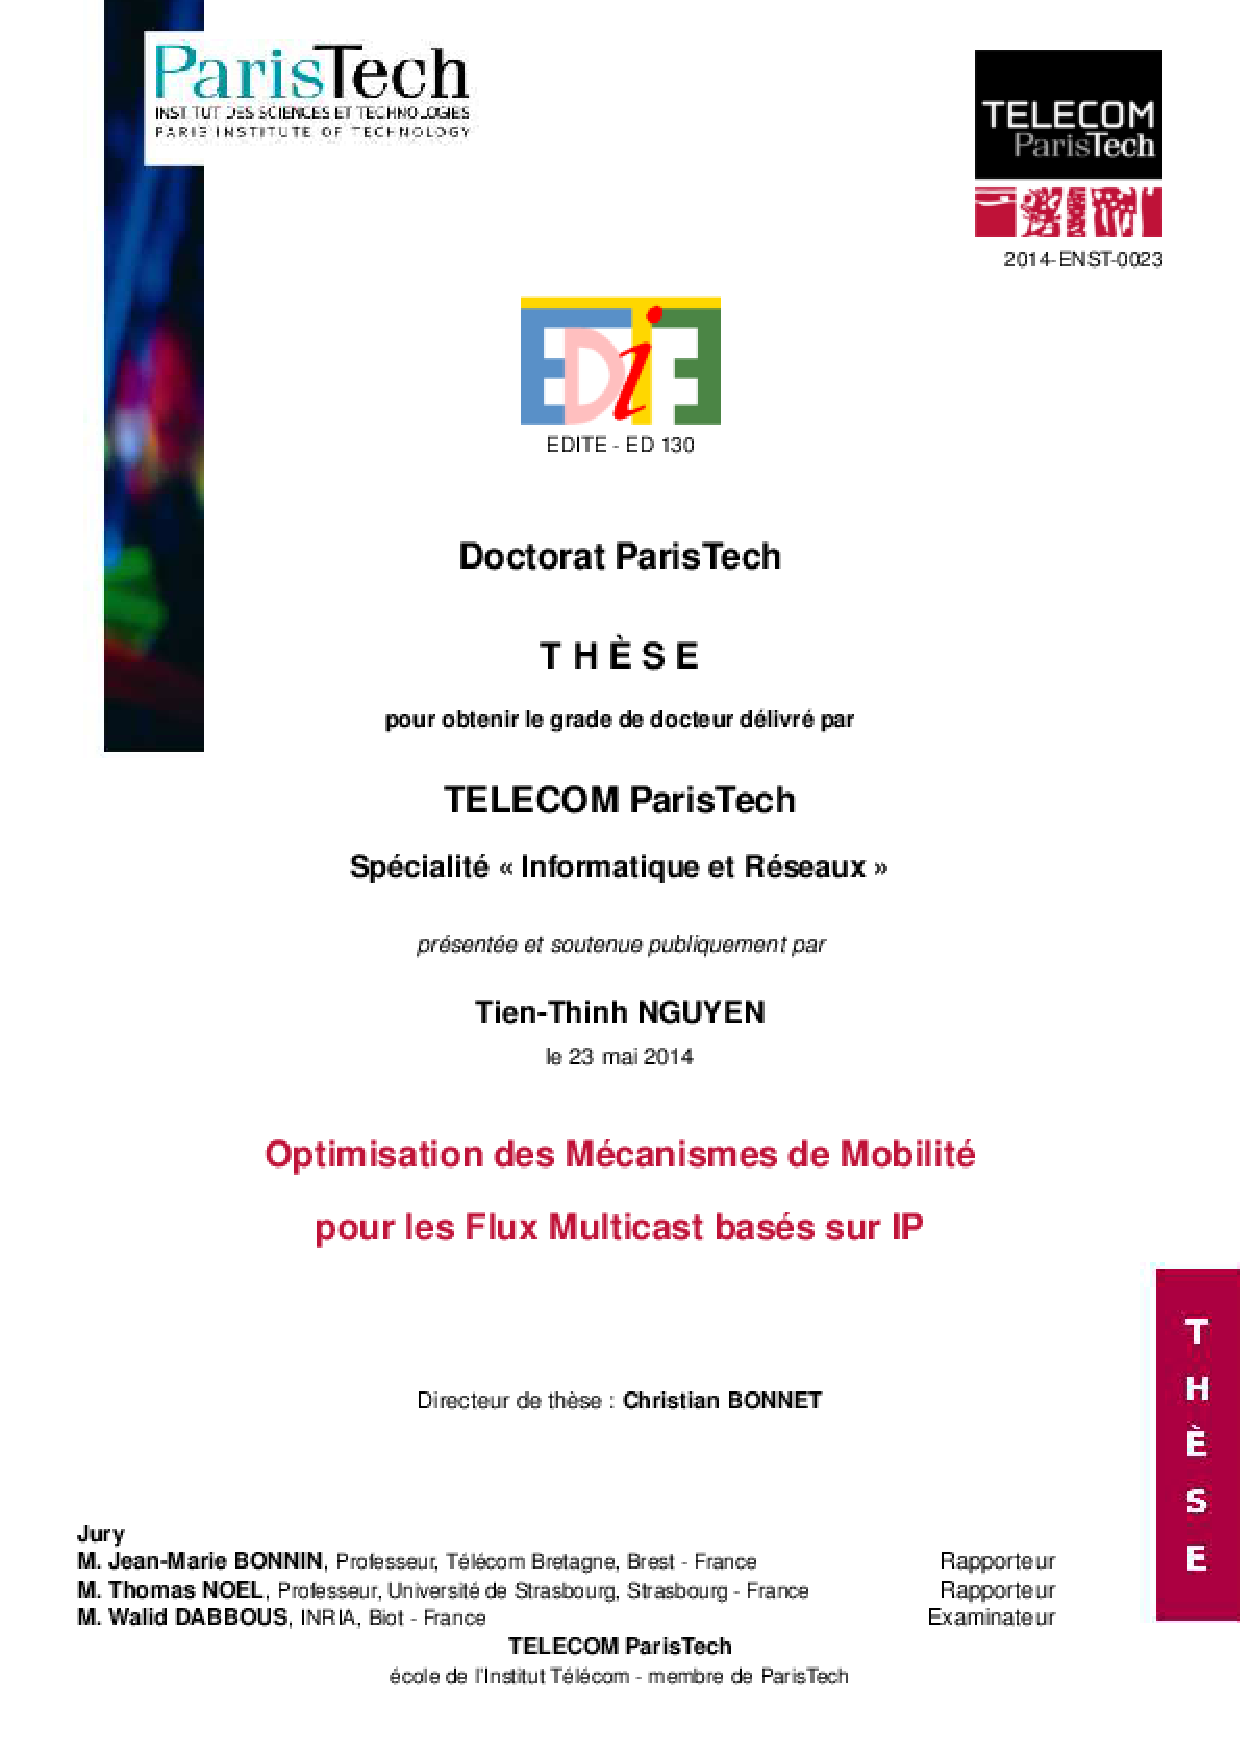
\includepdf[pages={1}]{TPT_Premiere.pdf}

  \vspace{10mm}
  \noindent




	\begin{center}
	
\includegraphics[width=48mm]{logo_ParisTech}
	\end{center}

  \vspace{5mm}


\center

\begin{bfseries}
  \noindent{\LARGE Optimization of Mobility Mechanisms 
\vspace{4mm}
  \\ for IP based Multicast Flows}
  \vspace{15mm}

  \noindent{\Large Tien-Thinh NGUYEN}
  \vspace{10mm}
\end{bfseries}


\noindent{A doctoral dissertation submitted to:}

\vspace{2mm}

\noindent{TELECOM ParisTech}

\vspace{2mm}

\noindent{In Partial Fulfillment of the Requirements for the Degree of:}

\vspace{2mm}

\noindent{\textbf{Doctor of Philosophy}}

\vspace{2mm}

\noindent{Specialty : \textsc{Computer Science and Networking}}

\vspace{2mm}




\vspace{6mm}

\noindent{ \large \textit{Thesis Supervisor:} ~~\textbf{Prof.\ Christian \textsc{Bonnet}}	}

\vspace{2mm}
 
 
\begin{center}
\noindent \large 
\begin{tabular}{llcl}
      \textit{Jury:}	& 		& & \\\\
     \textit{Reviewers:} & & & \\
 \multicolumn{2}{l}{~~\textbf{Prof.\ Thomas \textsc{Noel} }} 		& - & Universit\'{e} de Strasbourg, Strasbourg - France\\
 \multicolumn{2}{l}{~~\textbf{Prof.\ Jean-Marie \textsc{Bonnin}}} 		& - &  T\'{e}l\'{e}com Bretagne, Brest - France\\
\\
      \textit{Examiner:}& 		& & \\
      
\multicolumn{2}{l}{~~\textbf{Dr. \ Walid \textsc{Dabbous}}}           & - & INRIA, Biot - France\\
\\


  
\end{tabular}
\end{center}

\end{titlepage}

}


\cleardoublepage

\pagenumbering{gobble}
\vspace{10mm}

\hfill
  \noindent{
\vspace{4mm}}


\begin{center}
\noindent \large 
\vspace{32mm}
%\noindent{\textbf{To my wife and my little son - Bi}}
 \end{center}

\vspace{3cm}
\dominitoc
\pagenumbering{roman}
\cleardoublepage


%\section*{}
% \vspace{118ex}
% \begin{center}
% \copyright \hspace{1ex}2012\\Tien-Thinh NGUYEN\\ALL RIGHTS RESERVED
% \end{center}
% \cleardoublepage


\addcontentsline{toc}{section}{Acknowledgements}
\markboth{Acknowledgements}{Acknowledgements}
\chapter*{Acknowledgements}

% First of all, I would like to extend my sincere thanks to my advisor Prof. Christian Bonnet for his valuable support and brilliant ideas. Throughout this thesis, he has always found the time for me to guide and encourage my research activities. I also very much appreciate his dynamism and his competences that made this thesis work a success. It has been my real pleasure to work with Christian. \\

% I would also like to thank Prof. Jérôme Härri who helped me so much with his stimulating technical discussions and constructive publication reviewing. A special warm thank to my master advisor Michelle Wetterwald for her kindness and words of wisdom which facilitate not only my research but also my life.\\

% I am grateful to the committee members of my jury, Prof. Jean-Marie Bonnin, Prof. Thomas Noël and M. Walid Dabbous for their valuable inputs and time spent reading this thesis. \\

% I would like to express my appreciation to my colleagues and friends at Eurecom, for all the unforgettable enjoyable moments and their helps. I also wish to extend my warmest thanks to all my friends in France and Vietnam for all the wonderful time we spend together.\\

% Finally, last but not least, I want to express my special gratitude to my parents, my wife and my son for their unconditional support, love and trust. They, together with another members in my big family, make my life full of kindness and happiness with their encouragement.\\

\addcontentsline{toc}{section}{Abstract}
\markboth{Abstract}{Abstract}
\chapter*{Abstract}
% With the development of wireless access technology as well as the explosion of mobile devices (such as smartphones, tablets, and vehicles), the next generation mobile network is not only restricted to provide the traditional voice services but also the data services. Also, the increasing penetration of the mobile devices is generating a huge number of data traffic over mobile networks. In all-IP mobile networks, IP mobility management is a crucial concept to meet the demand of ubiquitous Internet connectivity as well as new service requirements such as seamless handover across heterogeneous networks, consistent quality of experience and stringent delay constraints. In this context, the scalability and bandwidth efficiency from the multicast routing make the IP multicast a valuable solution from the application point of view to deal with a huge number of traffic, particularly, in mobile environments where users usually share frequency bands and limited capacity. But one of the major challenges for the multicast support is when considering mobility. It comes from the fact that the multicast protocols were designed to support the stationary multicast parties. As such, it raises some issues as a result of the interaction of IP multicast and IP mobility protocols such as service interruption, packet loss, routing non-optimal, and packet duplication, etc. In fact, the conventional IP mobility management (e.g., Mobile IPv6 (MIPv6) and Proxy Mobile IPv6 (PMIPv6)) which leverages on the centralized mobility management approach, brings several issues for the network operator like inefficient use of network resources, poor performance, and scalability issues. The concept of Distributed Mobility Management (DMM) aims to tackle these issues and helps the mobile operators address the challenges created by rising mobile usage while enhancing the overall customer experience.\\

% In this thesis, our main objective is to deal with the multicast mobility-related issues. The solutions are proposed in the context of the evolution of the current IP mobility management: from the host-based to the network-based, and also from the centralized to the distributed mobility management. In more details, for a single PMIPv6 domain, we introduce a method to reduce the service disruption and leave latency. We then present a solution from the load balancing point of view to address the service disruption and packet duplication issue. As DMM has not been standardized, we propose an inter-domain mobility solution, which can be considered as a step in the evolution from PMIP towards DMM. Finally, we converge to a final architecture in a DMM environment that can offer various benefits and address most of the multicast listener mobility-related issues. Throughout this thesis, a near-to-real testbed is used to achieve the realistic results.

aa \index{aa}

\clearpage


\addcontentsline{toc}{section}{Contents}
\markboth{Contents}{Contents}

\tableofcontents
\clearpage

\addcontentsline{toc}{section}{List of Figures}
\listoffigures
\clearpage
\addcontentsline{toc}{section}{List of Tables}
\listoftables
\clearpage

%\printnomenclature
\addcontentsline{toc}{section}{Glossary}
\markboth{Glossary}{Glossary}
\chapter*{Glossary}
List of Abbreviations and Acronyms\\
\\
\begin{center}
\begin{longtable}{p{5cm}p{8.8cm}}
% % \hline
\textbf{3GPP} & 3rd Generation Partnership Project\\
\textbf{4G} & Fourth Generation\\
\textbf{AAA} & Authentication, Authorization and Accounting\\
\textbf{ALM} & Application-Layer Multicast\\
\textbf{ASM} & Any-Source Multicast\\
\textbf{aHMAR} & Anchor HMAR \\
\textbf{aNMAR} & Anchor NMAR\\
\textbf{AP} & Access Point\\
\textbf{AR} & Access Router\\
\textbf{A-LMA} & Anchor LMA\\
\textbf{A-AAA} & Anchor AAA\\
\textbf{A-MAG} & Anchor MAG\\
\textbf{BA} & Binding Acknowledgment\\
\textbf{BCE} & Binding Cache Entry\\
\textbf{BU} & Binding Update\\
\textbf{CBT} & Core Based Tree \\
\textbf{CDN} & Content Delivery Network\\
\textbf{cHMAR} & Current HMAR \\
\textbf{C-LBC} & Central Load Balancing Controller\\
\textbf{cMAR} & Current MAR\\
\textbf{CMD} & Centralized Mobility Database\\
\textbf{CMF} & Context Management Function\\
\textbf{cNMAR} & Current NMAR\\
\textbf{CN} & Corresponding Node\\
\textbf{CoA} & Care-of-Address\\
\textbf{COMMA} & Common MMA\\
\textbf{DHCP} & Dynamic Host Configuration Protocol\\
\textbf{DMM} & Distributed Mobility Management\\
\textbf{DMMA} & Dynamic Multicast Mobility Anchor\\
\textbf{DSMIPv6} & Dual Stack Mobile IPv6\\
\textbf{DR} & Designated Router\\
\textbf{DVMRP} & Distance Vector Multicast Routing Protocol \\
\textbf{D-GW} & Distributed Gateway\\
\textbf{eNB} & Evolved NodeB\\
\textbf{EPC} & Evolved Packet Core\\
\textbf{ETF} & Explicit Tracking Function\\
\textbf{EV} & Electric Vehicle\\
\textbf{EVCS} & Electric Vehicle Charging Service\\
\textbf{FA} & Foreign Agent\\
\textbf{FI} & Fairness Index\\
\textbf{FMIPv6} & Fast Mobile IPv6\\
\textbf{FPMIPv6} & Fast Handovers for PMIPv6\\
\textbf{GGSN} & Gateway GPRS Support Node\\
\textbf{GPRS} & General packet radio service\\
\textbf{G2V} & Grid-to-Vehicle\\
\textbf{HA} & Home Agent\\
\textbf{HMAR} & Host-based Mobile Access Router \\
\textbf{HMIPv6} & Hierarchical Mobile IPv6\\
\textbf{HeNB} & Home eNodeB\\
\textbf{HIP} & Host Identity Protocol \\
\textbf{HNP} & Home Network Prefix\\
\textbf{HoA} & Home Address\\
\textbf{HSPA} & High Speed Packet Access\\

\textbf{IANA} & Internet Assigned Number Authority \\
\textbf{ICMD} & Inter-Domain Centralized Mobility Database\\
\textbf{IETF} & Internet Engineering Task Force\\
\textbf{IGMP} & Internet Group Management Protocol\\
\textbf{IFOM} & IP Flow Mobility\\
\textbf{IMR} & Intersection Multicast Router\\
\textbf{IP} & Internet Protocol\\
\textbf{IPTV} & Internet Protocol Television\\

\textbf{L2} & Layer 2\\
\textbf{L3} & Layer 3\\
\textbf{LB} & Load Balancing\\
\textbf{LBC} & Load Balancing Controller\\
\textbf{LIPA} & Local IP Access \\
\textbf{LLQC} & Last Listener Query Count \\
\textbf{LLQT} & Last Listener Query Timer \\
\textbf{LMA} & Local Mobility Anchor\\
\textbf{LMD} & Localized Mobility Domain\\
\textbf{LTE} & Long Term Evolution\\
\textbf{L-GW} & Local Gateway\\
\textbf{MAC} & Media Access Control\\
\textbf{MAG} & Mobile Access Gateway\\
\textbf{MALI} & Multicast Address Listening Interval\\
\textbf{MANET} & Mobile Ad hoc Network \\
\textbf{MAP} & Mobility Anchor Point \\
\textbf{MAR} & Mobile Access Router \\
\textbf{MBMS} & Multicast/Broadcast Multimedia Service\\
\textbf{MBone} & Multicast Backbone\\
\textbf{MBSFN} & Multicast/Broadcast over a Single Frequency Network\\
\textbf{MCTF} & Multicast Context Transfer Function\\
\textbf{MC-Req} & Mobility Context Request \\
\textbf{MC-Res} & Mobility Context Response \\
\textbf{MFC} & Multicast Forwarding Cache \\
\textbf{MGMF} & Multicast Group Management Function \\
\textbf{MIH} & Media Independent Handover \\
\textbf{MIPv6} & Mobile IPv6\\
\textbf{MLD} & Multicast Listener Discovery\\
\textbf{MMA} & Multicast Mobility Anchor\\
\textbf{MMAP} & Multicast by Multicast Agent Protocol\\
\textbf{MMF} & Mobility Management Function \\
\textbf{MN} & Mobile Node\\
\textbf{MN-ID} & Mobile Node's Identifier\\
\textbf{MNP} & Mobile Network Prefix \\
\textbf{MoM} & Mobile Multicast Protocol \\
\textbf{MOR} & Mobile Router \\
\textbf{MOSPF} & Multicast Open Shortest Path First \\
\textbf{MPDSR} & Multicast Protocol With Dynamic Service Range  \\
\textbf{MR} & Multicast Router \\
\textbf{MRIB} & Multicast Routing Information Base \\
\textbf{MSDP} & Multicast Source Discovery Protocol \\
\textbf{MTMA} & Multicast Tree Mobility Anchor \\
\textbf{MUMO} & Multicast Mobility Management Module \\
\textbf{NAI} & Network Access Identifier\\
\textbf{ND} & Neighbor Discovery\\
\textbf{NetLMM} & Network-based Localized Mobility Management  \\
\textbf{NEMO} & Network Mobility\\
\textbf{NI} & Node Information\\
\textbf{NMAR} & Network-based DMM Access Router \\
\textbf{NS-3} & Network Simulator NS-3 \\

\textbf{PBA} & Proxy Binding Acknowledgment \\
\textbf{PBS} & Personal Broadcast Service \\
\textbf{PBU} & Proxy Binding Update\\
\textbf{P-GW} & Packet Data Network (PDN) Gateway\\
\textbf{PIM} & Protocol Independent Multicast\\
\textbf{PIM-DM} & Protocol Independent Multicast - Dense Mode\\
\textbf{PIM-SM} & Protocol Independent Multicast - Spare Mode\\
\textbf{PIM-SSM} & Protocol Independent Multicast - Source Specific Multicast\\
\textbf{pHMAR} & Previous HMAR \\
\textbf{PLC} & Power Line Communication \\
\textbf{pMAR} & Previous MAR\\
\textbf{PMIPv6} & Proxy Mobile IPv6\\
\textbf{pNMAR} & Previous NMAR\\
\textbf{Proxy-CoA} & Proxy Care-of-Address\\

\textbf{QI} & Query Interval\\
\textbf{QRI} & Query Response Interval\\

\textbf{RIB} & Routing Information Base\\
\textbf{RPF} & Reverse Path Forwarding\\
\textbf{RV} & Robustness Variable\\

\textbf{SDN} & Software Defined Networking\\
\textbf{SGSN} & Serving GPRS Support Node\\
\textbf{SIP} & Session Initiation Protocol\\
\textbf{SIPTO} & Selected IP Traffic Offload\\
\textbf{SMR} & Session-to-mobility Ratio \\
\textbf{SPT} & Shortest Path Tree \\
\textbf{SSM} & Source-Specific Multicast\\
\textbf{S-GW} & Serving Gateway\\
\textbf{S-AAA} & Serving AAA\\
\textbf{S-LMA} & Serving LMA\\
\textbf{S-MAG} & Serving MAG\\

\textbf{tLMA} & Target LMA\\
\textbf{TLV} & Type-length- vector\\
\textbf{tMAR} & Typical location MAR\\

\textbf{RA} & Router Advertisement \\
\textbf{RADIUS} & Remote Authentication Dial In User Service\\
\textbf{RAN} & Radio Access Network \\
\textbf{RBMoM} & Range-Based Mobile Multicast  \\
\textbf{RP} & Rendezvous-Point\\
\textbf{RPT} & Rendezvous-Point Tree\\
\textbf{RO} & Route Optimization\\
\textbf{RS} & Router Solicitation\\
\textbf{RTT} & Round-Trip Time\\

\textbf{UDP} & User Datagram Protocol \\
\textbf{UE} & User Equipment \\
\textbf{UGC} & User Generated Content \\
\textbf{UML} & User-Mode Linux\\
\textbf{UNP} & Update Notification Message\\
\textbf{V2G} & Vehicle-to-Grid\\
\textbf{VoIP} & Voice over IP\\
\textbf{WiMAX} & Worldwide Interoperability for Microwave Access\\

\end{longtable}
\end{center}

\clearpage

\mainmatter
\chapter{Introduction}
\label{intro}
\section{Motivation and Problem Statement}
With the development of wireless access technology as well as the explosion of mobile devices (such as smartphones and tablets), the next generation mobile network is not only restricted to provide the traditional voice services but also the data services. In other words, it is evolving towards all-IP systems. In fact, the mobile data services have become an essential part of many consumers' lives \cite{cisco_forecast,data_services}. So far, users are using their mobile devices not only for personal life but also for work on a regular basis \cite{cisco_service,morgan_stanley, mobile_2010}. As a result, the mobile data traffic has been almost doubled each year during the last few years\footnote{The increasing traffic is mainly driven by mobile video traffic} \cite{cisco_forecast, ericsson}. This trend is expected to continue in the upcoming years, especially with the deployment of fourth generation (4G) networks. Despite the increasing volume of traffic, the average revenue per user is falling fast \cite{mobile_europe}. In addition, in all-IP mobile networks as mobile nodes may frequently change their point of attachment to the IP network, IP mobility management is a crucial concept to meet the demand of ubiquitous Internet connectivity as well as new service requirements such as seamless handover across heterogeneous networks, consistent quality of experience and stringent delay constraints. Mobility can be handled at different layers of protocol stack ranging from the link layer to the application layer, however, most of these mobility management protocols are located at the network layer. Mobile IPv6 (MIPv6), the first mobility protocol standardized by the Internet Engineering Task Force (IETF) for IPv6 networks, maintains the mobile node (MN)'s reachability when it is away from home. It is done by relying on a central mobility, namely Home Agent (HA). However, in MIPv6, the MN needs to perform the mobility-related signaling, that means the MIPv6 protocol stack is required at the MN. It is the main obstacle of the deployment of MIPv6 in the real world. For this reason, Proxy Mobile IPv6 (PMIPv6), as a network-based mobility management, helps to avoid the additional deployment in the MN so that the MN can be kept simple. In other words, mobility can be transparently provided to all legacy MNs. \\

The mobile network operators are being challenged by the increase of mobile data traffic (especially the video traffic) and the new requirements e.g., providing connectivity anywhere and at anytime with consistency of user experience, while preserving the economics of their networks and creating new opportunities for revenue growth. Faced with these challenges, the operators are seeking for innovative solutions to improve their network performance and efficiency, as well as to reduce the costs expended on network operation and maintenance. Two major focuses are: i) increasing the capacity of wireless communication systems;  and ii) designing and implementing an efficient system to deliver the data. Regarding the first aspect, further dramatic increases in radio capacity of mobile broadband will come with the implementation of new wireless technologies such as Worldwide Interoperability for Microwave Access (WiMAX), High Speed Packet Access (HSPA) and Long Term Evolution (LTE). However, spectrum for operators is both limited and expensive. Thus, they are looking at different methods to increase the system capacity such as deploying femto and pico cells, together with selecting the offload traffic between the licensed and unlicensed spectrum (e.g., from 3G to WiFi). Considering the second aspect, the aim is to simplify the network architecture as well as optimize the data transmission costs. Accordingly, the mobile network is currently evolving towards flat architecture. One example is Local IP Access/Selected IP Traffic Offload (LIPA/SIPTO) architecture defined by the 3rd Generation Partnership Project (3GPP). Following the same idea, IETF has recently chartered the Distributed Mobility Management (DMM) working group which specifies the solutions to address the problems and limitations of the current centralized mobility management. In fact, the conventional IP mobility management (e.g., MIPv6 and PMIPv6) leverages on the centralized mobility management approach, thus,  raises several issues for the network operators like inefficient use of network resources, poor performance, and scalability issues when considering a large number of mobile devices and their traffic demand \cite{DMM_requirements, DMM_issues,DMM_problem_statement}. DMM is one of the solutions to help the mobile operators address these limitations while enhancing the overall customer experience.  \\


As Internet is widely deployed and spread across a large area, it carries a variety of common information resources and services. In a sharing world, the group communication service, which refers to the ability to send data to several receivers at the same time, is naturally becoming more and more important especially in some areas like multimedia distribution, gaming, and financial services, etc. In this context, the scalability and bandwidth efficiency from the multicast routing make the IP multicast a remarkable solution from the application point of view to allow the mobile networks to deal with a huge number of traffic, particularly, in mobile environments where users usually share frequency bands and limited capacity \cite{Multicast_MIPv6}. But one of the major challenges for multicast support is when mobility is considered. It comes from the fact that the multicast protocols were designed to support the stationary multicast parties. As such, it raises some issues as a result of the interaction of IP multicast and IP mobility protocols e.g., transparency, routing optimization, packet duplication, service disruption, packet loss and group leave latency, etc \cite{Multicast_MIPv6, multicast_challenges_solutions}.\\
 
Regarding the IP mobile multicast, after more than a decade of research and development efforts, many approaches have been proposed, but most of them are based on such host-based mobility management protocols as MIPv6, Fast Mobile IPv6 (FMIPv6) and Hierarchical Mobile IPv6 (HMIPv6). However, the main drawback of these protocols is that they require the MN to modify its IP stack to participate into the mobility signaling process. In fact, it is the major obstacle of the deployment of MIPv6 in the real world. Additionally, the previous IP multicast approaches cannot be directly applied in a network-based mobility management in which the MN is unaware of mobility process. To solve the aforementioned issues, the IETF has worked in different solutions highlighting the difference between the source and the listener multicast mobility problems in PMIPv6. However the proposed solutions remain unable to address the issues of scalability, performance optimization and compatibility with unicast mobility at the same time. In DMM, there is no complete solution for the multicast mobility support.\\

It is generally acknowledged that a proposed solution cannot be widely accepted without results from valid experimentation. Such validation nowadays can be obtained through various methods, each with its own advantages and limitations. Within the networking field of research, the results’ reliability is one of the most critical issues. Thus, the results credibility is directly related to the methods used, therefore improving them becomes of great importance. In this context, the most widely used method - simulation - sometimes lacks credibility. The lesser used but most credible method - real testbed - is too expensive and difficult to scale and manage. \\

In this thesis, our objective is to deal with the multicast-related issues raised when a multicast node moves in a network-based mobility management domain. In other words, the aim of this research is to find solutions that ensure:
\begin{itemize}
\item Keeping the MN unaware of mobility from the multicast service point of view;
\item Minimizing the service disruption time to even satisfy the strict requirements for the interruption- and delay-sensitive services;
\item Keeping the signaling/tunneling overhead as low as possible;
\item Maximizing the available network resource (reducing the waste of resources and packet duplication), keeping the reliability and improving the scalability of the system;
\item Minimizing the modifications of the mobility management and the multicast routing protocols to support IP mobile multicast. 
\end{itemize}
\begin{figure}[h!] 
 \begin{center} 
 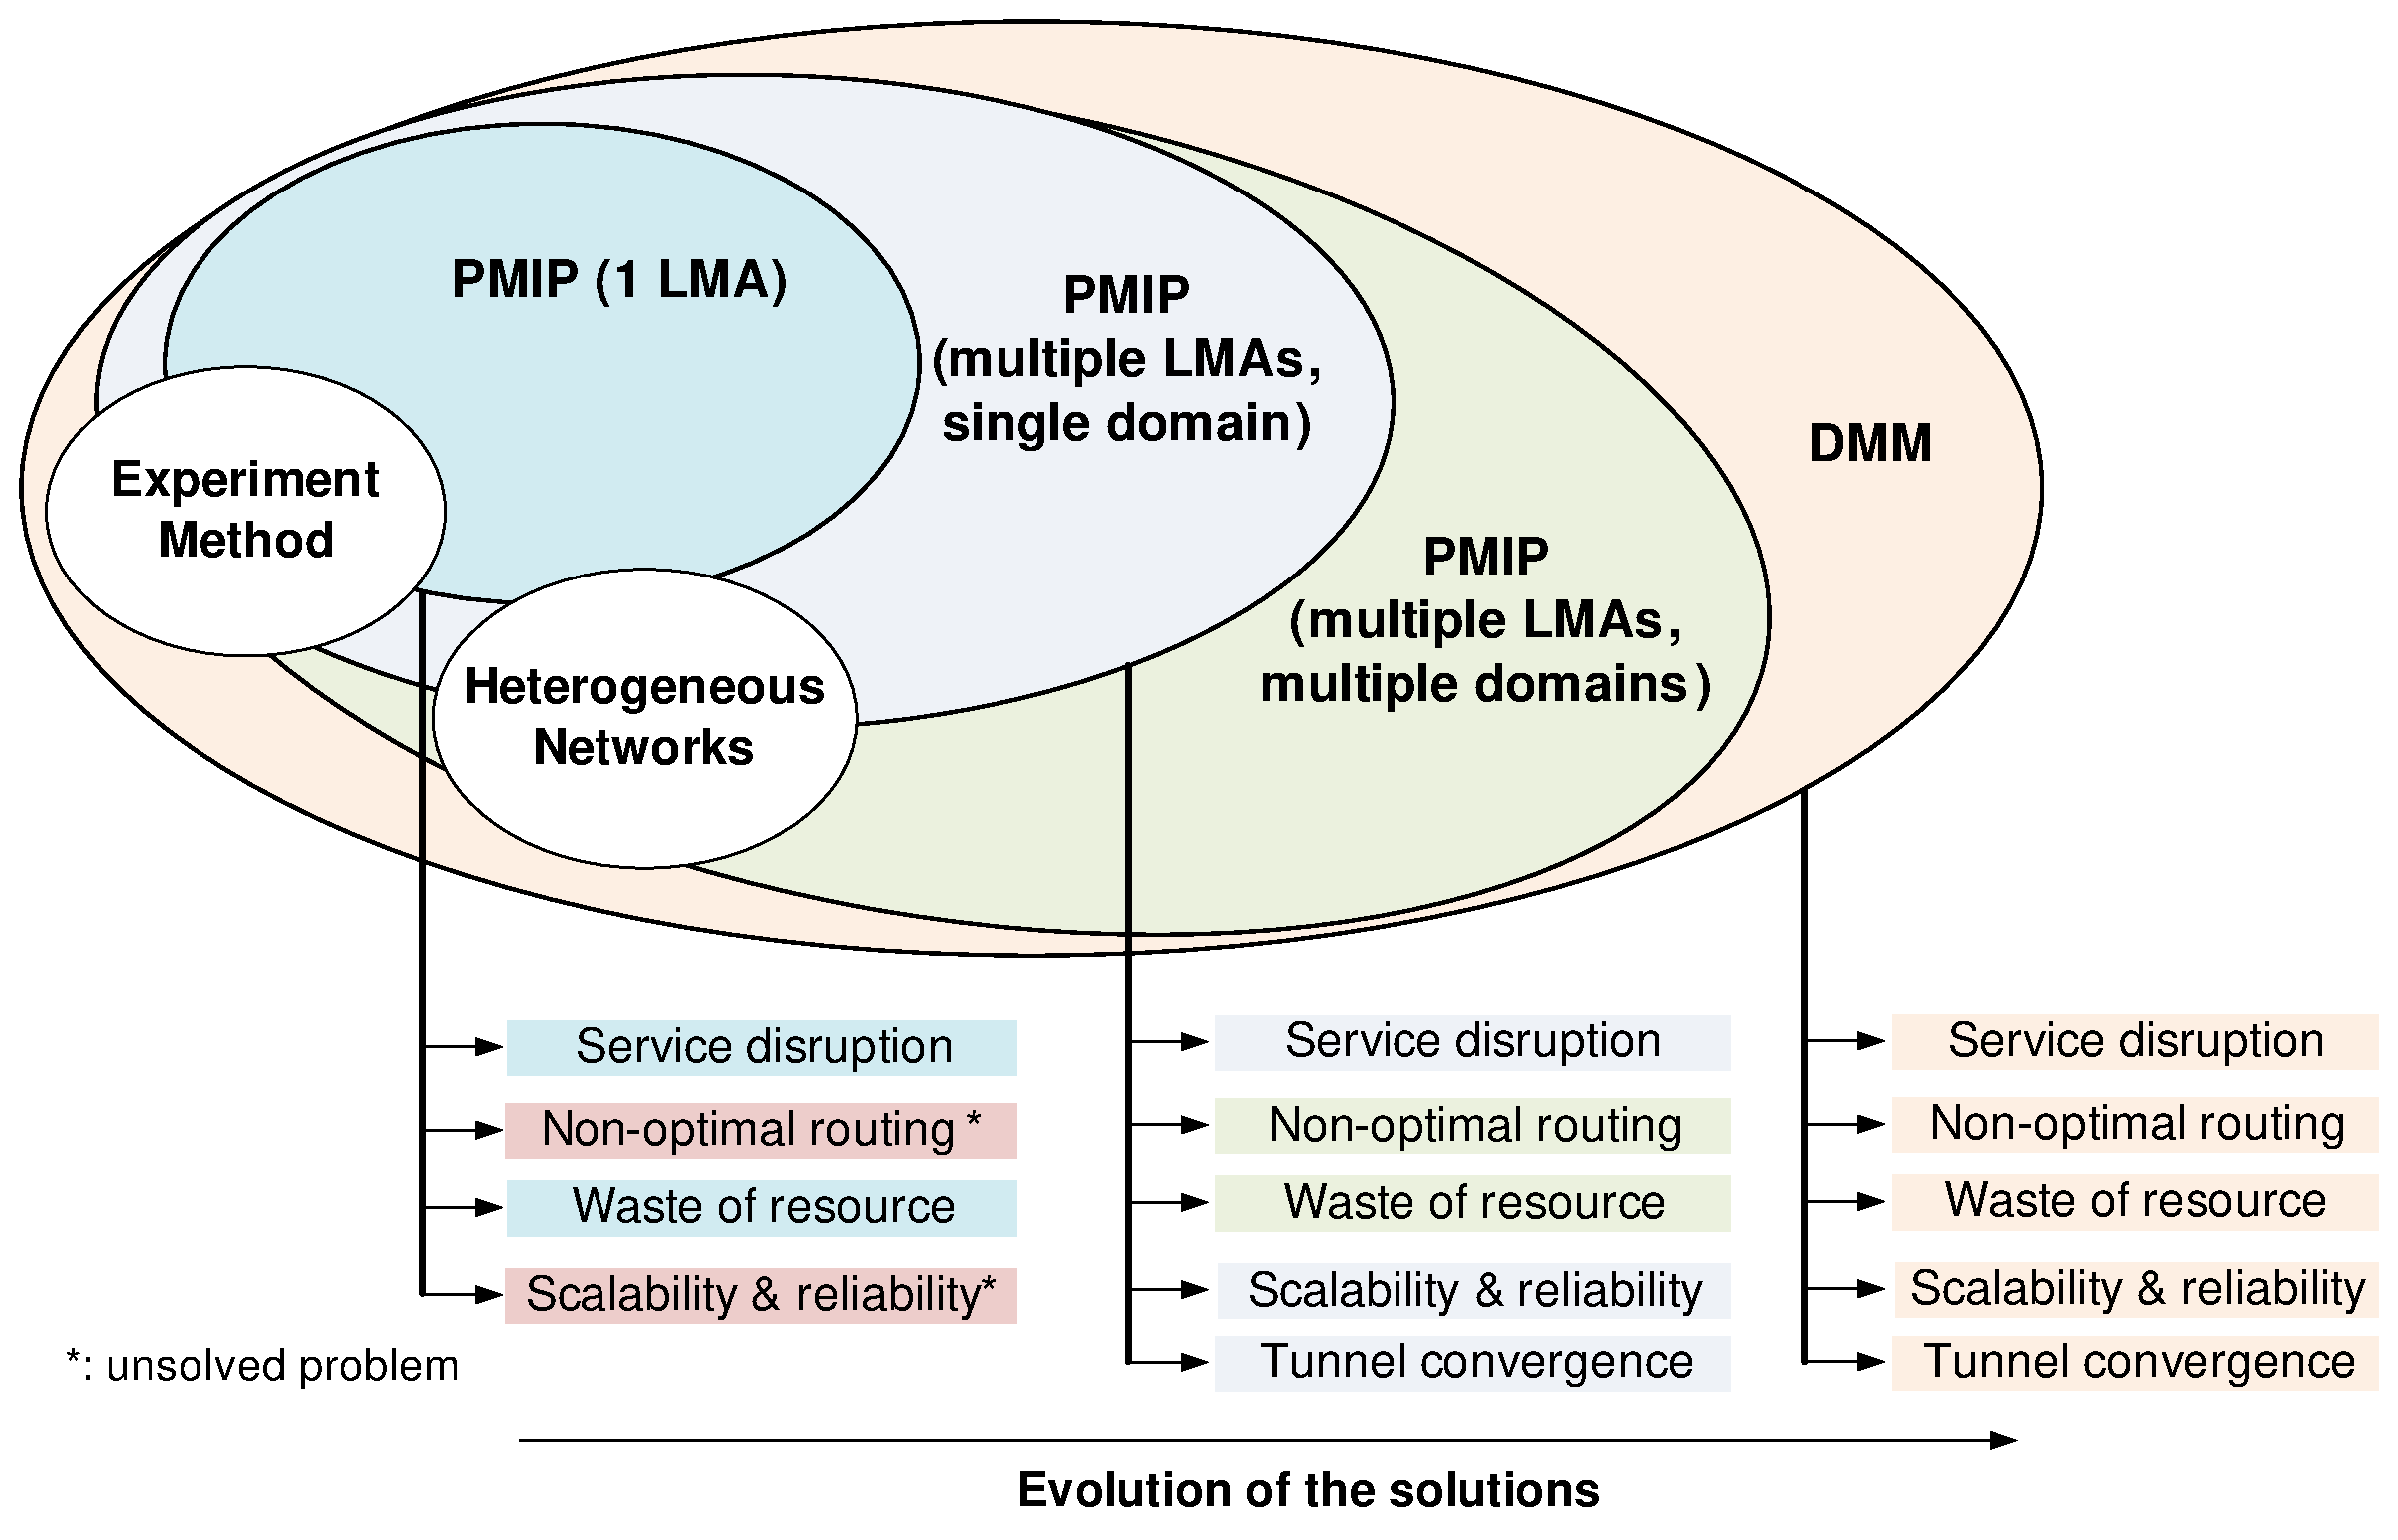
\includegraphics[width=0.72\textwidth]{./Introduction/Chapter1/figures/vision.eps} 
    \caption{Evolution of the solutions for multicast mobility.}
     \label{fig:vision}
  \end{center} 
\end{figure}
The evolution of the solutions for multicast mobility is illustrated in Fig.~\ref{fig:vision}. For a single PMIPv6 domain (with one local mobility anchor (LMA)), we introduce a method to minimize the service disruption time considering both cases: a mobile node with single or multiple interfaces. The waste of resources caused by a long leave latency is also reduced. On the other hand, the non-optimal routing; scalability and reliability issues are unsolved. Considering a single PMIPv6 domain with multiple LMAs, an additional issue is introduced - the tunnel convergence problem (or packet duplication). To improve the scalability and reliability for PMIPv6 network while addressing the tunnel convergence problem, the load balancing mechanism is proposed at an acceptable cost of service disruption. As DMM is still under discussion and has not been standardized, we provide an inter-domain mobility support which can be considered as a step towards the deployment of DMM. IP multicast then will be considered in both the inter-domain and the DMM environments. Taking benefits of the previous proposed solutions, the dynamic multicast mobility anchor (DMMA) mechanism in DMM addresses almost all the multicast mobility-related issues such as service disruption, non-optimal routing, waste of resources, tunnel convergence and scalability. Additionally, throughout our thesis, a near-to-real testbed will be used to achieve the realistic results. 

\section{Thesis Contributions and Outline}
The key contributions to the study of IP mobile multicast proposed in this thesis can be summarized as follows.
\paragraph{PMIP-based solutions}
\begin{itemize}
\item \textit{A method to minimize the multicast service disruption time during handovers inside a PMIPv6 domain}: This solution is based on the multicast context transfer and the explicit tracking function. Then, a PMIPv6 testbed has been deployed, which allows simulating the mobility of multiple multicast sources and listeners at the same time. A real implementation of the multicast context transfer function and the explicit tracking function has been deployed. Also, the listener part of Multicast Listener Discovery Version 2 (MLDv2) has been developed in NS-3.

\item \textit{A multicast-based load balancing mechanism among LMAs to solve the problem of bottleneck and single point of failure at the LMA}: This mechanism taking multicast into account helps to better distribute the load caused by the multicast flows in a PMIPv6 domain. Also, this solution can co-operate with the existing load balancing mechanisms to enhance the scalability and reliability of the system. 

\item \textit{Mobility in heterogeneous networks discussions via a use case: electric vehicle charging service (ECVS)}: By using PMIPv6, the service takes care of the Electric Vehicle (EV) mobility, handling vertical and horizontal handovers between different communication technologies (e.g., Wireless LAN (WLAN), LTE and Power Line Communication (PLC)). The IPv6 address preservation in PMIPv6 is guaranteed by relying on the logical interface mechanism which helps to hide the change of interface to the IPv6 stack. Moreover, the logical interface keeps the MN unaware of the interface change as well as mitigates its impact on the service disruption. 
\end{itemize}

\paragraph{DMM-based solutions}
\begin{itemize}
\item \textit{A solution for inter-domain mobility for PMIPv6}: It allows the data packets to be routed via a near-optimal way by bringing the mobility anchors closer to the MN while the control management can be placed anywhere in the network. This solution can be considered as a one step towards the deployment of DMM. A basic support for the multicast listener mobility in an inter-domain environment then is provided.  

\item \textit{A dynamic multicast mobility anchor selection in DMM (DMMA)}: It enables a per-flow multicast support. From a multicast service perspective, it helps satisfy the requirements in terms of service disruption and delay, especially when considering the real-time services. The packet duplication and waste of resources (or leave latency) issues can be reduced. Also, it provides a mechanism to better distribute the load among the Mobile Access Routers (MAR). The DMMA mechanism takes the advantages from the previous contributions into account, for example: i) the multicast context transfer and explicit tracking function are re-used to minimize the service disruption; ii) the load information is used as a metric for the multicast anchor selection; iii) the method of load collection is applied to collect others metrics; and iv) the operation of the central mobility database (CMD) is similar to the inter-domain central mobility database from the inter-domain PMIPv6 proposal. 
\end{itemize}

In order to validate the solutions with a high degree of confidence, \textit{an experiment method is used to achieve the realistic results at low cost}. This is a trade off between the simulation method which in some cases lacks of credibility and the real testbed which is typically too expensive, difficult to scale and manage. Based on this method, a testbed is deployed to conduct the experiments for the multicast mobility in PMIPv6. Additionally, this method can be generally applied for the experimentation in wireless mobile networks.  \\

The work presented in this thesis is structured as follows. A part from the introduction and final conclusion, we divide the content of the thesis into three main parts. We present a brief description of the related works in the first part. Then, in part II and III, we discuss the solutions for the mobile multicast-related issues.

\begin{enumerate}
\item In the first part, we provide an overview of IP multicast and IP mobility. This part also highlights the issues and challenges when considering multicast in a mobile environment. Particularly, we make a brief introduction of the main approaches proposed by the IETF regarding their advantages and limitations. Based on this analysis, the solutions for the remained issues will be presented in the next parts. Also, we enlist the requirements for an effective performance evaluation of mobile multicast solution. We then propose an efficient method for experimentation in the wireless mobile networks. The testbed, which is developed based on this method, will be used throughout this thesis to validate the solutions. 

Results have been presented and / or published
\begin{enumerate}
\item in the Future Network and Mobile Summit (Futurenet 2012) \cite{Thinh_futurenet}
\item within an official research deliverable of Medieval \cite{d4.2, d4.3}
\end{enumerate}

\item The second part discusses several issues when a multicast node moves in a single PMIPv6 domain. Chapter \ref{ch:multicast_PMIP} focuses on the service disruption issue. Chapter \ref{ch:LB} proposes a load balancing mechanism taking multicast service into account to better distribute the load among LMAs, so as to improve the scalability and the reliability of the PMIPv6 domain. Chapter \ref{ch:EVCS} discusses the mobility of a multihomed node in which the logical interface mechanism is used to hide the change of physical interface to the IP stack.

Results have been presented and / or published
\begin{enumerate}
\item at the Wireless Communication and Networking Conference (WCNC 2013) \cite{Thinh_WCNC_Multicast}
\item at the 24th Annual IEEE International Symposium on Personal, Indoor and Mobile Radio Communications (PIMRC 2013) \cite{PMIP_EV}
\item at the CNC workshop, 2014 International Conference on Computing, Networking and Communications (ICNC 2014) \cite{Thinh_ICNC}
\end{enumerate}

\item In the last part, we first propose an inter-domain mobility support for PMIPv6 based on the DMM concept in Chapter \ref{ch:inter_domain}. Then in Chapter \ref{ch:multicast_dmm}, we propose a dynamic multicast mobility anchor selection in DMM which enables a per-multicast flow support. The proposed mechanism helps satisfy the requirements in terms of service disruption and delay, especially when considering real-time services. Also, it provides a mechanism to better distribute the load among the MARs. 

Results have been presented and / or published
\begin{enumerate}
\item at the International Conference on Communications (ICC 2014) \cite{Thinh_ICC}
\item at the 78th Vehicular Technology Conference (VTC2103-Fall) \cite{Thinh_VTC}
\item at the Wireless Communication and Networking Conference (WCNC 2013) \cite{Thinh_WCNC_DMM}
\item at the 9th International Conference on Networking and Services \cite{Thinh_ICNS}
\item at the International Conference on Communications (ICC 2013) \cite{ICC_Sergio}
\end{enumerate}
\end{enumerate}

The contributions of this thesis have also been submitted to the Computer Networks journal, Elsevier \cite{Thinh_elsevier_LB} and will be submitted to the Wireless Networks journal, Springer \cite{Thinh_Springer}.





\part{Background Analysis\label{pa:part1}}

\chapter*{Overview of Part \ref{pa:part1}}

In this part, we will introduce the fundamental notions, elements of Internet of Things as well as identity the common issues and challenges when deploying IoT solutions in large scale. We then analyze in detail Interoperability and Reliability issues in CloudIoT paradigm. The  most relevant work related such problems are also discussed.



\chapter{Reference Technologies and Challenges}
\label{ch:reference_technologies}
\section{Overview Internet of Things and Related Concepts }
\subsection{Internet of Things}
The concept of Internet of Things was first coined by Kevin Ashton, Executive Director of the Auto-ID Center in Massachute Institute of Technology (MIT) in 1999, and it is described as a world where billions of objects can sense, communicate and share information \cite{madakam2015internet}. Then IoT becomes more popular due to the explosion of mobile devices, ubiquitous communication, cloud computing. However, the definition of ``Internet of Things'' is still ambiguous, and have different facets depending on the perspective. From the view of functionality and identity, IoT is defined as ``Things having identities and virtual personalities operating in smart space using intelligent interfaces to connect and communicate within the social, environmental, and user contexts'' \cite{ray2018survey}. Semantically, the term of Internet of Things is composed of two words ``Internet'' and ``Things''. Following this way, IoT could be defined as ``a worldwide network of interconnected object uniquely addressable, based on standard communication protocols''~\cite{minerva2015towards}.\\

Similar to its definition, the characteristic of IoT vary from one domain to another. Some of the key characteristics identified during the research study are as follows:
\begin{itemize}
    \item \textbf{Dynamic and Self-adapting}: IoT devices and system must be able to dynamically adapt with the changing contexts or sensed environment. For example: considering a smart building system comprising of a number of temperature devices. These devices can adapt their modes based on whether it is indoor or outdoor. Based on that, they can adjust the calibrations to collect data more accurately. In this example, the smart building system is adapting itself with the change of context or environment.
    
    \item \textbf{Self-configuring}: IoT device may have the capability to configure themselves relating connection, software upgrades, etc., while minimal user intervention.  This characteristic allows co-operating a large number of devices to provide specific functionality.
    
    \item \textbf{Interoperable Communication Protocols}: The IoT devices may support multiple connectivity (Wifi, Lora, Sigfox, etc.) to communicate with other devices as well as the cloud infrastructure.
    
    \item \textbf{Unique Identify}: IoT device must be identified by a unique identity (such as an IP address or an URL). In addition, the IoT system needs to provide intelligent interface allowing the end-user to access directly these devices.
    
    \item \textbf{Integrated into Information Network}: In order to communicate and exchange data, IoT devices are integrated into the information network. In addition, these devices can be dynamically described and discovered in the network by other IoT devices or systems. For example A weather station can describe its monitoring information to other station in the same information network so that they can communicate and exchange collected data. Such integration could enrich the acquired information because of the data aggregation from several nodes.
    
\end{itemize}

\subsection{Web of Things and Semantic Web of Things}
Recent years, we have been witnessing the explosion of Internet of Things in term of the number and types of IoT devices. Unfortunately, there is no universal application protocol that is compatible with various networking interface. Thus, building a single global ecosystem of Things communicating with each other seamlessly is still impossible~\cite{WebofThi19:online}. In other words, the IoT is a collection of ``Silos of Things'' that can not interact with each other. Therefore, to build a global Internet of Things, we need a universal language and protocols supporting the interaction between devices and application regardless their properties (types, firmware, configuration, etc.). Instead of inventing a dedicated technology, leveraging the widely popular web protocols, standards, and blueprints to make data and services offered by Things more accessible to a larger pool of developer~\cite{guinard2016building}. That is premise behind adoption of the Web of Things. The ultimate goal of Web of things is effectively breaking the ``Silos of Things'' also known as ``one device, one protocol, one app'' by applying tools and techniques that are available on the Web technology.

In order to archive its goals, WoT is used on the Application level to abstract the complexity and variety of lower-level (protocols, firmware, data formats, etc.) by a simple Web model to facilitate the integration of all IoT devices and application. In other words, by hiding the heterogeneity of IoT devices and application behind Web technologies, the WoT allows developers to focus on their application without considering the technologies behind. In practice, the developers could interact with IoT Things via web browsers and explore the Things as surfing the web. The collected data from Things is visually displayed using Web programming language such as HTML, CSS, and Javascript. 

In general, the Web of Things facilitates the interaction and exchange of information between different Things and System powered by Web technologies. However, the exchanged data can be encoded and presented under different formats (envelopes, semantics, and meta-data) . For example, the collected data presenting current temperature can be under plain text, XML/EXI, or JSON format. The file name can be ``temperature'' or ``temp''. Therefore, it is necessary to build a Semantic Web of Things (SWoT) to ensure a common understanding and format. In other words, SWoT concept is the evolution of the Web on Things with the Semantic technology. The goal of SWoT is to provide comprehensive interoperability that allows not only sharing and reuse of IoT Things but also making IoT data to be universally understandable~\cite{pfisterer2011spitfire}. The summary of evolution from Internet of Things to Web of Things is illustrated in Figure~\ref{fig:c2_evolution_iot_swot}

\begin{figure}[h!] 
 \begin{center} 
 \includegraphics[width=0.72\textwidth]{./Part1/Chapter2/figures/c3_evolution_iot_swot.jpg} 
    \caption{Evolution of the solutions for multicast mobility.~\cite{jara2014semantic}}
     \label{fig:c2_evolution_iot_swot}
  \end{center} 
\end{figure}

\subsection{Massive Internet of Things}
With the explosion of Internet of Things, the number of Things and its connectivity have been growing exponentially. In addition, Things is no longer just send the data to cloud, but also exchange information to each other. As a result, Massive IoT is emerging as a new focal point for IoT connectivity technologies referring to huge volume of constrained IoT devices, which stringently require excellent coverage, cost-effective and low-energy consumption~\cite{Northstream2017}. Among several new connectivity technologies for MIoT, proprietary LPWAN technologies such as Sigfox and LoRA have been considering the most potential candidates while cellular-based connectives such as 5G or NB-IoT are under developing and testing process \cite{raza2017low}.

On a technical level, the IoT devices in Massive Internet of Things context are distributed in a wide area from large manufacturing plants to inside sewer systems where the radio signal is physically challenging. To adapt to such environments, the connectivity technology of Massive IoT is not only wide coverage but also robust. In addition, replacing device battery in large area is very expensive. This connectivity technology must be low energy consumption to extend the device battery life. Typically, high throughput and latency are not unessential in massive IoT applications, since they more focus on collecting data than controlling.


\section{Fundamentals of IoT}
\subsection{IoT Things}
Similar to Internet of Things definition, deriving a unified definition for the ``Things’’ in IoT is still challenging although it has received most attention from academic organizations such as NIST, ITU, W3C, IERC, and IETF~\cite{Liu2016}. IEEE simply defined the Things as a physical object that is relevant from a user or application perspective~\cite{minerva2015towards}. However, IERC believes that a Thing can be physical or virtual and identified by unique identity~\cite{smith2012internet}. NIST proposes the Things can be all software, all hardware, or the combination of software and hardware.~\cite{voas2016networks}. 

Due to the heterogeneity in Things definition, we simplify the Thing could be physical or virtual object integrated into a network. This object can interact via a unique identity and intelligent interface. For example, a smart phone can be a Thing which is physical object, able to join networks (WiFi, cellular network), has unique identity (phone number, IP address) and intelligent interface. A database is also considered as a Thing because it is a virtual object, able to join networks (internet), has unique identity (URL) and intelligent interface (Web services).
\subsection{IoT Connectivity}
In this section, rather than mentioning all the IoT protocol following existing architecture model like OSI models, we only present some dedicated protocols in IoT and organize them based on their functionality.

\begin{description}
\item[\textbf{Infrastructure}:\\]
    \begin{itemize}
    \item[] 
    \item \textit{6LoWPAN: } This is an acronym of IPv6 over Low Power Wireless Personal Area Networks defined by the Internet Engineering Task Force, IETF in their document RFC 6282~\cite{shelby20116lowpan} deriving from the idea that "the Internet Protocol could and should be applied even to the smallest devices,"~\cite{Mulligan:2007:ARC:1278972.1278992}. This protocol uses 2.4 GHz frequency with 250 kbps rate.
    
    \item \textit{uIP: } The uIP is an open source project licensed under a BDS style license~\cite{adamdunk86:online}. The goal of this project is to create a dedicated TCP/IP stack for 8 or 16 bits micro-controllers. Currently, it is further developed by wide community.
    
    \item \textit{NanoIP: } The concept NanoIP is to optimize all features of Internet to adapt to embedded and small devices, without the overhead of TCP/IP~\cite{shelby2003nanoip}.NanoIP uses two dedicated transport techniques are nanoUPD and nanoTCP. A socket-compatible API is also provided to make sure the protocol similar to original IP protocol.
    
    \item \textit{Time Synchronized Mesh Protocol (TSMP): } TSMP is a communication protocol designed for self-origanizing network of wireless devices enabling reliable, low power, secure communication~\cite{pister2008tsmp} 
    
    \end{itemize}

\item[\textbf{Discovery}:\\]
    \begin{itemize}
    \item[] 
    \item \textit{mDNS: } The mDNS is used to resolves host names to IP addresses within small networks. Except do not include a local name server,  this technology is essentially the same with the unicast Domain Name System (DNS) in term of programming interfaces, packet formats and operation~\cite{cheshire2013multicast}. 
    \item \textit{Physical Web: } The Physical Web aims to discover and interact with nearby devices through a list of URLs being broadcast. That means every smart object in the network needs to broadcast its access URL that any nearby device can receive. 
    \item \textit{HyperCat: } HyperCat is an open, lightweight JSON-based hypermedia catalogue format to exploit Thing resources~\cite{HyperCat76:online}. It allows adding a set of semantic annotations to Things resources and make them discoverable over the web. 
    \item \textit{Universal Plug and Play (UPnP): } The UPnP uses Internet and Web protocols to automatically discover new devices to be plugged into a network. These new devices announce their presence to other devices by using a discovery protocol based on HTTP~\cite{RFC6970U68:online}. 
    
    
    \end{itemize}

\item[\textbf{Data Protocol}:\\]
    \begin{itemize}
    \item[] 
    \item \textit{Message Queuing Telemetry Transport (MQTT): } MQTT \index{MQTT} is an publish-subscribe based messaging protocol working on the top of TCP/IP protocol. It is useful for connections limited bandwidth~\cite{}. An MQTT system consist of a central messaging server named "message broker" and clients. There are two client types are: (1) publisher: clients publish data to broker. (2) Subscriber: Clients receive data from broker. The responsibility of broker is to forward data from publishers to subscribers. 
    
    \item \textit{Constrained Application Protocol (CoAP): } CoAP \index{CoAP} is an application layer protocol designed for constrained internet devices that are limited in storage, computation power. It is based on RESTful protocol design to simply translate to HTTP for simplified integration, while also meeting specialized requirements such as multicast support, very low overhead, and simplicity~\cite{RFC7252T93:online}. Currently, the major standardization for CoAP is done by The Internet Engineering Task Force (IETF) and various new functionalities have been added~\cite{colitti2011integrating}. 
    
    \item \textit{Extensible Messaging and Presence Protocol (XMPP): } XMPP \index{XMPP} is a real-time communication protocol based n Extensible Markup Language (XML). It is defined in an open standard managed by The Internet Engineering Task Force (IETF). Dsigned to be extensible, the protocol is also used for publish-subscribe model in VoIP~\index{VoIP}, video and IoT application \index{IoT!application}. 
    
    \item \textit{Advanced Message Queuing Protocol (AMQP): } Similar to XMPP\index{XMPP}, AMQP is an open standard application layer but it is designed for message-oriented middleware. Thereby, its functionalities ensure reliability and security such as message orientation, queuing, routing~\cite{o2007toward}. The authentication and encryotion based on Simple Authentication and Security Layer(SASL)\index{SASL} or Transport Layer Security (TLS)\index{SASL}
    
    \end{itemize}
    
\end{description}

\subsection{IoT Middleware}
\subsection{IoT Applications}
\section{IoT Cloud}
\subsection{Foundation for IoT Framework}
\subsection{IoT Cloud Requirements and Challenges}
\subsection{Cloud-based IoT Platforms and services}
\section{Interoperability in IoT Cloud}
\subsection{Interoperability why, where and how}
\subsection{Interoperability challenges}
\section{Reliability in IoT}
\subsection{Data Reliability}
\subsection{Device Reliability}
\section{Conclusion}
 

\chapter{Related Works}
\label{ch:performance_evaluation}
\section{Interoperation in IoT}
\subsection{Related works}

To increase the interoperability in IoT, researchers have leveraged several approaches and technologies from other fields such as semantic, cloud computing, fog computing, etc. In this section, we present an overview of current approaches as well as challenges to achieve interoperability. For each proposal, we examine its interoperability level (technical, syntactical, semantic and organizational interoperability), openness, and security perspectives.

\subsubsection{Adapters/gateways}

Gateways or adapters are the class of schemes aiming to improve interoperability between IoT devices. This approach uses an intermediate tool called mediator installed in IoT gateways or adapters to converse protocols, data, standards between sending and receiving devices. For instance, an IoT device using Bluetooth connectivity desires connecting to other devices using ZigBee connectivity. In such context, gateway can be installed dedicated hardware or software which could converse Bluetooth connectivity to ZigBee connectivity and vice versa.\\

The most critical challenge of this approach in scalability. With a large number of heterogeneous IoT devices, it demands considerable efforts to design specific connectors. In addition, the performance of conversion must be considered. For example, if the system needs to support n connectivity, we have to develop $\frac{n*(n-1)}{2}$ connectors. These connectors cannot be implemented in a single gateway. Therefore, several one-to-many protocol gateways solution is used. \\

Several proposals in both academic and industrial focus on designing and standardizing IoT gateway. Ponte~\cite{PonteM2M76:online} presents a framework enabling data exchange between various IoT devices through different connectors. The main limitation of this framework is that it only supports HTTP, CoAP, and MQTT, which are incompatible with resource-constrained devices. In addition, developing a new connector is extremely complex works. Zhu et al.~\cite{zhu2010iot} propose an IoT gateway architecture using user-space programmable software to interoperate between wireless sensor network (WSN)\index{WSN} protocols and mobile communication networks or Internet. Such gateway supports data forwarding, protocol conversion, and management. It could be installed on smartphone. However, it does not support accessing collected data via simple API. Using the same method, the authors of~\cite{fantacci2014short} presents a gateway architecture adapting to the differences in device protocols and security issues. But, its scalability does not mention. Leveraging the computation power of smartphone, ~\cite{pereira2016iot}\cite{aloi2017enabling} build a mobile gateway supporting the same functionality with IoT gateway. The main limitation of this approach is the heavy energy consumption. The Semantic Gateway as a Service (SGS)\index{SGS} is presented in~\cite{asensio2014protocol} as an intelligent gateway providing semantic interoperability for IoT system. The raw sensor data is transmitted to center gateway via proxy layer, which supports multi-protocol. Then, the data is adding semantic annotations defined by W3C SSN ontology. This step provides the semantic operation for collected data. 

\subsubsection{Virtual networks}

The first concept of virtual network is presented in~\cite{hoebeke2011managed} aiming to integrate wireless sensor network to the Internet for end-to-end communication. The main idea of this approach is that a virtual network is built on the top of physical network enabling end-to-end communication using different protocols. Then, the application developer could interact with devices, sensor, or actuator in physical network via virtual network. This concept is also used to develop Internet of Things Virtual Network (IoT-VN)\index{IoT-VN}~\cite{ishaq2012internet}. The interoperation is achieved by integrating all heterogeneous IoT devices into the same virtual network. This solution targets both normal and constrained devices. However, integrating all IoT devices into IoT-VN is impossible due to the fragment of IoT market. In addition, the virtual network can not ensure the scalability with massive IoT devices. 

\subsubsection{Networking technologies}
Several networking protocols and technologies have been proposed to ensure the interoperability in the networking layer in IoT. In this section, we present the main solutions achieving this goal.\\

\textbf{\textit{Software-defined networking (SDN)\index{SDN}: }} SDN is a new networking paradigm enabling efficient network configuration in order to make the current wireless and mobile networks more intelligent, efficient, secure~\cite{kreutz2015software}. Relied on these advantages, SDN is used to handle the massive amount of collected data in IoT. Matinez and Skarmeta~\cite{bizanis2016sdn} used SDN to enable communication between IoT devices using IPv6. They also added an IoT controller over SDN controller to facilitate the device management operations. Thus, even if the devices have different protocol, the controller could convert it to be compatible with the destination. In~\cite{qin2014software}, the authors provide a middleware containing a layered IoT SDN controller to manage heterogeneity in IoT multi-network. They use a central controller for monitoring and coordinating the existing devices and data flows in the system. However, the current SDN technologies are hard to support traditional networking devices. Therefore, we need to have novel solutions to abstract the traditional networking devices in SDN regardless of their specific hardware configurations~\cite{8017556}.\\

\textbf{\textit{Network function virtualization (NFV)\index{NFV}: }} The network function virtualization is used to separate the physical hardware of network from the software layer running on them. This allows creating several services on the same physical hardware. The authors in~\cite{li2015general} introduce a general SDN-IoT framework by combining IoT architecture with SDN architecture. This consists of (1) APIs layer for developing IoT application, (2) middle layer containing distributed network OS, SDN controller, (3) lowest layer containing SDN switches and IoT gateway. However, the limitations of NSV is the complexity and security issues while maintaining the network OS. In addition, virtualization has many challenges in term of resource management, operation, and security.\\

\textbf{\textit{Fog computing: }} The integration between Internet of Things, Cloud computing, and Fog computing arises a novel concept named Fog of Things, where the computing, storage, and networking services are placed at the edge of the network rather than centralized cloud servers~\cite{prazeres2016soft}. The raw data collected from IoT devices converses into usable knowledge before being available on Web. This also facilitates interoperability in IoT and reduces the network latency. In this fog layer, collected data is semantically annotated for further applications to be interoperable~\cite{gyrard2017building}.

\subsubsection{Open API }
API\index{API} is an interface written in a high-level language. This interface is used to access data or functions of an application. Thus, to enable interoperability, the API has to be well-documented and open for all developers. Most of current IoT platforms provide a publish API based on RESTful principles, and allow common operations such as PUT, GET, PUSH, or DELETE to support developers access their services. However, these APIs are designed as platform-specific or proprietary. This leads to heterogeneity in the syntax and API operations. For example, an IoT application is used to control the air conditioner. This application could increase temperature via an API provided by air conditioner provider. If the application desires to control air conditioner of other providers, without standard API, the developer must write new dedicated code for new providers. However, with a standard API, the application only simply change the end-point (new air conditioner address). Therefore, a standard API promises to enable cross-platform interoperability. \\

With the rapid growth of IoT platform along with lacking standard for API, the large number of diverse API have been created. This raises the issues relating to developing applications and API heterogeneity in IoT. To bridge these gaps, HyperCat provides a specification enabling syntactic interoperability between different APIs and services, which could be described under a Catalog format~\cite{lea2013hypercat}. The resources in a catalog are identified by URI and tagged with metadata. On the other hand, the Big-IoT European projects have been working on a generic interworking API which allows accessing to resources of all existing IoT platforms. This API is expected to enable syntactic and cross-platform interoperability~\cite{BIGIoT–B21:online}. The interworking API acts as an adapter which needs to be implemented by other platforms.

\subsubsection{Service oriented architecture (SOA)\index{SOA}}

To enable device and cross-platform interoperability, the researchers have built Service Oriented Architecture on the top of network layer~\cite{vinoski2003integration} so that the devices and data are effectively managed via service components~\cite{vinoski2003integration}\cite{li2014distributed}. In detail, the functionality and operations of devices are wrapped by these components. Thereby, IoT application could simply expose the device resources via these services that will significantly increase the interoperability of both network and device if we can standardize them. The authors in \cite{papazoglou2007service} applied the web service technologies to SOA to maximize service sharing and interoperability. In particular, \cite{alam2010semantic} using classic web service-oriented approach (WS-* web service) and \cite{varga2017making} using resource-oriented approach (REST web services) aim to increase syntactic interoperability. Pautasso et al~\cite{pautasso2008restful} compared the benefit of WS-* web service and REST web services to SOA in various use-cases. They claim that REST web services are suitable for tactical integration over the Web, whereas WS-* web service fits for enterprise applications.

\subsubsection{Semantic web technologies}

The Semantic Web technologies are designed to semantically describe Web resources. Currently, many research directions leverage the benefit of Semantic Web technologies into IoT to achieve semantic interoperability. The most common paradigm of such integration is Semantic Web of Things ~\cite{scioscia2009building} for common understanding of IoT data and entities (services, devices, etc.). This goal is achieved by using shared standards, vocabulary in a schema form or an ontology to describe the information in IOT. \\

On the Semantic Web of Things, Ontologies (or vocabularies) define the concepts or relationships used to describe and represent an area of concern~\cite{fensel2001ontologies}. They are used to describe information when ambiguities or heterogeneity may exist on the terms between different domains. Many ontologies have been proposed such as W3C Semantic Sensor Network (SSN)~\cite{compton2012ssn}, SAREF~\cite{daniele2015created}, and OpenIoT~\cite{soldatos2015openiot}. A study of the existing ontologies in several domains is presented in~\cite{ganzha2017semantic}. They also describe in detail how using ontologies could achieve cross-platform interoperability. However, there is not global ontological standard, most of existing ontologies are domain-specific.\\

Several IoT research project aims to leverage the benefits of ontologies or other semantic technologies to enhance interoperability in IoT. Semantic Sensor Web (SSW)\index{SSW}~\cite{sheth2008semantic} is the adoption of Sensor Web and Semantic Web technology. SensorML~\cite{botts2007opengis} provide by Open Geospatial Consortium (OGC)\index{OGC} is XML-based standard to describe sensor of web. UbiROAD~\cite{terziyan2010ubiroad} introduces a framework enabling semantic interoperability at data level and functional protocol level. Serrano~\cite{gyrard2016connected} analyzes the current semantic interoperability challenges in IoT. Base on this analysis, the authors provide a methodology named SEG to achieve semantic interoperability at application layer. Their method is to add semantic annotation to heterogeneous IoT data to assist developers in building IoT applications. In another way, the authors of~\cite{de2011service} presents a set of semantic models for describing IoT components. They also introduce a novel concept named ``sensing as a service'' that supports access to IoT resources and functions through standard services.

\subsection{Open Challenges}

Although many IoT solutions including standards, platform have been proposed to achieve interoperability in IoT, there are still some remaining challenges relating this topic. In this section, we will present major challenges in IoT interoperability based on reviewed solutions

\begin{itemize}

    \item Most of the reviewed solutions focus on solving interoperability issue from a specific perspective rather than a comprehensive solution. The solutions tend to provide device and network interoperability so that there is lack of cross-platform or cross-domain interoperability solutions. With the huge benefit from semantic technologies and open API, the room for future work in this area is obviously substantial.
    
    \item IoT devices are the key element in IoT system. Thus, addressing interoperability for the devices is vital for the success of IoT. Due to the lack of a communication standard, integrating a heterogeneous device into an IoT platform regardless of its communication technology, hardware or configuration is still a major challenge. Some solutions rely on network entity like a gateway. However, these solutions limit the scalability and flexibility to deal with the significant growth of IoT devices in both quantity and type. Furthermore, direct communication between two heterogeneous devices is still unresolved issue in IoT.
    
    \item Most of the IoT platforms are designed using cloud-based model so that they can not be deployed on edge entities for speed and efficiency. Therefore, a lightweight IoT platform deployed either on cloud or edge entities is missing. 
    
    \item The current IoT platforms provide an open APIs to access their services. However, these APIs are designed from custom RESTful principles and data model. Thereby, cross-platform interoperability is very challenging. 
    
    \item Enabling cross-platform interoperability between different platforms must be considered the differences in technologies, underlying features and provided services. In addition, the integration should not require the major changes in the platform. 
    
    \item Various academia, industry, and standardization address the IoT interoperability by providing the standards. However, it does not mean that the proposed standards will be globally accepted and used. Thus, it probably emerges the heterogeneity in IoT standard. 
    
    \item There is no method for testing the interoperability. Currently, evaluating the efficiency of interoperation solution requires a face-to-face meeting. Thus, an automation method for interoperability testing
    
\end{itemize}

%%%%%%%%%%%%%%%%%%%%%%%%%%%%%%%%%%%%%%%%%%%%%%%%%%%%%%%%%%%%%%%%%%%%%%%%%%%%%%%%%%%%%%%%%%%%%%%%%%%%%%%%%%%%%%%%%%%%%%%%%

\section{Data Reliability in IoT}

\subsection{Related work}

In the Internet of Things context, most of the data collected from IoT Things is inherent uncertainty and inconsistency. Thus, data cleaning is a crucial step, along with data acquisition and data mining, to gain the success of IoT paradigms or services. It also helps the IoT application developer more focus on the core solutions than the prior process to ensure data reliability. In general, data cleaning consists of two main steps: (1) Outlier detection: identifying the errors or events in data, (2) data repairing: repairing the identified errors. Data cleaning is not new in IoT context. There are several works in both academy and industry aiming to effectively clean the IoT data. In this section, we briefly review common data cleaning approaches. 

\paragraph{Outlier detection}

\textbf{\textit{Unsupervised methods: }} One of the most common unsupervised outlier detection approaches is used the concept of nearest neighbor analysis. Such techniques detect the abnormality by examining the distance or similarity between two data instances. Normal data instances occur in dense neighborhoods, while anomalies occur far from their closet neighbors \cite{chandola2009anomaly}. The distance (or similarity) can be calculated in a different way. For example: Euclidean distance is the wide usage for continuous attributes in \cite{Breunig:2000:LID:335191.335388}\cite{tang2001robust}\cite{kriegel2009loop}. For categorical attributes, a simple matching coefficient is often used but more complex distance measures can also be used \cite{boriah2008similarity}\cite{chandola2008understanding}. The original idea of nearest neighbor anomaly detection defines the anomaly score of a data instance as its distance to its $ k^{th} $ nearest neighbor in a given data set which is mentioned in \cite{byers1998nearest}. This work also has been applied to detect shorted turns in wind turbine-generators in \cite{guttormsson1999elliptical}. The basic technique is enhanced by researchers in various aspects. For example: The author in \cite{eskin2002geometric}\cite{angiulli2002fast}\cite{zhang2006detecting} calculates anomaly score from the sum of the distance to k nearest neighbors. \cite{knorr1997unified} counts the number of nearest neighbor within d distance as anomaly score. \cite{wu2006outlier} designs a simple sampling technique to reduces the complexity of algorithm. A Resolution Outlier Factor (ROF) was proposed in \cite{fan2006nonparametric}. According to this method, points are outliers or within a cluster depends on the resolution of applied distance thresholds. Another approach is based on the idea: “An instance that lies in a neighborhood with low density is declared to be anomalous while an instance that lies in a dense neighborhood is declared to be normal”. The most well-known algorithm in such technique is Local Outlier Factor (LOF)\cite{Breunig:2000:LID:335191.335388}. For given data instance, the anomaly score is basically the ratio of the average local densities of its k-nearest neighbors over the local density itself.  However, LOF ineffectively detects the regions which are not clearly separated. Several researches were subsequently proposed to extend the concept of LOF. The authors in \cite{jin2006ranking} uses the symmetric nearest neighbor relationship to define the outlier score. \cite{tang2002enhancing} introduces a new variation of LOF named Connectivity-based Outlier Factor (COF)\cite{tang2001robust} which can detect the abnormality distributed on arbitrarily shaped clusters. The LOF is also combined with other techniques. For example, the work in \cite{he2002outlier}\cite{he2003discovering} calculate the anomaly score, named Cluster-Based Local Outlier Factor (CBLOF), from local distances to nearby cluster and the size of the clusters. A more recent proposal is presented in \cite{wang2011statistical} using relative entropy as the distance measurement. \\

\textbf{\textit{Supervised methods: }} Supervised anomaly detection methods require the training data in which correctly labels both normal and abnormal data. Several approaches using supervise leaning has been proposed such as MetaCost~\cite{domingos1999metacost} uses a relabeling approach to classification. The general idea of this method is to relabel some data point in training dataset by using a cost so that normal data point will have a reasonable probability to be classified into abnormal data. This work aims to make the training data set more balanced. Support vector learning has been applied for outlier detection such as one-class learning~\cite{scholkopf2001learning} and support vector data description~\cite{tax2004support}. The behind idea is to learn a boundary that encloses the normal data so that all outside data instances is considered as outliers. Other approach is to use the transitional machine learning classifier to classify the dataset into normal and abnormal classes such as the Bayes classifie~\cite{zadrozny2003cost}, nearest-neighbor classifier~\cite{mani2003knn}, decision trees~\cite{ting2002instance}\cite{weiss2003learning}, rule-based classifiers~\cite{joshi2001mining}\cite{juszczak2003uncertainty} and SVM classifiers~\cite{tang2009svms}\cite{wu2003class}. There are two major issues that arise in supervised anomaly detection. 
\begin{itemize}
    \item The number of abnormal data in training dataset is extremely minor in comparison with normal data. This makes the model imbalance in class distribution and reduces the detection quality. Several approaches have been addressed this issue~\cite{joshi2001computational}\cite{chawla2004special}\cite{phua2004minority}.
    \item Obtaining training data including accurate and representative label data is usually challenging. Thus, the authors in~\cite{theiler2003resampling}\cite{steinwart2005classification} propose the techniques used to inject synthetic anomalies to the normal data set. Their goal is to manipulate the real scenario as much as possible. 
\end{itemize}

\paragraph{Data repairing }

Smoothing-based Data repairing is a light-weight and simple technique used for online data repairing. For example, the simple moving average (SMA)\index{SMA}~\cite{brillinger1981time} calculates the value of current points from the mean of the last k points. Instead of using unweighted mean, the exponentially weighted moving average (EWMA)\index{EWMA}~\cite{gardner2006exponential} multiples this mean with a weight value, which is exponentially decreasing over the time. Other approach named SWAB smoothing~\cite{keogh2001online} uses regression function to online-repairing of stream data. Based on last sliding windows, SWAB approximates the trend of data by linear interpolation function. Despite the lightweight and simple implementation, these smoothing methods have very low repair accuracy. In addition, they also change the originally normal points in repairing process. \\

Constraint-based Data Repairing techniques repairs data based on given constraints, while minimizing the repair modification~\cite{bohannon2005cost}\cite{chu2013holistic}. The SCREEN algorithm~\cite{song2015screen}
works under the assumption that the speed of data changes (namely speed constraint) is constrained. This means the $jump$ of values is limited and considered as an anomaly if it is out of a given boundary. Based on such assumption, they propose a solution for stream data to identify and repair the  ``jump'' values in a given sequence (windows data) w.r.t the speed constraint while minimizing the repair distance. To achieve this goal, the authors introduce a novel concept named ``Median Principle'' to find the middle point of a specific sequence that is intuitively believed minimizing the repair distance. In addition, to deal with the tradeoff between choosing the window size and speed constraints. They proposed an adaptive windows size based recently extreme speed constraint (min or max speed). However, the SCREEN can show high performance in repairing single anomaly but hardly handle a collective anomaly. In addition, the repairing results strongly rely on the correctness of initial assumption. Being aware of such limitations, a latter algorithm named Iterative Minimum Repairing (IMR)\index{IMR}~\cite{zhang2017time} is proposed. The general idea of such algorithm is that combining between labeling some dirty observations and iterative repairing from high to low confidence repairs could enhance the performance. After each iteration, the parameter of the ARX\index{ARX}~\cite{park2005outlier} model is calculated to generate the repair candidate list based on the difference between original and inferred data. The data point with the minimum difference is repaired. The stop conditions of repairing procedure could be reaching the threshold of convergence or maximum number of iterations. 

\subsection{Open Challenges}

Ensuring the data quality, especially in the IoT context has been facing many challenges. Most of the solutions are dedicated to specific purposes such as uniquely detect anomaly or clean data. There is no comprehensive solution for identifying to repairing the error. Apart from that, current data cleaning solutions are still lack of:
\begin{itemize}
    \item \textit{Scalability: } With the exponential growth of IoT, the data collected for IoT devices is massive. The advantage of unsupervised approaches is light-weight, simple. But, their accuracy is very low. In contrast, supervised approaches could offer high accuracy but they require a huge amount of time to train the model. Therefore, we need a solution that ensures scalability and flexibility while maintaining high accuracy.
    
    \item \textit{Heterogeneity of data sources: } IoT data could be collected from various data sources (e.g. sensors, devices, RFID tags, etc.). The data cleaning techniques should be able to analyze and combine the relations of various data sources to increase the accuracy. In addition, the proposed technique has to handle different variables, which describe end-user interests. Depending on the user-cases, user requires different detection quality. For example, fleet management application strongly requires high accuracy in discriminating the sensor errors and filling tank event while monitoring applications such as CO2 or temperature do not require such level of accuracy. This requirement leads to a new challenge on how to satisfy user's desired quality.
    
    \item \textit{Distinguish error and event} The major feature that missing from all data cleaning technique is the ability to distinguish outliers caused by error from those caused by events. Current data cleaning technique is often applied to filter out dirty data. This means that the detected points are discarded as useless noises. Unfortunately, the eliminated data may contain notable events, also known as {\em change points}. These changes occur by accident (e.g., a fire in a forest) or because of human intervention (e.g., watering the tree). Preserving these events is essential to interpret the context. For example, to optimize the watering schedule, a city environment management company deploys the sensors to monitor the impact of watering on soil humility under the trees. However, a significant increase in soil humility due to water can be detected as anomaly and removed from the data~\cite{kang2013prevention}. Thus, the ability to explicitly distinguish between anomalies and events is needed. 
    
\end{itemize}


\section{Device Reliability in IoT}

\subsection{Related works}
\subsection{Open Challenges}


\chapter*{Conclusion of Part \ref{pa:part1}}


\part{Interoperation in IoT}
\label{pa:part2}
\chapter*{Overview of Part \ref{pa:part2}}
...... To be complete.............

\chapter{An Industrial IoT Framework to Simplify Connection Process using System-Generated Connector} 
\label{ch:connector} 
\section{Introduction}
The Internet has fundamentally transformed the way humans interact. Over the next decade, the Internet of Things (IoT) will revolutionize manufacturing, energy, agriculture, transportation and other industrial segments of the economy which are estimated to be in the range of $2.7 - $6.2 trillion by 2025~\cite{manyika2013disruptive}. This significant development accompanies with the increase in equipment manufacturers, Internet service providers, and application developers. By the end of 2020, 212 billons IoT smart objects are expected to be deployed worldwide~\cite{gantz2012digital}. Machine-to-Machine (M2M) traffic flows will constitute up to 45\% of the whole internet traffic in 2022~\cite{taylor2013next},~\cite{evans2011internet}. Additionally, the Industrial Internet (IIoT, Industry 4.0) is predicted to create about 1279 billion dollar in 2020 according to Wikibon report~\cite{floyer2013defining}.\\

While Industrial IoT offers infinite potentials and opportunities for current industries and their process transformation, achieving interoperability is still a major challenge due to lack of uniform standards. One of the emerging technologies to overcome this challenge is IoT middleware. It is a software system implemented as a middle layer between device and application layers. The IoT middleware provides a set of programming abstraction to cover the heterogeneous things and low-level communication between IoT devices and end-user applications~\cite{fersi2015middleware}. Global Sensor Network (GSN), Xively, Paraimpu, ThingWorx are some of the major middleware solutions used in similar context. These systems share a common objective of achieving seamless integration of heterogeneous things into the Internet with different approaches. For example, GSN uses a concept named wrapper to handle the connection from sensor hardware to middleware. Hydra, ThingWorx offer a Device Development Kit to create the applications on device side. However, these approaches require programming skill and a lot of effort to establish and configure connectivity for new IoT object, which do not appropriate for non-specialist users. In case of GSN, in order to establish the connection from sensors to middleware, we must build an executable file named wrapper and a corresponding configuration file for every sensor using provided library. \\

Due to heterogeneity in IoT environment, each IoT object such as sensor and actuator provides different software interfaces and communicating configuration to exchange data and control information with cloud-base middleware. Furthermore, these interfaces and configuration are non-standardized and frequently changing, expecially in a Low Power Wide Area Network (LPWAN) senario. Moreover, to retrieve the monitoring data from IoT devices using LoRa  connection, we have to configure an HTTP callback following special format which is defined by a network provider. However, each provider has various configuration formats and frequently changes that lead to a giant gap in syntactical interoperability and stability.\\

In the IoT era, data processing plays a tremendous role in analysis, prediction and context-awareness. Along with the exponential growth of the open data services (ODS), interoperating between these services and IoT middleware is challenged by heterogeneity. Most of the ODS follow a client-server model built using RESTful web service. However, each service provider offers a diverse HTTP configuration (path, method, header), data format (JSON, XML) and data syntax. For examle: “Accuweather”, a weather data sharing service, configures identification key as a parameter in the URL namely “apikey”. However, “Openweather” service configures identification key in the HTTP header. Therefore, a new mechanism to deal with heterogeneity syntax of IIoT connectivity should be considered.\\

In this paper, we propose a novel Industrial IoT framework to support automatic establishment and configuration process for heterogeneous connectivity by using a system-generated connector. The connector is a specific code segment that performs the data acquisition process from a specific type of connection using protocols like HTTP, MQTT. Our framework also provides APIs to perform full “create, read, update, delete”, CRUD operation on the connectors. Furthermore, automating connectivity mechanism assists end-user in quickly retrieving data from various data sources via self-defined connectors. These connectors also allow explicitly specifying the information to be collected. For example, we can create a connector to retreive only current temperature and humility amongs deverse data of open weather data sources. Thus, this mechanism enables the middleware to accelerate data acquisition process. Especially, our proposed framework is extremely fit for LPWAN scenario which lacks of uniform data and interoperation between network provider. Moreover, sensing data of LPWAN devices is restricted due to low data rate and bandwidth. Thus, enriching data from open data sources is extremely necessary for this scenario to gain maximum benefit from data analysis and context-awareness. To demonstrate the capability of this framework, we integrated it into an existing middleware to evaluate the performance. The main our contributions are:
\begin{enumerate}
    \item Identifying current middleware limitations for connectivity and automatic configuration for IIoT.
    \item Proposing a novel and lightweight framework to accelerate the connecting process for heterogeneous things.
    \item Utilizing the proposed framework to speed up the data acquisition from open data sharing web services.
    \item Simplifying connectivity management by wrapping connectivity object in a RESTful web service.
    \item Implementing and evaluating the proposed framework.
\end{enumerate}

\section{Background analysis}
In this section, we review the connectivity mechanism for IoT device in some current frameworks. We also identify their limitations to motivate to deliver a novel IIoT framework that simplifies the establishing and configuring connectivity to IoT things using the system-generated connector.
\paragraph{FIWARE:}
    FIWARE~\cite{zahariadis2014fiware} is cloud-based middleware platform that provides an infrastructure to effectively reduce the cost of creation and delivery IoT services by sharing and re-using Generic Enablers (GE). All API and GE specifications are public and royalty-free for all developer. These documents contain the necessary information to create an IoT product that can interoperate with other developed GE in FIWARE community. The other innovative aspect of FIWARE is that all IoT things are covered behind OMA Next Generation Service Interface (NGSI) entities. Therefore, developers just need to learn and work with the NGSI API used in FIWARE regardless the complexity of IoT technologies and deployment. To handle messages from the IoT devices and gateway, FIWARE provides an element namely IoT Agent. The main responsibility of this element is receiving and translating the messages to a uniform format. Currently, FIWARE IoT Agent supports HTTP and MQTT~\cite{iota-fiware-iot-stack}. However, creating a new IoT Agent involves a lot of effort to understand the FIWARE framework  which is only used by developer. Regarding integration with data sharing service, FIWARE proposes Cygnus, a connector between Orion Context Broker to certain FIWARE storages such as CKAN, HADOOP, DynamoDB. Cygnus is based on Apache Flume  which supports collecting data via persistence agents. Basically, Cygnus only supports some specific HTTP Flume agents. That means, FIWARE is able to integrate with a few supported data sources.
    
\paragraph{Global Sensor Network:}
The Global Sensor Network (GSN) is a platform aimed to provide a flexible integration with different type of sensors. GSN facilitates the connecting process of heterogeneous sensor devices to an application by implementing a corresponding wrapper and an XML file~\cite{Aberer2006}. This XML file defines the basic configuration information for the sensor such as the type of data will be sent to GSN, parameters, and the corresponding wrapper. The wrapper acts as a sensor driver to establish a connection from sensor hardware to GSN. These two elements must be created for every sensor which demands to connect to GSN. Currently, creating the wrapper and establishing the connectivity are complicated tasks and require high programming skill~\cite{gsn_2013}. Another critical drawback of GSN is that all sensor data is stored in an SQL database. This leads to a limitation in performance and scalability.

\paragraph{Hydra:}
Hydra middleware project aims to develop a service-oriented middleware for physical devices in a distributed architecture, also known as Link Smart~\cite{eisenhauer2009development}. This framework is developed based on Service Oriented Architecture (SoA), which uses web services for seamless integration of heterogeneous physical devices into applications regardless connectivity technologies. Hydra also provides a dedicated access control mechanism to ensure the authorization and privacy for all IoT services and devices. The Hydra IoT devices are described by using semantic technologies. Thus, the new devices can be discovered automatically in the Hydra Network using peer-to-peer network technology. Hydra also provides the set of development resource to create an application on both device and end-user side including the Software Development Kit (SDK) and the Device Development Kit (DDK). But, both SDK and DDK are complicated to be used by end-user. In addition, creating a new device template or Hydra IoT Application must be implemented by a programmer. Therefore, this middleware is not suitable for the end user to quickly create or deploy the IoT devices, services or applications. The other limitation of Hydra is that the Hydra device application interacts with middleware using web service. Thus, this application is too heavy to run on constraint IoT devices which limit to memory size and processor.

\paragraph{Kaa platform:}
Kaa project is open-source IoT middleware platform with a lot of IoT features that allow the users build the complete end-to-end IoT solution including data management, data connection and configuration management~\cite{kaa_project}. Kaa middleware uses data scheme and configuration scheme to configure IoT devices in term of data structure and device configuration. These schemes are created and managed by Common Type Library (CTL). It also provides a SDK to create the embedded application for IoT device in several programming languages such as C, C++, java and Objective C. However, the limitation of Kaa middleware is that the endpoint SDK only supports few specific IoT devices and the interoperation with other data sources is not mentioned.

\paragraph{Xively:}
Xively is a cloud-based platform using a central message bus to route the message from devices to another platform components. This platform provides many development tools and resources supporting developer connect and obtain data from their sensors. The IoT sensors can connect to Xively via MQTT, HTTP and Web Socket protocol~\cite{kohler2014platforms}. However, the principal purpose of Xively is just to simplify the connecting from the sensors to Xively’s Cloud. Therefore, in case we need an additional service, we need to develop a new one or reuse compatible service with Xively. Adding a new sensor to Xively is supported to be uncomplicated, but the provided API is hard to use, especially for the unsupported sensor. Furthermore, there is no the function using to integrate with open data sources via web service. These limitations lead to the restricted usage for inexpert users.

\paragraph{ThingWorx:}
ThingWorx platform addresses IoT application integration that monitors, manages and controls connected devices through model driven development. All sensors, applications, and services are treated as data sources and inter-connected via virtual bus~\cite{derhamy2015survey}. The platform supports several connection protocols including CoAP, MQTT, REST/HTTP and Web Socket. It also supports integrating with other sharing data sources via web services including open weather services, social data providers. However, ThingWorx only supports a few web services, and not allow the user to establish the integration to new web service. The other limitation of ThingWorx is that devices only allow connecting to ThingWorx’s Cloud by using the applications to be implemented by ThingWorx SDK~\cite{solutions25platform}.

\section{Problem Statement}
\paragraph{} Most of the studied platforms limit the type of sensor that can be connected and request a specific application installed on device side. Also, adding a new sensor to the platforms is complex and require advanced programming skills. There is no mechanism to deal with the rapid changes things in term of software interface, connectivity protocol and data format. Moreover, reviewed frameworks do not support the end-user to establish connection and collect data from open data sources via HTTP, MQTT, CoAP or WS protocol. Our framework has been designed and developed to overcome with these limitations.
\section{Contribution}
\paragraph{} This section concentrates on our middleware architecture, connector management mechanism and connector generation process along with its elements. At the end of the section, we describe different deployment scenarios to emphasize its high compatibility with various parts of IoT system.
\subsection{System Architecture Overview}

\begin{figure}[h!] 
 \begin{center} 
 \includegraphics[width=0.72\textwidth]{./Part2/Chapter4/figures/connector_architecture.png} 
    \caption{The overview of framework architecture.}
     \label{fig:c4_overview_architecture}
  \end{center} 
\end{figure}

Our framework simplifies the creation and management process for heterogeneous connectivity. Our approach is to wrap the complex establishing and connecting functionalities in the RESTful web services which are easily handled by end-user. Fig.~\ref{fig:c4_overview_architecture} depicts the proposed framework which is composed of three different layers described below.
\begin{itemize}
    \item \textbf{Service Enablement Layer:} This layer consists of several web services which allow the end-user a direct interaction with the framework. The supported operations are (i) discovering connector, (ii) CRUD operations on connector and connector template, (iii) activating, de-activating connector and (iv) access control based on session token. There are four main services are connector management, connector discovery, access control and connector template management. These services allow the end user to establish and manage connectivity to IoT devices as well as various data source simply regardless the complexity of protocol and configuration process through RESTful web service. This capability is essential and important for adapting to the lack of standardization and the rapid changes of IoT thing. However, it is not supported by the reviewed IoT platforms.
    \item \textbf{Processing and Storage Layer:} This layer contains the databases and primary functions to generate the connectors as well as pre-process data. It also carries a database to store generated connector, connector template, and connector status. The connector creation process is performed and managed by connector generation service. This service generates the connector from connector template which is configured and sent by the end user via connector management service.
    \item \textbf{Connection Layer: } This is composed of many generated connectors that have the responsibility to handle the connection to IoT things. Currently, our framework supports two types of connectors - ‘Connector In’ and ‘Connector Out’. They are analogous to ‘proxy-in’ and ‘proxy-out’ concepts introduced in~\cite{datta2014iot}. Each type of connector supports HTTP, MQTT, CoAP and WebSocket (WS) connectivity respectively to retrieve data from sensor, actuator, gateway and open data sharing services. This is extending the “collection proxies” concept presented in~\cite{datta2016easing}. This layer also keeps tracking the connector status via connector management module. The end user can manage this status by calling the appropriate web service. 
\end{itemize}
\subsection{Connector Generation Elements}
To facilitate the connectivity generation for end-user, we propose the Connectivity Configuration Template (CTT) file, contains the vital information of seeking connectivity such as connection properties, data description. This file is encoded under XML format which provides simplicity, openness, and extensibility. The CTT’s content is coherent and convenient for both human and machine. Moreover, the structure of CTT is roughly equivalent to a network packet corresponding to the supported connection. Fig.~\ref{fig:c4_connector_operation} illustrates an example of complete CTT file to establish an HTTP connection to acquire the data from Accuweather, an open data sharing service about weather information.\\

\begin{figure}[h!] 
 \begin{center} 
 \includegraphics[width=0.72\textwidth]{./Part2/Chapter4/figures/connector_template.png} 
    \caption{An example of Connection Template.}
     \label{fig:c4_connector_template}
  \end{center} 
\end{figure}

From Fig.~\ref{fig:c4_connector_template}, the necessary connection properties are a host address, port number, connection method, path address. The header element defines the operating information of HTTP transaction such as content type, authentication information and HTTP parameters. The next element describes the carrying payload in the HTTP packet. Each data in the payload is defined by one “infor” tag that has three attributes including (i) “place” which describes the HTPP object storing the payload such as HTTP body or HTTP header, (ii) “type” which describes the type of the data such as string or number, (iii) “path” which defines a specific location of data in the payload.\\

The connector is a piece of JavaScript code, which has a responsibility to open connectivity and perform data acquisition. It is also able to annotate the raw data by using define vocabulary which increases the interoperability. The connector structure consists of three distinct parts with the different responsibility to (i) open the connection based on the received in the CTT file, (ii) de-capsulate and process the data from the received network packet and (iii) manage the connector status via web service. The connector functionalities are not only triggered by incoming network packet but also by defined interval time to obtain data from open data sharing services. In order to facilitate the management process, the framework uses a brief and a unique name to identify connector. In case multiple devices connect to the same connector, these devices are identified by their ID. The position of device ID is configurable in connector. For example, in Fig, 2, device ID will be retrieve via “device” parameter in HTTP header. The connector is created by combining CTT and Connector Template (CT). CT is a composed script with the marked position which is filled by the extracted information from CTT to create the connector. Each type of connector has different CT.

\subsection{The Framework Process}
The primary task of our framework is presented in Fig.~\ref{fig:c4_connector_general_operation}. In order to create and effectively manage the connector, the end-user must follow these steps. Firstly, they send the connectivity protocol used (e.g., HTTP, MQTT) to the framework via RESTful web service and then the framework response a CTT file corresponding with their demand. Secondly, the end-user fills received CTT file with connectivity configuration information such as host address, port number and send this CTT file to framework to trigger the connector generation process. Finally, the framework automatically generates the connector base on CTT file from user and response generating status along with connector name to the user. After generating, this connector is available to receive or obtain data from IoT things as well as be managed via web services.\\

\begin{figure}[h!] 
 \begin{center} 
 \includegraphics[width=0.72\textwidth]{./Part2/Chapter4/figures/connector_general_opereration.png} 
    \caption{The framework in operation}
     \label{fig:c4_connector_general_operation}
  \end{center} 
\end{figure}


\subsection{Connector Generation Process}
The connector generation is triggered when receiving a creating connectivity requisition from end-user via Service Enablement Layer. This request carries the CTT file which contains the necessary configuration to establish connection encoding under XML format. CCT can be delivered to end-users in advance by RESTful web service to supports the non-specialist end-user in creating connectivity. The framework extracts the vital information in received CTT and assigned this information to an array following a certain order. The next operation is to inject these values into the correct positions in CTT file. After successfully creating, the new connector is stored in database and register with connection layer to be available. The overall process is illustrated in Fig.~\ref{fig:c4_connector_operation}.

\begin{figure}[h!] 
 \begin{center} 
 \includegraphics[width=0.72\textwidth]{./Part2/Chapter4/figures/connector_operation.png} 
    \caption{The operational diagram.}
     \label{fig:c4_connector_operation}
  \end{center} 
\end{figure}

\subsection{Connector Management}
In order to control the connectors from end-user, we propose Connector Management Component (CMP) which is located in Connection Layer. CMP manages all existing connectors following Resource Oriented Model.  Each connector is identified via unique connector name which allows connector resources to be discovered by “Connector discovery” component in Service Enablement Layer. \\

At first declaration, the framework will automatically register the new connector with CMP by its name. After successful registration, CMP will allocate a set of RESTful web services to registered connector. Our framework supports basic management actions on a connector including CRUD, activation and deactivation. For instance, after successful creating, a connector is associated with “active” status and ready for operating. The end-user can deactivate the connector by triggering “deactivate” action.
\subsection{Deployment Scenarios}
Our framework is implemented using Node.js programming language, a JavaScript runtime built on Chrome's V8 JavaScript engine using an event-driven, non-blocking I/O model~\cite{joyentnodejs}. Therefore, it is extremely lightweight to be efficiently deployed in the wide range of the M2M objects such as a gateway, cloud-based system and even smartphone. This capability makes the framework are flexible to integrate into various parts of IoT ecosystem. For a large-scale enterprise using various technologies to communicate, our framework can be deployed to the gateway to facilitate the connection process for new devices and easily adapt to the changes of configuration from network providers and new coming connectivity standard. In the real scenario, the framework is deployed in a cloud-based system using to simplify connectivity to devices via LPWAN connectivity. In the other perspective, our framework can be implemented as a data acquisition layer in other frameworks such as SIGHTED~\cite{nagib2016sighted} or as a proxy layer in a lightweight Framework for efficient M2M device management in oneM2M Architecture~\cite{datta2015lightweight} to accelerate the connection process.
\section{Evaluate}
\paragraph{} To evaluate our framework, we propose to measure the execution time of connector generation process including two main operations, namely connector creation and reloading framework

\begin{itemize}
    \item \textbf{Connector creation operation: } The operation performs the combination of CTT uploading from end-user and CT storing in the database to generate the target connector.
    \item \textbf{Reloading framework operation: } After the finish of connector generation process, this operation occurs to integrate new connector into the framework.
\end{itemize}

We recorded the execution time in seconds of 50 times wrapper generation process with the wrapper configuration is 852 bytes. The evaluation is performed on-device has the processor: Intel(R) Core(TM) i5-6200U CPU @ 2.30 GHz, 2401 MHz, 2 Core(s), 4 Logical Processor(s), 4 GB of RAM and the operating system is 64-bit Windows 10. The acquired result is shown in Figure 6. According to that, reloading framework takes around 1.15 s to 2.91 s while the connector creation operation only consumes around 0.113 s to 1.4 s. Overall, the total execution time is from 1.265 s to 4.31 s. This performance satisfies the user experiment~\cite{rosson2002usability}. When the connector works as a “proxy out”, the time of establishing connection is extremely minor around 0.003 ms comparing with the total time which is largely depended on the performance of the data sources. In addition, most of open data sources are limited in the performance and the number of request could be served per second. \\

\begin{figure}[h!] 
 \begin{center} 
 \includegraphics[width=0.72\textwidth]{./Part2/Chapter4/figures/connector_performance.png} 
    \caption{Connector generation performance}
     \label{fig:c4_connector_performance}
  \end{center} 
\end{figure}

The size of connector for each M2M connectivity is less than 1 KB, and the requested memory of our framework is only a couple of megabytes of memory. Thus, our framework is satisfactory to deploy on the general IoT objects from cloud-base middleware, M2M gateway and event smartphone with gigabytes of internal memory along with the powerful processor. It further demonstrates the ultra-lightweight of the proposed framework. In the other hand, the size of CTT only depends on the data section. However, this section is not processed or participated in connector generation process. Therefore, the performance of connector generation process is independent of the size of CTT. Furthermore, the connectors are developed Node JS Express framework  supporting non-blocking I/O model, and consequently, there is unlimited in the number of devices connecting to a connector. These properties make the framework more scalable and flexible to be deployed in the large-scale scenario.
\section{Results and discussion}
In this paper, we identify the limitations of some existing middleware solutions regarding the data acquisition and configuration connectivity. Motivating to bridge the gaps, we proposed a framework that can simplify the establishing connection process from IoT things to cloud-based middleware via a system-generated connector. Our platform also provides well-supplied management web services based on resource oriented model. It allows the end users to easily discovery and perform a wide range of management operation on the connector including creating, retrieving, updating and deleting as well as activating or de-activating. Another innovative aspect is that the connector can facilitate and speed up the data acquisition process from data sharing web services such as Accuweather, OpenSensorIO. In evaluation section, we demonstrate the scalability and flexibility of our platform via satisfactory performance, lightweight software implementation and low memory consuming. Regarding future works, we are working on integrating our platform into oneM2M architecture and implementing access control mechanism.
\section{Conclusion}


\chapter{A Scalable IoT Framework to Design Logical Data Flow using Virtual Sensor} \label{ch:VSF} 
During recent years, we have witnessed an explosion on the Internet of Thing in term of the number and types of physical devices. However, there are many limitations of these devices regarding their computing power, storage, and connection. They affect on-device processing of sensed data significantly. Centralized treatment of IoT data has proven challenging for many use cases demanding real time response. This chapter aims at augmenting sensor data processing using the concept of virtual sensors. We propose a scalable virtual sensor framework that supports building a logical data-flow (LDF)\index{LDF} by visualizing either physical sensors or custom virtual sensors. The process produces high-level information from the sensed data that can be easily perceived by machines and humans. A web-based virtual sensor editor (VSE)\index{VSE} is also implemented on the top of the framework to simplify creation and configuration of the LDF. The VSE supports cross-platform and real-time verification for composed LDF. The chapter also presents a catalog of supported virtual sensor type along with preliminary performance study.

\section{Introduction}
The Internet of Things is expected to bring connectivity to every object in the physical world. From connected cars, buildings and cities, the IoT creates many opportunities in various domains~\cite{AlFuqahaGuizaniMohammadiAledhariAyyash2015}. According to Wikibon report~\cite{Floyer2013}, by the end of 2020, 212 billion IoT smart objects are expected to be deployed worldwide. Despite the rapid growth, the IoT is still facing some major challenges relating interoperation, performance, data reliability. On the contrary, the cloud computing environment offers a massive ability in term of computing and storage. Thus, integrating the IoT with Cloud technology is expected to provide scalable storage and sensing services enabling unlimited IoT device connecting to the Internet, which is called the CloudIoT paradigm~\cite{BottaDonatoPersicoPescape2014}.\\

However, there are critical challenges to archive higher-level information from raw data of the physical device. Even the exponential growth of IoT smart objects in term of power and functionality, certain situations cannot be handled at the device level. For instance: (i) a comprehensive query for checking the average of humidity in a region. This query may request all data of humidity sensor deployed in the corresponding area. (ii) Predicting missing data based on the historical data. To handle these situations, virtualization of the physical sensor in cloud environment, namely Virtual Sensor (VS)\index{VS}, is considered as a practical approach. VS is a logical reflection of one or a set of physical sensors on the Cloud platform and is able to handle complex tasks which cannot be performed on physical sensors~\cite{Julien2006}~\cite{Crowcroft2012}. The key aspect of VS is to facilitate and enrich the functionalities of physical sensors at the software level to adapt to different purposes and scenarios~\cite{GuptaMukherjee2016}. \\

In this chapter, we present a scalable virtual sensor framework (sVSF)\index{sVSF}. It simplifies creating and configuring VSs with the programmable operators (rule, formula or function). These VSs are linked together to be a logical data-flow that enables to produce the high-level information over collected data. On the top of the framework, a Virtual Sensor Editor \index{VSE} is also implemented to facilitate building and configuring the LDF by offering the drag-drop actions on HTML5 web interface. In order to archive scalability and performance, sVSF is implemented based on clustering architecture along with various strategies such as executing LDF following asynchronous model, using No-SQL database to store and query data. \\

Our framework supports various types of virtual sensors at Infrastructures as a Service (IaaS)\index{IaaS} and Platform as a Service (PaaS)\index{PaaS} such as singular, accumulator, aggregator, selector, qualifier, context-qualifier, and simple predictor~\cite{SBoseAGuptaSAdhikaryN2015}. In the sVSF, VSs are treated as physical sensors. The output data of VS is stored in the database in the same way as physical. Thus, each VS carries the historical data which is valuable for further data analyzing. Furthermore, the proposed framework remarkably fits for Low Power Wide Area Networking scenario where band width (12 bytes in SIGFOX and up to 250 bytes in LORA), and data rate (typically 10 kilobits per seconds) are limited~\cite{AdelantadoVilajosanaTusetMartinezMeliaSegui2017}. These restrictions reduce the quantity of collected data that affects directly on further data analysis and context-awareness in term of accuracy and trustworthiness. \\

On the top of the framework, sVSF offers a cross-platform development environment for the virtual sensor by enabling HTML5 technology. The lower layers take principal responsibility to process and generate high-level information based on composed LDF. In order to enhance scalability and performance, the core framework is implemented following clustering architecture using Nodejs language. Our work has four highlighted contributions:

\begin{itemize}
    \item Identifying the limitations of current virtual sensor framework in term of VS functionality and usability.
    
    \item Reviewing the concept of virtual sensor and its taxonomy.
    
    \item Presenting a scalable virtual sensor framework to increase information quality from sensed data, and implementing clustering model along with various strategies to archive high scalability and performance. 
    
    \item A cross-platform development tool for virtual sensor, namely virtual sensor editor, is also offered to speed up designing logical data-flow.
\end{itemize}


\section{Related Work}

In this section, we review virtual sensor and current virtual sensor framework in the IoT. Their limitations are also identified. At the end of the section, we present our motivations to bridge the gaps by delivering a scalable IoT virtual sensor framework.\\

As a definition in~\cite{GuptaMukherjee2016}, a virtual sensor reflects a physical sensor that is able to obtain and represent data on cloud. Following~\cite{MadriaKumarDalvi2014}, a virtual sensor is an emulation of a physical sensor which collects its data from underlying physical sensors. There are many ways to define and categorize virtual sensor, in~\cite{GuptaMukherjee2016}, the authors also separate virtual sensor into two types: (i) Task level: represents the physical sensor as a virtual object that could be processed, calculated. (ii) Node level: represents a subset of physical sensor as a virtual topology.  In~\cite{MadriaKumarDalvi2014}, virtual sensor is classified into four typical types: (i) One-to-Many: One physical sensor is represented by many virtual sensors. (ii) Many-to-One: One and more physical sensor is presented by one virtual sensor. (iii) Many-to-Many: This is the combination of two under types. (iv) Derived: One virtual sensor can represent different physical sensor types. While in other types, the virtual sensor only represents the same physical device type. At the IaaS level,~\cite{BoseGuptaAdhikaryMukherjee2015} categorizes virtual sensor based on their offering services. Therefore, in the IoT, the definition and taxonomy of the virtual sensor are chaos and heterogeneous. \\

The authors of~\cite{al2013} propose a web-based virtual sensor editor tool to facilitate designing virtual sensor process. This tool visually aggregates either the physical sensors or customized virtual sensors. It also supports calculating and visualizing real-time sensor values on graphic charts. VSs are created by aggregating physical sensors. The graphic interface supports native HTML5 drag-drop and real-time virtual sensor evaluation. As a result of HTM5 characteristics and call-by-need strategy, this tool enables cross-platform and scalability. Similarly, the authors of~\cite{JeongJooHongShinLee2015} present a web-based interactive framework to visualize and authorize sensors as well as actuators for indoor scenario. Each IoT Thing serves as a node, which is visualized within a 3D indoor scene. Thus, the end-user can monitor, link and program sensors and actuators respectively. This framework works based on event handling model which treats incoming data as an event. In order to handle complex events, that must be processed on multiple sensors; the author proposes a hierarchical graph for visual summarizing sensors, actuators and their relations. \\

In the IoT environment, physical sensors are distributed and affected by many adverse factors. Thus, sensed data need to be processed, filtered and transformed for precise measurement and providing high-level information. Many middleware platforms are designed to process the IoT data on either multi-sensors or multi-stream~\cite{Julien2014}~\cite{LHuFWangJZhouK2015}. These works aim to improve the information quality of data coming from heterogeneous data sources. In the same scope, the authors of~\cite{BrunelliGalloBenini2016} present a virtual sensor environment that can handle real-time sensing data processing. This approach uses Complex Event Processing (CEP) as a virtual sensor engine. Their main contributions are to take the benefit from CEP and allow the user to define the custom analytic algorithm along with data analysis block on the incoming data. The authors of~\cite{GuptaMukherjee2016} address solving major challenges about implementing virtual sensor at Software as a service (SaaS) and Platform as a service (PaaS) level. They propose explicit sensor-cloud architecture with four separate modules to handle specific tasks such as sensing, processing, storing and communicating. Each module is equipped an API supporting the end-user building applications and sharing sensed data to either the IoT users or services.\\

The limitations of state-of-the-art are given below.
\begin{itemize}
    \item In~\cite{al2013}, we notice limited functionalities for the virtual sensor. These functions are only able to perform on incoming data. There is no discussion regarding virtual sensor types and which types are supported by their tool.
    \item The authors of~\cite{JeongJooHongShinLee2015} have not shown how to configure the algorithm of CEP. They also do not offer a graphic interface to facilitate the configuration process of data analysis block for end-user. Likewise, the works of~\cite{Julien2014}~\cite{LHuFWangJZhouK2015} more focus on services and implementation than simplifying configuration process at the user level.
    \item The work of~\cite{BrunelliGalloBenini2016} just focuses on the indoor scenario. There is no mention on the mechanism to create and configure a custom virtual sensor as well as an actuator.
\end{itemize}
From all points above, there is not a comprehensive virtual sensor framework proposing an effective web-based interface along with a robust backend. Utilization of virtual sensor to present historical data is also not mentioned. Our framework is designed and implemented to mitigate their limitations.

\section{Virtual Sensor Framwork}

In this section, we present the definition and taxonomy of the virtual sensor as well as our virtual sensor framework architecture, which is designed as a modularized layered application. Such framework operates over clustering architecture and asynchronous model to maximize scalability and performance. At the end of the section, we describe the work-flow of the proposed framework in specific deployment scenarios to emphasize its benefit.

\subsection{Virtual Sensor Definition}
We define the virtual sensor as a virtual object. Such object is equipped an operator to perform specific functionalites. In our framework, we support three type of operator including rule, formula and function. We also proposed a new taxonomy of the virtual sensor based on its operator. For instance, a virtual sensor is labelled an “Accumulator” type if its operator contains accumulated functions. The following is the list of supported virtual sensor type:
\begin{itemize}
    \item \textbf{\textit{Singular}}: This type allows to perform a one-to-one mapping between the physical sensor and its reflected interface in cloud side. Through this virtual interface, the end-user can configure sensor configuration to obtain the data from a physical sensor. At the first stage, the sensor configuration is stored as a sensor driver that is selected by the user via VSE.
    \item \textbf{\textit{Accumulator}}: A virtual sensor could perform accumulated function on its sensing data within a particular duration. For example, a rainfall physical sensor uses the counter value to identify the rainwater volume. An accumulator VS is useful to present rainwater volume within 24 hours by accumulating on this counter value.
    \item \textbf{\textit{Selector}}: A virtual sensor enables to acquire sensing data from one or many physical sensors replied on defined criterion. For instance, a selector virtual sensor represents all temperature data that is higher than 10.
    \item \textbf{\textit{Aggregator}}: A virtual sensor can perform basic statistics (averaging, maximum, minimum, etc)  on physical sensors. The functions of aggregator can mitigate the limitations of physical sensor regarding memory and computing. For example, in the case of humidity sensor deploying in various regions, an aggregator sensor can be implemented to calculate the average of humility for a particular area.
    \item \textbf{\textit{Qualifier}}: The same with the singular type but virtual sensor only is activated if sensing value satisfies qualifier function. This VS type is configured by using IF ELSE statement. For example, one qualifier virtual sensor monitoring temperature can generate an alert when sensing value higher a defined threshold.
    \item \textbf{\textit{Context-qualifier}}: The same with qualifier but the qualifier function performs on a bundle of sensor.
    \item \textbf{\textit{Predictor}}:This virtual sensor performs prediction next sensing value base on analyzing previous data. Such virtual sensor is necessary in case of occurring error of physical sensor.
    \item \textbf{\textit{Compute}}: A virtual sensor is equipped a complex function, that analyzes sensing data from a set of the sensor to propose a higher-level information. For example, a Compute virtual sensor could offer the car state based on observed data (engine temperature, oil level, gas level) from car’s sensors.
\end{itemize}
We also present a novel component named “Logical Data-Flow” which represents a chain of virtual sensors to perform a specific task.  For example, a logical data flow can be used to determine remains of liquid in a tank from ultrasonic sensor data. This LDF is probably a chain of one singular virtual sensor, one selector virtual sensor and one aggregator virtual sensor.

\subsection{Architecture Overview}

The primary goal of our framework is to produce high-level of information from sensing data using logical data flow. This framework also simplifies creation and configuration logical data flow by offering an interactive virtual sensor editor and many types of productive operators such as rule, formula, and function. Fig.~\ref{fig:c5_vsf_architecture_overview} depicts the framework architecture composing of three horizontal layers which are described below.
\begin{itemize}
    \item \textbf{\textit{Connection Layer}}: This layer takes responsibility to maintain the connection of sVSF and Sensor Data Service Platform (SDSP) where aggregates and pre-process collected data from physical sensors. There are three core components: (i) Sensor Data Connector: This connector is used to interact with SDSP through RESTful web services and MQTT. (ii) Sensor Configuration Synchronization: This component oversees synchronizing sensor configuration between sVSF and SDSP. In addition, after successful testing, the configuration of a singular VS will be applied to corresponding physical sensor managed by SDSP through calling a RESTful web service. (iii) Sensor Tracking: This component is used to track the new sensor, which is recently registered to SDSP. The sensor profile will be saved in the database and reused in VSE.
    \item \textbf{\textit{Processing Layer}}: This layer contains the database and a primary engine to execute the logical data-flow and virtual sensor functionalities. There are two databases: (i) Sensor Data Storage database is a permanent database to store sensor information, LDF. (ii) Temporary Data Storage database is used to store temporary values of virtual sensor as well as intermediate results of LDF. Such data will be removed after a certain time configured by the administrator. Processing layer also manages a “Sensor Composition” (CP) component to retain a record of configuration and relationship among virtual sensors at the presentation layer. When a new virtual sensor is created by dragging and dropping onto VSE, such changes will be caught and stored by CP. In addition, such CP ensures logical data-flow is executed following asynchronous model in the engine. The processing layer carries a user-defined function library that contains the custom functions declared by end-user; this function can be called directly from CP.
    \item \textbf{\textit{Presentation layer}}: This layer oversees rendering an interactive HTML5 web interface, namely virtual sensor editor. The editor supports the end-user to effectively interact with virtual sensors to create a logical data-flow. Virtual sensors are visualized as linkable boxes which can be configured either functionality or appearance via setting panel. In addition, these boxes can link together to create logical data flow.  All such configurations are handled by “Sensor Composition” in under layer. Presentation layer also carries a “Data-flow Profile Selector” component supporting the end-user to select and reuse virtual sensor template as well as logical data flow from the database.
    \item \textbf{\textit{Administration layer}}: This layer takes the role in authorizing and supervising user access right on virtual sensors and logical data-flows. The end-users are only allowed to perform certain actions based on their roles. For instance, a standard user cannot delete a logical data flow. Administration layer is also used to manage general settings of the framework such as the time life of temporary data, sensor configuration synchronization interval.
\end{itemize}

\begin{figure}[h!] 
 \begin{center} 
 \includegraphics[width=0.72\textwidth]{./Part2/Chapter5/figures/vsf_architecture_overview.png} 
    \caption{The framework architecture overview}
     \label{fig:c5_vsf_architecture_overview}
  \end{center} 
\end{figure}

\subsection{Virtual Sensor Framework Workflow}
The overall blueprint of our sVSF workflow is shown in Fig.~\ref{fig:c5_vsf_operation_diagram} Physical sensors register their resource descriptions under CoRE Link Format~\cite{Shelby2012} with our backend. Once registered successfully, such sensors and resources are discovered through simple search queries. For instance, a query to search all the temperature sensor can be GET /rd-lookup/ep?rt=temperature. All sensing data from registered sensors will be forwarded to sVSF via SDSP. \\

In sVSF, VS function supports three types of the operator: rule, formula, and function. At the first state, the incoming data is received by connection layer. After that, this data is conveyed to Sensor Composition which handles and processes the VS operators and relationships in the logical data flow. This component also takes responsibility to convert VS operators to the proper mathematical operations and ensures it is executed in correct order in the processing engine. The conversions of VS operator into mathematical operation goes through two phases: First, the logical data flow content and sensor information are loaded into CP. More detail, as shown in Fig.~\ref{fig:c5_vsf_example}, a logical data flow comprises four VS operators, and sensor metadata are inserted in CP. Second, the particular variables of the operator are extracted and calculated by calling the corresponding functions in Function Lib Component (FL). These variables are reserved to simplify particular operations. For example, as shown in Fig.~\ref{fig:c5_vsf_example},  \$device.tank\_level\_change.data[24] represents all sensing data of “tank\_level\_change” sensor within 24 hours. After calculating, the values of special variables are added into virtual sensor operator before storing in temporary data storage in order to be reused in another stage. The lifetime of this temporary data can be set up by the sVSF administrators In the case of the virtual sensor has an input from another virtual sensor. This input value is also considered as a special variable and directly access via sensor name. For instance, sensor named “tank\_volume” can use the output value of “tank\_level” sensor via declaring a speacial variable named “tank\_level”. Furthermore, to maximize performance, Sensor Composition take responsibility for organizing the working schedule based on the asynchronous model. The un-relational virtual sensors, which are not linked together, will be arranged into the same thread and executed in parallel in processing engine. For example, in Fig.~\ref{fig:c5_vsf_editor_interface}, all green virtual sensors will be performed in parallel. \\

\begin{figure}[h!] 
 \begin{center} 
 \includegraphics[width=0.82\textwidth]{./Part2/Chapter5/figures/vsf_operation_diagram.png} 
    \caption{The framework operation diagram}
     \label{fig:c5_vsf_operation_diagram}
  \end{center} 
\end{figure}

The most important component in processing layer is processing engine, where VS operators are executed. These executions are performed in parallel by a JavaScript library, namely MathJS . Finally, the output of processing engine will be stored in the database to be reused before responding final result to SDSP.

\section{Virtual Sensor Editor}
One of a key element of sVSF is an HTML5 web-based virtual sensor editor, which enables cross-platform development environment. The editor is a WYSIWYG (what you see is what you get) system. This allows the user to simply build a LDF by creating, configuring and connecting VSs together. VSE is implemented using native HTML5 and JointJS  library to maximize portability and availability across various end-user platforms. There are four highlighted attributes of this editor: (i) drag-drop interface: The end-user is able to simply create and link the virtual sensors by drag-drop action. (ii) Real-time Evaluation: After creating, user-defined LDF could be evaluated and receive result immediately. (iii) Reusability: VS configuration and LDF is stored and shared between the end-users. \\

\begin{figure}[h!] 
 \begin{center} 
 \includegraphics[width=\textwidth]{./Part2/Chapter5/figures/vsf_editor_interface.png} 
    \caption{Virtual Sensor Editor Interface}
     \label{fig:c5_vsf_editor_interface}
  \end{center} 
\end{figure}

As shown in Fig.~\ref{fig:c5_vsf_editor_interface}, a virtual sensor is represented as a box consisting of input, output ports and a VS operator. The number of these ports and sensor configuration depend on the type of virtual sensor. For example, a singular virtual sensor which serves as a physical sensor has one output and no input port. In Configuration panel on the left side, a drop box is added to allow the user to configure sensor driver. By default, we use the green and red color to identify virtual sensor type. But the end-user can change this attribute. Each output port can be assigned to one or more input of different boxes via data links. After data link is established, the later sensor enables to select the output of former sensor as an input parameter for its operator. The auto-complete feature is also equipped to speed up this selecting process. \\

Our sVSF offers recursive composing for the virtual sensor. A defined virtual sensor can be used as an input to construct other virtual sensors. After logical data flow is completely established, the evaluation feature enables the user to execute the data flow on self-generated data and receive the result immediately. Thus, the user can evaluate or correct the configuration in case of error. At the final state, the complete logical data flow is saved in the database and reused for next time.


\section{Evaluation}
In this section, we describe the utilization of our framework in a practical use-case. We also discuss how to archive high performance, scalability in our framework. Finally, an evaluation of our strategies is proposed.\\

\begin{figure}[h!] 
 \begin{center} 
 \includegraphics[width=0.95\textwidth]{./Part2/Chapter5/figures/vsf_example.png} 
    \caption{The generating high-level information process.}
     \label{fig:c5_vsf_example}
  \end{center} 
\end{figure}

Our first work has been applied to an industrial project for tank monitoring. The primary goal of this project is to manage the chemical volume via a level sensor which is plugged at the top of a tank.  The raw data of this sensor is the distance from the top of the tank to the chemical surface. Fig.~\ref{fig:c5_vsf_editor_interface} illustrates the whole process of generating high-level information such as remaining of the chemical level (Tank\_level), remains of chemical volume (Tank\_volume), change of chemical level (Tank\_level\_change), average on this change within 24h (Avg\_tank\_level\_change). Firstly, the raw data contains sensor information and sensed data is sent to sVSF. This data is handled by Sensor Composition where corresponding logical data-flow and sensor metadata is loaded from the database. In this case, the metadata is the tank information such as the height of tank (Tank\_high) and the total volume of tank (Tank\_total\_volume). At this component, special variables such as last value of such sensor (Tank\_leve.lastValue) or historical sensing data within 24h (Tank\_leve\_change.data[24]) are calculated by calling the corresponding functions in Function Lib component. All obtained information (special variable value, raw data value, sensor metadata) is injected into logical data low. Before transferring and executing at Processing Engine, logical data flow is converted to the mathematical operations. The final result is responded to SDSP via Connection Layer\\

\begin{figure}[h!] 
 \begin{center} 
 \includegraphics[width=0.8\textwidth]{./Part2/Chapter5/figures/vsf_scalability.png} 
    \caption{The effect of our enhancement in scalability and performance}
     \label{fig:c5_vsf_scalability}
  \end{center} 
\end{figure}

SVSF is developed by integrating MathJS library into NodeJS Express framework  which uses event-driven architecture. Nodejs also leverages a non-blocking I/O model that allows request being processed asynchronously. In order to enhance the framework scalability, we use clustering architecture. A cluster comprises a set of servers running simultaneously. Each server is called node. The cluster is elastic to adapt to the unexpected change in term of the number of concurrent user by dynamically add or remove a node to the cluster. There are two types of nodes: master node and worker node. The master node is used to manage the worker node in the cluster. It plays a role to distribute requests among different nodes in the cluster. Other strategies are proposed to increase the performance:

\begin{itemize}
    \item The first strategy is to store the output of the virtual sensor in a temporary database. Such value could be re-used as the input of other VS sensor instead of re-calculation.
    \item The second strategy is to use an in-memory database  to speed up data querying process. Our framework uses a NoSQL database named Apache CouchDB . Comparing with a relational database, CouchDB stores the data in an independent document and its self-contained schema. As the result, it provides a massive scalability and powerful full-text search
    \item The final strategy is to apply the asynchronous model to execute logical data-flow, meaning that all independent virtual sensor or virtual sensor in the same stage is executed in parallel.
\end{itemize}

To evaluate the effectiveness of proposed strategies, we have to consider two scenarios: (i) Significantly increasing the number of simultaneous physical sensor in SDSP. (ii) Increasing the complexity of logical data flow regarding the number of VS. All evaluations are performed on a computer with following configuration: Intel(R) Core(TM) i5-6200U CPU @ 2.30GHz, 2401 MHz, 2 Core(s), 4 Logical Processor(s), 8GB of RAM and the operating system is 64-bit Windows 10. The clustering model is set up and deployed using native Clustering Module  provided by NodeJS .The data rate of the physical sensor is one message per second. For the first scenario, we have conducted an experiment with different scale of sensor network, which increases from 100 to 450 concurrent physical sensors. The logical data flow comprises 50 virtual sensors. Fig.~\ref{fig:c5_vsf_performance} illustrates the performance changes after adopting our enhancements. As shown in the figure, our enhancement is remarkably effective. Without clustering model and enhancement strategies, the response time is significant increase when expanding the scale of sensor network. After applying clustering model using 4 or 8 clusters, the response time is highly stable under 1 second regardless the size of sensor network. With 450 concurrent physical sensors, the normal response time is over 6 seconds comparing with 875 milliseconds and 650 milliseconds of the model using 4 and 8 clusters respectively.\\

In the second scenario, the simulations are performed with different logical data flows size, which contains from 1 to 100 virtual sensors. Each logical data-flow is evaluated by various sensor network scale in SDSP. As shown in Fig.~\ref{fig:c5_vsf_scalability}, when increasing the number of concurrent physical sensor, the response time lightly increases regardless logical data flow size. In case the scale of the logical data flow is moderate (comprising under 50 virtual sensors), our system is able to serve a data message under 800ms even when 50 concurrent physical sensors are running. In the case of scaling up to 100 concurrent physical sensors, the response time is still under  1 second.

\begin{figure}[h!] 
 \begin{center} 
 \includegraphics[width=0.8\textwidth]{./Part2/Chapter5/figures/vsf_performance.png} 
    \caption{The framework’s performance}
     \label{fig:c5_vsf_performance}
  \end{center} 
\end{figure}

\section{Conclusion}
In this chapter, we review a concept of the virtual sensor and propose a new virtual sensor taxonomy based on its functionality. The limitations of the existing virtual sensor frameworks are also considered in term of virtual sensor functionality and usability. Motivating to bridge the gaps, we proposed a scalable virtual sensor framework that allows producing high-level information from sensed data, by creating a logical data flow over a collection of the virtual sensor. A web-based virtual sensor editor is also offered to accelerate creating and configuring logical data-flow. In evaluation section, a serial of strategies to enhance the performance and scalability are discussed and evaluated. Regarding future works, we are currently working on integrating our platform into the oneM2M based framework~\cite{DattaGyrardBonnetBoudaoud2015} and FIWARE  architecture for ensuring interoperability.



\chapter{WoT-AD: A Descriptive Language for Group of Things in Massive IoT} 
\label{ch:Wot-AD}
\paragraph{}
Recently, the massive Internet of Things (Massive IoT) and Web of Things (WoT) are remarkable research fields aiming to facilitate the connectivity, accessibility and control of the Things by Web standards and technologies for large-scale deployment. In such context, the user is capable of simply creating, mashing-up and presenting the multiple Things to gain high-level information. However, current researches much more pay attention to describe a single Thing. The modeling and building the application for the compound objects consisting of groups of Things namely "Asset" are still limited due to the lack of description and seamless integration mechanism. 
Moreover, the traditional IoT Device Description Language directly installed on device is highly restricted in Massive IoT scenario because of stringent requirements for power consumption and operation cost.   
In this paper, we introduce the WoT based Asset Description (WoT-AD), a descriptive language for the Asset aiming to mitigate such limitations. WoT-AD explicitly describes a group of Things as homogeneous object to enable mash-up, self-discovery, and simply access their resources, entities, and services. We also provide a lightweight framework that fully integrates with WoT-AD to enable WoT for Massive IoT scenario. Such integration not only effectively models the Asset but also simplifies the development of mash-up application to different-skilled users. Finally, we evaluate the performance of our proposal to demonstrate its effectiveness and scalability in real use-case.
\section{Introduction}
Since the Internet inception in early 1980s, the Internet of Things (IoT) is considered as the first real evaluation of Internet \cite{lee2015internet} aiming to connect every object in the physical world into the digital world. With the exponential growth of the number of Things, IoT creates several business opportunities and estimates generating up to 11 trillion by 2025 \cite{manyika2015unlocking}. As a result, Massive IoT (MIoT)	is emerging	as a novel technology referring to huge volume of constrained IoT devices which stringently require excellent coverage, cost-effective and low-energy consumption. Among several new connectivity technologies for MIoT, proprietary LPWAN technologies such as Sigfox and LoRA have been considering the most potential candidates while cellular-based connectives such as 5G or NB-IoT are under developing and testing process \cite{raza2017low}. Although these protocols support collecting data from Things through the web protocols, the access and mash-up the Things resources are still limited due to lack of standardization and inter-operation. Thus, Things is usually formed into small and isolated silos for the application layers. \\

These considerations leverage to a novel concept named Web of Things (WoT) for directly collecting and accessing any Thing's resources as normal web resources. However, to fulfill Massive IoT requirements, there are some existing drawbacks mainly related to constraint in power and computing \cite{northstream_iot}. For example, we can not set up a high-level WoT application on the MIoT things, which is too costly to constrained devices. In the same situation, other effective solutions based on pub/sub model also suffer from the limit of LPWAN down-link. Most of them require the bi-directional connection to up-to-date the changes of Thing's resource while LPWAN connectivity only supports a limited down-link message per day \cite{sinha2017survey}. \\

At a higher level, the WoT is expected to break-down the Silo of Things by combining the traditional web paradigms with unified standards to present the things. This integration allows the Things to be published, managed and directly accessible as a normal web resource. To do so, logical interfaces of Things is used to present the information resources and services using Semantic Web languages and annotations such as the Device Description Language (DDL) \cite{chen2009device}, IoT-DDL \cite{khaled2018iot}, WoT-TD \cite{wc3_wot}, CoRE-TD \cite{7520965}. However, all of these approaches target to describe a single Thing that contains limited sensors and services. In reality, the Things may be a compound object including hierarchical group of thing and services. We named such things to be Asset. For example, in smart building scenario, the Asset could be a floor that including various rooms be monitored and controlled by IoT devices. Each room of this floor is considered as an independent Thing with different resources and services which are tightly linked to the devices. Therefore, we need a descriptive language to effectively describe either single or compound Things, that enhances the capability of access and managing the things. \\

In this paper, we propose an approach enabling the WoT for compound objects namely Asset in Massive IoT scenario. Our method is based on a novel semantic description (WoT-AD) and a light-weight WoT framework, which are fully integrated together for enabling WoT. Such combination is not only capable of presenting, accessing and managing the Asset but also speed up the development of applications for Massive IoT. 
According to our architecture, the Asset composing a group of things can be model as a uniform object that can be discovered, queried and visualized through an interactive interface. 
In addition, generating Asset description is facilitated to unskilled users via a graphic interface. This leads our propose adapting to a wide-range of Massive IoT use-cases. More in detail, our architecture composes of four primary layers as illustrated in Figure \ref{fig: Overview the Asset architecture}. The top of architecture is a composition layer that directly interacts with users. This layer supports composing the user's desire Asset from the available template. Then, the next layer named execution layer is used to (1) generate Asset API, (2) execute of Asses Model, (3) index the physical devices. The main component of this layer is virtual sensor framework which receives, processes and updates the Asset's resources from collected data. The last layer is connectivity layer which handles the connections from various IoT devices as well as external data sources (weather forecast, open IoT stream, e). The designed architecture is implemented as a framework following clustering model using Node.js language to enhance scalability and performance. We experimentally evaluate the framework in a Smart Space scenario. Finally, our contribution is highlighted following:
\begin{enumerate}
	\item Proposing the semantic description for the Asset named WoT-AD based on W3C things description \cite{W3C_TD}.
	\item Presenting a lightweight framework enabling WoT for Massive IoT scenario. Such framework fully exploits WoT-AD for composing, querying and managing the Asset through a uniform interface. The prototype is implemented following the clustering model along with various strategies to archive high scalability and performance.
	\item A cross-platform development tool on the top of the framework speed up the Asset development for non-tech-savvy user. 
\end{enumerate}

\section{Background analysis}


In this section, we briefly review the description of Things and current application for Web of Things. Their limitations are also identified. At the end of the section, we present our motivations to bridge the gaps by delivering a lightweight WoT framework along with novel description for group of things.
\subsection{Things Description}
To enable the IoT device integration into smart space, the Mobile and Pervasive Computing Lab at University of Florida presents the Device Description Language (DDL) based on the Service Oriented Architecture model. The IoT device in DDL is described as an entity including properties, internal mechanisms, and interfaces  \cite{chen2009device}. At first, the DDL is implemented and integrated within the Atlas sensor platform. Then, it is used to develop the Cloud-Edge-Beneath (CEB) architecture \cite{xu2016scalable} to handle Massive scale of sensors and devices in Smart city context. This CEB is based on Atlas architecture that allows end-user access directly to IoT devices or sensors through cloud interfaces \cite{bose2006building}\cite{chen2009atlas}. Atlas framework alone with DDL are implemented at Edge as an intermediate layer between cloud and "Beneath" layer. The author uses the Open Service Gateway Initiative (OSGi) to connect to Atlas sensor platform and discovery service. 

The World Wide Web Consortium (W3C) provides a WoT framework aiming to abstract the Things through a set of web services. To handle the digital presentation of the Things, W3C proposes the W3C Things Description (WoT-TD) consisting of (1) semantic description to present the general information of Things, (2) an interaction model with WoT properties, Action and Event to present the Thing's resources and services. (3) a semantic schema to express the data model \cite{W3C_TD}. The WoT-TD is used in \cite{kaebisch2016thing} to describe detail about how to control the different events and activities in specific domain.

To describe the Things in constrained environment, the Constrained RESTful environment (CoRE) based on Representation State Tranfer (REST) architecture is a common approach. CoRE applies Universal resource identifier (URI) to identify and discover the resources hosted by constrained nodes. The authors in \cite{7520965} replace CoRE link format by a semantic-based description named JSON-LD to enable seamless thing to thing interaction in the constrained environment.  A light-weight Things management framework residing in an M2M gateway is also proposed.
\begin{figure}[h]
	\centering
	\includegraphics[width=8cm,height=12cm,keepaspectratio]{./Part2/Chapter6/figures/asset-descriptions-1.png}
	\caption{ : Overview Asset Model}
	\label{fig: Overview Asset Model}
\end{figure}
\subsection{Web of Things Framework}
Guinard \textit{et al.} propose a WoT framework that can generate a set of REST services to exploit and hierarchically link the sensor node resources via web interface\cite{guinard2009towards}. This speeds up creating ad-hoc applications for end-users. Their work is later applied in the AutoWoT project \cite{mayer2010facilitating} that aims to rapidly integrate IoT devices into WoT context by automatically building the web services to expose the device resources and functionality. AutoWot generates these web services based on a hierarchical service descriptions created by the end-user for the specific device. In addition, a graphical user interface is also proposed to facilitate creating description process for developers and tech-savvy users.

Another academic framework involving REST principle for integrating IoT devices into the Web is WebPlug \cite{ostermaier2010webplug}, a WoT framework including several functional blocks allows to represent and manage sensor data as the web resources. The users can compose their personal services based on physical objects. These services and resources accessibility is enhanced by Meta-URL that is proved to bring considerable benefits in temp of resource discovery and creating mash-up WoT applications. In the same approach, Christophe \textit{et al.} \cite{christophe2011web} proposes a framework for creating and handling IoT devices as virtual objects according to the event-based rule schema. The author in \cite{orestis2012towards} presents a service-oriented framework supporting multiple real-time services for  Wireless Sensor Networks (WSN) and smart objects via the Web such as storage, sharing, discovery. SemSense framework \cite{moraru2011exposing} aims to collect, process, equip with semantic meta-data and publish on the Web according the linked data standard. SPITFIRE \cite{pfisterer2011spitfire} targets to unlock the uni-modal closed systems in WoT by generating the semantic sensor description and an effective searching mechanism. After abstraction, the sensors and Things are integrated into Linked Open Data (LoD) cloud. This effort makes the collected data easily accessible on the Web and accelerates the development of WoT applications. With the convergence of academic and commercial worlds, several Web platforms are emerging with the aim to abstract the heterogeneity of the physical devices by REST web services. There are well-known framework such as Xively \cite{Doe:2009:Online}, ThingSpeak \cite{thinkspeak:Online}, and ThingWorx \cite{thingworx:Online}. These frameworks support accessing and visualizing the device data from cloud. Moreover, a RESTful API is offered for developer to build the custom application on the collected data.

In the light of this state-of-the-art, there are still missing the semantic description and a lightweight IoT architecture seamlessly presenting and managing the compound objects, which are monitored by multiple IoT devices.
\section{Contribution}
\subsection{WoT Asset Description}
WoT Asset Description is considered as the major part enabling Web of Things in our propose. Before describing in detail, we have to identify the required components inside such Asset. The Asset must be able to briefly introduce and discovery itself via self-description meta-data. The existing resources and interaction method are also effectively described to be fully accessible via Web. In addition, the devices along with their services belonging to the Assess must be presented and managed via defined actions. 
% is composed of the self-description meta-data, resources, entities and services. In general, the meta-data section presents the general information of the Asset in Web context. The existing resources and interaction method are described in next section named Interaction. The last section named Entities consisting of the information attached things and service of the Asset.

Based on the structure and requirements outlined above, we propose the WoT Asses Description (WoT-AD), a semantic description considering as an abstract entry point of a group of Things enabling the effective discovering, accessing and management process. WoT-AD is an extended concept of the W3c Things description (W3C-TD), which uses a JSON-LD schema to describe the single Things. The WoT-AD structure consists of three primary sections as illustrated in Figure \ref{fig: Overview Asset Model}: 
(1) The Descriptive meta-data describes the general Asset information. 
(2) The interaction model presents the Asset Resources (ARs) under the semantic scheme.
(3) The Entities express the Things and services constituted of Asset and their relations. More details of each element are described below:
\begin{itemize}
	\item \textbf{Descriptive Meta-data Section:} This section characterizes the Asset by presenting the unique identifier (URI) along with general information such as name, model, description, link... 
	\item \textbf{Interaction Section:} This section presents the available resources and services on the Asset and the interaction method. Each resource is considered as an interaction pattern which contains two separated parts are descriptive meta-data and interaction information.  
	\begin{enumerate}
		\item Descriptive meta-data holds the general information and configuration of resources such as type, description.
		\item Interaction information holds the information to connect to the resources such as connection address, method.
	\end{enumerate}
	The interaction pattern is divided into three types: Property, Event and Action to present several resources. The Figure \ref{fig: Overview the WoT-AD interaction} illustrates the interaction section of a simple WoT-AD that uses to abstract a building floor as an Asset. 
	\begin{enumerate}
		\item The Property is used to express the state of Asset that is collected or calculated from the attached Things. The property value is timely updated by a mathematical formula complying with Virtual Sensor Framework. The end-user can directly access or observe such value via interaction information that is defined via URI. As shown in the example, the temperature of the meeting room in the floor is declared as an Asset property and updated from the average of environment temperature collecting by device 1 and device 2. An HTTP access API is also provided to obtain the value.
		\item The Event presents the special situation detected by a set of specific conditions on Property. When the condition is satisfied, the corresponding actions are triggered. For example, in Figure \ref{fig: Overview the WoT-AD interaction}, we identify the overheating event with the condition that the value of temperature property is higher than 30 degree and trigger the turn on air conditioner action. 
		\item The Action presents the supported functions of the Asset which could be triggered by the event. The user could also directly access and control the actuator via available services belonging the Asset. In the presented example, the turning on air conditioner action is trigger by the overheating event and the command is directly sent to actuator of device 3. 
	\end{enumerate}
	\item \textbf{Entities and Attachment Section:} This section describes the entities belonging to the Asset. In our proposal, the entity may be a Things or service named attachment. Each Thing contains the descriptive meta-data and the address to interact with Things resources and services. The attachment could be the cloud-based services such as open data server, repository, device management server. Such attachments are treated as a Things which has meta-data and interactive address.
\end{itemize}
\begin{figure}[h]
	\centering
	\frame{\includegraphics[width=0.9\textwidth]{./Part2/Chapter6/figures/wot-ad-2.PNG}}
	\caption{ : Overview the WoT-AD interaction section}
	\label{fig: Overview the WoT-AD interaction}
\end{figure}

\subsection{WoT Framework for WoT-AD}
\subsubsection{Principles and Design}
The overall goal of our proposal is to enable WoT for Asset in Massive IoT by providing a novel concept for Asset description along with an WoT framework. In addition, the framework facilitates the development of IoT applications on the Asset by providing a composition editor. For this reason, the designed architecture complies following principles:
\begin{itemize}
	\item High performance and low computational load for the server to adapt to Massive IoT scenario that must handle a large amount of connection.
	\item Effectively discovery, manage and access the Asset to fully aware of the real-world scenario. 
	\item Accelerating the development of IoT application on the Asset regardless of the user's skill.
	\item Handling the heterogeneity of constrained devices in LPWAN context. This enables the connection from a wide range of devices to framework effortlessly regardless of their characteristics. 
\end{itemize}
In order to archive these principles, we deal with several challenges listing below: 
\begin{itemize}
	\item The connectivity layer as the lowest part of architecture should be able to handle the connection from not only IoT devices but also the open data sources (open weather, open MQTT broker...). In addition, this layer needs to deal with the heterogeneity in term of LPWAN callback configurations. For example, the SIGFOX forwards the data via HTTP GET method whereas Lora Objenous uses HTTP POST method with different syntax. 
	\item The core of architecture must automatically discover and index the available resources in the Things which constitute of the Asset. These resources should be discovered in mash-up applications to facilitate the Asset creation procedure. This part also takes responsibility for real-time updating the Assess resources from collected data.
	\item The upper part of architecture must provide simple APIs to allow the user effectively discover, access and manage the Asset. A graphics editor is also provided to facilitate the Asset creation process.
\end{itemize}

\subsubsection{Overall Architecture}
\begin{figure}[h]
	\centering
	\frame{\includegraphics[width=12cm,height=16cm,keepaspectratio]{./Part2/Chapter6/figures/asset-operation-1.png}}
	\caption{ : Overview Operation Model}
	\label{fig: Overview Operation Model}
\end{figure}
Based on the listed principles and challenges, we propose a WoT framework fully exploit WoT-AD concept in Massive IoT scenario. The initial implementation of such architecture is represented by three main components spreading on horizontal layers, whose features properly fit the mentioned principles. The connector framework is used at lowest layer \cite{kim2017industrial} to handle the heterogeneous connections from both IoT devices and external data sources. The second component is the virtual sensor framework \cite{kim2017scalable}, an IoT framework supporting to create the logical data flow by visualizing the resources. The last component is a Graphic Editor facilitating the building and configuring process of the Asset by offering the drag-drop actions on HTML5 web interface. The overall of the framework is illustrated in Figure \ref{fig: Overview the Asset architecture}. The details of each layer are described below:
\begin{itemize}
	\item \textbf{Connection Layer:} This layer takes responsibility to handle the connection from LPWAN devices to the framework through dedicated connector. These connectors are simply created and managed by connector framework. At this layer, collected data from physical devices are aggregated and pre-process before conveying to upper layer. In case a new device connects to framework, the resources of this devices will be registered and tracked by sensor tracking services. 
	\item \textbf{Processing Layer} This layer is considered as a primary part of the architecture consisted of four main components: 
	(1) Virtual sensor platform is used to create the Asset by abstracting and linking the device resources together. This platform also has responsibility to update the Asset resources from collected data
	(2) Indexing: After successfully creating, the Asset resources are indexed by the indexing system. This guarantees all the resources are real-time discovered and synchronized with physical devices. 
	(3) Asset scripting is used to generate the Asset description and APIs based on defined resources. 
	(4) Asset model execution covert the Asset model to logical data flow \cite{kim2017scalable} be used by virtual sensor framework.
	\item \textbf{Presentation layer} This layer contains an interactive HTML 5 web interface, namely Asset Composer. This graphical interface provides the user several IoT components such as sensor, actuator, Asset, symbolic link. The end-user could simply create their own Asset by drag-drop actions. A dashboard to manage the existing Asset also proposed.
\end{itemize}
\begin{figure}[h]
	\centering
	\includegraphics[width=0.9\textwidth]{./Part2/Chapter6/figures/overview_architecture.png}
	\caption{ : Overview the Asset architecture}
	\label{fig: Overview the Asset architecture}
\end{figure}
The primary requirement of WoT framework is that it must effectively and timely update and present the available resources. For this reason, we integrate our framework with a virtual sensor framework \cite{kim2017scalable} which provides self-discovery mechanism and supports generating the logical data flow from existing IoT devices. In general, an Asset is a self-operation object which is periodic updating its property values via an assigned logical data flow. The end-user can configure this frequency in Asset descriptive meta-data section.\\

The Asset's properties operate as a virtual sensor to retrieve and present the collected information from IoT sensors or devices. The elements in the Interaction section are build based on complex event processing (CEP) engine \cite{chen2014complex}. Therefore, if the current Asset properties reach a certain condition, the corresponding events are inferred and triggered the action. For example, we present the building floor as an Asset with the properties are the C02 and Humility of each room on the floor. If the CO2 degree of 75\% room is higher than 1000 ppm, the "suffocating" event is inferred and the system will send instruction command to relevant actuators to open window.


\section{Evaluate}
In order to validate the concept of WoT-AD and WoT architecture from the functional point of view, we have utilized the smart space scenario including a Raspberry Pi model B, which is considered as smart gateway be installed our WoT framework. In such context, the floors consisting of a set of rooms are considered as the Assets which are monitored by various IoT devices. Each device provides different resources and services. For example, the monitoring device equipped with multiple sensors including Co2, humility, PIR (motion detection), temperature, light. All collected information is used to control the air conditioning and light system for saving energy consumption. The control decisions are based on the whole floor status instead of the single room. Therefore, this context is the best practice to apply Asset. \\

Following the described scenario, a remote user can visually create and control an Asset via the interface of smart gateway. If the users use the existing Asset template, they only need to assign the IoT devices identification to the template. Based on this identification, these devices resources will be discovered and added to the interaction model of WoT-AD. Then, the complete WoT-AD is conveyed to processing layer where (1) Asset Script component creates the access API for the Asset resources, (2) Indexing component assigns a unique identity to the Asset for further self-discovery. Based on the composed Asset configure file, the logical-data flow is created to update the Asset properties from the collected information. This ensures the Asset data timely updated and reacted with the environment changes via configured events and actions in Asset's properties. \\

The software environment along with a light-weight local database for storing Asset configuration takes around to 100MB of spaces on the Raspberry Pi comparing with 32GB memory card. The most consumed operation of the framework is collecting, processing and updating the Asset information in processing layer. During the operational cycle mentioned in the scenario, the CPU load from 20 to 30 percent.
The high performance and scalability of such operation are ensured by Virtual Sensor Framework \cite{kim2017scalable}. 
\section{Results and discussion}
In a nutshell, this paper presents a semantic description for the physical Asset for enabling Web of Things in Massive IoT scenario. A WoT architecture is also defined and implemented to fully exploited the proposed concept. The architecture supports the interaction with various IoT devices and sensors based on the connector model implemented at lowest layer. The core element of the architecture is a framework named Virtual Sensor Framework that executes all the Logical data flow converted from Asset description. At the highest layer, we implemented a graphics editor fascinating the Asset description composing.\\
The effectiveness of designed solution was ensured by choosing and combining some technologies and IoT frameworks that have been practically demonstrated in real use-cases. To improve and extend the current works, we will optimize applied to smart building scenario. 
\section{Conclusion}



\chapter*{Conclusion of Part \ref{pa:part2}}
...... To be complete.............

\part{Enhance Data Quality}
\label{pa:part3}
\chapter*{Overview of Part \ref{pa:part3}}
............. To be compeleted ..............

%\clearpage
\chapter{An Active Learning Method for Errors and Events Detecion in Time Series} \label{ch:CABD}
\section{Introduction}

Anomaly detection is an important tasks in several domains such as intrusion detection systems, financial fraud detection, especially in Internet of Thing (IoT). It has been estimated that collected data could contain from 2.3\% to 26.9\% error rate~\cite{goldberg2008analysis}. Applications built upon imprecise time series can potentially result in losses in the millions of dollars to businesses~\cite{cleaningSource}. As a concrete example, in forest fire detection many sensors are deployed to monitor the concentration of carbon-monoxide and various organic compounds \cite{alkhatib2014review}. Potential problems are detected before occurring by combining collected data with the external weather information (e.g., wind speed, temperature, humidity). Imprecise detection coming from abnormal data could significantly decrease the system reliability and results for remedial works. The efficacy of such system need to be in collusion with anomaly detection algorithms \cite{mehrotra2017anomaly}.\\

\par Anomaly detection over time series is often applied to filter out dirty data. This means that the detected points are discarded as useless noises. Unfortunately, the eliminated data may contain notable events, also known as {\em change points}. These changes occur by accident (e.g., a fire in a forest) or because of human intervention (e.g., watering the tree). Preserving these events is essential to interpret the context. For example, to optimize the watering schedule, a city environment management company deploys the sensors to monitor the impact of watering on soil humility under the trees. However, a significant increase of soil humility due to water can be detected as anomaly and removed from the data~\cite{kang2013prevention}. Thus, the ability to explicitly distinguish between anomalies and events is needed.\\

\par The first plot from the top in Figure~\ref{fig: picture 1} visually presents this challenge in real ultrasonic sensor data that we obtained from an IoT solution company. The sensor is plugged on the top of a tank to monitor its liquid level (y axis) over time (x axis). As shown in the figure, some sudden changes appear, either in isolation (time index 100, 140) or as small groups (time index 230). These are likely the abnormal values, such as sensor errors, and should be fixed or removed from the data set. On the other hand, the data change generated by filling the tanks (time index 280) should be preserved.\\

\par The most common anomaly detection methods on time series use traditional statistical methods, e.g., neighbor-based \cite{chandola2009anomaly}\cite{Breunig:2000:LID:335191.335388}\cite{tang2001robust}\cite{kriegel2009loop}, ensembles \cite{skyline}\cite{Pevny2016} or probabilistic models \cite{burnaev2016conformalized}\cite{ahmad2017unsupervised}. They consider a data point as an abnormal if it significantly differs from historical observations. Unfortunately, change points also have this property in practice. The detection methods recognize such change points as anomaly. For state-of-the-art anomaly detection methods such as Numenta\cite{ahmad2017unsupervised}, KNN-CAD\cite{burnaev2016conformalized}, the presence of change points in times series significantly decrease the quality of detection. This often leads to skip other true anomalies. The basic idea of Numenta and KNN-CAD is to use a training set ($x_1, …., x_m$) from historical data to predict the value of $x_{m+1}$. Then, they compute a measure of prediction error. At final step, the use a probabilistic model to estimate the anomalous state. The presence of change point in the historical data will directly affect the prediction result by disordering the sequence in training set. If these algorithms predict an abnormal point as a change point. This point could be ignored because the prediction error is minor. As shown in Figure \ref{fig: picture 1}, Numenta algorithm ignores all collective anomalies. The KNN-CAD fails in all its detection.
In addition, the performance of such detection highly depends on parameter configuration data specific. Owing these limitations, the detection result is very poor (The f-score is under 20\%), as illustrated in both Figure \ref{fig: picture 1} in problem statement and empirical experiments in the evaluation section.\\

% \paolo{explain that only part of the data is in the figure}

\par Since completely automatic anomaly detection might not work well without discrimination between anomalies and change points. One approach is to use supervised learning method \cite{agrawal2015survey}\cite{gonbadi2015supervised}\cite{ma2016supervised}. However, labeled data is not available in general. This motivates our idea to exploit on interactive approach. The goal is to minimize the user involvement while guaranty quality over the results of the process. This is achieved by an  active learning method is exploited to obtain the truth from users. Our experiments show that labeling a very limited number of data points can significantly increase the detection quality. 
To reduce the number of interaction, we propose a non-parametric algorithm, which accurately detects both anomalies and change points based on the combination of a novel concept of neighborhood, namely {\em Inverse Nearest Neighbor} (INN) and unsupervised probabilistic classification. The philosophy of INN derives from observing objects in reality. Two objects have close-bond if they have a two way connection. Applying this concept to data object, object A and object B have strong relation if A is the neighbor of B and vice verse, B is the neighbor of A. More detail of INN is described in Section 2.4. Leveraging the advantages of INN, the type of a data point can be classified through evaluating as set of scores, that are calculated from INNs properties. The benefit of INN concept is also demonstrated in detecting collective anomalies. If a data point is identified as a abnormal points, its INNs is highly anomalous. Our algorithm will propagate the anomaly score to such INN to expose the whole anomaly pattern. The Figure \ref{fig: innvsknn} illustrates the difference of INN and K-Nearest Neighbor (KNN). When evaluating a data point belongs a collective anomaly, its INN will be the entirety of such anomaly while its KNN contains both anomalous and normal points. We discuss more detail about novelties of INN in section 2.4.\\

\begin{figure}[ht]
	\centering
	\includegraphics[width=0.8\textwidth]{Part3/Chapter7/figures/innvsknn.pdf}
	\caption{ : Compare Inverse Nearest Neighbor and K-Nearest Neighbor}
	\label{fig: innvsknn}
\end{figure}

\par Depending on the user-cases, user requires different detection quality. For example, fleet management application strongly requires high accuracy in discriminating the sensor errors and filling tank event while monitoring applications such as CO2 or temperature do not require such level of accuracy. This requirement leads to a new challenge how to satisfy user's desired quality why minimizing the user interaction? To address this challenge, the confidence of the classification model is used as termination condition for active learning process. More accuracy demands more points labeled to enrich the model until the classify confidence is achieved. Experiments demonstrate that with higher confidence requirement increases the F-score and it coverages to a consistent value.\\

\par Our method efficiently detects both anomalies and change points by taking advantages of Active Learning. We have implemented CABD as a python library. This prototype is empirically demonstrates producing high-quality detection in practical IoT user-cases. Our contributions in this work are summarized as follows:
\begin{itemize}
	\item CABD, a novel non-parametric algorithm for detecting both errors (i.e., single, collective anomaly) and events (i.e., breakpoints). 
	\item The novel concept of inverse nearest neighbor and active learning using uncertainty sampling scheme are applied to improve the CABD efficiency. 
	\item A prototype is implemented to evaluate CABD’s abilities in term of detection accuracy and response time in real IoT scenarios.
\end{itemize}
\par The remainder of this article is organized as follows. In Section 2, we formalize the problem of anomaly detection and related definitions. CABD is represented explicitly in Section 3. Section 4 evaluates quality of our method through two real use-cases. Section 6 discusses related works, and conclusion is presented in Section 7.  

\section{Preliminaries}
\subsection{Anomaly Types}

Anomaly detection is a technique used to identify unusual patterns that do not conform to expected behaviors, also called outliers. There are many applications in business, from intrusion detection to system monitoring. It is important to establish some boundaries on the definition of an anomaly. Anomalies can be broadly categorized as \cite{chandola2009anomaly}:
\begin{itemize}
	\item \textbf{Point anomalies}: A single instance of data is anomalous if it is significantly different from the remaining data.
	\item \textbf{Contextual anomalies:} The abnormality is context specific. This type of anomaly is common in time-series data. For example: 30 Celsius degree during summer is normal but may be abnormal in winter.
	\item \textbf{Collective anomalies:} This anomaly type contains a set of consecutive point anomalies to be represented as an abnormal data pattern. This pattern does not comply with the dataset distribution.
\end{itemize}

\subsection{Break Point}
In the simplest form, break point, also called change point, is the point at which the statistical properties of a sequence of observations change \cite{killick2014changepoint}. Break point detection is applied in vary application areas from finance, environment, health care to industrial maintenance~\cite{liu2013change}\cite{kawahara2009change}\cite{guralnik1999event}. More formally, let assume we have a time series $ X = \{x_1, x_2, ...., x_n\}$ which has $ m $ break points at the position $ \mathcal{C} = \{ c_1, c_2, ...., c_m \} $ with $ c_m < n $. The break points separate the data set into $ m + i $ segments such that the statistical properties of $ i^{th} $ segment $ \{ x_{c_{i-1}}, ... , x_{c_i} \} $ and $ (i+1)^{th} $ segment $ \{ x_{c_{i}}, ... , x_{c_{i+1}} \} $ are different in some way


\section{Problem Statement}
We consider a time series $ X = \{x_1, x_2, ...., x_n\}$ of $ n $ observations, where $ x_i $ is the $ i^{th} $ data point, may contain both errors and events. Its errors could be either single or collective anomalies and occur randomly. The main considerations are that, first, the event in X is usually detected as anomaly and simply discarded. Secondly, the detection performance is highly depends on configuration parameters which are data specific. Moreover, the present of change point also reduces such performance. Lastly, labeling anomaly data for training set requires immense manual labour. 
\par Let $ ac_i = \lbrace x_i, \ldots, x_{i+s} \mid x \in X, s \in \mathbb{N} \rbrace$, $as_i$ and $c_i$ denote a collective anomaly sized $ s $, single anomaly, change point at data point $x_i \in X$ respectively. The problem statements of our algorithm are formalized as follow:\\

\textbf{\textit{Problem:}} \textit{Given a desired detection quality and time series $ X = \{x_1, x_2, ...., x_n\}$, which has randomly abnormal points including both single and collective anomaly \\$ \mathcal{A} = \{ac_i, as_{t}, \ldots\}; $ $ i, t \leq n $ and a set of change points $ \mathcal{C} = \{ c_1, c_2, ...., c_m \} $ with $ m < n $. We aim to detect both $A$ and $C$ under a certain confidence level corresponding to the given quality while minimizing user interaction. 
}
\\
\par\textbf{Example 1} \textit{Consider time series X, a part of real IoT sensor data, has a collective anomaly occurring around Nov-24 and three single anomalies at Nov-10, Nov-14 and Nov-30 respectively. This time series also contains a change point about Dec-01. As shown in Figure~\ref{fig: picture 1}, all reviewed detection algorithms can not correctly detect the abnormality. For example, Numenta can not detect the sequence of errors and confuses change point with abnormal point. The detection result of KNN-CAD is even worth than Numenta. All single anomalies are mis-detected as collective anomalies. Our goals is to effectively detect both various kind of anomalies and change points in a single algorithm.}


\section{Inverse Nearest Neighbor}


\textbf{Definition 1}~(k-distance and nearest neighborhood of \textbf{p}): The k-distance of \textbf{p}, denoted as $ k_{dist}(p) $, is the distance $ d(p,o) $ between \textbf{p} and \textbf{o} in \textit{D}, such that for at least \textit{k} objects $ o' \in D/\{p\}  $ it holds that $ d(p,o') \leqslant d(p,o) $\\

\textbf{Definition 2}~(k-Nearest Neighborhood): The k-nearest neighborhood of p, denoted by $ NN_k(p) $ is the set of objects X in D with $ d(p,X) \leq k_{dist}(p) $.
\begin{equation}\label{key}
KNN_k(p)=\{ X \in D\/\{p\} | d(p,X) \leq k_{dist}(p) \}
\end{equation}

\textbf{Definition 3}~(Inverse Nearest Neighbor at k-distance): Given the time series $ X = \{x_1, x_2, .... , x_n\} $ and $x_i, x_j \in X$, if point $ x_i $ belongs to the nearest neighbor of point $ x_{j}$ at k-distance and vice versa, the point $ x_{j} $ belongs to the nearest neighbor of point $ x_{i} $ at k-distance, $ x_{j} $  is called as inverse neighbor of $ x_i $ at $k-distance $, denoted as:
\begin{equation}
\label{EQ: INN-definition}
 INN_k(x_i) = x_{j} \text{ \textit{iff} } 
 \begin{cases}
 x_i \in KNN_k(x_{j}) &     \\
 x_{j} \in KNN_k(x_i) & 
 \end{cases} 
\end{equation}

Inverse Nearest Neighbor at k-distance is the extended concept of Nearest Neighbor \cite{Huang2016} which lacks of checking reverse relation. The main purpose of INN is to identify the relation of two close data points. In reality,a data point and its INN may have the same characteristic. If this data point is anomalous, its INNs are highly anomalous which is in inverse proportion to their distance. That means the closer INNs have higher probability to be abnormal than others. The algorithm of finding INNs of a data point is described in Algorithm 1 that can automatically operate without any spacial parameters. In addition, we apply KD-tree~\cite{muja2009fast} to enhance searching performance.

\begin{table}[h]
	\centering
	\begin{tabular}{l}
		\toprule
		\textbf{Algorithm 1:} INN Searching of data point $ X_i $\\
		\midrule
		\textbf{Input: } kd-tree of time series X and data point $ X_i $ \\
		\textbf{Output:} List of INN's $ X_i $ \\
		1.~ Initializing: flag = 0, k = 1, $ INN(X_i) = \varnothing $	 \\
		2.~ Use kdtree to find the $ k $ nearest neighbors $ Y $ for $ X_i $ \\
		\hspace{10mm}$
		\left \|  
		\begin{tabular}{l}
		Find the $ k $ nearest neighbor for each $ Y_i \in Y $  \\
		\textbf{If} $ X_i \in KNN(Y_i)$ \textbf{and} $ Y_i \notin INN(X_i)  $ \textbf{then} \\
		\hspace{10mm} $ INN(X_i) = INN(X_i) \cup (Y_i,k) $  \\
		\end{tabular}
		\right .
		$\\
		3.~ Compute the size $ NNK(X_i) $\\
		\hspace{10mm} \textbf{If} this size does not changed \textbf{}\\
		\hspace{10mm} \hspace{10mm} \textbf{Return} $ NNK(X_i) $ \\
		\hspace{10mm} \textbf{Else}\\
		\hspace{10mm} \hspace{10mm} k++ \\
		\hspace{10mm} \hspace{10mm} go to step 2\\
		\hspace{10mm} \hspace{10mm}\\ 
	\end{tabular}
	\label{tab:INN_searching}
\end{table}
\begin{figure}[ht]
	\centering
	\includegraphics[width=0.8\textwidth]{Part3/Chapter7/figures/innvsknn_1.pdf}
	\caption{ : An Example of INN}
	\label{fig: innvsknn_1}
\end{figure}

\textbf{Example 2} \textit{\label{ex: 2} Consider the time series $X = $ \{26.87, 26.8, 27.42, 26.69, 64.51, 65.16, 62.15, 64.37, 62.21, 62.71, 27.07, 25.17, 25.364\} with thirteen data points in Figure~\ref{fig: innvsknn_1}, which contains collective anomaly on six points from $x_4$ to $x_9$. Assuming that we would like to find the INN of $x_4$. Let start at k = 1, we have $KNN_1(x_4) = \{x_5\}$ and $KNN_1(x_5) = \{x_4\}$. Referring to Equation~\ref{EQ: INN-definition}, $x_4$ and $x_5$ are INN at distance 1. Similarly, with k value from 2 to 5, we identify $\{x_6,\ldots,x_9\}$ belonging INN of $x_4$ \\
Let describe in detail at $k=6$, for simplicity, we use Euclidean Distance to calculate the distance between data points. With $
d(x_4, X) = $[37.86, 37.83, 37.14, 37.03, 0.0, 1.19, 3.09, 3.0, 4.61, 5.31, 37.93, 39.76, 39.96], we have $KNN_6(x_4) = \{x_5, \ldots, x_9, x_3\}$. Because of $\{x_5,\ldots,x_9\} \in INN(x_4)$, we will exam $x_3$. Using Euclidean Distance, we calculate $d(x_3, X) = $ [3.01, 2.0, 1.24, 0.0, 37.03, 38.52, 35.59, 37.89, 35.87, 36.52, 7.01, 8.14, 9.1]. Based on this distance we have $KNN_6(x_3) = \{x_0,x_1,x_2, x_{10}, x_{11}, x_{12}\}$. As we see, $x_3 \in KNN_6(x_4)$ but $x_4 \notin KNN_6(x_3)$. Therefore, $x_3$ does not belongs KNN of $x_4$. The INN searching for $x_4$ is stopped.}\\

\textbf{Definition 4}(Absolute first difference). The absolute value of first difference of $ x_{i} \in X $, denoted as $ \triangle x_i $, which is defined that:
\begin{equation}\label{First_difference}
\triangle x_i(p) = |x_{i}(p) - x_{i-1}(p)|,\, i = 1, 2, 3, ..., n
\end{equation}

\textbf{Definition 5}(Absolute Second difference). The absolute value of second difference of  $ x_{i}(p) $, denoted as $ \triangle '' x_i $, which is defined that:
\begin{equation}\label{Second_difference}
\triangle '' x_i(p) = |\triangle x_{i} - \triangle x_{i-1}|,\, i = 1, 2, 3, ..., n
\end{equation}

\textbf{Example 3} \textit{Consider again the time series in Example 2 $X = $ \{26.87, 26.8, 27.42, 26.69, 64.51, 65.16, 62.15, 64.37, 62.21, 62.71, 27.07, 25.17, 25.364 \}. Referring to Equation~\ref{First_difference}, the absolute first and second difference of $x_3$ are $\triangle x_3 = |x_3-x_2| = |27.42 - 26.8| = 0.62$ and $\triangle '' x_3 = |\triangle x_3 - \triangle x_2| = ||27.42 - 26.8| - |26.8 - 26.87| = 0.54|$}\\

\textbf{Definition 6}(Decay value). Decay value is the constant decrease in time. For example: $ x_i = 1 $, decay value = 0.2, so that $ x_{i+1} = x_i - decay \, value = 0.8 $

\section{Detection Algorithm using Active Learning}

Unlike the existing anomaly detections that only targets on detecting either single or collective anomaly and share common vulnerability to parameter configurations. We propose a comprehensive detection, being aware of both the anomaly and change point. In addition, applying Active Learning is not only significantly increase the accuracy but also reduce the sensitivity of (optimize) parameter configurations. In this section, we first present the overall algorithm. Then, we briefly explain each step along with related definitions.

\subsection{Overview algorithm}
Let $ X = \{x_1, x_2, ...., x_n \} $ denotes a time series, where Y and Z are set of anomaly points and break points of X respectively. Algorithm 2 presents the major steps of our proposal, which takes X as an input and produces Y and Z including their confident weights. Our algorithm also allows end-users to configure the desired confidence weight to ensure detection quality. The major steps are described as below:
\begin{enumerate}
	\item \textbf{Candidate Estimation}, in Line 1, generates the potential candidates, denoted by $ \theta $, from the extreme values in time series based on absolute second derivative.  
	\item \textbf{Score Computation}, in Line 3, computes score metric from INN of each candidate $ x_i $ in $ \theta $. This metric includes magnitude score, correlation score and variance score, denoted as $ \beta^{(x_i)} $
	\item \textbf{Score Evaluation}, in Line 4, uses a probabilistic classification to classify the candidates into three classes including change points, single anomaly points  or collective anomaly replied on the score metric. Active learning using the uncertainty model, described in equation \ref{equation:uncertainty_score}, is also applied. The most uncertain points will be queried and labeled to optimize the classifier. The output of this step is the confidence weight (CW) (denoted as $ \eth^{(x_i)} $) which is also known as anomaly score.
	\item \textbf{Anomaly Score Propagation}, propagates the anomaly score to its INNs in case the examining point is detected belonging to an anomaly pattern.
	\item \textbf{Classification Evaluation}, is the step to trigger the active learning process if the minimum of confidence weight is lower than user's quality requirement.

\end{enumerate}


\begin{table}[h]
	\centering
	\begin{tabular}{l}
		\toprule
		\textbf{Algorithm 2:} Anomaly and Change Point Detection\\
		\midrule
		\textbf{Input: } time series X, threshold $ \gamma $ (optional) \\
		\textbf{Output:} Error list $ Y $, change point list $ Z $ \\
		1.~ $ \theta \leftarrow $  Candidate(X) \\
		2.~ Y, Z = [ ] \\
		3.~ \textbf{For} $ x_i $ \textbf{in} $ \theta $ \textbf{do} \\
		\hspace{10mm}$
		%\left \|  
		\begin{tabular}{l}
		$ \beta^{(x_i)} \leftarrow $ Score($ x_i, X $) \\
		%$ \eth^{(x_i)} \leftarrow $ Evaluate($ \beta^{(x_i)} $)\\
		%$ UC^{(x_i)}, Y, Z \leftarrow $ Evaluate Detection($ \eth^{(x_i)} $)\\
		
		\end{tabular}
		%\right .
		$\\
		4.~  $ \eth^{} \leftarrow $ Evaluate($ \beta^{} $)\\
		5.~ $ CW^{}, Y, Z \leftarrow $ Evaluate Detection($ \eth^{} $)\\
		6.~  Y $\leftarrow$ Score Propagation($ \eth^{} $)\\
		7.~  \textbf{If} min(CW) $ \leq \gamma $  \textbf{then} \\
		\hspace{10mm}\textbf{Labeling} and \textbf{Go} to step 4 \\
		\\
		\hspace{5mm}\textbf{Return} $ Y, Z $\\
	\end{tabular}
\end{table}

\subsection{Anomaly Candidate Estimation}
Our goal is to intensively recognize both of errors and events. Therefore, we first introduce a method to identify the critical change in time series which also includes the detection of anomalous behavior. \\
Standard summary statistic such as mean, variance or correlation are common used in change detection. In our algorithm, we define the change of a point in time series based on its absolute second derivative. Formally, given time series X = {$ x_1, x_2,..., x_n $}. The change score of $ X $ is denoted by $ \partial $:
\begin{equation}\label{anomaly_score}
\partial(X) = \{\triangle"x_1, \triangle"x_2, ... ,\triangle"x_i\} | i \in \{1,2,...,n-1\}
\end{equation}
To identify the candidate, we use the statistically median absolute deviation (MAD) which is robust to anomalous data \cite{hochenbaum2017automatic}. If MAD of the change of a point is higher overall MAD standard deviation over the change of the whole data set, it is considered to be practically abnormal candidate. We will validate these candidates in the latter detection steps.\\
\par\textbf{Definition 17} Given time series X and the change score $ \partial $, MAD is defined as the median from sample median. 
\begin{equation}
MAD(X_i) = median(|\partial(X_i) - median(\partial(X))|)
\end{equation}

%Subsequently, we identify the peaks by using basic differentiation properties that the first derivative of a peak has a downward-going zero-crossing \footnote{\url{https://en.wikipedia.org/wiki/Zero_crossing}} at the peak maximum \cite{o1997pragmatic}. In the real-time series dataset, there are many false detections due to the noise. Therefore, the first derivate is smoothed before identifying downward-going zero-crossing. The extracted peaks are considered as the potential candidates for anomaly and change points. We will validate these candidates in the latter detection steps.\\
%\textit{Example:}....................\\

\subsection{Score Computation}

\par \textbf{Definition 7}(Spreading pattern) Spreading pattern (SP) of a data point is a set of data points from the examining point to its farthest INN. \\

\par \textbf{Definition 8}(Spreading size) Spreading size (SS) of a data point is the size of its SP. \\

\par \textbf{Definition 9}(Magnitude score) Magnitude score (MS) of data point is the radio of its Spreading Size over the size of dataset, denoted by MS. Given time series $ X = \{x_1, x_2, ..., x_n\} $ length $ n $ and $ x_i \in X $, the $ x_i $'s MS is defined as:
\begin{equation}\label{key}
MS(x_i) = \frac{SS(x_i)}{n}
\end{equation}

\par \textbf{Definition 10}(Piecewise Aggregate Approximation) Piecewise Aggregate Approximation (PAA) [*] transforms a time-series X of length n into vector $ \bar{X}=(\bar{x}_{1},.....,\bar{x}_{M}) $ with $ M \leq n $ where: \begin{equation}\label{PAA}
\bar{x}_{i} = \frac{M}{n} \sum_{j=n/M(i-1)+1}^{(n/M)i} x_{j}
\end{equation}

\par \textbf{Definition 11}(Symbolic Aggregate Approximation) Symbolic Aggregate Approximation (SAX) transforms a time-series X of length n into an arbitrary string by using PAA. A time series X length n can be represented by a word $ \hat{X} = \{\hat{x_1},\hat{x_2},....,\hat{x_n}\} $ with $ \hat{x_i} $ is a character of alphabet. Let denoted $ \alpha_j $ is the $ j^{th} $ element of the alphabet. $ \theta_{j-1} $, $ \theta_{j} $ are given thresholds.  
\begin{equation}\label{SAX}
\hat{x_i} = \alpha_j \,\,\,\,\,\, s.t \,\,\,\,\,\,\, \theta_{j-1} \leq PAA(x_i) \leq \theta_{j}
\end{equation}

\par \textbf{Definition 12}(Correlation Score) Correlation Score (CS) of a data point is the frequency of its Spreading pattern, which is represented as a string by using PAX. Given time series $ X = \{x_1,x_2,....,x_n\} $ and $ x_i \in X $
\begin{equation}\label{key}
CS(x_i) = frequency\left(\frac{SAX(SP(x_i)}{SAX(X)}\right) 
\end{equation}

\par \textbf{Definition 13}(Spreading pattern with k-neighbors) Spreading pattern with k-neighbors (SPk) of a data point is a set of data points from the point to its farthest INN including k adjacent points in both sides.\\

\par \textbf{Definition 14}(Variance Score) Variance Score (VS) describes the change of standard deviation of spreading pattern with k-neighbors after remove spreading pattern.
\begin{equation}\label{Variance Score}
VS(x_i) = \frac{std(X - INN(x_i))}{std(X)}
\end{equation}

As we discussed in previous section, the properties of a data point and its INNs are quite similar. Thus, we probably identify both point anomalies and collective anomalies through verifying its spreading pattern.
In this step, we compute the score metric of each candidate from step 1. There are three scores in this metric: (1) Magnitude score, (2) Correlation Score, (3) Variance Score. The detail of each score is clearly described in preliminary. In more detail, these scores are specifically represent the property of examining point. For example, magnitude score describes the proportion of spreading pattern of examining point in the dataset. Based on the anomaly definition, the size of anomaly  must be less five percent of dataset. Therefore, if the magnitude score is higher than five percent, the candidate probably is not an anomaly point. Similarly, correlation score represents the regularity of spreading pattern. \\

%Through these scores, we probably identify whether the candidates are abnormal points or change points. 
The algorithm 3 illustrates the score metric calculation process. We first find the farthest INN of examining point by using binary search which reduces significantly the complexity from $ n $ to $ log_2^n $. Next step, the scores are calculated in parallel to optimize performance. Finally, all score are collected and formed as a metric. 
\begin{table}[h]
	\centering
	\label{al-2}
	\begin{tabular}{l}
		\toprule
		\textbf{Algorithm 3:} Score Computation\\
		\midrule
		\textbf{Input: } Data point $ x_i $, time series X \\
		\textbf{Output:} Score Metric $ \beta^{(x_i)} $\\
		1.~ $ \eta \leftarrow $  SS($ x_i $, $ X $) \\
		2.~ $ \kappa \leftarrow $  MS($ x_i $, $ \eta $) \\
		3.~ $ \xi \leftarrow $  CS($ x_i $, $ \eta $) \\
		4.~ $ \varphi \leftarrow $  VS($ x_i $, $ \eta $) \\
		5.~ $ \beta^{(x_i)} \leftarrow $ [$ \kappa $, $ \xi $, $ \varphi $]  \\
		\textbf{Return} $ \beta^{(x_i)} $
		
	\end{tabular}
\end{table}

\subsection{Score Evaluation}

Replied on calculated metric scores, the Score Evaluation step uses a probabilistic classification algorithm to estimate the probability of data point $ x_i $ to be an anomaly point, change point or belonging to an anomaly pattern. CABD is designed with high modularity and flexibility. It allows to rapidly plug-play the classification algorithm depending on the context. By default, CABD use the random forest classification \cite{liaw2002classification}. Because of the variety of IoT scenario, obtaining a training set requires immense manual labour. Thus, without user intervention, the classification works on a set of initiated hypothesis. With the presence of human, the existing active learning using uncertainty sampling scheme \cite{cohn1994improving}, named CAL, is directly applied to increase classification performance by effectively labeling the most uncertain instances.\\ %The querying in CAL is made from the uncertainty of classification. \\

In CAL, we examine the most likely class of data points $ x_i \in X $ based upon the probability be done by classification algorithm. This probability is also considered as confidence weight of data instance. Then we decide whether or not to require its label $ y_i \in Y= $ \{abnormal point, anomaly pattern, change point\}  from human labeling process replied on the uncertainty of classification defined by:
\begin{equation}\label{equation:uncertainty_score}
\mathcal{U}(x) = 1 - P(\hat{x}|x)
\end{equation}
where $ x $ is the data point and $ \hat{x} $ is the most likely classification. The querying process of CAL is stopped if all confident weights are higher than a pre-configured threshold. By default, this threshold equals 0.8\\

\begin{figure}[h]
	\centering
	\includegraphics[width=\textwidth]{Part3/Chapter7/figures/new_compare_confidence.pdf}
	\caption{ : Varying confidence settings (a) Anomaly and Change point detection Accuracy, (b) The number of query}
	\label{fig:compare}
\end{figure}
\\
\textbf{Example } If data point $ x_i $ has classification possibility $ [0.1, 0.3, 0.6] $ to labels [abnormal point, anomaly pattern, change point], this point is the most likely change point with 0.6 confidence weight and $ 0.4 $ uncertainty. \\

The initial training set of the probabilistic classifier is build base on a set of hypothesis  $ \mathcal{H} $ which are include three main decision rules relied on score metric:

\begin{enumerate}
	\item The magnitude score (MS) of an abnormal point must be lower than $ k\% $. This means, the spreading pattern size of this point is lower than $ k\% $ of data size. Particularly, the spreading pattern size of single anomaly equals 1. 
	\item The correlation score of an abnormal point must be lower than $ c\% $. This means, the spreading pattern of this point must occur lower that $ c\% $ frequently in dataset
	\item The variance score of an abnormal point must be higher than $ v\% $. This means, the standard deviation of spreading pattern with k-neighbors must reduce at least $ v\% $ after removing the spreading pattern.
\end{enumerate}

From observing the properties of change point and various anomaly type in the practical dataset, we derive the set of threshold $ [k,c,v] $ is 0.05, 0.1 and 0.5 respectively. Given the set of examining data points X, label Y = \{abnormal point, collective anomaly, change point\}, threshold $ \theta =  [0.05, 0.1, 0.5]$, set hypotheses $ \mathcal{H} $ defined by:

\begin{equation}\label{hypothesis}
\left \{\begin{tabular}{c}
$ h_1 $ \, : \, \textbf{Anomaly Point} \quad \textrm{if} \quad $ \begin{tabular}{|l}
$ SS(x_1) = 1  $ \\
$ \beta^{x_i}_{\xi} \leq 0.1  $ \\
$ \beta^{x_i}_{\varphi} \geq 0.5  $ 
\end{tabular} $\\\\
$ h_2 $ \, : \, \textbf{Anomaly Pattern} \quad \textrm{if} \quad $ \begin{tabular}{|l}
$ \beta^{x_i}_{\kappa} \leq 0.05  $ \\
$ \beta^{x_i}_{\xi} \leq 0.1  $ \\
$ \beta^{x_i}_{\varphi} \geq 0.5  $ 
\end{tabular} $\\\\
$ h_3 $ \, : \, \textbf{Break Point} \quad \textrm{if} \quad $ \begin{tabular}{|l}
$ \beta^{x_i}_{\kappa} > 0.05  $ \\
$ \beta^{x_i}_{\xi} > 0.1  $ \\
$ \beta^{x_i}_{\varphi} < 0.5  $ 
\end{tabular} $\\
\end{tabular}
\right \}
\end{equation}


The algorithm 3 summaries the CAL for active learning in Score evaluation step. Let denote the $ \kappa $ and $ \varphi $ be the confident weight and uncertainty of data points respectively.

\begin{table}[h]
	\centering
	\label{tab:table2}
	\begin{tabular}{l}
		\toprule
		\textbf{Algorithm 3:} Score Evaluation\\
		\midrule
		\textbf{Input: } Unlabeled data set $ X $, probabilistic model $ Z $, \\ initial training set $ \mathcal{V} $, threshold $ \gamma $.\\
		\textbf{Output: } $ [\kappa $, $ \varphi $] \\
		1.~ [$ \kappa $, $ \varphi $] = Z(X,$ \mathcal{V} $) \\
		2.~ \textbf{While} $min(\kappa) \leq \gamma$ \textbf{do} \\
		\hspace{10mm}$
		\left \|  
		\begin{tabular}{l}
		$ x_t \leftarrow $ \textit{Query}($ x_t, \varphi ,X $) \\
		\textit{Label} $y_t$ for $x_t$\\
		\textit{Set} $ \mathcal{V} = \mathcal{V} \cup \{(x_t, y_t)\} $\\
		\textit{Update} $ [\kappa $, $ \varphi $] = Z(X,$ \mathcal{V} $)
		\end{tabular}
		\right .
		$\\
		
		
		\textbf{Return} $ [\kappa $, $ \varphi $]
		
	\end{tabular}
\end{table}

\subsection{Score Propagation}
The score propagation step selects the collective anomaly from the classification result and propagates the anomaly score to its INNs. The propagation step is control by decay values and the k-distance, this means the anomaly score of INNs near abnormal point to be more increased than others. By default, decay value of an data point equals the ratio of its anomaly score over its spreading size. Formally, given time series X, for each point $ x_i \in X $, $ \theta_{y_i} \in SP(x_i) $ is given by:
\begin{equation}\label{probagation_score}
\theta_{y_i} = \theta_{y_i} + \left( \theta_{x_i} - \alpha*k \right) 
\end{equation}
where $ \alpha = \frac{\theta_{x_i}}{SS(x_i)}$ and k are decay value and k-distance from $ x_i $ to $ y_i $ respectively. \\
\textbf{Example } Consider $ x_i $ has the anomaly score $ \theta_{x_i} = 0.8 $ and spreading pattern $ SP(x_i) = \left\lbrace [x_{i+1}, 1],[x_{i+2}, 2],[x_{i+3}, 3],[x_{i+4}, 4]\right\rbrace  $. The decay value of $ x_i $ is $ \alpha = \frac{0.8}{4} = 0.2$. Let assume $ \theta_{x_{i+3}} = 0.3 $, referring to Equation \ref{probagation_score}, we have anomaly score of $ x_{i+3} $ after propagating is:
\begin{equation*}
	\theta_{x_{i+3}} = 0.3 + \left( 0.8 - 0.2*3 \right) = 0.5 
\end{equation*}

\subsection{Complexity Optimization}
Among the major step in Algorithm, the Score calculation step is optimizable in searching INN of candidates. First, we identity that INN searching cost could be pruned by applying the binary search method which reduce the searching complexity from O(n) to O(Log n). Moreover, we add a new the stopping condition of INN searching based on maximum size of INN. \\

\textit{Intuition}: Recall that when searching the INN of data point x denoted INN(x) in Algorithm 1, the k value denoted the size if INN(x) starts at one and increases by one until k is not change. The complexity of such approach is O(k) with k is the size of INN(x). This could be optimized by using binary searching method to find the INN set for both side of examining point. The complete INN is the union of these sets. The complexity will be reduced from O(n) to 2*O(Log n). The operation of binary search requires maximum searching positions as an mandatory input. In practice, if the size of an abnormal pattern is higher than five percentage of data set, it could not be considered as collective anomaly. Thus this boundary is used as the maximum searching range.\\

Given data point $x_i$, searching range threshold $t$. The algorithm 4 illustrates the Binary INN searching for the right side of data point $x_i$
 
\begin{table}[h]
	\centering
	\begin{tabular}{l}
		\toprule
		\textbf{Algorithm 4:} Binary INN searching\\
		\midrule
		\textbf{Input: } Data point $x_i$, threshold t \\
		\textbf{Output:}  $INN_R(x_i)$\\
		1.~ $ L = i; R = t - 1; INN_R(x_i) = [ ]; $\\
		2.~ \textbf{While} $ L \leq R $ \textbf{do} \\
		\hspace{10mm}$
		\left \|  
		\begin{tabular}{l}
		$m = floor((L+R)/2)$ \\
		\textbf{If} $x_m \in KNN(x_i)$ \textbf{and} $x_i \in KNN(x_m)$\\
		\hspace{5mm}$ L = m + 1$\\
		\textbf{Else}\\
		\hspace{5mm}$ R = m - 1$\\
		
		\end{tabular}
		\right .
		$\\
		4.~  $INN_R(x_i) = [x_i, \ldots, x_m]$\\
		5.~  \textbf{Return} $ INN_R(x_i) $
	\end{tabular}
\end{table}


\section{Evaluation}


In this section, we experimentally evaluate the quality and efficiency of our proposal on both real and synthetic datasets. Such results are also compared with one of common anomaly detection approaches. Our goal is to demonstrate that:
\begin{itemize}
    \item The superiority of CABD in both detection quality (anomaly, change point detection) and runtime over real and synthetic datasets. 
    \item The effectiveness of INN concept and active learning in our propose.
    \item CABD could be a complementary part to enhance data repairing algorithms.
\end{itemize}


%In this section, we empirically evaluate the quality and efficiency of our proposal on both real and synthetic dataset. We demonstrate that:
%\begin{itemize}
%	\item CABD effectively detect both single and collective anomalies which need to be removed.
%	\item CABD quickly identify the key deviation event which also known as break point.  
%	\item Applying active learning significantly improves the CABD’s accuracy. 
%\end{itemize}
%We briefly describe each of these goals below

%\subsection{User studies}
%\subsubsection{User study 1: Tank Monitoring}
%\subsubsection{User study 2: Humility Monitoring}


\subsection{Metric of measurement}
For evaluating the efficiency of proposed algorithm, we use three common metrics named Precision, Recall and F-score. .Let S be the number of the outliers or change points detected by the algorithm and G be their ground truth. The precision (P) and recall (R) are defined as
\begin{equation}\label{Precision}
Presicion = \frac{|{S}|\cap{G}}{|{S}|}
\end{equation}
and
\begin{equation}\label{Recall}
Recall = \frac{|{S}|\cap{G}}{|{G}|}
\end{equation}
respectively. F-score or F-measure, a simple way to balance the P and R of an overall detection result, is defined as: 
\begin{equation}\label{F-score}
F\-score = 2 * \frac{P * R}{P + G}
\end{equation}

To assess the advantage of using interactive learning in comparison to manual update of all cases, we use a benefit function calculated from the cost ratio as the number of actions divided by the number of errors \cite{he2016interactive}. Formally, given the number of query by active learning $ T_A $ and manually update $ M $, we defined the benefit of the algorithm as: 

\begin{equation}\label{func: benefit_function}
BNF = 1 - \frac{T_A}{M}
\end{equation}

\subsection{Benchmark dataset}
\subsubsection{Real dataset}

\begin{figure*}[h]
	\centering
	\includegraphics[width=\textwidth,height=\textheight,keepaspectratio]{Part3/Chapter7/figures/new_changeALpercentage_with1CP.pdf}
	\caption{ : Evaluation on varying Confidence Weight. From left to right, the three plots show: (a) Anomaly detection quality, (b) Change point detection quality, (c) The number of query to achieve given Confidence Weight}
	\label{fig: confident_1CP_compare}
\end{figure*}

\textit{IoT data with real errors:} The data is collected from 2 real ultrasonic sensors deployed on the top of tanks. Errors naturally occur without any human interactions ($ https://github.com/kimhungGCZ/anomaly\_dataset $) . Since we entirely manage the tank operations such as filling or consuming, the errors and change points are manually labeled as ground truth. \\

\textit{Yahoo data with real error:} The yahoo lab data ($ http://labs.yahoo.com/Academic\_Relations $) provides a number of datasets taken from real production traffic to some of Yahoo's properties. The abnormal points of such datasets are marked by humans so they are probably not consistent. In addition, the change points are not presented. Therefore, the datasets are best used to measure the recall factor of anomaly detection.

\subsubsection{Synthetic dataset}
Synthetic datasets aim to assess the efficacy of our algorithm in the presence of various anomaly types (local, global, single, collective anomalies) and change points in different proportion. To create these datasets, we first generate the data points following real data distribution. Then we fit this curve to a time series obtained from IoT production environment to preserve the trend and seasonality. Lastly, we randomly inject a mix of anomaly types with varying widths and magnitudes. These anomalies also recorded to evaluate against the points detected by our proposed algorithm. Figure \ref{fig: data_1_ex} illustrates a part of synthetic dataset named \textit{ds-1} that includes global, local and collective anomalies. Two notable events are also reported as the change points. 

\begin{figure}[H]
	\centering
	\includegraphics[width=0.8\textwidth]{Part3/Chapter7/figures/data_1_ex.pdf}
	\caption{ : An example of Synthetic dataset.}
	\label{fig: data_1_ex}
\end{figure}

\subsection{Results}
\subsubsection{Experiments on Real Errors}

We evaluate the detection quality our proposal over the real data sets provided by Yahoo and an IoT solution company. Since Yahoo does not record the change points, we only perform anomaly detection on such datasets. Table~\ref{tab:yahoo_data} reports Precision, Recall, F-measure and the number of query to achieve 80\% confidence weight over 50 Yahoo's datasets.\\

We present the notable results in the first part of this table. It is not surprising that Active learning significantly increases CABD's detection quality. Without active learning process, the average precision and recall scores were about 72.7\% and 77.2\% respectively. In some datasets, F-score achieved 100\% on average such as \textit{real\_3} and \textit{real\_6}, meaning that all detected points are totally correct without false. After applying active learning to optimize the probabilistic model, both the precision and recall score were converging to perfect value. The achieve results increased to about 96.8\% and 97.8\% for precision and recall values, respectively. Moreover, the query is very effective shown through low benefit score (0.5 on average). This means labeling a candidate could reveal 2 other abnormal points. \\

In further analysis, we analyze the worst results which are presented in the second part of Table~\ref{tab:yahoo_data}. Intensively investigating into such results, we realize that the false negatives usually occurs at the boundaries of abnormal data, especially at the ends of collective anomalies. \\

From two real IoT datasets shown at the end of Table~\ref{tab:gcz_data_synthetic}, we note that the anomaly detection's recall on average was 100\% without labeling requirement, this means all abnormal points are recognized. However, the overall F-scores of anomaly and change point detection only achieve about 57.3\% and 33.3\% respectively. Based on active learning, the F-score coverages to perfection at 100\% after labeling 1 candidate. These results prove again that our proposal is capable of effectively detecting both anomalies and change points with very few label requirement. %and coverage to high accuracy.
\\

\begin{table}[h]
\small
  \centering
   \small{
   \resizebox{\columnwidth}{!}{%
       \setlength\tabcolsep{2pt}
        \begin{tabular}{c|c|c|c|c|c|c|c}
        \multirow{3}[3]{*}{\textbf{Dataset}} & \multirow{3}[3]{*}{\textbf{\%AD}} & \multicolumn{1}{c|}{\multirow{3}[3]{*}{\textbf{\%CP}}} & \multicolumn{2}{c|}{\textbf{W/O AL}} & \multicolumn{2}{c|}{\textbf{W/ AL}} & \multicolumn{1}{c}{\multirow{3}[3]{*}{\textbf{\makecell{Total\\query}}}} \\
    \cmidrule{4-7}          &       &       & \multicolumn{1}{c|}{\multirow{2}[2]{*}{\textbf{\makecell{AP\\F-score}}}} & \multicolumn{1}{c|}{\multirow{2}[2]{*}{\textbf{\makecell{CP\\F-score}}}} & \multicolumn{1}{c|}{\multirow{2}[2]{*}{\textbf{\makecell{AD\\F-score}}}} & \multicolumn{1}{c|}{\multirow{2}[2]{*}{\textbf{\makecell{CP\\F-score}}}} &  \\
              &       &       &       &       &       &       &  \\
        \midrule
        Synthetic & 12.5  & 9.5   & 38.0  & 39.3  & 67.9  & 83.6  & 38.7 \\
        \midrule
        Yahoo & 1.0   & -     & 44.4  & -      & 80.0  & -     & 5.0 \\
        \midrule
        IoT & 0.8   & 1.0   & 53.7  & 33.3  & 100.0 & 100.0 & 4.0 \\
        \end{tabular}%
        }
      \label{tab:all_evaluation_results}%
       \caption{: Evaluating Anomaly Detection (AD) and Change Point Detection (CP) qualities on Synthetic, Yahoo and IoT datasets.}
       }
\end{table}%


\subsubsection{Experiments on Synthetic Errors}

Next, we evaluate CABD on the synthetic datasets which simulate various anomaly types and change points as real scenarios. Similar to real datasets, the detection qualities (both anomaly and change point detection) are measured in two phases: before and after executing active learning. Table \ref{tab:gcz_data_synthetic} presents the experiment results of varying anomaly and change point proportion. From this table we note that:\\

First, CABD with active learning significantly improves the detection accuracy. The average F-score increases from 38\% to 67.9\% and from 39.3\% to 83.6\% for anomaly and change point detection respectively. Remarkably, the active learning takes more advantage at low anomaly percentage. For example: in dataset with 1\% anomaly such as \textit{ds-1}, the F-score increase by about 80\% from 17.3\% to 97.3\% after learning. Similar results are also found in \textit{ds-6} and \textit{ds-11} datasets. \\

Second, the query selection of active learning is highly effective. The benefit score is about 0.88 on average, that means labeling 12 candidates could recognize 100 abnormal points. As shown in Figure~\ref{fig:comapration_benifit}, regardless the changes in percentage of anomaly and change point, the query benefit is consistent from 0.8 to 0.96. This result demonstrates that the model inputs (score metrics) calculated from Inverse Nearest Neighbor concept are highly related in detecting anomaly and change points. \\

Lastly, as illustrated in Figure~\ref{fig:comapration_AC}, high percentage of anomalies and change points could decrease the efficiency of CABD. In more detail, increasing the anomaly percentage from 1\% to 20\% will decrease the F-score by 27.4\% and 31\% for anomaly and change point detection, respectively. This can be explained that if a single anomaly point is very close to a change point, its spreading pattern based on inverse nearest neighbor will be larger than usual. Thus, the metric score of such point is very likely to a change point. This leads the classification model to conflict when labeling this point as a single anomaly. 

\begin{figure}[h]
	\centering
	\includegraphics[width=0.8\textwidth]{Part3/Chapter7/figures/new_changeALpercentage.pdf}
	\caption{ : Varying the percentages of anomaly and change point over Synthetic data. From left to right, the two plots show:  (a) Anomaly detection quality, (b) Change point detection quality.}
	\label{fig:comapration_AC}
\end{figure}

\subsubsection{Runtime}
We experimentally compare the runtime of CABD and reviewed algorithms on various data sizes. All evaluations are performed on a computer with following configuration: Intel i5-6200U CPU @ 2.30GHz, 2 Core(s), 4 Logical Processor(s), 8GB of RAM and the operating system is 64-bit Windows 10. Since CABD is an active learning algorithm, labeling time of the end-user is not included. As shown in Figure~\ref{fig:comapration_timerunning}, the runtime of CABD roughly equals that of LOF and is extremely tiny comparing with Numenta or KNN-CAD at all data sizes. More details, with 2000 data points, Numenta and KNN-CAD process in 24.91 and 11.61 seconds, respectively, while the runtime of CABD is only around 0.16 seconds. The similar results are also found in the larger datasets. Numenta and KNN-CAD need 356.03 and 113.02 seconds respectively to detect the anomalies in 20000 data points whereas CABD needs 2.56 seconds. In summary, CABD could provide significant better in both detection quality and running time over the state-of-the-art algorithms.

\begin{figure}[h]
	\centering
	\includegraphics[width=0.6\textwidth]{Part3/Chapter7/figures/time_running_evaluation.pdf}
	\caption{ : Evaluating runtime of common Anomaly Detection Algorithms over different data sizes for Yahoo datasets.}
	\label{fig:comapration_timerunning}
\end{figure}

\subsection{Effectiveness of Active learning}

In our proposal, the Active learning process is an important step to achieve non-parametric algorithm and high accuracy in wide range user-cases. Summarizing evaluation results from Table~\ref{tab:gcz_data_synthetic} and \ref{tab:yahoo_data}, the detection quality of CABD with active learning always outperforms one of non-active learning. For example, the average f-score of anomaly detection on Yahoo datasets increases by 35.3\% from 61.8\% to 97.1\%. This stems from the fact that active learning could optimize the probabilistic classification model to be more accurate. \\

Table~\ref{tab:AL_queryrounds} presents the accuracy score (acc), minimum confident (cof) of the model in each round. The number of correct points (noc) detected from candidate list, which is done in Candidate Estimation step, also reported. From this table, we note that the model may identify all abnormal points (reach 100\% accuracy score) after a few queries.  For example, after 4 queries, the model in $ real\_1 $ dataset reaches 100\% accuracy with 21 data points be distinguished. In some round, the model accuracy decreases after labeling a candidate point. This can be described to the following: in case the abnormal point appears very close a change point pattern, the metric score of this point tends to similar with change point such as high magnitude score, correlation score, and low variance score. Thus, CABD detects the point as a change point. Consequently, labeling this point as an abnormal point will conflict with current mode awareness which leads to decrease mode accuracy. 

\begin{table}[ht]
  \centering
  \small{
        \setlength\tabcolsep{3pt}
        \begin{tabular}{|c|c|c|c|c|c|c|c|c|c|c|}
        \toprule
        \multirow{2}[4]{*}{\textbf{Round}} & \multicolumn{2}{c|}{\textbf{real\_1}} & \multicolumn{2}{c|}{\textbf{real\_23}} & \multicolumn{2}{c|}{\textbf{real\_42}} & \multicolumn{2}{c|}{\textbf{real\_iot\_1}} & \multicolumn{2}{c|}{\textbf{real\_iot\_2}} \\
    \cmidrule{2-11}          & acc   & conf  & acc   & conf  & acc   & conf  & acc   & conf  & acc   & conf \\
        \midrule
        1     & 0.1   & 0.5   & 0.0   & 0.5   & 0.0   & 0.7   & 0.8   & 0.7   & 0.9   & 0.7 \\
        \midrule
        2     & 0.1   & 0.4   & 0.6   & 0.5   & 0.1   & 0.5   & 1.0   & 0.6   & 1.0   & 0.7 \\
        \midrule
        3     & 0.6   & 0.4   & 0.5   & 0.5   & 0.2   & 0.5   & 1.0   & 0.7   & 1.0   & 0.7 \\
        \midrule
        4     & 0.6   & 0.4   & 0.7   & 0.7   & 0.6   & 0.5   & 1.0   & 0.8   & 1.0   & 1.0 \\
        \midrule
        5     & 1.0   & 0.6   & 0.8   & 0.6   & 0.4   & 0.4   &       &       &       &  \\
        \midrule
        6     & 1.0   & 0.6   & 0.8   & 0.5   & 1.0   & 0.6   &       &       &       &  \\
        \midrule
        7     & 1.0   & 0.8   & 1.0   & 0.7   & 1.0   & 0.4   &       &       &       &  \\
        \midrule
        8     &       &       & 1.0   & 0.8   & 1.0   & 0.9   &       &       &       &  \\
        \bottomrule
        \end{tabular}%
      \caption{: Active learning query round}
	\label{tab:AL_queryrounds}%
  }
\end{table}%

%\begin{figure}[h]
%	\centering
%	\includegraphics[width=0.5\textwidth]{comparation_percentage.pdf}
%	\caption{ : Comparison the F-score between CABD with and without active learning.}
%	\label{fig:comapration_percentage}
%\end{figure}




\subsection{Effectiveness of INN} 
\par Similarly active learning, Inverse Nearest Neighbor is a novel concept accelerating detection accuracy. Moreover, searching INN is a non-parametric algorithm. This makes INN robust to the sensibility of parameter configurations that is one of common limitations in reviewed algorithms. To demonstrate the efficacy of INN in comparison with KNN, we replace INN by KNN in our evaluation. The appropriate K parameter is determined by bruce-foced searching in range from 0 to data size. Such replacement is evaluated on both real and synthetic data sets. \\

As shown in Figure~\ref{fig:comapration_INNvsKNN_yahoo}, CABD using INN~(CABD-INN) shows better performance in comparison with one using KNN~(CABD-KNN) in both cases (with and without active learning). In details, the f-scores of CABD-KNN are reported around $31\%$ and $48.32\%$ for before and after active learning respectively. Replacing KNN by INN, the f-score significantly increases by 31.68\% to 80\% in case performing AL and by 13.4\% to 44.4\% before performing AL. 

\begin{figure}[h]
	\centering
	\includegraphics[width=0.8\textwidth]{Part3/Chapter7/figures/INNvsKNN_yahoo.pdf}
	\caption{ : Comparison the effectiveness of INN and KNN in two cases: before and after performing Active learning. From left to right, the two plots show: (a) Anomaly detection quality over Yahoo datasets, (b) Anomaly and change point detection quality over Synthetic datasets.}
	\label{fig:comapration_INNvsKNN_yahoo}
\end{figure}

The same results are found in the evaluation over synthetic datasets. CABD-INN outperforms CABD-KNN in all cases. Especially in change point detection, the f-score of CABD-INN achieves 39.3\% before AL and 83.8\% after AL respectively while that of CABD-KNN are only around 4.38\% and 6.55\%. These results prove again the superiority of INN over KNN. 

\subsection{Enhancing repairing quality}

To minimize the impact of anomalies on data reliability, a repairing process is usually triggered after anomaly detection. We evaluate the integration of our proposal with a recently proposed data-repairing algorithm, Iterative Minimum Repairing (IMR)~\cite{song2015screen,zhang2017time}. The experiment shows how the quality of the automatic data repairs of IMR improves by % randomly labeling 20\% data and 
labeling anomalies with the Active Learning mechanism of CABD. The repairing quality is presented by Root Mean Square (RMS) error that evaluates the distance between ground truth and repaired value. Lower RMS error values indicate better results. Figure~\ref{fig: IMR_optimization} illustrates the experiment over synthetic datasets with varying anomaly and change point percentages. IMR with CABD for the labelling of the data shows significantly better repairing results than the original IMR (based on random values selection) in all datasets. For example, in dataset ds-1 and ds-2, CABD reduces RMS error 4 times from about 74.5 and 85.4 to 16.7 and 18.9, respectively. Moreover, referring to Table~\ref{tab:gcz_data_synthetic}, with CABD, the average number of labelled points for synthetic datasets is 38.72. Given that there are 2000 data points, this means that CABD require the labeling of about 2\% data point to achieve such results. \\

In summary, these results prove the utility of our propose in both improving the repairing quality and in reducing the data labeling effort.

\subsection{Comparison of quality}
We do state-of-the-art a number of anomaly detection method but evaluating all of them is extremely heavy. The algorithms are evaluated including Numenta \cite{ahmad2017unsupervised}, KNN-CAD \cite{burnaev2016conformalized}, ContextOSE \cite{ContextOSE}, Multinomial Relative Entropy \cite{wang2011statistical}, Bayesian Online detection\cite{adams2007bayesian}. The NAB standard profile is used to determine abnormal points relied on anomaly score. The source code and parameter settings for all of the above algorithms are fetched from NAB repository. \\

A comparative analysis of detection quality on all datasets (Yahoo, IoT and Synthetic datasets) reported in Figure~\ref{fig:comapration_USVs_sync} shown that the detection quality presented by F-score of all reviewed algorithms is fairly low when dealing with various anomaly types. The average of F-measure is under 20\% even with the recent algorithms such as Numenta or KNN-CAD. That is, they may not deal with a large number of consecutive errors as well as the present of change points. Contrastingly, CABD always shows significantly better results on all cases (with and without applying active learning). The average F-measure scores before and after active learning on all datasets are about 45.3\% and 82\% respectively. \\

%This result demonstrates that our proposal works well in different anomaly types in wide-range scenarios.  

In a further study, we compare detection quality between CABD and the most common supervised outlier detection algorithms such as 
Angle-Based Outlier Detection (ABOD)~\cite{kriegel2008angle},
Clustering-Based Local Outlier Factor (CBLOF)~\cite{he2003discovering},
Feature Bagging (F-Bag)~\cite{lazarevic2005feature},
Isolation Forest (IF)~\cite{liu2008isolation},
Minimum Covariance Determinant (MCD)~\cite{hardin2004outlier},
Principal Component Analysis (PCA)~\cite{shyu2003novel},
Robust Covariance (R-CoV)~\cite{rousseeuw1999fast}, 
One-Class Support Vector Machines (SVM)~\cite{ma2003time}. 
These algorithms are trained by clean datasets which are eliminated abnormalities. In this evaluation, the source code of such algorithms are obtained from Python toolkit for detecting outlying objects~\cite{pyod}. Figure~\ref{fig:comapration_SVs_yahoo} presents the results on the Yahoo, IoT and synthetic datasets. Again, such results are similar to those in Figure~\ref{fig:comapration_USVs_sync}. That is, CABD always shows the significantly better performance comparing with others. For example, on Yahoo datasets, the average F-score of CABD after active learning is 80\% while the best of others is only 40\% (HBOS algorithm). Similarly, such scores on synthetic datasets are reported about 68\% and 38\% for CABD and best of supervised algorithms (Isolated Forest (IF) algorithm) respectively.

\begin{figure}[h]
	\centering
	\includegraphics[width=0.8\textwidth]{Part3/Chapter7/figures/SVs_compare_yahoo_synthetic.pdf}
	\caption{ : Comparing detection quality with Supervised Anomaly Detection Algorithms over all datasets}
	\label{fig:comapration_SVs_yahoo}
\end{figure}

\begin{figure}[h]
	\centering
	\includegraphics[width=0.8\textwidth]{Part3/Chapter7/figures/SVs_compare_unsuperviced_yahoo.pdf}
	\caption{ : Comparing detection quality with Unsupervised Anomaly Detection Algorithms over all datasets}
	\label{fig:comapration_USVs_sync}
\end{figure}

\section{Related Work}
The same ambition preserves the notable information from data cleaning process. The SCREEN algorithm~\cite{song2015screen}
works under the assumption that the speed of data changes (namely speed constraint) is constraint. This means the $jump$ of values is limited and considered as an anomaly if it is out of a given boundary. Based on such assumption, they propose a solution for stream data to identify and repair the  “jump” values in a given sequence (windows data) w.r.t the speed constraint while minimizing the repair distance. To achieve this goal, the authors introduce a novel concept named “Median Principle” to find the middle point of a specific sequence that is intuitively believed minimizing the repair distance. In addition, to deal with the trade off between choosing the window size and speed constraints. They proposed an adaptive windows size based recently extreme speed constraint (min or max speed). However, the SCREEN can show high performance in repairing single anomaly but hardly handle a collective anomaly. In addition, the repairing results strongly reply on the correctness of initial assumption. Being aware such limitations, a latter algorithm named Iterative Minimum Repairing (IMR)~\cite{zhang2017time} is proposed. The general idea of such algorithm is that combining between labeling some dirty observations and iterative repairing from high to low confidence repairs could enhance the performance. After each iteration, the parameter of the ARX~\cite{park2005outlier} model is calculated to generate the repair candidate list based on the difference of original and inferred data. The data point with minimum difference is repaired. The stop conditions of repairing procedure could be reaching the threshold of convergence or maximum number of iterations. The final goal of CABD, SCREEN and IRM is to preserve the notable information in time series data. But, we try to optimize the anomaly detection procedure while SCREEN and IRM aim to improve repairing procedure. Thus, they are not in our comparison base-line.  \\

In this section, we briefly review the concept of nearest neighbor analysis which has been used in the several contexts of anomaly detection. Such techniques detect the abnormality by examining the distance or similarity between two data instances. Normal data instances occur in dense neighborhoods, while anomalies occur far from their closet neighbors \cite{chandola2009anomaly}. The distance (or similarity) can be calculated in different way. For example: Euclidean distance is the wide usage for continuous attributes in \cite{Breunig:2000:LID:335191.335388}\cite{tang2001robust}\cite{kriegel2009loop}. For categorical attributes, a simple matching coefficient is often used but more complex distance measures can also be used \cite{boriah2008similarity}\cite{chandola2008understanding}. There are two main approaches in Nearest neighbor-based anomaly detection techniques: (1) Using the distance to the k nearest neighbor as anomaly score. (2) Computing the anomaly score from the relative density of each data point.\\

The original idea of nearest neighbor anomaly detection defines the anomaly score of a data instance as its distance to its $ k^{th} $ nearest neighbor in a given data set which is mentioned in \cite{byers1998nearest}. This work also has been applied to detect shorted turns in wind turbin-generators in \cite{guttormsson1999elliptical}. The basic technique is enhanced by researchers in various aspects. For example: The author in \cite{eskin2002geometric}\cite{angiulli2002fast}\cite{zhang2006detecting} calculates anomaly score from the sum of the distance to k nearest neighbors. \cite{knorr1997unified} counts the number of nearest neighbor within d distance as anomaly score. \cite{wu2006outlier} designs a simple sampling technique to reduces the complexity of algorithm. A Resolution Outlier Factor (ROF) was proposed in \cite{fan2006nonparametric}. According to this method, points are outliers or within a cluster depends on the resolution of applied distance thresholds. Conformalized density- and distance-based anomaly detection \cite{burnaev2016conformalized} measure the dissimilarity between observation by combining feature extraction method and conformal paradigm. This was shown to provide effective results for outlier analysis.\\

The density-based anomaly detection is based on the idea: “An instance that lies in a neighborhood with low density is declared to be anomalous while an instance that lies in a dense neighborhood is declared to be normal”. The most well-known algorithm in such technique is Local Outlier Factor (LOF)\cite{Breunig:2000:LID:335191.335388}. For given data instance, the anomaly score is basically the ratio of the average local densities of its k-nearest neighbors over the local density itself.  However, LOF ineffectively detects the regions which are not clearly separated. Several researches were subsequently proposed to extend the concept of LOF. The authors in \cite{jin2006ranking} uses symmetric nearest neighbor relationship to define the outlier score. \cite{tang2002enhancing} introduces a new variation of LOF named Connectivity-based Outlier Factor (COF)\cite{tang2001robust} which can detect the abnormality distributed on arbitrarily shaped clusters. The LOF is also combined with other techniques. For example, the work in \cite{he2002outlier}\cite{he2003discovering} calculate the anomaly score, named Cluster-Based Local Outlier Factor (CBLOF), from local distances to nearby cluster and the size of the clusters. The other method is LOCI, a truly density-based method, using the number of circular neighbors around data point as outlier score. Most of existing nearest neighbor anomaly detections are sensitive to define the k-nearest neighbors. \cite{ha2014robust} propose a new method using instability factor (INS) aiming to overcome the weakness relating the vulnerability of parameter configuration. The enhanced version of INS using “Natural Neighbor” concept is introduced in \cite{huang2016non}.
A more recent proposal is presented in \cite{wang2011statistical} using relative entropy as the distance measurement.\\

Additional algorithms for anomaly detection purpose on time serial data introduce in \cite{Lakhina:2004:DNT:1030194.1015492}\cite{1565683}. Twitter proposes an open-source method named Seasonal Hybrid ESD \cite{hochenbaum2017automatic} using seasonal decomposition and statistical metrics to correctly detect anomalies. Skyline \cite{skyline} and Loda \cite{Pevny2016} use an ensemble of various weak detections or statistical techniques to enhance the detection performance.The other method named KNN-CAD \cite{burnaev2016conformalized} uses a probabilistic model to interpret the distance based on the conformal paradigm. We include evaluation of these methods in our result section.
\par The key advantages of nearest neighbor-based method are unsupervised and independent with data distribution. This means they are purely data-driven \cite{chandola2009anomaly}. However, this method fall in two aspect: (1) it can not handle a sequence of continuous outliers or large collective anomalies due to be sensitive in parameter configuration. (2) It mis-detects the seasonal event as abnormality due to lacking frequency checking.  In contrast, our CABD approach, using new concept named invert nearest neighbor and applying active learning, could not only detect both single and collective anomalies with better accuracy but also highlight the valuable events. 

% \begin{figure}[h]
% 	\centering
% 	\includegraphics[width=0.4\textwidth]{CABDvsIMR.pdf}
% 	\caption{ : Comparing the anomaly detection quality between CABD and IMR over Yahoo and Synthetic datasets.}
% 	\label{fig:comapration_CABDvsIMR}
% \end{figure}



\section{Conclusion}

With the increase in connected devices in IoT, the anomaly detection is becoming increasingly important. We believe anomaly detection represents one of the most significant near-term applications for machine learning in IoT. In this work, we propose a new unsupervised algorithm for anomaly and breakpoint detection. The proposed method combines the novel concept named invert nearest neighbor and active learning. Unlike the most of previous outlier detection approached, our algorithm not only effectively detect s both single and collective anomaly but also preserves and highlights breakpoint. Moreover, we solve the challenge regarding the sensitiveness of parameters in existing methods by applying active learning to adapt the parameters. Experimental results clearly indicate that the effectiveness of the proposed method for real IoT user-cases. To further prove the effectiveness of invert nearest neighbor and active learning, we will apply them in not only anomaly detection but also clustering algorithms for future studies. 




\chapter{An Energy Efficient Sampling Algorithm in Massive IoT} \label{ch:smart_freq}
\section{Introduction}

\section{Related Work}
Energy efficiency for constraint devices is a highly interest topic in the context of Internet of Things and can strongly impact on the quality of IoT services. For instance, in IOT agriculture scenario where IoT devices are widely distributed in a large region, optimizing the energy consumption may extend the device life circle as well as significantly reducing the maintenance cost.\\

Considering the fact that waking-up, collecting and pre-processing cost consume a small proportion of energy comparing with transmitting. Thus, energy could be saved by not transmitted unneeded samples, that is also the goal of adaptive sampling approach. The basic idea of adaptive sampling technique is to adapt the sampling rate to the change of observation based on certain criteria  while ensuring the precision  of outcome information []. In this section, we catalog the adaptive sampling approaches relied on such criteria.
\par \textit{Send-on-delta sampling}: is the most commonly used in wireless networks. The original of such approach is the level-crossing sampling at late 1950s based on the idea ``the most suitable sampling is by transmission of only significant data, as the new value obtained when the signal is changed by a given incremen'' \cite{ellis1959extension}. Due to its popularity, there are various temps expressing this strategy such as event-based sampling \cite{940692},  magnitude-driven sampling \cite{persson2001event} or deadbands \cite{otanez2002using}. Formally, given threshold $ \delta $, a message has value $ y_i $ at $ t_i $ is sent if and only if 
\begin{equation}\label{key}
(y_i - y_k) > \delta
\end{equation}
with $ y_k $ is the last message be sent at $ t_k $. To prevent babbling-idiot failure on such approach, the min and max sending time, denoted by $ T_L $ and $ T_H $ respectively, are defined as the boundary of sampling interval ($ T_L \leq t_i - t_l \leq T_H $)\\

\textit{Integral Sampling} uses the concept of integral or energy of the error to deal with small oscillations in the signal. The message is sent if the accumulated error of sampling, denoted by CES, is greater than a pre-defined threshold $ \xi $. The min and max-send-time are also applied. The CES value of a signal $ x(t) $ is the deference between $ x(t) $ and accumulated value from the most recent sample $ x(t_k) $. 
\begin{equation}\label{CES}
CES_{x_t} = \displaystyle\int\limits_{t_i}^{t_{i-1}} [x(t) - x(t_{t-1})]^{2}dt
\end{equation}
where $ i=1,2,...,n $ is the number of sample taken from $ t_0 $ to $ t_n $ \cite{miskowicz2005sampling}\\

\textit{Predictor-based sampling} uses a model to predict the next measure based on the past values. The message $ x(t) $ is sent if it significantly differs with  the predicted value $ \hat{x}(t) $. The criterion of the difference may reuse either sen-on-data or interval sampling. The model is build from a simplified statistic using linear extrapolation \cite{suh2007send}. To maintain the information quality, the predictor is also used in receiver to extrapolates the signal value until receiving the new message. However, updating receiver predictor requires at least 2 samples. This reduces the efficiency of such approach.\\

\textit{Gradient-based integral sampling} is an extension of integral sampling approach with the optimization of wake-up energy consumption. This method bases on the fact that waking-up device consumes considerably larger than collecting message. Thus, the next wake-up time is automatically adjusted to the current gradient of the signal \cite{ploennigs2009comparison}. To the avoid the worst scenario which the signal gradient is zero, a max-sleep-time is defined. \\

\textit{Sigmoid-based sampling} uses a sigmoid function to estimate the change of sampling rate based on the the variance of the last windowed signal \cite{shu2017energy} \cite{alippi2010adaptive}. Let denote the last message be $ x(t) $ belonging a signal window size $ W $, the variance is the absolute difference of between $ x(t) $ and $ x(t-1) $ over the average value of $ W $. Then such variance is compared with a pre-determined threshold before calculating the new sampling rate is the multiplication of current race and the sigmoid function of such variance. Such new rate is  changing rate is limited from 0 to 2 as a result of sigmoid function properties. 

%%%%%%%%%%%%%%%%%%%%%%%%%%%%%%%%%%%%%%%%%%%%%%%%%%%%%%%%%%%%%%%%%%%%%%%%%%%%%%%%%%%%%%%%%%%%%%%%%%%%%%%%%%%%%%%%%%%%%%%%%%%%%%%%%%%%%%%%%%%%%%%%%%%%%%%%%%%%%%%%%%%%%%%%%%%%%%%%%%%%%%%%%%%%%%%%%%%%%%%%%%%%%%%%%%%%%%
\section{Adaptive Sampling Algorithm}
Unlike the existing adaptive sampling algorithms that share a vulnerability to configuration parameters, we propose a light-weight adaptive frequency for improving the power efficiency based on user's desire while maximizing the sampled data. In this section, we first present the overall algorithm. Then, we briefly explain each step along with related definitions.

\subsection{Preliminaries}
\textbf{Definition 1}(Absolute first difference). The absolute value of first difference of $ \theta_{i}(p) $, denoted as $ \triangle\theta_i(p) $, which is defined that:
\begin{equation}\label{First_difference}
\triangle\theta_i(p) = |\theta_{i}(p) - \theta_{i-1}(p)|,\, i = 1, 2, 3, ..., n
\end{equation}

\textbf{Definition 2}(Absolute Second difference). The absolute value of second difference of  $ \theta_{i}(p) $, denoted as $ \triangle " \theta_i(p) $, which is defined that:
\begin{equation}\label{Second_difference}
\triangle"\theta_i(p) = |\triangle\theta_{i}(p) - \triangle\theta_{i-1}(p)|,\, i = 1, 2, 3, ..., n
\end{equation}

\subsection{Overview Algorithm}
The light-weigh adaptive sampling algorithm is designed to optimize power utilization of constrained devices in IoT. Given the desire power saving level, the algorithm maximize the accuracy of sample data at such level.  \\

The general idea of our proposed algorithm is to dynamically adapt the sampling frequency according to the observation changes. Obviously, a higher frequency is strongly preferred to context awareness when there are significant changes in the observation. For example, in forest fire warning service, the sudden increase of temperature is considered as notable events. Increasing frequency may help to deeper investigating such events. In contrast, if the observed value is hardly fluctuate, a decrease in frequency is desired to save energy in data sampling, processing and transmission. \\

To archive these assumptions, a enhanced sigmoid function is exploited to quickly adapt the sampling frequency, which is described as: 
\begin{equation}\label{Fchange}
 f_{change} = n + \frac{1-n}{1 + e^{-n*D}}
\end{equation}
with:
\begin{equation}\label{D}
 D = \frac{\triangle\theta_i(X_i) - \frac{n+1}{2}*(\frac{1}{N}\sum_{j=i-N}^{i} \triangle\theta_i(X_j))}{\frac{1}{N}\sum_{j=i-N}^{i} \triangle\theta_i(X_j)}
\end{equation}

In the equation \ref{Fchange}, n is the user desire of power saving; and D presents the sudden change of coming data comparing with sliding window based N most recent data. It is reasonable to compare the change of 
the absolute difference between $ X_i $'s absolute first difference over the mean value of such difference of last N data points. If D is sufficiently large, this means the current change is overwhelming in comparison with recent history. Then the sampling frequency is adapted with this change. In contrast, if the value of D is negative, which means the values change is not large enough, the sampling frequency can be reduced to save the device resources. \\

As the result of extended sigmoid function, the theoretical value of new frequency is limit in a certain range from standard frequency (assuming to equal 1) to user desire (n), that is, regardless the value of D, new frequency denoted by y(D) is always in defined boundary. This barrier is vital in constrained network such as LPWAN, SIGFOX whereas the boundary of sending messages interval is strictly limited. The presentation of y(D) function is illustrated in figure 1. It is found that the value of y is highly change when the D value is in range from -1 to 1,that is, change of lasted sampled data is higher from $ \frac{n-1}{2} $ to $ \frac{n+3}{2} $ times than the mean of this change in history. For the rest value of D, the y(D) converges to border of its boundary. Hence, the new sampling frequency for the next iteration is capable of adapting to change in lasted data and bounded in desired ranges, which satisfy the needs for a effective frequency algorithm as well as energy conservation. \\

Our proposed algorithm manipulates the extended sigmoid function corresponding with natural sampling process which is robust with faulty in sensed data. This scheme ensures that the new frequency is calculated not only based on lasted sensed data but also historical data which presents the overall data trend. In more detail, a anomaly value in sensor reading, which may be significantly higher than the average change recently, does not strongly impact on the next sampling frequency. The frequency only significantly changes when there are consecutive changes in obtained data. As the result, our approach effectively determine whether the device energy is either consumed or conserved based on the trend of the sensed data rather than uncertain changes on last value. 
The pseudo code for implement our proposal is presented as below:


\begin{table}[h]
	\centering
	\begin{tabular}{l}
		\toprule
		\textbf{Algorithm 1:} Adaptive Frequency for of newest data point $ X_i $\\
		\midrule
		\textbf{Input: } $ X_i $, window size $ N = 50 $ \\
		\textbf{Output:} New frequency $ f_{new} $ \\
		1.~ Initializing: Window W = \{$ X_{i-N}, X_{i-N+1}, .... , X_i $\}	 \\
		2.~ Calculating changing degree: \\
		\hspace{10mm}		$ D = \frac{\triangle\theta_i(X_i) - \frac{n+1}{2}*(\frac{1}{N}\sum_{j=i-N}^{i} \triangle\theta_i(X_j))}{\frac{1}{N}\sum_{j=i-N}^{i} \triangle\theta_i(X_j)} $ \\
		3.~ Calculating the new frequency: \\
		\hspace{10mm} 		$ f_{new} = n + \frac{1-n}{1 + e^{-n*D}} $\\
		\textbf{return $ f_{new} $}
	\end{tabular}
	\label{tab:AL_1}
\end{table}


\section{Experimental Evaluation}
In this section, we present the evaluation result to demonstrate the efficiency of our proposal on both real and synthetic dataset. We also experimentally compare with the common anomaly detection approaches using NAB \cite{lavin2015evaluating}. At the end, we discuss the importance of Active learning in CABD.
%In this section, we empirically evaluate the quality and efficiency of our proposal on both real and synthetic dataset. We demonstrate that:
%\begin{itemize}
%	\item CABD effectively detect both single and collective anomalies which need to be removed.
%	\item CABD quickly identify the key deviation event which also known as break point.  
%	\item Applying active learning significantly improves the CABD’s accuracy. 
%\end{itemize}
%We briefly describe each of these goals below

%\subsection{User studies}
%\subsubsection{User study 1: Tank Monitoring}
%\subsubsection{User study 2: Humility Monitoring}


\subsection{Metric of Measurement}
For evaluating the efficiency of proposed algorithm, we use two metric:
\begin{itemize}
\item Normalized Mean Error (NME) to indicate the overall goodness of fit after normalizing between the original signal and reconstructed signal from sampled data. This factor is defined as:
\begin{equation}\label{NME}
NME = \frac{1}{n}\sum_{i=1}^{n} |\hat{x}_i - x_i | * 100\%
\end{equation}
with $ \hat{x}_i $ denotes the normalized \textit{i}th data in the reconstructed signal, $ x_i $ represents the normalized \textit{i}th data in the original signal and n is the size of signal.
\item Resource Saving Factor (RSF) to indicate the conserved resources based on the reduce in transmitted messages be defined as: 
\begin{equation}\label{RSF}
RSF = \frac{\hat{m}}{n}
\end{equation}
with m and n are the size of sampled data and original data respectively.
\end{itemize}
  
\subsection{Benchmark Datasets}
\textit{National Oceanic and Atmospheric Administration (NOAA) datasets: } The NOAA provides a set of real-time data about water-quality from a place named "Jamestown". In order to reasonably compare with state-of-the-art approaches, we choose the same dataset and monitoring duration ranges with them which are turbidity and DO from 15 December 2016 to 15 March 2017. \\

\textit{IoT datasets: } The data is collected from 2 real CO2 sensors deployed in the working space with the sampling interval of 1h for a sample. 

\subsection{Evaluative Simulation}

To assess our proposal performance, we simulate the evaluation process closing with real deployment on device. First, the initial sampling frequency is set to the original frequency of dataset. Then the next sampling is calculated by the algorithm. We derive the data value for this sampling from original dataset by using a linear interpolation method. The process is repeated until the next sampling is out of original dataset. The new obtained dataset by our method is up-sampled to the size with original dataset  and normalized before calculating the metric of measurement. The process is presented in the algorithm 2. \\
\begin{table}[h]
	\centering
	\begin{tabular}{l}
		\toprule
		\textbf{Algorithm 2:} Evaluation Process\\
		\midrule
		\textbf{Input: } Dataset X, Window size N, Saving desire n \\
		\textbf{Output:} $ NME, RFS $ \\
		1.~ $ f_{curr} \leftarrow f_{const}$   \\
		2.~ Y = [ $ X_0, X_i, ...., X_n $ ], i = N \\
		3.~ \textbf{While} $ i < size(X) $ \textbf{do} \\
		\hspace{10mm}$
		\left \|  
		\begin{tabular}{l}
		$ f_{new} \leftarrow $ MyAL($ Y, N ,n $) \\
		$ X_{next} \leftarrow $ Interpolation($ X, f_{new} $)\\
		$ f_{curr} \leftarrow f_{new} $\\
		$ Y = Y \cup \{X_{next}\} $\\
		$ i = i + \frac{1}{f_{new}} $\\
		
		\end{tabular}
		\right .
		$\\
		4.~ $ \hat{X} \leftarrow UpSample(Y) $  \\
		\hspace{5mm}$ \hat{X}_{norm} \leftarrow Normalize(\hat{X}) $  \\
		\hspace{5mm}$ X_{norm} \leftarrow Normalize(X) $  \\
		\textbf{Return $ NME(X_{norm}, \hat{X}_{norm}),  RSF(Y,X) $}
		
	\end{tabular}
\end{table}

\subsection{Results}

\subsubsection{Varying user desire n}

\begin{figure*}[h]
	\centering
	\includegraphics[width=0.95\textwidth]{Part3/Chapter8/figures/result_various_n.pdf}
	\caption{ : Varying user desire n, over DO dataset with window size = 50.}
	\label{fig: various_n}
\end{figure*}

Figure \ref{fig: various_n} present the result on varying user desire n, for DO database with fix window size equals 50. First, as shown in figure \ref{fig: various_n} (a), our proposal shows better resource saving with the increase of user desire n. This means more saving desire leads to less transmitted message. Setting n to 1 leads to the new frequency always equals the origin frequency. As a result, the RSF value equals 0 due to no saving resource. 
Remarkably, the RSF value increase at low n value from 1 to 6 but it slightly coverages to a stable level. This happens mainly because the n value is considered as the upper asymptote of the frequency and does not strongly impact on the algorithm output. At an sufficient large n, the RSF value will be stable. \\%The similar result are also observed in real IoT dataset. \\

\begin{figure*}[h]
	\centering
	\includegraphics[width=0.9\textwidth]{Part3/Chapter8/figures/result_various_n_iot.pdf}
	\caption{ : Varying user desire n, over DO dataset with window size = 50.}
	\label{fig: various_n_iot}
\end{figure*}

It is not surprising that the change of MSE and RFS is similar while increasing n value. This is illustrated in figure \ref{fig: various_n} (b) wherein the MSE value is significant increase from 0 to 5 with the increase of n from 1 to 6 then it slowly coverage to stable value, since the MSE is proportional to RFS. This could be explained that higher RFS means less data is sampled and transmitted. Therefore, the reconstructed data is more different with original data. This leads to the increase of MSE. \\
In summary, as presented in Figure \ref{fig: various_n} and \ref{fig: various_n_iot} over the DO and temperature datasets, our proposal is capable of not only preserving the device's resources based on user desire but also being robust with excessively large desired configuration. 

\subsubsection{Varying window size N}

\begin{figure*}[h]
	\centering
	\includegraphics[width=0.9\textwidth]{Part3/Chapter8/figures/result_various_windowsize.pdf}
	\caption{ : Varying user desire n, over DO dataset with window size = 50.}
	\label{fig: various_ws}
\end{figure*}

Figure \ref{fig: various_ws} reports the result by varying the window size ws for different n value on DO dataset. As illustrated, we note that both the RSF and MSE value is independent with ws configuration. While increase the window size from 20 to 100, the RSF is stable around a constant value. For example:......... This results from the superiority of D function. In more detail, the D function compares the current changes degree with the mean of first derivate of historical data. By increasing window size to obtain more history does not strongly impact on this mean, that is, the optimized frequency is well-balanced with the increase of window size. The similar result for Turnity dataset is presented in figure \ref{fig: various_ws_iot}. This result again consolidates the effectiveness and consistency of our algorithm.

\begin{figure*}[h]
	\centering
	\includegraphics[width=0.9\textwidth]{Part3/Chapter8/figures/result_various_windowsize_iot.pdf}
	\caption{ : Varying user desire n, over DO dataset with window size = 50.}
	\label{fig: various_ws_iot}
\end{figure*}

\subsection{Comparison of Results}
We do state-of-the-art a number of adapting sampling algorithm for saving energy but evaluating all of them is extremely heavy. Hence, the compared algorithms are DDASA \cite{shu2017energy}, ASA \cite{alippi2010adaptive} which are the most related with our approach. For transparency, The competitor results are derived from original paper. In order to obtain NME value with the sample size of these results, we execute our algorithm with various user desire value. The estimated NME is calculated by interpolation method.\\

A comparative analysis of NME on DO dataset is presented in table \ref{tab: performance comaprison}. Considering the fact that larger number of sample will definitely consume more energy to collect, store and transmit data. As illustrated, our proposal shows superiority  over the competitors in case of high saving energy. To reduce original dataset to 297 and 421 samples,  the NME values of our approach are around 4.96\% and 4.07\% in comparison with 9.99\% and 8.43 \% of DDASA respectively. This means that the reconstructed data from our selective points is more likely to original data than others. Moreover, our approach is more consistent and robust than the competitor while dealing with high power saving scenario. This is demonstrated by the minor change of NME while reducing the number of sample. In more detail, our NME variance is around 0.79 comparing with 13.6 of DDASA while decrease the sample size from 1064 to 297.\\

In summary, comparing with other approaches, our algorithm has better performance which is demonstrated by lower and more consistent in MSE value. 
%\begin{table*}[h]
%	\centering
%\begin{tabular}{l*{6}{c}r}
%	              & DDASA & DDASA & DDASA & DDASA & ASA & DDASA &Fixed Rate   \\
%	              & (t=0.07) & (t=0.03) & (t=0.02) & (t=0.015) & & (t=0.01)& Sampling  \\
%	\hline
%	Number of Samples & 146 & 297 & 421 & 548 & 637 & 1064 & 2182   \\
%	NME            & 11.7 \% & 9.99 \% & 8.43 \% & 5.31 \% & 5.52 \% & 1.62 \%&  0   \\
%	AFO NME         &7.16 \%& 4.96  \%&  4.07 \% &  4.37 \% &  3.86 \% & 2.84 \%&  0\\
%\end{tabular}
%		\caption{: Performance comparison.}
%\label{tab:gcz_data_synthetic}%
%\end{table*}%

\begin{table*}[h]
	\centering
	\begin{tabular}{l*{6}{c}r}
		&  & DDASA & DDASA & DDASA & ASA & DDASA &Fixed Rate   \\
		&  & (t=0.03) & (t=0.02) & (t=0.015) & & (t=0.01)& Sampling  \\
		\hline
		Number of Samples &  & 297 & 421 & 548 & 637 & 1064 & 2182   \\
		Competitor's NME            &   & 9.99 \% & 8.43 \% & 5.31 \% & 5.52 \% & 1.62 \%&  0   \\
		AFO NME         & & 4.96  \%&  4.07 \% &  4.37 \% &  3.86 \% & 2.84 \%&  0\\
	\end{tabular}
	\caption{: Performance comparison.}
	\label{tab: performance comaprison}%
\end{table*}%

\section{Conclusion}

\chapter*{Conclusion of Part \ref{pa:part3}}
.......... To be compeleted ................


% \cleardoublepage\pagestyle{empty}\mbox{}\cleardoublepage
\addtocontents{toc}{\protect\addvspace{2.25em}}
\clearpage\pdfbookmark[-1]{Conclusions and Future Perspectives}{conclusions}
% \chapter{Conclusions}
% Conclusion and Perspectives
% \clearpage
\chapter{Conclusions and Outlook}
%\minitoc
\label{ch:CFP}
% \lipsum[1-5]
\section{Conclusion}
The data volume in mobile networks is booming mostly due to the success of smartphones and tablets. Based on the fact that the mobile Internet traffic will be dominated by the mobile video, the scalability and bandwidth efficiency from multicast routing makes the IP multicast play more important role. However, when considering IP multicast in a wireless mobile environment, it raises several issues such as service disruption, end-to-end delay, packet duplication, non-optimal routing and waste of resource.

To tackle these issues, this thesis proposed the solutions in both PMIPv6 and DMM environments. Through this dissertation, the following objectives are achieved:
\begin{itemize}
\item \textit{Identify the issues and challenges of IP mobile multicast and the evaluation metrics for IP mobile multicast}: In the scope of this thesis, we just highlight such issues as the multicast service disruption, non-optimal routing, end-to-end delay, packet duplication and waste of resource (leave latency) issues. 
\item \textit{Propose an experimental method to achieve the realistic results at a low cost}: The proposed experimental method is a combination of the virtualization and the simulation technique. Based on this study, a PMIPv6 testbed has been implemented. 
\item \textit{Present an effective method for optimizing the service continuity in PMIPv6 and deploy a near-to-real PMIPv6 testbed for IP mobile multicast}: The proposed solution is based on the multicast context transfer and the explicit tracking function allowing the new MAG to obtain the MN's subscription information in advance, thus reducing the multicast service disruption. The testbed allows simulating the mobility of multiple sources and listeners at the same time. Additionally, all modules deployed in the testbed can be used in a real one. 
\item \textit{Propose a load balancing mechanism of multicast flows in PMIPv6}: The proposed solution helps better distribute the load among LMAs to improve the scalability and reliability of the system. 
\item \textit{Introduce a solution for handover of a multihomed node in heterogeneous networks}: Logical interface is used as an abstract layer to hide the change of the physical interface to the IP stack. Thanks to this mechanism, the MN remains unaware of mobility from the multicast service point of view.  
\item \textit{Present an inter-domain mobility support for PMIPv6 networks and a basic support for multicast listener mobility in an inter-domain environment}: The solution allows the data packets to be routed via a near-optimal way by bringing the mobility anchors closer to the MN while the control management can be placed anywhere in the network.
\item \textit{Propose a dynamic multicast mobility anchor (DMMA) mechanism in DMM}: The DMMA not only helps the services to satisfy the strict requirement in terms of service disruption and end-to-end delay, but also offers such benefits as tunnel convergence avoidance, effective tunnel management, route optimization, waste of resource reduction and multicast flow load distribution.
\end{itemize}

\paragraph{Benefit of the Solutions - Application to Real System and Projects}
A part of the dynamic multicast mobility anchor (DMMA) has been implemented in the MEDIEVAL project\footnote{MEDIEVAL project, Homepage: http://www.ict-medieval.eu}. This project aims at providing an architecture to enhance the current mobile Internet and deliver more efficiently mobile video applications. A cross-layer solution has been developed in which two typical services related to multicast are considered i.e., Mobile TV and PBS. Regarding the multicast mobility support, a solution for both multicast listener and source in a DMM environment has been provided. As a part of the overall solution, the multicast mobility module which manages the IP mobility support for the multicast flows has been implemented. In more details, the multicast context transfer and the explicit tracking function are used to accelerate the MN's subscription acquisition process to reduce the service disruption time. For the listener, the multicast packet is always received directly from the multicast infrastructure at the current MAR. For the source, the multicast packet is routed from the current MAR to the anchor one via the mobility tunnel. The real testbed has been deployed to conduct the experiments. The experimental results showed that a small amount of packet loss was observed. Therefore, the session continuity of the video player was possible, with an almost imperceptible handover \cite{ICC_Sergio}.

In the VELCRI project, the solution for handover across heterogeneous networks is one part of the communication system (including Vehicle-to-Grid and Grid-to-Vehicle) to provide the charging service for the EV (Electric Vehicle Charging Services - EVCS). The communication system allows the EV to be always connected to the Smart Grid using different wireless technologies in different phases such as LTE while driving, WLAN while approaching a charging station, and PLC while being docked at a charging station. 

In the SYSTUF project\footnote{SYSTUF project: http://systuf.ifsttar.fr/index-en.php}, the DMMA will be used to provide the multicast service for the users on the public transports e.g., tram and metro. In more details, the goal of the project is to define and implement new services and broadband end-to-end communication system between ground and moving vehicles to improve the quality of urban guided transports. The DMMA will be considered in a high mobility scenario. Also, the mobility predictions can be used to improve the performance of the DMMA. 

\section{Perspectives and Future work}
With the desire to support IP multicast services in a wireless mobile environment, this thesis proposed the solutions for the IP mobile multicast-related issues. However, due to the wide range of the topic defined, several aspects could not be analysed in details, which may potentially be improved. For example, while the focus of this thesis so far has been on the multicast listener mobility, similar idea can be applied for the source mobility. Also, more multicast routing protocols should be investigated e.g., Bidirectional Protocol Independent Multicast (BIDIR-PIM).

Another topic, which would be considered, is the mobility of the node. More mobility models would be applied to study the impact of mobility pattern on the performance of the solution. It can be done by using the existing mobility model in NS-3.

As the proposed solution in Chapter \ref{ch:multicast_dmm} was only validated by the mathematical analysis, a DMM testbed is being deployed using the method described in Chapter \ref{ch:multicast_PMIP}. Additionally, mobility predictions can be used to improve the performance of the DMMA which allows selecting the suitable multicast mobility anchor not only when performing a handover but also at the time the multicast flow is initiated. 

The growing interest in LTE technology by operators brings Multicast/Broadcast Multimedia Service (MBMS) and MBSFN (Multicast/Broadcast over a Single Frequency Network) back to the agenda to support the exponential increase of multimedia distribution services over cellular networks in the next few years. As we do not consider any specific wireless access technology, the IP mobile multicast would be considered in the 3GPP architecture.  
 
In the future, billions of vehicles will be connected to the networks, that creates both new challenges and opportunities for the network operators. Therefore, the DMMA mechanism should be considered, for example, for users on the high-speed vehicles (in the context of NEMO).

Last but not least, we should put our solution in the relation with other technologies e.g., Software Defined Networking (SDN),  Internet of Thing (IoT) and Cloud Computing. For example, the SDN techniques can change mobile core networks and allow for an optimized distributed deployment of virtualized instances of mobile gateways. This could make much more flexible way to process IP packets and flows.  Besides, since IoT applications including Intelligent Transport System (ITS) attract great interests recently, mobility support in IoT is also gaining a lot of momentum. On the other hand, the cloud and the benefits of cloud computing continue to gain significant momentum. Since applications running on clouds are rich media enabled, or collaboration applications, IP multicast can offer benefits to the users as well as to the network operators \cite{cloud_multicast}. Also, sharing the Cloud Computing infrastructure among different network operators also influences the development scenario of DMM \cite{cloud_dmm}.










\appendix
%\clearpage
\chapter{R\'{e}sum\'{e} de la Th\`{e}se en Fran\c{c}ais}
%\section{Introduction}
%Avec le développement de la technologie d'accès sans fil ainsi que l'explosion des appareils mobiles (tels que les smartphones et les tablettes), le réseau mobile de prochaine génération n'est pas seulement limité à fournir des services vocaux traditionnels, mais aussi des services de données. En d'autres termes, il évolue vers des systèmes tout-IP. En fait, les services de données mobiles sont devenus une partie essentielle de la vie de nombreux consommateurs [1, 2]. Par conséquent, le trafic de données mobiles a été presque doublé chaque année au cours de ces dernières années [1, 6]. Cette tendance devrait se poursuivre dans les années à venir, notamment avec le déploiement des réseaux de quatrième génération (4G). Malgré l'augmentation du volume de trafic, le chiffre d'affaires moyen par utilisateur est en chute libre [7]. En outre, les nœuds mobiles peuvent souvent changer leur point d'attache au réseau. La gestion de la mobilité IP est donc un concept essentiel pour répondre à la demande de connectivité d'Internet omniprésente ainsi que des nouvelles exigences en matière de services, tels qu'un handover transparent sur des réseaux hétérogènes, une qualité constante de l'expérience et des contraintes strictes de retard.
%
%Dans ce contexte, MIPv6, le premier protocole de mobilité normalisé par l'IETF pour les réseaux IPv6, maintient l'accessibilité du terminal mobile quand il est loin de la maison. En d'autres termes, MIPv6 permet de communiquer avec un terminal mobile quelque soit l'endroit où il se trouve. Il se fait par l'introduction d'une entité centrale, à savoir l'Agent Mère (Home Agent - HA) situé au réseau de la maison d'un nœud mobile (mobile node - MN), ce qui est un point d'ancre topologique de l'adresse IP d'origine du MN (l'adresse du domicile - Home Address). Grâce à son adresse du domicile, le MN peut communiquer indépendamment de son emplacement actuel dans l'Internet. Cependant, dans MIPv6, le MN doit effectuer la signalisation liée à la mobilité, cela signifie que la pile de protocole MIPv6 est nécessaire au MN. Il est le principal obstacle au déploiement de MIPv6 dans le monde réel. Pour cette raison, PMIPv6, comme un protocole de gestion de la mobilité basée sur le réseau, permet d'éviter la mise en place supplémentaire dans le MN de sorte que le MN peut être simple. En d'autres termes, la mobilité peut être transparente offerte à tous les MNs existants.
%
%Les opérateurs des réseaux mobiles sont mis au défi par l'augmentation du trafic de données mobiles (en particulier le trafic de vidéo) et les nouvelles exigences, par exemple, fournir une connectivité partout et à tout moment avec la cohérence de l'expérience d'utilisateur, tout en préservant l'économie de leurs réseaux et de créer de nouvelles opportunités pour la croissance de revenus. Face à ces défis, les opérateurs cherchent des solutions innovantes pour améliorer la performance et l'efficacité du réseau, ainsi que réduire le coût dépensé sur le fonctionnement et la maintenance du réseau. Deux axes majeurs sont: i) l'augmentation de la capacité de système de communication sans fil; et ii) la conception et la mise en œuvre d'un système efficace de transférer de données. En ce qui concerne le premier aspect, l'augmentation dramatique de la capacité des réseaux radio du haut débit viendra avec la mise en œuvre de nouvelles technologies sans fil telles que WiMAX, HSPA, et LTE. Cependant, le spectre pour les opérateurs est à la fois limité et trop cher. Ainsi, ils cherchent à différentes méthodes pour augmenter la capacité du système comme le déploiement des cellules femto et pico, et la sélection du trafic déchargé entre les spectres sans licence. Regardant le deuxième aspect, l'objectif est de simplifier l'architecture de réseau, ainsi que d'optimiser le coût de transmission de données. En conséquence, le réseau mobile est en train d'évoluer vers une architecture plate. Un exemple est l'architecture LIPA/SIPTO définie par le 3GPP. Suivant la même idée, l'IETF a récemment affrété un groupe de travail de gestion de la mobilité, appelé DMM (Distributed Mobility Management), qui précise les solutions pour résoudre les problèmes et les limites de la gestion de la mobilité centralisée. En fait, la gestion de la mobilité IP traditionnelle (par exemple, MIPv6 et PMIPv6) s'appuie sur l'approche de gestion de la mobilité centralisée, donc, soulève plusieurs problèmes pour les opérateurs tels que l'utilisation inefficace des ressources, une mauvaise performance, et le problème d'évolutivité lorsqu'on considère un grand nombre des appareils mobiles et leur demande de trafic [8, 9, 10]. DMM est une des solutions pour aider les opérateurs mobiles à répondre à ces limites.
%
%
%Comme l'Internet est largement déployé et répartis sur une grande surface, il offre une grande variété de ressources communs et de services d'information communs. Dans un monde partagé, le service de communication de groupe, qui se réfère à la capacité d'envoyer de données à plusieurs récepteurs en même temps, naturellement deviens de plus en plus important, en particulier dans certains domaines comme la distribution de multimédia, les jeux et les services financiers, etc. Dans ce contexte, l'évolutivité et la bande passante efficacité du routage multicast rend multicast une remarquable solution du point de vue de l'application pour faire face à un grand nombre de trafic (notamment, dans des environnements mobiles où les utilisateurs partagent généralement des bandes de fréquences et la capacité limitée [11]). Mais l'un des principaux défis pour le support de multicast est lorsque la mobilité est considérée. Il vient du fait que les protocoles de multicast ont été crées pour les réseaux fixes. En tant que tel, il soulève des problèmes à cause de l'interaction entre les protocoles de multicast et les protocoles de mobilité IP. Ces problèmes sont l'interruption de service, la perte de paquets, le gaspillage de ressources, le routage non optimal, et la duplication de paquets.
%
%
%En ce qui concerne la mobilité multicast IP, après plus d'une décennie d'efforts de recherche et développement, nombreuses approches ont été proposées, mais la plupart d'entre eux sont basés sur les protocoles de gestion de mobilité basés sur le client comme MIPv6. Cependant, le principal inconvénient de ces protocoles est qu'ils nécessitent le MN pour modifier sa pile IP pour participer dans le processus de signalisation de mobilité. En outre, les approches antérieures multicast IP ne peuvent pas être appliquées directement à une gestion de mobilité basée sur le réseau, dans lequel le MN n'est pas au courant de processus de la mobilité. Pour résoudre les problèmes mentionnés ci-dessus, l'IETF a travaillé dans différentes solutions mettant en évidence la différence entre la source et l'auditeur. Cependant, les solutions proposées restent incapables de résoudre les problèmes de l'évolutivité, de l'optimisation de la performance et la compatibilité avec la mobilité unicast en même temps. En DMM, il n'y a pas de solution complète pour la mobilité du terminal multicast.
%
%Il est généralement reconnu que la solution proposée ne peut pas être largement acceptée sans les résultats d'une expérimentation. La validation peut être obtenue par différentes méthodes, chacune avec ses avantages et ses limitations. Dans le domaine de la recherche en réseau, la fiabilité des résultats est l'un des problèmes les plus critiques. Dans ce contexte, la méthode la plus largement utilisée - simulation - manque parfois de crédibilité. La méthode moins utilisée mais la plus crédible - un banc d'essai réel - est trop chère et difficile à l'échelle et à gérer.
%
%Dans cette thèse, notre objectif principal est de faire face aux problèmes liés à la mobilité du nœud multicast. Les solutions sont proposées dans le cadre de l'évolution de la direction actuelle de la mobilité IP : à partir de la gestion mobilité orientée client vers la gestion de la mobilité orientée réseau, et aussi à partir de la gestion centralisée vers la gestion distribuée de la mobilité. Plus précisément, pour un domaine PMIPv6, nous introduisons une méthode pour réduire l'interruption de service et le gaspillage de ressources. Nous présentons ensuite une solution du point de vue de l'équilibrage de charge pour régler les problèmes de l'interruption de service et la duplication de paquets. Comme DMM n'a pas été normalisé, nous proposons une solution de mobilité inter-domaine, qui peut être considérée comme une étape dans l'évolution de PMIP vers DMM. Enfin, nous convergeons vers une architecture finale dans un domaine DMM qui peut offrir divers avantages et résoudre la plupart des problèmes liés à la mobilité des clients multicast. Tout au long de cette thèse, un banc d'essai proche d’un réseau réel est utilisé pour démontrer des résultats réalistes.
%
%\section{Technologies de Référence et Défis}
%\subsection{Multicast IP}
%Contrairement au modèle traditionnel de communication où les données sont envoyées à partir d'une source vers une destination (appelé unicast ou communication un à un) ou à tous les nœuds dans un portée spécifique (broadcast), la technologie multicast permet la transmission de données à un ensemble d'utilisateurs qui sont intéressé à recevoir le même contenu en même temps. En utilisant la technologie multicast, l'expéditeur a seulement besoin d'envoyer une copie unique de données pour accéder à tous les membres du groupe, au lieu de l'envoi d'une copie séparée pour chaque récepteur. Les routeurs intermédiaires alors reproduisent les paquets de données jusqu'à ce qu'ils atteignent les récepteurs. En conséquence, le multicast apporte certains avantages par rapport à la diffusion individuelle (unicast) et le broadcast, tels que la réduction de la charge du serveur et  l'élimination de trafic redondant, donc améliorant l'utilisation ensemble des ressources [28].
%
%Afin de fournir un service multicast, deux groupes de protocole doivent être déployés: les protocoles stations-routeurs et les protocoles de routage. Les protocoles stations-routeurs permettent aux clients de rejoindre dynamiquement / quitter le groupe ainsi qu'aux routeurs de multicast (MR) d'être conscients des récepteurs intéressés et de gérer les abonnements des clients. Les protocoles de routage multicast permettent une collection de routeurs  (MRs) de construire des arbres de distribution pour acheminer le trafic multicast à partir des sources de tous les membres d'un groupe multicast. Les protocoles stations-routeurs, selon la version IP, sont Internet Group Management Protocol (IGMP) [34] pour IPv4 et Multicast Listener Discovery (MLD) [35] pour IPv6. En ce qui concerne les protocoles de routage, chaque protocole utilise son algorithme de routage pour construire les arbres de distribution. Dans cette thèse, nous considérons le PIM-SM (Protocol Independent Multicast - Spare Mode) et une version améliorée de PIM-SM pour la source spécifique (PIM-SSM [41]) comme le protocole de référence. Cependant, les solutions proposées ne sont pas limitées à ce protocole. En outre, le proxy Multicast Listener Discovery (MLD) qui est un protocole léger peut être utilisé pour simplifier la conception et la mise en œuvre du routeur. Les proxies peuvent être placés entre le routeur et le client. La fonction de proxy permet à un nœud d'apparaître comme un routeur pour les clients « en aval » et en tant qu'un client pour le MR « en amont ». Par conséquent, du point de vue pratique, nous nous concentrons sur le scénario où la fonction proxy est déployée au niveau du routeur dans le réseau d'accès.
%
%\begin{figure}[h!] 
% \begin{center} 
% \includegraphics[width=0.85\textwidth]{./Part1/Chapter2/figures/c2_multicast_deployment.eps} 
%    \caption[Une scenario de déploiement du service multicast: en point de vue des protocoles multicast]{Une scenario de déploiement du service multicast: en point de vue des protocoles multicast.}
%     \label{fig:c2_multicast_deployment}
%  \end{center} 
%\end{figure}
%
%Profitant de la technologie multicast, nombreuses applications, qui peuvent être classées en différents groupes suivant des critères différents, peuvent être déployées. En termes de modèle multicast, les applications peuvent être classées en trois catégories principales: la communication une-à-plusieurs (une seule source d'envoi à plusieurs récepteurs), la communication plusieurs-à-plusieurs (plusieurs sources d'envoi à plusieurs récepteurs), et la communication plusieurs-à-un (plusieurs sources envoyer à un récepteur).
%
%\subsection{La gestion de la mobilité IP}
%Dans les réseaux mobiles-tous IP, la mobilité IP est un concept essentiel pour répondre à la demande de connectivité d'Internet omniprésente ainsi que des nouvelles exigences en matière de services, tels qu'un handover transparent sur les réseaux hétérogènes, une qualité constante de l'expérience et les contraintes strictes de délai. Les protocoles de gestion de la mobilité à la couche réseau peuvent être classés selon différents critères tels que la gamme de la mobilité (micro- et macro-mobilité) et la signalisation de la mobilité (la gestion mobilité orientée client et la gestion de la mobilité orientée réseau) [53, 54, 61, 55].
%
%MIPv6 [70] est le premier protocole de mobilité normalisé par l'IETF pour les réseaux IPv6. Comme un protocole de mobilité globale, MIPv6 maintient l'accessibilité du nœud mobile quel que soit la position géographique du mobile. Elle se fait par l'introduction d'une mobilité central, appelé Home Agent (HA ou Agent Mère) situé au réseau mère d'un mobile. L'HA est un point d'ancre de l'adresse IP unique du MN (Home Address or HoA). Lorsque le MN est éloigné de son réseau mère, le MN enregistre alors son emplacement actuel avec son HA au moyen des messages Binding Update (BU) et Binding Acknowledgement. Un tunnel bidirectionnel est alors établie entre l'HA et le MN pour rediriger les paquets de / vers l'emplacement actuel du MN. En outre, MIPv6, comme une solution globale de mobilité IP, peut entraîner une latence élevé (et la perte de paquets) qui pourraient affecter de manière significative la performance des sessions courants [72, 73]. Une haute charge de signalisation est également nécessaire.
%
%Contrairement au MIP6 dans lequel les fonctions de mobilité doivent être déployées à la fois le réseau et le terminal, PMIPv6 [76], qui a été normalisé par l'IETF, est un protocole de gestion de la mobilité orientée réseau. PMIPv6 fournit une mobilité sans le soutien à la mobilité du MN. En d'autres termes, le réseau est en charge de la gestion de la mobilité IP pour le terminal mobile. Ceci est réalisé en introduisant l'entité de réseau appelée MAG, qui effectue la signalisation liée à la mobilité au nom des MNs. L'ancre de mobilité locale (Local Mobility Anchor - LMA), similaire à l'HA, est responsable du maintien de l'état d'accessibilité du MN et transmet le trafic de / vers l'emplacement actuel du MN. Pour rediriger les paquets, LMA utilise les mécanismes IPv6 d'encapsulation.
%
%\begin{figure}[h!] 
% \begin{center} 
% 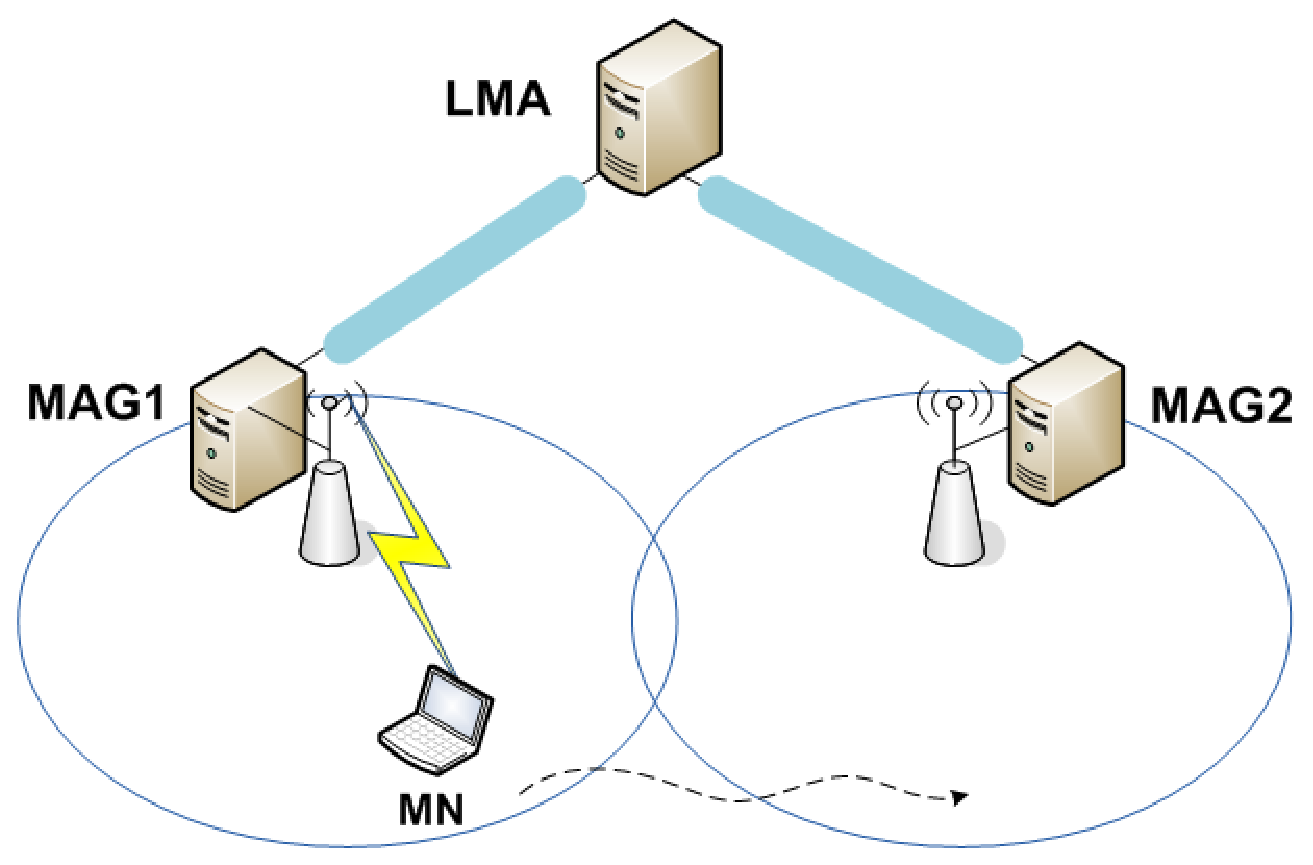
\includegraphics[width=0.50\textwidth]{./Part1/Chapter2/figures/c3_pmip_domain.eps} 
%    \caption[L'architecture d'un domaine PMIPv6]{L'achitecture d'un domaine PMIPv6.}
%     \label{fig:c3_pmip_domain}
%  \end{center} 
%\end{figure}
%
%Par rapport à MIPv6, PMIPv6 apporte certains avantages tels que: (i) évitant la complexité de la pile de protocole au MN; (ii) soutenant la mobilité sans la participation du MN; (iii) réduisant les surcharges de tunnel (sur l'air);  et (iv) diminuant la latence [73].
%
%L'opération de PMIPv6 est brièvement présentée comme suit : quand un MN entre dans un domaine PMIPv6 (attache à MAG1, par exemple), MAG1 va chercher le profil de MN (par exemple, à partir d'un serveur AAA). Puis deux messages de signalisation, le PBU et le PBA sont échangés entre MAG1 et LMA pour d'attribuer un (ou plusieurs) préfixe (s) (HNP) et mettre à jour l'emplacement actuel du MN. Un tunnel bidirectionnel est établi entre MAG1 et LMA pour rediriger le trafic de / vers le MN. Le MAG1 envoie alors un message RA, y compris l'HNP au MN. Le MN, basé sur l'HNP affecté, configure son adresse et peut l'utiliser pour communiquer avec un nœud correspondant (CN). Lorsque le MN effectue un handover de MAG1 à MAG2, le processus similaire sera exécuté pour mettre à jour l'emplacement actuel du MN au LMA. Le MAG2 obtient le même préfixe pour ce MN et peut émuler le réseau de la maison du MN (envoi des messages RA avec le même HNP). En conséquence, le MN n'est pas conscient de la mobilité et continue à utiliser la même adresse IP que précédemment.
%
%L'architecture actuelle de réseau mobile est très centralisée et hiérarchique. Ainsi les protocoles de mobilité IP (tels que PMIPv6 et DSMIPv6), qui ont été adoptés comme les protocoles de mobilité IP pour l'architecture EPC 3GPP, sont en ligne avec l'architecture centralisée et hiérarchique du réseau. Suite à l'architecture hiérarchique, les protocoles de gestion de la mobilité centralisée sont basés sur l'ancre de mobilité (HA dans MIPv6 et LMA dans PMIPv6) pour support à la mobilité. Par conséquent, à la fois le contexte de mobilité et l'encapsulation de trafic doivent être maintenus à l'ancre de mobilité. L'augmentation du nombre d'appareils mobiles et de leurs demande de trafic font des solutions de gestion de la mobilité centralisée à rencontrer plusieurs problèmes et limitations comme indiqué dans [9, 10]. Parmi eux, nous soulignons simplement les problèmes suivants :
%\begin{itemize}
%\item Le routage non optimal et le délai bout-à-bout : Lorsque le trafic de données traverse toujours l'ancre de mobilité centrale, il entraîne souvent une route plus longue. En particulier, lorsque le CN et le MN sont proches les uns des autres, mais loin de l'ancre. La même chose se produit dans le cas de CDN, dans lequel les fournisseurs de contenu mettent leurs données à la bordure du réseau. En conséquence, le délai de bout en bout sera augmenté.
%\item Le problème de l'évolutivité : La maintenance du contexte de MN et le traitement des paquets de / vers le MN nécessitent généralement des ressources de l'ancre de mobilité ainsi que les réseaux, donc réduisant l'évolutivité du système.
%\item Le gaspillage de ressources : Le service de la mobilité est toujours disponible même pour les sessions qui ne nécessitent pas le soutien de gestion de la mobilité. Ainsi, en apportant un soutien à la mobilité pour le MN/le service lorsque c'est vraiment nécessaire, les ressources de réseau peuvent être sauvées.
%\item La fiabilité: L'ancre de mobilité centrale en général constitue un goulot d'étranglement et point de défaillance unique.
%\end{itemize}
%
%La notion de DMM vise à répondre aux limites de l'approche de la mobilité centralisée soulevée quand un grand nombre d'appareils mobiles et le trafic de données sont pris en compte dans une architecture plate [9, 10]. DMM est actuellement un sujet brûlant, qui gagne beaucoup d'intérêt à la fois du monde universitaire et l'industrie. L'IETF a récemment affrété le groupe de travail DMM qui précise les solutions permettant de mettre en place des réseaux IP à l'appui d'un modèle d'ancrage distribué. Les concepts clés du DMM sont les suivants: i) les ancres de mobilité sont distribuées entre les entités de réseau et placées aussi près que possible du MN; et ii) la gestion de la mobilité est dynamique utilisée pour les sessions qui ont vraiment besoin de continuité de service. Dans DMM, une nouvelle entité est introduite - le MAR (Mobile Access Router). Cette entité peut jouer un rôle d'un HA, un LMA, un MAG ou un router normal.
%
%Dans l'approche basée sur le client, le MN est nécessaire pour participer au processus de signalisation. Chaque fois qu'un MN attache à un MAR, il obtient une adresse IPv6. Le MAR courant (cMAR) joue le rôle d'HA pour l'adresse attribuée à son réseau. Quand le MN attache au cMAR, il peut commencer une nouvelle communication avec le CN en utilisant l'adresse courante comme l'adresse de source du flux. Ce flux est acheminé de manière standard sans le mécanisme de tunnel. Lorsque le MN effectue un handover, si ce flux est encore en vie, il est acheminé via le routeur où ce flux a été initialement lancé (aMAR) en utilisant le mécanisme de tunnel entre le routeur et le MN. Pour ce faire, le MN doit mettre à jour son emplacement actuel à l'aMAR qui joue le rôle de son HA. Il est à noter que le MN doit effectuer une mise à jour de localisation pour chaque adresse IP active. En conséquence, il est nécessaire que le MN gère la liste d'HoA actifs et les aMARs associés, ainsi que la liste de sessions actives. En outre, le MN a besoin d'un mécanisme supplémentaire qui permet de sélectionner la bonne adresse IP à utiliser pour chaque session.
%
%Contrairement au DMM basé sur le client, l'approche basée sur le réseau ne nécessite pas le MN à participer au processus de signalisation. Le MAR effectue donc à la fois la fonctionnalité de LMA et de MAG. Agissant comme un MAG, le MAR détecte l'attachement du MN. Tout comme un LMA, il alloue une HNP au MN. Semblable au DMM basé sur le client, quand un MN attache à un MAR, il obtient une adresse IPv6. Typiquement, il peut utiliser l'adresse IP actuelle pour lancer des nouvelles sessions. Le trafic de données est acheminé en utilisant le routage IP normal sans aucun mécanisme de tunnelisation. Si le MN effectue un handover, le trafic sera acheminé à partir du MAR d'ancrage au MAR courant par le tunnel de la mobilité entre eux. Cependant, une question importante se pose est que la façon dont le cMAR apprend sur les adresses des aMARs. Il existe plusieurs mécanismes permettant le cMAR de connaître l'adresse des aMARs. La première méthode [90] repose sur une base de données centralisée (CMD) qui stocke les informations liées à la mobilité de chaque MN dans le domaine tel que la liste des HoAs, et l'adresse des aMARs associés comme similaire à [93]. Bien que cela permette de s'assurer que le processus de mobilité est totalement transparent pour le MN, ce mécanisme présente encore un point d'ancre centrale, cependant, pour le plan de contrôle seulement. La seconde méthode est basée sur l'information fournie par le MN comme spécifié dans [65]. En conséquence, le MN n'est plus transparent pour le processus de mobilité. Par conséquent, dans certains documents [69, 66], cette méthode est considérée comme un système basé sur le client comme indiqué ci-dessus.
%
%\subsection{Multicast IP dans le contexte de la mobilité}
%Afin de permettre le multicast IP dans MIPv6, deux approches de base ont été proposées, à savoir le tunnel bidirectionnel et la souscription à distance. Les deux approches ont leurs avantages et leurs inconvénients. Le tunnel bidirectionnel cache le déplacement des nœuds en acheminant le trafic multicast via le tunnel de mobilité entre le nœud et sa HA au prix de routage triangulaire (conduisant à un long délai) et le problème de la convergence du tunnel. D'autre part, dans l'approche de souscription à distance, le nœud multicast doit rejoindre les sessions en cours après chaque handover, ce qui pourrait mener l'interruption de service importante. En outre, des problèmes plus graves peuvent être augmentés en cas de mobilité de la source comme la transparence d'adresse et la maintien d'état de routage [11, 12]. Une amélioration supplémentaire devrait également être envisagée afin de satisfaire aux exigences supplémentaires en termes d'interruption de service et la perte de paquets pour les services en temps réel. Depuis tous ces protocoles sont conçus pour MIPv6 qui exigent les nœuds mobiles à participer au processus de signalisation, ils ne peuvent pas être appliqués directement à PMIPv6. Pourtant, l'idée de ces solutions peut être réutilisée.
%
%Comme les protocoles multicast sont conçus à l'origine pour un réseau fixe, considérant le multicast dans un environnement mobile apporte plusieurs défis au service multicast. La mobilité du nœud a des effets différents sur le service multicast, selon des facteurs tels que le rôle du nœud dans la session (source ou l'auditeur), le considéré modèle multicast (ASM ou SSM), le protocole de routage, le protocole de gestion du groupe et le protocole de mobilité en cours d'utilisation ainsi que la technologie d'accès sans fil. Par conséquent, les problèmes causé par la mobilité d'un nœud multicast peuvent être divisés en quatre groupes principaux : les problèmes généraux (en raison de protocoles multicast), les problèmes spécifiques de l'auditeur mobile, les problèmes spécifiques de la source mobile et les problèmes de déploiement [11, 12, 115]. Dans le cadre de cette thèse, nous nous concentrons sur les problèmes spécifiques de l'auditeur.
%
%La mobilité d'un auditeur provoque plusieurs problèmes pour le service multicast. Les problèmes et les solutions possibles sont décrits comme suit :
%\setlength \abovedisplayskip{-1pt}
%\vspace{-0.1in}
%\begin{itemize}
%\itemsep 0.07em
%\item L'interruption de service et la perte de paquets : Puisque le nœud mobile dans la gestion de la mobilité basée sur le réseau n'est pas au courant du processus de la mobilité, il ne peut pas prendre des décisions relatives au multicast, évitant un doux reprise de la session multicast. En conséquence, quand un auditeur se déplace à un nouveau MAG, il doit attendre pour exprimer son intérêt à s'abonner à des canaux multicast en cours jusqu'à ce qu'il reçoive une requête MLD. Ainsi, il éprouve un certain retard dans la réception de contenu multicast en raison du temps supplémentaire lié à l'activation du service multicast, la transmission MLD Query / Report (en particulier l'activation du service multicast qui est typique en quelques secondes). Ce problème devient plus grave lorsque les services en temps réel sont considérés.
%\item La duplication de paquets : Dans certains cas, le MAG peut recevoir le même paquet multicast à partir de différents LMAs ou MRs. Cela se produit lorsque différents tunnels MAG-LMA sont utilisés pour délivrer le trafic multicast.
%\item Le routage non optimal et le délai de bout en bout : Lorsque le trafic multicast doit passer par le point d'ancre de mobilité centrale (LMA), il entraîne souvent un plus long parcours. En conséquence, le délai de bout en bout sera augmenté. Ce problème devrait être prise en compte, en particulier lorsque les services en temps réel et les services sensibles au délai sont considérés.
%\item Le laisser de latence et le gaspillage des ressources de réseau : Puisque l'auditeur n'est pas conscient de la mobilité, il ne sera pas envoyer un rapport MLD pour quitter explicitement le groupe dans le MAG précédent (previous MAG - pMAG). En conséquence, si le dernier membre d'un groupe multicast se déplace à un autre MAG, le pMAG continuera d'offrir le trafic multicast jusqu'à ce qu'il met à jour ses informations des membres. Ainsi, il provoque une perte de ressources de réseau.
%\item En outre, l'auditeur peut recevoir le paquet hors de l'ordre en raison de handover. Dans de nombreux régimes sans fil, la signalisation liée au multicast doit être minimisée pour réduire la consommation d'énergie (avec la capacité limitée) et la ressource de réseau en cours d'utilisation. Encore une fois, l'ajustement des paramètres MLD [115] doit être soigneusement étudié comme un compromis des surcharges de signalisation et de l'interruption de service.
%\end{itemize}
%
%\paragraph{Les solutions en point de vue de l'IETF}
%
%Suite à une architecture typique de déploiement, le support multicast peut être activé en déployant le proxy MLD et la fonction de MR dans le domaine. En général, les différentes propositions sont issues en correspondant de l'emplacement de MAG et LMA dans l'architecture de déploiement de multicast. En conséquence, il existe deux approches principales correspondant aux différents rôles de MAG et LMA comme : i) MAG agit comme un proxy MLD tandis que LMA agit comme un MR ou un proxy supplémentaire; et ii) MAG et LMA jouent le rôle d'un MR. La première approche est considérée comme une solution de base par l'IETF. Cette solution peut également être considérée comme une solution basée sur le mécanisme de tunnelisation en raison du fait que le trafic multicast est routé via le tunnel de mobilité entre LMA et MAG. Dans la seconde approche, par le déploiement de routage multicast à MAG, plusieurs problèmes peuvent être évités (par exemple, le routage sous-optimal, problème de convergence) à un coût de fonctionnement et de déploiement du router multicast.
%
%\paragraph{La solution de base}
%La solution de base, qui a été normalisée par l'IETF, offre le soutien de la mobilité de l'auditeur dans PMIPv6 en plaçant la fonction proxy MLD au MAG, tandis que le LMA agissant comme un MR ou un proxy supplémentaire. La fonction proxy MLD est mise en œuvre au MAG avec l'interface « en amont » étant configuré vers le LMA. Comme une opération typique du proxy MLD, les données arrivant d'une interface « en amont » seront transmises aux interfaces « en aval » qui ont états appropriés pour ce groupe. Ainsi, tout le trafic multicast passe par le tunnel MAG-LMA, comme le trafic unicast. Après chaque handover, le trafic multicast continue de fournir à l'auditeur dans le nouveau MAG, et la continuité de service est assurée en conséquence. En outre, du point de vue de service multicast, l'auditeur ne connaît pas la mobilité. Il est atteint puisque le nouveau MAG, après l'obtention d'informations sur l'abonnement de l'auditeur en utilisant les opérations normales de MLD, rejoint les flux multicast courants de la part de l'auditeur. La solution de base peut être également appliquée à la source multicast [118].
%
%Lorsqu'un MN est attaché à un MAG (MAG1), après l'exécution des opérations PIMPv6 standards, MAG1 crée une instance proxy MLD (si nécessaire), qui sert comme un routeur « en amont » de tous les nœuds associés du LMA du MN. Cette instance ajoute le MN à son interface « en aval » et configure son interface « en amont » vers le LMA du MN. Lorsque le MN exprime sa volonté de recevoir le trafic multicast d'un groupe, il envoie un rapport MLD à MAG1. Le MAG1 envoie alors un rapport agrégé au LMA à rejoindre le groupe au nom du MN. Le LMA, agissant comme un MR, rejoint le groupe de l'infrastructure multicast, et met à jour son état de transmission. Après avoir reçu les paquets multicast, le LMA les transmet aux MAGs appropriées (via le tunnel LMA-MAG) en fonction de son état de transmission. Le MAG1 transmet ensuite les paquets aux interfaces appropriées « en aval » et ils ont finalement atteint le MN. En cas de handover (de MAG1 à MAG2), puisque la mobilité est transparente pour le MN, le MN ne sera pas envoyer les rapports MLD non sollicités. Au lieu de cela, MAG2, lors de la détection d'un nouveau MN sur la liaison d'accès, ajoute le MN à une interface « en aval », et envoie des messages MLD de requête générale sur sa liaison attachée. Le MN répond alors par un message MLD y compris les états actuels des groupes multicast. Sur cette base, MAG2 peut rejoindre les groupes au nom du MN. Les paquets multicast sont acheminés depuis LMA à MAG2 et atteignent finalement le MN.
%
%Bien que la solution de base soit un moyen très simple pour activer le support multicast dans PMIPv6, il ne traite pas des problèmes liés à la mobilité multicast. Dans plus de détails, l'utilisation de tunnel pour les flux multicast provoque la redondance du trafic (ou le problème de la convergence) au MAG. C'est parce que les différents nœuds, qui sont attachés au MAG et associés à différents LMAs peuvent s'abonner pour le même groupe. En outre, depuis plusieurs opérations doivent être exécutées pour permettre le MN continuer à recevoir le trafic multicast au nouveau MAG, il peut provoquer une longue interruption de service et un grand nombre de perte de paquets. En outre, comme le trafic multicast passe toujours par le LMA, il peut provoquer le problème de routage sous-optimal.
%
%\subsection{La mobilité d'un nœud multicast dans un domaine DMM orienté réseau}
%\begin{figure}[h!] 
% \begin{center} 
% 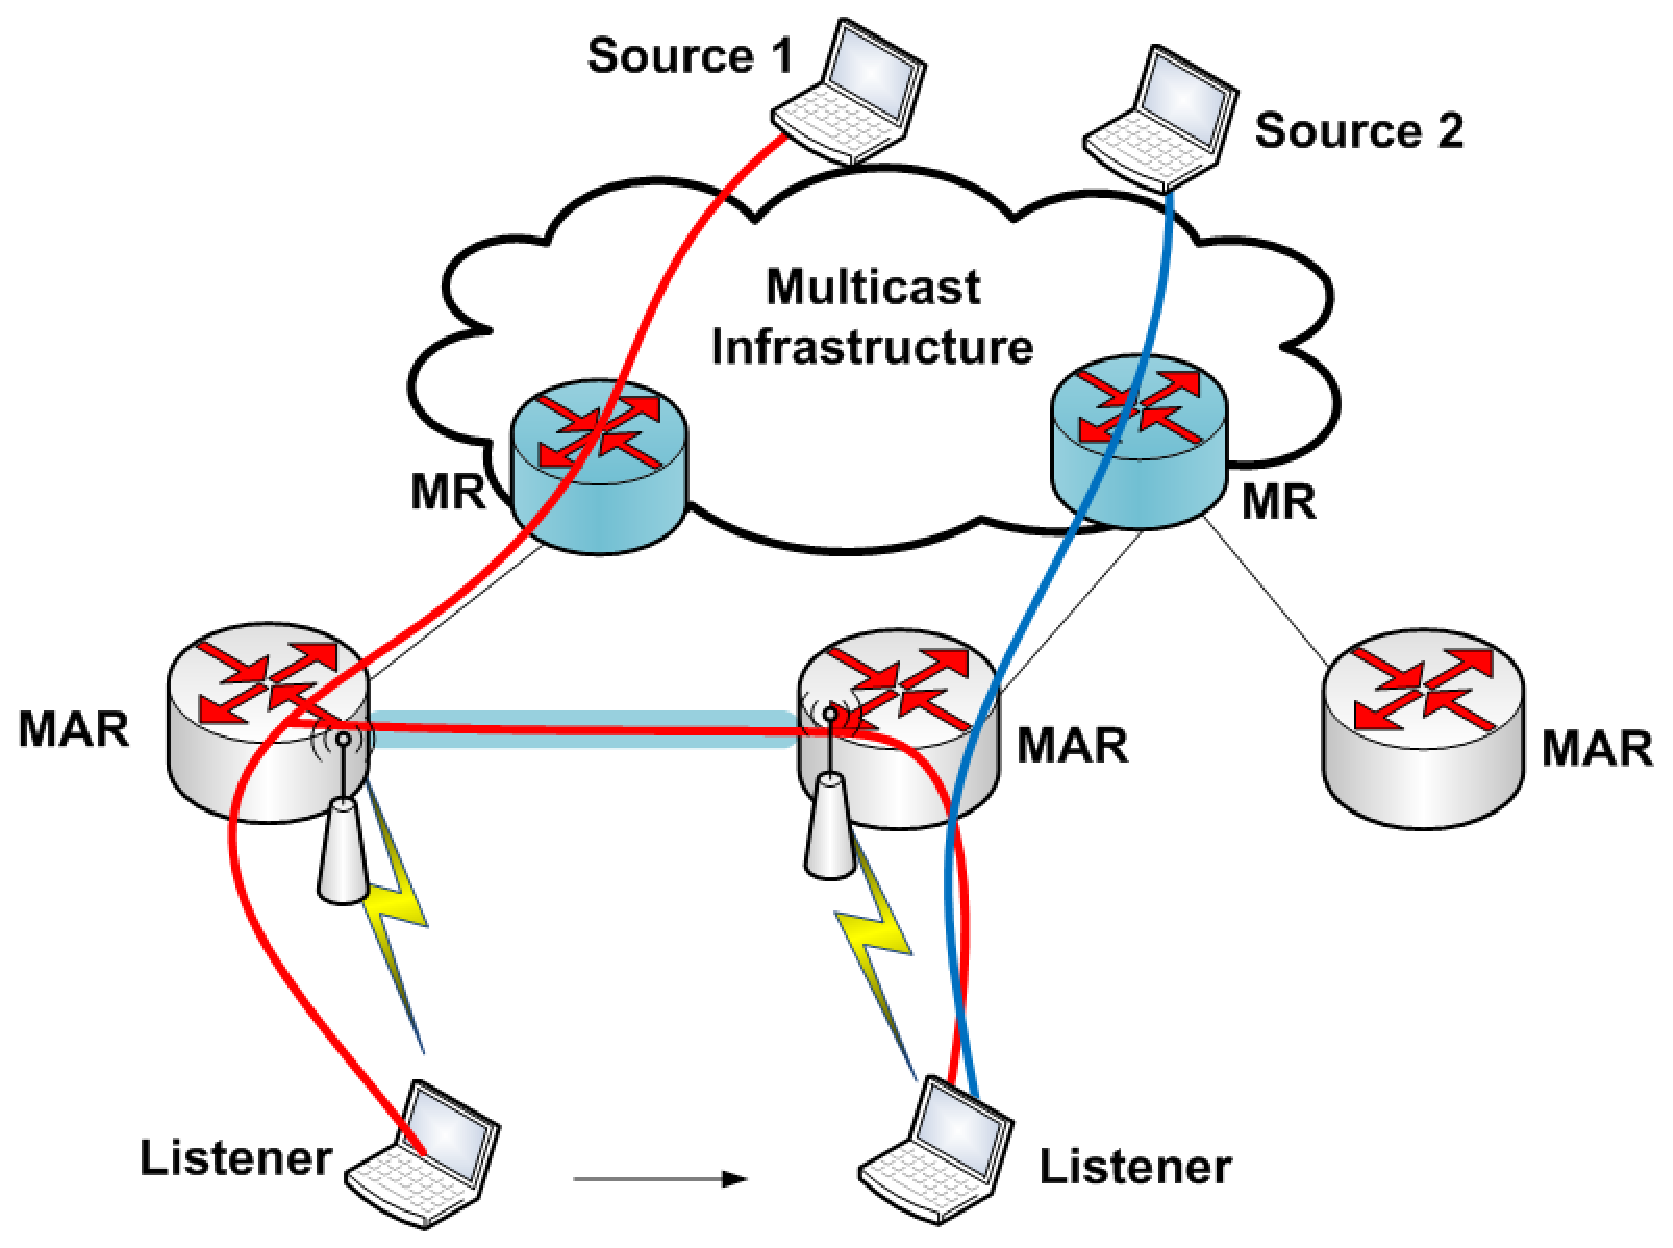
\includegraphics[width=0.50\textwidth]{./Part1/Chapter2/figures/c4_dmm_listener_mld.eps} 
%    \caption{La mobilité d'un auditeur dans un environnement DMM (la fonction de proxy MLD est déployée à MARs).}
%     \label{fig:c4_dmm_listener_mld}
%  \end{center} 
%\end{figure}
%
%Puisque DMM est encore à un stade précoce de la normalisation, il y a un travail limité pour le soutien au multicast. Jusqu'à présent, aucune solution complète n’a été trouvée pour le multicast dans DMM. En règle générale, tous les principaux aspects sont hérités du problème dans un domaine PMIPv6, tandis qu'une complexité supplémentaire est ajoutée. Il est à noter que cette section ne présente que les problèmes et les solutions en considérant un environnement DMM orienté réseau.
%
%Comme dans PMIPv6, le soutien à la mobilité de l'auditeur multicast peut être activé dans DMM en déployant le proxy MLD à MAR [128, 22, 20]. Dans ce cas, quand un flux multicast est lancé, le trafic multicast est reçu directement à partir de l'infrastructure multicast native via le MAR courant. Dans le cas du handover, le trafic est acheminé à partir de MAR d'ancrage au MAR courant via le tunnel entre eux (comme le trafic d'unicast). Cependant, ce mode ne traite pas des problèmes relatifs au multicast. Parmi eux, nous soulignons seulement les problèmes y compris l'interruption de service, le routage non-optimal, le délai de bout en bout, et le problème de la convergence, et la perte de paquets. 
%
%Considérant le déploiement de la fonction MR à MARs, le MAR décidera le trafic multicast d'un MR pour un auditeur attaché basé sur le Reverse Path Forwarding (RPF). Par conséquent, la convergence du tunnel et le routage non-optimal seront évités. Cependant, le mouvement de l'auditeur provoque le problème de l'interruption de service. En outre, les opérateurs ne veulent pas déployer la fonction de routage multicast sur le MAR en raison de sa mise en œuvre et le coût d'exploitation par rapport à proxy MLD.
%
%\subsection{Evaluation de la performance}
%\subsubsection{Métriques pour l'évaluation de la performance}
%Pour évaluer la performance d'un protocole de gestion de la mobilité, un ensemble de paramètres est en général considéré incluant le coût de signalisation, le temps de handover (temps de latence), le délai de bout en bout et le coût de tunnelisation. Le coût de signalisation est défini comme le coût de mettre à jour l'emplacement du MN. Il est un facteur important car il influence l'évolutivité du système ainsi que le coût de livraison de données, en particulier lorsqu'on considère environnement sans fil qui a typiquement une capacité limitée. En ce qui concerne le temps de latence, il est définie comme une période où un nœud ne peut pas recevoir / envoyer des paquets en effectuant un handover. C'est le temps écoulé entre le dernier paquet reçu via l'ancien routeur et l'arrivée du premier paquet via le nouveau routeur après un handover. Au cours de cette période, les paquets sont perdus. Ainsi, il peut entraîner de l'interruption notable de service, surtout dans le cas d'applications sensibles au délai comme la vidéo et la voix sur IP (VoIP). Le nombre de paquets perdus est généralement proportionnel à la latence de handover. Dans les réseaux basés sur IPv6, QoS peut être définie par la perte de paquets, la latence et les surcharges de signalisation [72]. En conséquence, une longue période de latence et un grand nombre de paquets perdus peuvent dégrader la qualité du service. Par conséquent, la réduction du temps de latence et de la perte de paquets améliore la performance de l'application. D'autre part, le délai de bout en bout entre deux nœuds est la somme des retards rencontrés au long du trajet entre ces nœuds. En général, le délai de bout-en-bout comprend non seulement le délai de la transmission sur les liens, mais également la mise en attente de traitement et de retard au niveau des nœuds intermédiaires [133]. Des nombreuses applications populaires de multimédia (par exemple, le jeu en temps réel, le streaming vidéo en direct et VoIP / Vidéo conversationnel) ont de délai strict.
%\begin{figure}[h!] 
% \begin{center} 
% 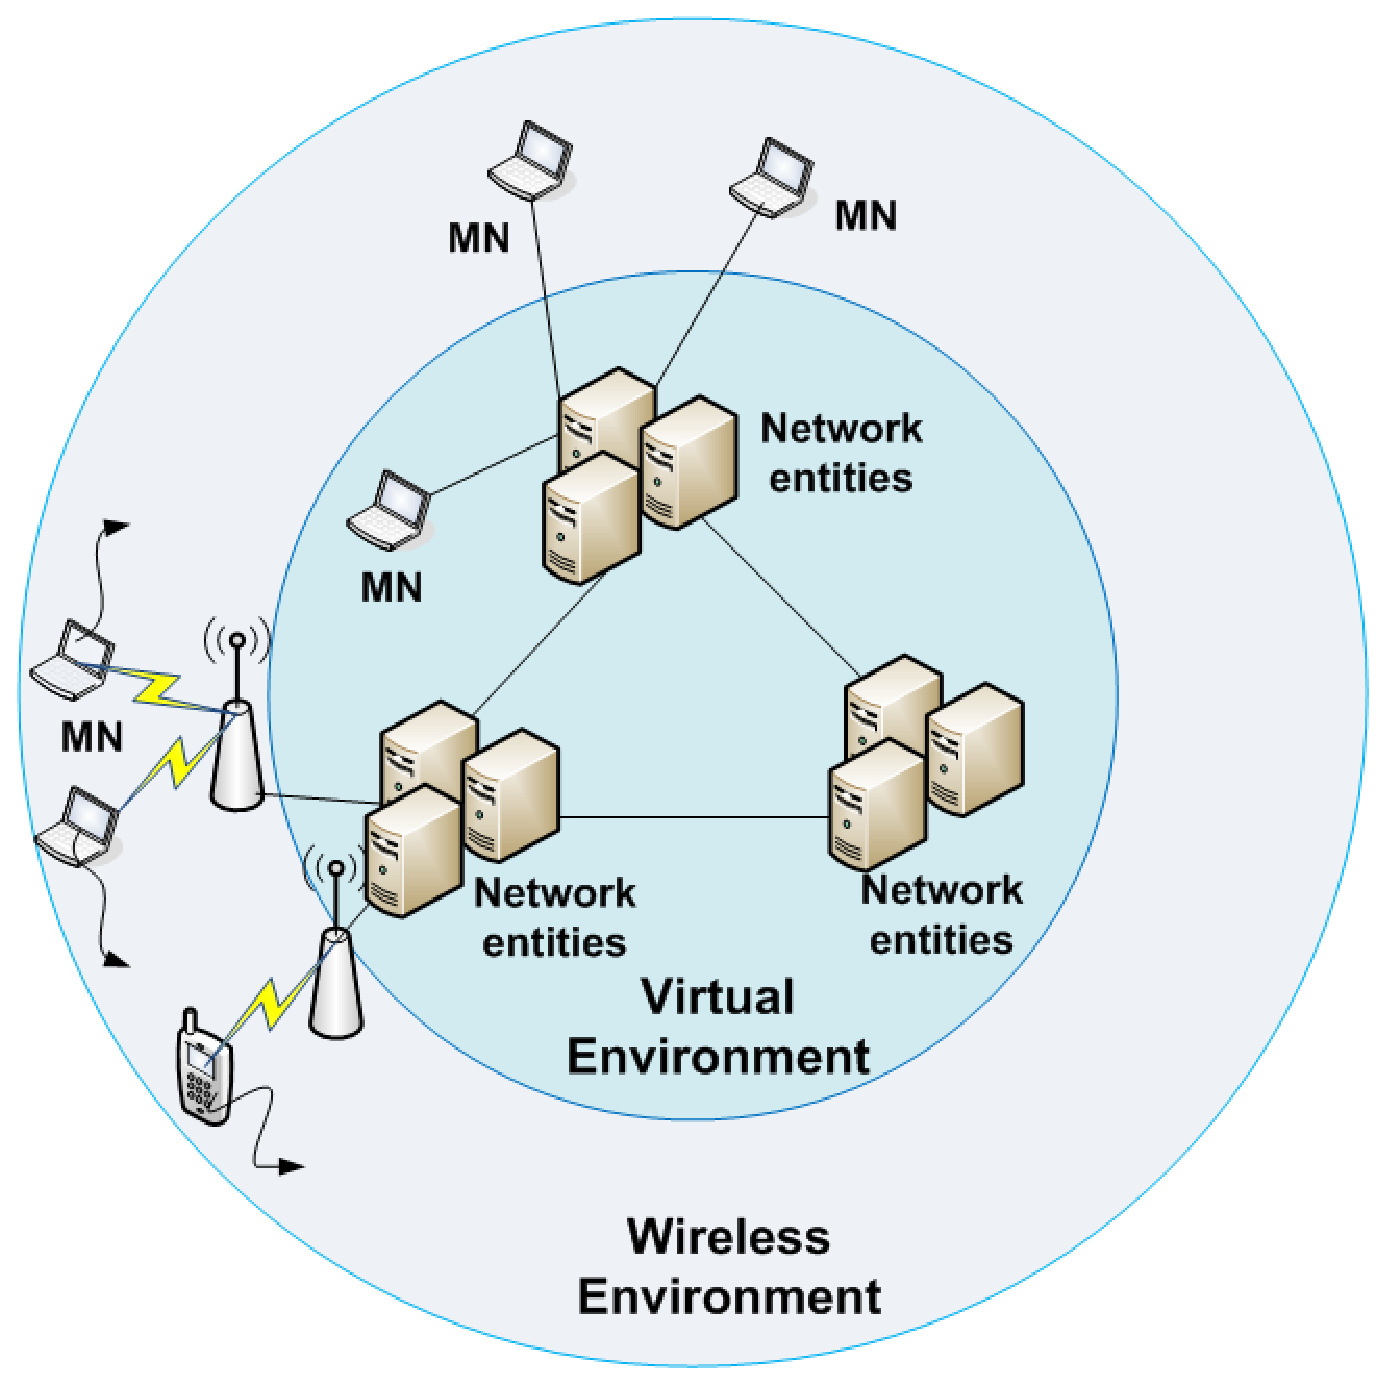
\includegraphics[width=0.45\textwidth]{./Part1/Chapter3/figures/c5_architecture.eps} 
%    \caption{L'architecture d'un banc d'essai proche de réel.}
%     \label{fig:c5_architecture}
%  \end{center} 
%\end{figure}
%
%\subsubsection{Evaluation expérimentale pour les réseaux sans fil}
%Dans la recherche en réseau, il y a des diverses méthodes d'expérimentation, tels que : le banc d'essai réel, la simulation, l'émulation, la virtualisation et la modélisation mathématique (ou théorique). Chaque méthode a ses avantages et ses limites [135]. L'utilisation d'un banc d'essai réel est considérée comme la meilleure méthode expérimentale. Cependant, elle implique un coût plus élevé de déploiement et manque d'évolutivité. Bien que la simulation soit très populaire grâce à sa flexibilité et facile à déployer des fonctionnalités, les résultats obtenus dans certains cas, ne sont pas fiables. L'émulation peut être considérée comme un compromis entre la simulation et un banc d'essai réel apportant des résultats plus précis (par rapport à la simulation) et à moindre coût (par rapport au banc d'essai réel). Pourtant, l'émulation a des limites sur le déploiement et l'évolutivité, qui peuvent être atténués en utilisant la technique de virtualisation. Enfin, la modélisation mathématique est parfois utilisée, mais seulement d'une façon simplifiée, en faisant abstraction de la complexité. En outre, pour aider à justifier notre approche sur la méthode expérimentale, nous devons mentionner que notre étude concerne les environnements mobiles et nous devons donc garder à l'esprit les exigences les plus importantes que d'une méthode expérimentale doit se concentrer sur sont la précision, la fiabilité, la mobilité et l'évolutivité [136 ].
%
%Dans cette thèse, nous introduisons un environnement d'expérimentation proche du réel qui se compose d'un environnement de virtualisation et simulation. La première partie peut être considérée comme l'infrastructure du réseau dans lequel les multiples machines virtuelles sont reliées, tandis que la seconde partie est un réseau d'accès sans fil essentiellement composé par le simulateur NS-3. En combinant ces éléments, nous avons produit une méthode qui peut atteindre un niveau supérieur de réalisme en conservant les avantages de la méthode de simulation et encore être en mesure d'exécuter des logiciels et des protocoles réels. Puisque cet environnement est un open-source et facile à déployer, il peut être réutilisé par d'autres chercheurs à créer leur propre environnement d'expérimentation. De plus, il permet la conception et l'évaluation du réseau de taille petit à moyenne et de déployer les protocoles dont les résultats peuvent être facilement convertis dans le monde réel. En particulier, cette méthode est appropriée pour les cas suivants : i) l'infrastructure fixe; ii) la mobilité et les réseaux mobiles; iii) l'expérimentation de la couche supérieure à la couche réseau (par exemple, la gestion de la mobilité, le multicast, les applications, etc.); iv)  l'infrastructure du réseau de taille moyenne; et v) le réseau de taille grande en fonction de nœuds mobiles.
%
%\vspace{-0.22in}
%\section{La mobilité d'un nœud multicast dans PMIPv6}
%\subsection{Optimisation de la continuité de service dans un domaine PMIPv6}
%
%La solution de base a été récemment adoptée pour soutenir la mobilité de l'auditeur dans PMIPv6. Néanmoins, elle ne traite pas des problèmes d'optimisation et de performance tels que le temps d'interruption de service, les surcharges de tunnel, et le routage non optimal, etc. En ce qui concerne le temps d'interruption de service, nous proposons une méthode basée sur la combinaison des mécanismes de transfert de contexte multicast et de fonction de suivi explicite pour minimiser le temps d'interruption. Commençant par l'analyse du temps de l'interruption, les expériences sont ensuite effectués pour comparer différentes approches reposant sur un banc d'essai près au réel. Les résultats numériques et expérimentaux montrent que grâce à l'utilisation de transfert de contexte multicast, le temps d'interruption peut être réduit de manière significative. En ajustant le comportement du MLD pour les routeurs, nous pouvons également obtenir un résultat similaire, mais arrive une dramatique augmentation de la signalisation liée au multicast. Particulièrement, le problème sera plus grave avec un grand nombre d'auditeurs. En outre, grâce au transfert de contexte multicast le temps de congés (leave latency) est minimisé. Par conséquent, le protocole de transfert de contexte en général peut être considéré dans les solutions proposées. A noter que la fonction de transfert de contexte et la fonction de suivi explicite mises en œuvre peuvent être utilisées dans notre banc d'essai, ainsi que dans un vrai banc d'essai. Notre banc d'essai peut être servi comme un banc d'essai proche du réel, qui peut fournir des résultats réalistes à faible coût pour l'expérimentation de la mobilité multicast dans un domaine PMIPv6.
%\begin{figure}[h!] 
% \begin{center} 
% 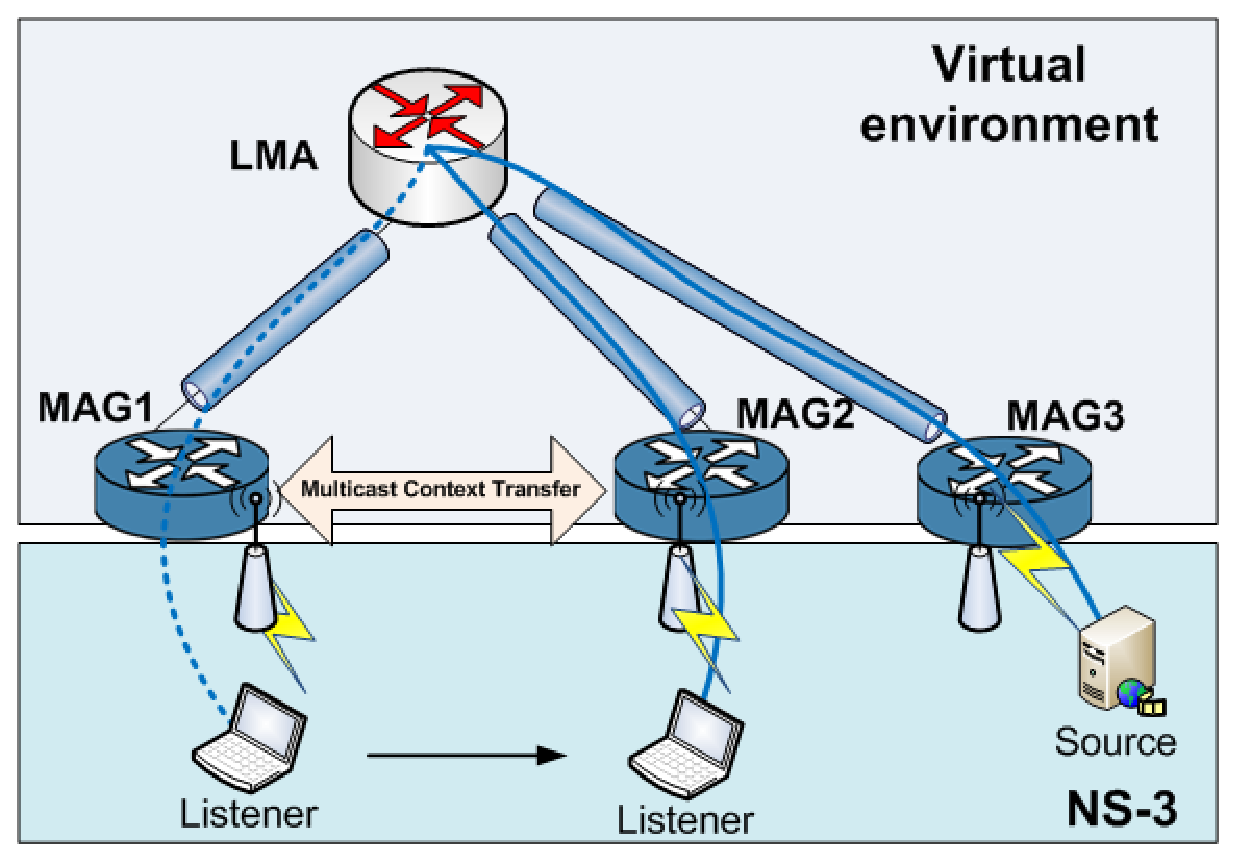
\includegraphics[width=0.53\textwidth]{./Part2/Chapter4/figures/optimizing.eps} 
%    \caption{Le déploiement d'un banc d'essai proche au réel.}
%     \label{fig:c5_architecture}
%  \end{center} 
%\end{figure}
%
%Pour réduire le temps d'interruption, l'objectif est de réduire le temps nécessaire au nouveau MAG (nMAG) pour obtenir des informations d'abonnement multicast actives du MN pendant handover. Alors que le nMAG peut s'abonner à des flux courants (à l'avance) et transmet les paquets multicast au MN dès que possible. Pour ce faire, des informations  d'abonnement sont échangées entre le pMAG et le nMAG. En outre, cette solution est indépendante de la technologie de la couche 2 et plus facile à déployer que les propositions existantes. Le transfert de contexte multicast est également mis au point conformément à la norme pour le protocole de transfert de contexte [159]. En outre, la solution proposée ne met pas de charge supplémentaire sur le LMA, ce qui rend notre solution meilleure en comparaison avec la solution M-LMA en termes d'évolutivité.
%
%\subsection{Equilibrage de charge du flux multicast dans les réseaux PMIPv6 }
%La croissante de la pénétration des appareils mobiles, tels que les tablettes et les téléphones intelligents génère un grand nombre de trafic de données, en particulier le trafic vidéo sur les réseaux mobiles [6, 1]. Dans ce contexte, il est fréquent d'avoir un grand nombre de périphériques associés au LMA dans un domaine PMIPv6 donc facilement faire le LMA un goulot d'étranglement et un point de défaillance unique. Par conséquent, la qualité des sessions en cours pourrait être dégradée (par exemple, une augmentation du délai de la file d'attente et une augmentation du perte de paquets). En conséquence, les opérateurs des réseaux mobiles peuvent avoir besoin de déployer plusieurs LMAs dans un grand domaine PMIPv6, de sorte que le trafic peut être réparti entre les LMAs [76]. Pourtant, il est fort possible que certains LMAs deviennent surchargés alors que les autres sont sous-utilisés. Par conséquent, l'équilibrage de charge (LB) entre les LMAs est nécessaire. Du fait que le multicast IP devrait être largement déployé dans un proche avenir pour faire face à une énorme demande de trafic multimédia. Ainsi que, le contenu de la vidéo mobile a généralement des débits beaucoup plus élevés que les autres types de contenu. Le service multicast devrait donc jouer un facteur crucial dans la mise charge sur le LMA. Cependant, son rôle a été négligé dans toutes les propositions existantes. Par conséquent, l'utilisation de service multicast dans les mécanismes LB existants peut conduire à plusieurs problèmes à la fois de LB (la dégradation de l'efficacité) et de service multicast (par exemple, le problème de la convergence et  l'interruption de service).
%
%Pour ces raisons, nous introduisons un mécanisme d'équilibrage de charge (en fonction de multicast), qui prend le service multicast en compte. L'idée clé est que par la séparation du mécanisme d'équilibrage de charge multicast à partir de l'unicast, la solution proposée permet de mieux répartir la charge entre les LMAs dans runtime, ainsi que d'améliorer l'efficacité de l'utilisation des ressources.
%
%Dans plus de détails, deux approches différentes, à savoir l'approche proactive multicast (ou MAG-initié) et  l'approche réactive multicast (ou LMA-initié) sont considérées. Dans le premier cas, le mécanisme LB sera appelé lorsqu'un MN démarre une nouvelle session multicast pour sélectionner un LMA approprié à servir cette session. Dans ce dernier cas, le mécanisme LB sera exécuté quand un LMA est surchargé en sélectionnant une session de multicast pour passer à un LMA moins chargée. Il peut être fait grâce à une extension de proxy MLD pour supporter de multiples interfaces « en amont » [167]. Dans ce cas, une seule instance de proxy est déployée à MAG avec plusieurs interfaces « en amont » étant configurées vers différents LMAs. En conséquence, le MN peut recevoir le trafic multicast à partir d'un LMA moins chargé, en obtenant le trafic unicast à partir de sa LMA. Par conséquent, la solution proposée ne modifie pas les sessions multicast/unicast en cours.
%
%\subsection{Mobilité dans les réseaux hétérogènes}
%La mobilité dans les réseaux hétérogènes sera illustrée via un cas d'utilisations: le service de recharge de véhicule électrique (EVCS). Il y a plusieurs raisons pour choisir ce cas d'utilisation. Tout d'abord, le véhicule électrique (EV) est un choix prometteur pour le transport personnel dans un proche avenir. Deuxièmement, l'idée de connexion des véhicules prend de l'ampleur. En outre, un nœud mobile (ou un véhicule électrique dans ce contexte) peut être relié à l'infrastructure via différentes technologies sans fil / filaires dans différentes étapes. Ainsi, compte tenu multicast dans le véhicule électrique est une étape pour permettre de déployer système de divertissement à l'EV, qui devient de plus en plus populaire. En outre, le multicast IP peut également être utilisé pour mettre à jour le logiciel des systèmes embarqués.
%
%\begin{figure}[h!] 
% \begin{center} 
% \includegraphics[width=0.80\textwidth]{./Part2/Chapter6/figures/c8_use_cases.eps} 
%    \caption{Les cas d'utilisation de service EVCS.}
%     \label{fig:c5_architecture}
%  \end{center} 
%\end{figure}
%
%Comme indiqué dans [184], la condition essentielle pour obtenir des avantages énergétiques et économiques de Smart-Grid et de véhicules électriques est d'atteindre un ordonnancement optimal de la charge des véhicules électriques et le stockage de l'électricité par les EVs. Ainsi, il est important pour les opérateurs du Grid de surveiller les données nécessaires (comme la consommation d'énergie et la demande) et d'attribuer et de router des véhicules vers les stations de recharge appropriées pour appuyer leurs politiques de tarification nécessaires. Cette négociation ne peut être menée à la station de charge, mais doit être effectuée pendant la conduite. L'EV doit donc communiquer avec l'infrastructure de charge [185]. Dans ce contexte, plusieurs technologies d'accès (par exemple, WLAN, LTE, et PLC) doivent être utilisés lors des différentes phases de l'EVCS, comme LTE pendant la conduite, WLAN en approchant une station de charge, et PLC en étant amarré à une station de recharge. Ces technologies de communications hétérogènes doivent être transparentes pour l'utilisateur, la gestion de réseau et pour l'EVCS afin de maintenir le contexte de service.
%
%Nous vous proposons une solution de EVCS à la fois point de vue de l'utilisateur et de l'opérateur de Grid. Pour l'utilisateur, il offre un service omniprésent et  transparent à différents scénarios (à la maison, à une station de charge et à un parking), ce qui rend le chargement d'un EV aussi simple que possible. Il contribue également à l'operateur du réseau de gérer efficacement la consommation de l'utilisateur et la demande sur le Grid, surtout quand un grand nombre de véhicules électriques est considéré. De la nature centralisée de service de Smart-Grid, une solution de la gestion de la mobilité centralisée basée sur le réseau, par exemple, PMIPv6 est le plus appropriée pour fédérer les services de charge segmentés et faire l'expérience de charge transparente de la mobilité des EVs ainsi que la technologie de communication utilisée par chaque phase du EVCS. En utilisant PMIPv6, le service prend en charge la mobilité des EVs, les handovers verticaux et horizontaux entre les différentes technologies de communication. Pourtant, la conservation de l'adresse IPv6 dans PMIPv6 reste un problème dans un tel contexte, et nous fournissons une solution en s'appuyant sur une approche de l'interface logique pour cacher la modification de l'interface vers la pile IPv6 (du point de vue de la couche IP). Le concept d'EVCS et la performance du PMIPv6 pour l'EVCS ont été validés à l'encontre de référence de la norme IEEE 1646. Un banc d'essai proche au réel, qui est une combinaison des machines réelles et virtuelles, a été déployé pour réduire le coût du matériel et de fournir d'expérience flexible. Un lien réel PLC fournis par les partenaires du projet VELCRI est utilisé pour obtenir des résultats réalistes.
%
%\subsection{La mobilité inter-domaine : du point de vue du DMM}
%Comme mentionné précédemment, en profitant de la gestion de la mobilité basée sur le réseau, PMIPv6 permet à la mobilité IP pour déplacer les clients sans leur participation. PMIPv6 apporte plusieurs avantages par rapport à la gestion de la mobilité basée sur le client comme MIPv6. Cependant, PMIPv6 échoue à soutenir la mobilité inter-domaine. Cela signifie que, même si un MN se déplace vers un autre domaine PMIPv6, la continuité de la session ne peut être maintenue.
%
%Afin de soutenir la mobilité inter-domaine, plusieurs solutions ont été proposées, par exemple, l'intégration de MIPv6 et  PMIPv6 (H-PMIP) [192]; et  I-PMIP [193]. Pourtant, elles ont des limitations telles que le routage sous-optimal, les surcharges de signalisation et la latence de handover. Surtout, en raison du manque de granularité sur le service de gestion de la mobilité, la mobilité est toujours disponible même pour les sessions qui ne nécessitent pas de support de gestion de la mobilité (par exemple, les sessions qui sont lancées et terminées alors que le nœud mobile connecté au même domaine).
%
%Basé sur le concept DMM, nous introduisons un support à la mobilité inter-domaine, appelé D-PMIP. Ainsi, cette proposition apporte certains avantages : (i) les ancres de mobilité sont placées près de MN; et  (ii) le service de la mobilité n'est disponible que pour les sessions qui nécessitent vraiment la continuité du service. Une fois que le MN entre son domaine PMIPv6, il obtient un préfixe. Basé sur le préfixe attribué, le MN configure son adresse IPv6. Le MN peut ensuite utiliser cette adresse pour initier et maintenir les sessions de façon standard alors qu'il reste attaché à ce domaine. Lorsque le MN change son domaine, il obtient un autre préfixe et configure une nouvelle adresse basée sur ce préfixe. Cette adresse peut être utilisée pour mettre en place les nouvelles sessions. Jusqu'à ce que les sessions précédentes ne soient pas fermées, les anciennes adresses doivent être maintenues. Ainsi, un tunnel est construit entre le LMA d'ancrage et le LMA actuel à rediriger les paquets entre deux LMAs.
%
%Basé sur le concept DMM, deux solutions possibles pour la mobilité inter-domaine sont considérées, à savoir la solution de partie distribuée (DP-PMIP) et la solution d'entier distribuée (DF-PMIP). La première solution repose sur une base de données commune pour le plan de contrôle, alors que dans la dernière la fonction de la mobilité est répartie dans les deux plans : le plan de contrôle et le plan de données. Ainsi, deux solutions permettent à des paquets de données à être acheminés via une manière quasi-optimale en mettant les points d'ancrage de mobilité plus proche du MN tandis que le plan de contrôle peut être placé n'importe où dans le réseau. Les résultats numériques montrent que la solution DP-PMIP donne des meilleures performances que les solutions existantes (par exemple, MIPv6, H-PMIP et I-PMIP) en termes de latence, de coût de signalisation et d'utilisation du tunnel.
%\section{La mobilité d'un nœud multicast dans DMM}
%
%Comme indiqué précédemment, le multicast IP peut être activé dans DMM en déployant la fonction proxy MLD à MAR. Pour le nouveau flux, le trafic multicast est transmis directement à partir de l'infrastructure multicast via le MAR courant. Pour le flux après le handover, le trafic est tunnelé du MAR où le flux est initié au MAR courant par le tunnel de la mobilité entre eux. Ainsi, le point d'ancre de mobilité multicast (MMA) est associé à la phase initiale du flux multicast (identique à l'ancre de mobilité unicast) : le MAR où le flux est initiée. Le flux multicast sera ancré au MMA initialement attribué au cours de sa vie. Par conséquent, même lorsque le MN se déplace loin de son point d'ancre, le trafic de multicast traverse encore l'ancre. En conséquence, il provoque plusieurs problèmes au flux multicast en cours, comme l'interruption de service, le routage non-optimal, le délai de bout-en-bout et la duplication de paquets. Ces problèmes deviennent graves lorsqu'on considère les services sensibles à l'interruption et aux délais. En outre, même les ancres de mobilité sont distribuées, des ancres sont plus surchargées que les autres \cite {anchor_selection}.
%
%Dans cette section, nous soutenons principalement la nécessité d'un mécanisme de sélection dynamique de l'ancre de mobilité multicast (DMMA). D'un point de vue du service, il contribue à satisfaire les exigences en termes de l'interruption du service et le délai, en particulier lorsqu'on considère les services en temps réel. Il fournit un mécanisme permettant de mieux répartir la charge entre MARs. En outre, d'autres problèmes telles que la duplication de paquets et le laisser latence (perte de ressources) peuvent être réduits. Le DMMA prend en compte non seulement le contexte du service, mais aussi le contexte de la mobilité du nœud et le contexte du réseau, permettant un support par flux. En d'autres termes, chaque flux multicast peut être traité différemment selon différents contextes.
%
%\subsection{La mobilité de l'auditeur dans DMM} \label{c10:multicast_listener}
%
%En ce qui concerne l'interruption de service, quand un auditeur multicast se déplace de pMAR à cMAR, il peut provoquer une interruption de service perceptible pour les flux en cours. En conséquence, le transfert de contexte multicast est nécessaire pour éviter une grande interruption causée par les procédures relatives au service multicast (environ 5 s dans le cas normal, et de 2,5 s dans le meilleur des cas) \cite{Thinh_WCNC_Multicast}. Ce délai est beaucoup plus long que le temps d'interruption de tolérance maximum pour les services normaux, comme spécifié dans \cite{interruption_requirements} est de 500 ms. Même avec le transfert de contexte, il est incapable de répondre à l'exigence en termes d'interruption pour le service sensible à l'interruption lorsque le délai cMAR-aMAR est grand \cite{Thinh_ICNS,multicast_DMM_Sergio_PIMRC}. C'est parce que le trafic multicast doit passer par l'aMAR, qui joue le rôle de point d'ancrage de multicast (MMA). En outre, puisque le trafic de multicast traverse toujours l'aMAR, il entraîne souvent une route plus longue. Particulièrement, considérant un grand domaine, il peut provoquer un délai de bout en bout élevé. Ce problème devient plus sérieux lorsque le service sensible au délai est considéré.
%
%
%En cas de mobilité, l'utilisation du tunnel pour le flux multicast peut entraîner le problème de la convergence. Puisque le but de DMM est de déplacer les ancres de mobilité du coeur vers la périphérie du réseau, le nombre de points d'ancrage dans un domaine DMM sera beaucoup plus que celui dans un domaine PMIPv6. En conséquence, le problème de la convergence est supposé être bien plus sévère que celui dans PMIPv6. En utilisant une extension de proxy MLD pour supporter de multiples interfaces « en amont » \cite{multiple_upstreams}, le problème de la convergence peut être évité. 
%
%\begin{figure}[tb!] 
%  \begin{center} 
%    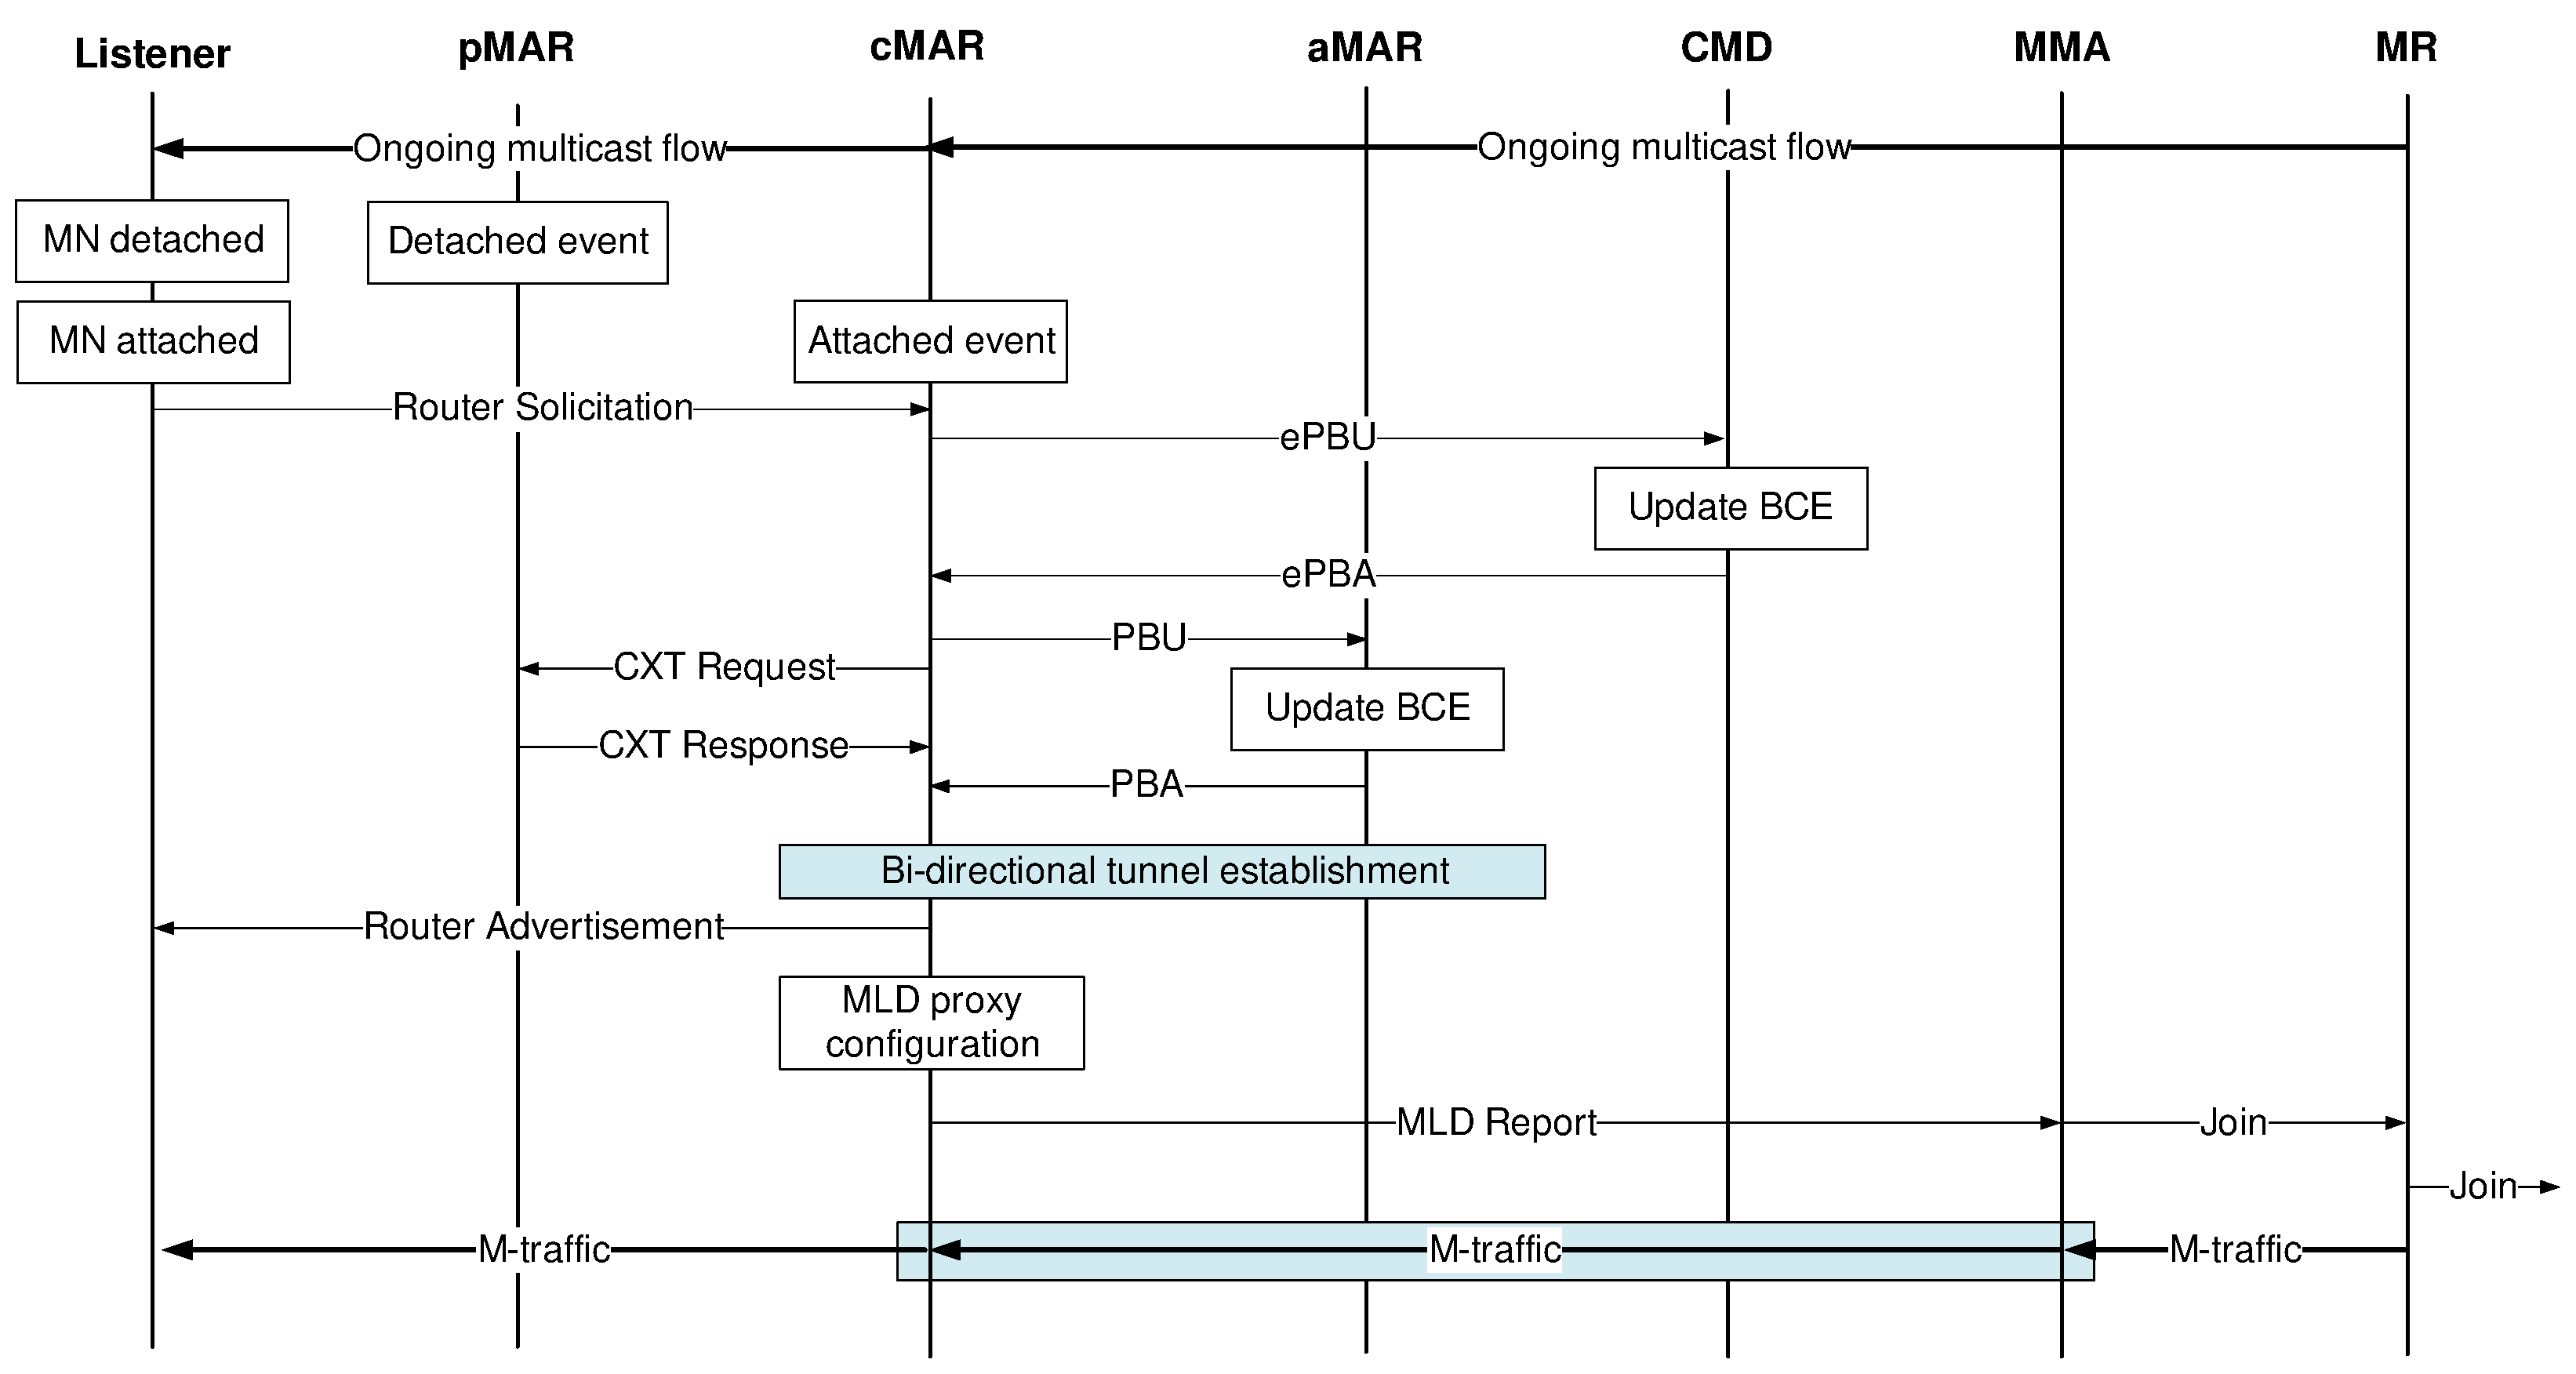
\includegraphics[width=0.90\textwidth]{./Part3/Chapter8/figures/c10_service_disruption_common.eps} 
%    \caption[La signalisation quand un auditeur exécute un handover.]{La signalisation quand un auditeur exécute un handover.}
%    \label{fig:c10_HO}
%  \end{center} 
%\end{figure}
%
%Pour souligner ces problèmes, nous considérons différents candidats pour le MMA comme l'aMAR (le mode par défaut), le pMAR, le cMAR (le subscription native), ou un MMA commun (COMMA) qui sert comme un seul MMA pour le domaine (comme dans \cite{direct_routing_mtma}). Différentes approches MMA\_aMAR, MMA\_pMAR, MMA\_cMAR et MMA\_COMMA sont considérées, en conséquence. Nous considérons également l'impact du déploiement de proxy MLD avec plusieurs interfaces sur ces problèmes.
%
%La signalisation lorsqu'un auditeur effectue un handover dans DMM est décrite dans la figure ~\ref{fig:c10_HO}. Les opérations sont décrites brièvement comme suivants. La base de données de mobilité centrale (CMD), comme un LMA prolongé, stocke les préfixes du MN, ses points d'ancrage (aMAR) et son emplacement actuel (cMAR). En cas de handover, le cMAR alloue un nouveau préfixe de réseau pour ce MN. Le cMAR envoie alors un PBU au CMD pour l'enregistrement de nouveau préfixe ainsi que récupère les adresses de MARs d'ancrage des sessions en cours. Ce message comprend le MN\_ID et le préfixe alloué au courant. En regardant le tableau de BCE, le CMD met à jour l'entrée correspondante au MN\_ID à l'emplacement actuel du MN. Le CMD répond alors par un PBA prolongé, y compris la liste des adresses précédentes et les préfixes correspondants. À la réception de ce message, le cMAR échange les messages PBU / PBA avec les aMARs afin de mettre à jour l'emplacement actuel du MN. Ainsi, le tunnel bidirectionnel est établi entre le cMAR et chaque aMAR, si nécessaire. En parallèle, les messages de transfert de contexte sont échangés entre le cMAR et le pMAR permettant le cMAR d'obtenir l'abonnement multicast active du MN. Pour chaque flux, le cMAR configure une interface « en amont » vers le MMA (si nécessaire), et envoie un rapport MLD au MMA à se joindre au flux multicast. Le MMA, après avoir rejoint l'arbre de distribution, transmet les paquets multicast au cMAR via le tunnel entre eux. Enfin, ils atteignent le MN.
%
%\subsection{Analyse Quantitative} \label{c10:quantitative_analysis}
%Ce paragraphe présente l'analyse quantitative des différentes approches concernant différents paramètres tels que l'interruption de service, le délai de bout en bout, le coût de signalisation et la perte de paquets.
% 
%\subsubsection{Le modèle du réseau et les métriques pour la performance}
%\paragraph{Le modèle de référence}
%\begin{figure}[tb!] 
%  \begin{center} 
%    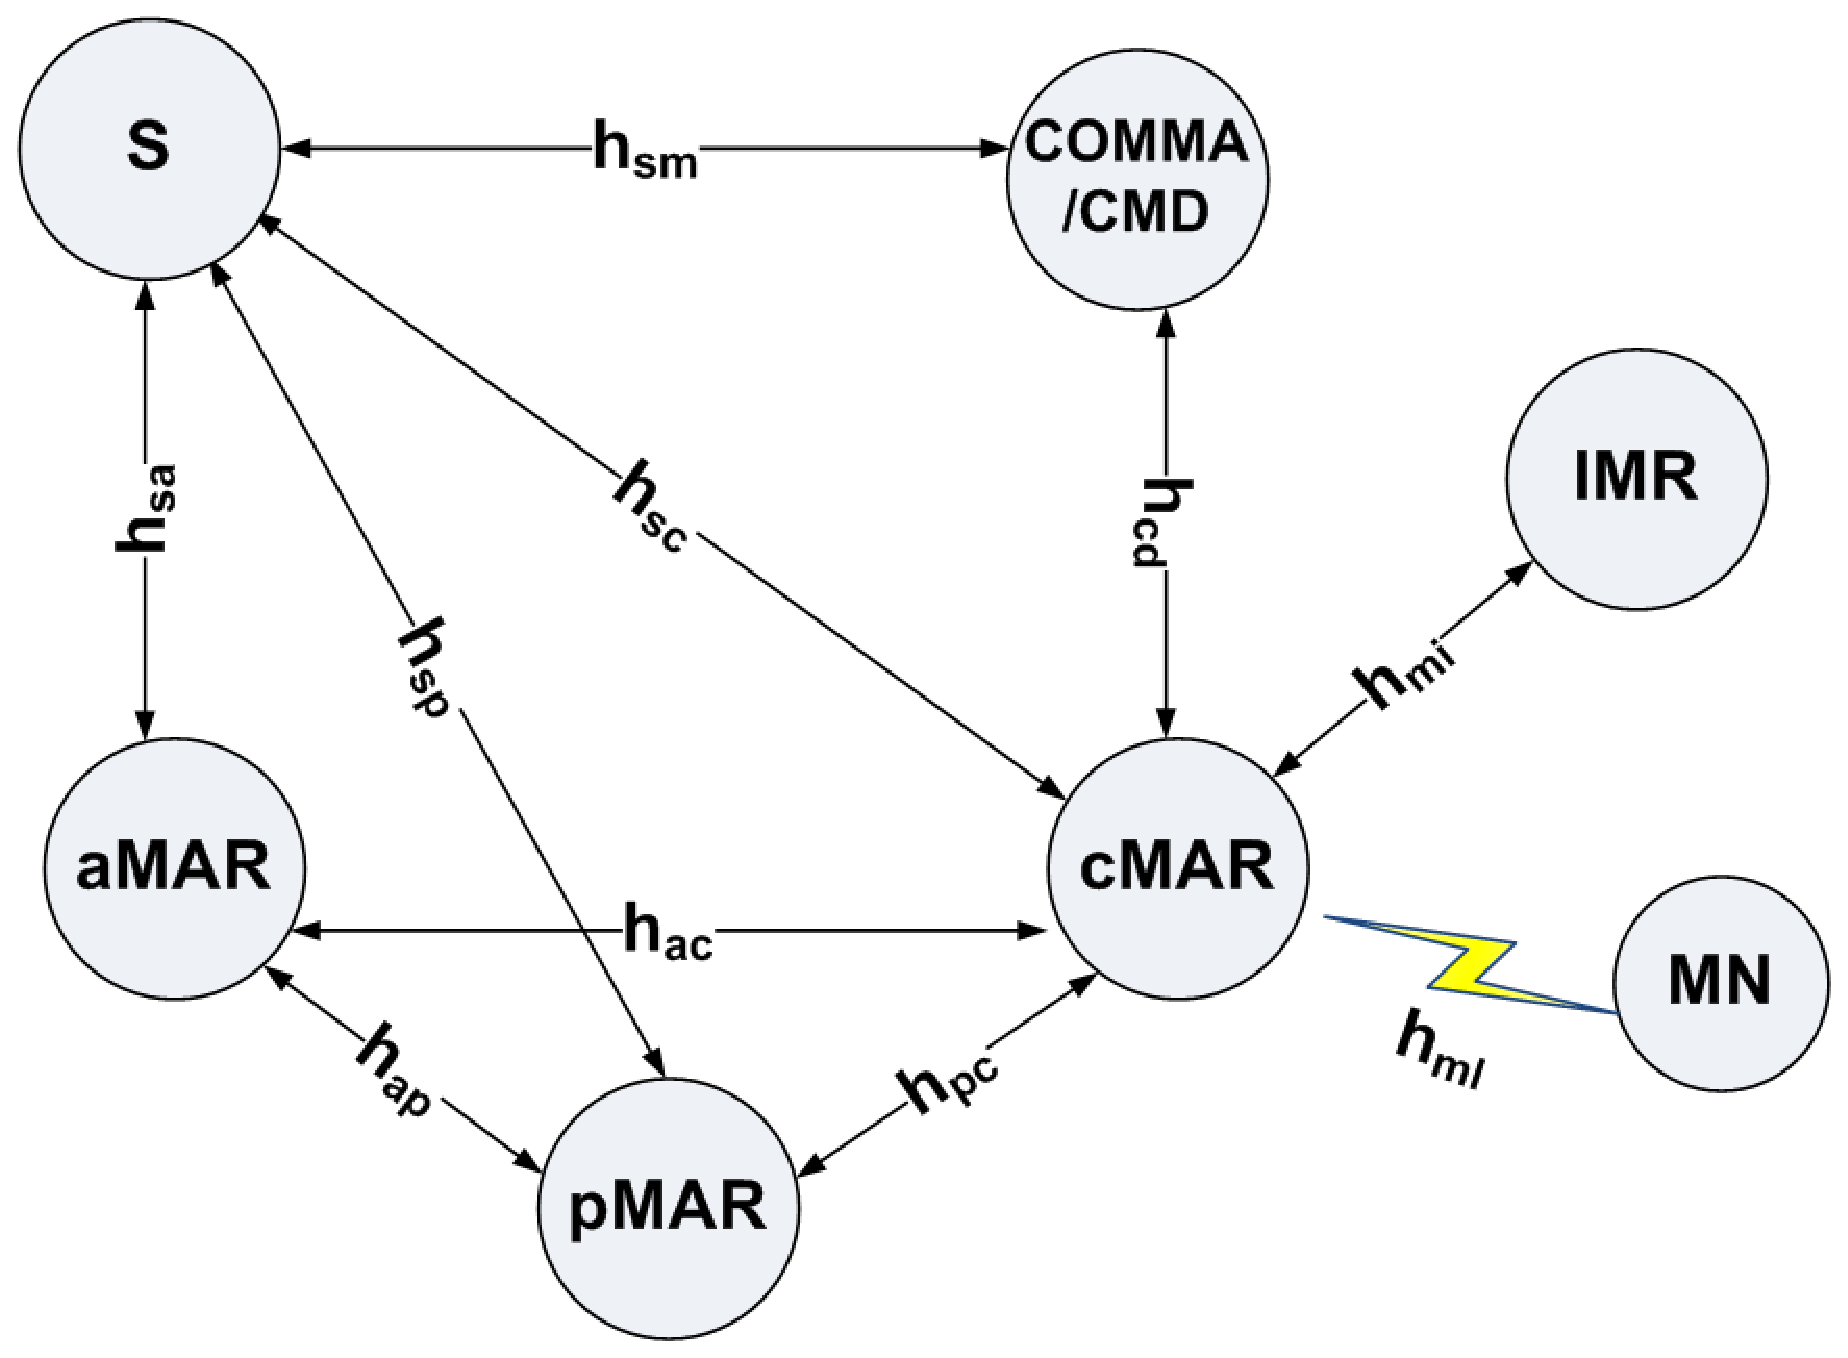
\includegraphics[width=0.55\textwidth]{./Part3/Chapter8/figures/c10_topology_analysis.eps} 
%    \caption{Une topologie de référence du réseau.}
%    \label{fig:c10_topology_analysis}
%  \end{center} 
%\end{figure}
%
%La figure~\ref{fig:c10_topology_analysis} présente une topologie de référence et les distances en saut entre les entités pour l'analyse de performance. A noter que l'intersection MR (IMR) est un router qui possède déjà un état ​​d'acheminement pour le groupe.
%On définit alors l'échelle du réseau $\psi$ qui est le ratio entre le nombre de sauts entre deux MAR adjacents ($h_{mm}$) et le nombre de sauts entre le MAR et le CMD ($h_{cd}$) . \\
%\begin{equation}
%\psi = \frac{h_{mm}}{h_{cd}}.
%\end{equation} 
%En règle générale, le nombre moyen de sauts entre deux MAR adjacents est inférieur à celui entre un MAR et une entité centralisée. Cela signifie que $ \psi \leq 1 $. Dans ce document, nous allons étudier l'impact de l'échelle du réseau sur les métriques de la performance en variant la valeur de $ \psi $ sur un intervalle [0,1].
%
%\paragraph{Les messages liés à l'analyse de performance}
%Dans notre analyse, différents messages sont utilisés. Pour un souci de simplicité, nous supposons qu'il existe un seul flux continu. $L_{RS}$, $L_{RA}$, $L_{PBU}$, $L_{PBA}$, $L_{ePBU}$, $L_{ePBA}$, $L_{M-Req}$, $L_{M-Res}$, $L_{C-Req}$, $L_{C-Res}$, $L_{MLD-R}$, $L_{Join}$, $L_{MP}$, $L_{T}$ est la taille du message Router Solicitation (RS), Router Advertisement (RA), PBU, PBA, PBU étendu, PBA étendu, request de transfert de contexte, réponse de transfert de contexte, demande de configuration de canal, réponse de configuration de canal,  Rapport MLD, PIM Rejoignez, paquet multicast, l'en-tête de tunnel; respectivement.
%
%\paragraph{Le modèle de délai}
%Dans cette thèse, on adopte le modèle de délai de transmission de paquets dans \cite{packet_transmission_delay} dans lequel la transmission de paquets se compose la durée de transmission et le temps de propagation. Ainsi, le délai de transmission d'une liaison filaire peut être calculé comme
%\begin{equation}
%d_{wd}(l,h) = h (\dfrac{l}{BW_{wd}} + D_{wd}),
%\end{equation}
%Où h est la distance en saut entre deux nœuds, l est la taille du paquet, $ BW_{wd} $ est la bande passante de liaison filaire et $ D_{wd} $ est la latence du liaison filaire.
%
%Contrairement à la transmission filaire qui peut être considéré comme fiable, la liaison sans fil n'est pas fiable. Le délai de transmission sans fil est donc calculé comme \cite{packet_transmission_delay} \\
%\begin{equation}
%d_{wl}(l) = \dfrac{1}{1-q} (\dfrac{l}{BW_{wl}} + D_{wl}),
%\end{equation} 
%où q est la probabilité d'échec de liaison sans fil, $ BW_{wl} $ est la bande passante et $ D_{wl} $ est la latence de liaison sans fil.
%
%\paragraph{Le modèle de mobilité}
%Dans ce document, nous considérons le cas où le MN se déplace toujours de MAR à MAR comme s'ils étaient déployés linéaire (l'utilisateur est en train de s'éloigner du premier MAR et jamais s'attache vers un MAR précédemment visité). Il représente le pire des cas. Ainsi, nous avons
%$h_{ac}$ = $h_{ap}$ + $h_{pc}$.
%
%Soit $ N_{mar} $ représente le nombre moyen de MARs impliqués dans le transfert du trafic de données vers / depuis un MN. Dans notre contexte, $ N_{mar} $ est également le nombre de handovers. On obtient donc 
%\begin{equation}
%h_{ac} = N_{mar} h_{mm},
%\end{equation} 
%\begin{equation}
%h_{pc} = h_{mm}.
%\end{equation}
%Dans notre analyse, la valeur basse de $ N_{mar} $ représente le nœud avec la faible mobilité ou le scénario dans lequel le flux est à court durée. La valeur plus élevée de $ N_{mar} $ correspond à la forte mobilité ou le scénario dans lequel le flux est à long terme.
%
%\subsubsection{La modélisation analytique}
%Ce paragraphe développe un modèle d'analyse en ce qui concerne différents paramètres de performance. Dans cette analyse, nous considérons le cas normal et le cas où le proxy MLD supportant la capacité de multiples d'interfaces en amont. Nous soulignons ensuite les impacts et les avantages de l'utilisation de plusieurs interfaces sur ​​ces métriques.
%
%\paragraph{Le temps d'interruption du service}
%Le temps d'interruption ($ SD(.)$) est définie comme une période où un auditeur est incapable de recevoir les paquets multicast. En supposant que le temps associé au traitement des messages dans les entités de réseau (par exemple, le temps de traitement de PBU et de mise à jour de cache dans MAR) est inclus dans la valeur totale de chaque variable. Ensuite, le temps d'interruption est (voir la figure~\ref{fig:c10_HO}). \\
%\small
%\begin{multline}
%SD(.) = T_{L2} + d_{wl}(L_{RS}) + d_{wd}(L_{ePBU},h_{cd}) + d_{wd}(L_{ePBA},h_{cd}) + max \{ d_{wd}(L_{PBA}, h_{ac}) \\+ d_{wd}(L_{PBU}, h_{ac}), d_{wd}(L_{M-Req},h_{pc}) +d_{wd}(L_{M-Res},h_{pc})\} \\ +max \{d_{wl}(L_{MP}), T_{M}{(.)} + d_{wl}(L_{MP})\},
%\label{eq:sd}
%\end{multline}
%\normalsize
%où $ T_{L2} $ est la durée de handover de la couche 2, $T_{M} (.)$ est le temps nécessaire pour le cMAR d'adhérer et obtenir le premier paquet après le handover.
%
%En cas MMA\_cMAR, le cMAR doit obtenir le trafic à partir de l'IMR qui a déjà un état ​​d'acheminement pour ce groupe. Ainsi \\
%\small
%\[ T_{M}(cMAR) = \left\{ 
% \begin{array}{l l}
%   \overline{w}_{mr} \quad \small \text{if } h_{mi} =0,  \\
%   (h_{mi} +1) \overline{w}_{mr}+d_{wd}(L_{MLD-R}) + d_{wd}(L_{MP}) +  d_{wd}(L_{Join},h_{mi}-1) \\+d_{wd}(L_{MP},h_{mi}-1)   \quad \small \text{if }h_{mi} \geq 1. 
% \end{array} \right.\] 
%\normalsize 
%où $ \overline{w}_{m} $ est le délai dans lequel un MR (et un proxy MLD) doit rejoindre un flux multicast à chaque routeur intermédiaire dans l'Internet \cite{MPDSR}.
%
%En cas MMA\_pMAR, le pMAR a eu l'état pour ce flux. Nous avons \\
%\begin{equation}
%T_{M}(pMAR) = 2\overline{w}_{mr} +d_{wd}(L_{MLD-R}+L_{T},h_{pc})+d_{wd}(L_{MP} +L_{T},h_{pc}).
%\end{equation}
%
%En cas MMA\_aMAR, il y a deux possibilités : le cas normal (cas 1, correspond au mode par défaut), et le cas où le proxy MLD supportant plusieurs interfaces « en amont » est déployé dans MARs. Dans ce dernier cas, dans le pire des cas, l'aMAR doit rejoindre le canal multicast, conduisant à un délai supplémentaire. Soit $ p_{a} $ représentent la probabilité que cette situation se produit. En conséquence, $ T_{M}(.) $ est calculé comme \\
%\begin{equation}
%T_{M}(aMAR) =(1-p_{a}) T_{M}(aMAR-c1)  +p_{a} T_{M}(aMAR-wc),
%\end{equation}
%où
%\begin{equation}
%T_{M}(aMAR-c1) =2\overline{w}_{mr} +d_{wd}(L_{MLD-R}+L_{T},h_{ac})+d_{wd}(L_{MP} +L_{T},h_{ac}),
%\end{equation}
%\small
%\[T_{M}(aMAR-wc)  = \left\{ 
% \begin{array}{l l}
%   T_{M}(aMAR-c1)  \quad \small \text{if } h_{mi} =0,  \\
%    T_{M}(aMAR-c1)+ d_{wd}(L_{MLD-R})+ d_{wd}(L_{MP})  + d_{wd}(L_{Join},h_{mi}-1) \\+ (h_{mi}+1)  \overline{w}_{mr} +d_{wd}(L_{MP},h_{mi}-1)  \quad \small \text{if }h_{mi} \geq 1. 
% \end{array} \right.\] 
%\normalsize 
%Il est à noter que $ T_{M} (aMAR-c1) $ représente le temps d'interruption dans le mode par défaut, quand $ T_{M}(aMAR) $ montre l'impact de l'utilisation de proxy avec plusieurs interfaces sur ​​le temps d'interruption. En conséquence, $ SD(aMAR) $ peut être considéré comme un compromis entre l'interruption de service et le problème de la convergence.
%
%Dans le cas MMA\_COMMA, nous avons\\
%\begin{equation}
%T_{M}(COMMA)= 2\overline{w}_{mr}+  d_{wd}(L_{MLD-R}+L_{T}, h_{cd}) + d_{wd}(L_{MP}+L_{T}, h_{cd}).
%\end{equation}
%
%\paragraph{Le délai de bout en bout}
%Le délai de bout en bout ($E2E(.) $) est le délai de transmission de paquets de la source à l'auditeur. Dans le MMA\_cMAR, le cMAR reçoit le trafic multicast directement à partir de l'infrastructure multicast. Par conséquent, le délai de bout-en-bout est donné par \\
%\begin{equation}
%E2E(cMAR) = d_{wd}(L_{MP},h_{sc}) + d_{wl}(L_{MP}).
%\end{equation}
%
%Dans le cas MMA\_aMAR, le paquet multicast est acheminé depuis la source vers le cMAR via l'aMAR, représentant le mode par défaut. Nous avons \\
%\begin{equation}
%E2E(aMAR) = d_{wd}(L_{MP},h_{sa}) + d_{wd}(L_{MP}+L_{T},h_{ac}) + d_{wl}(L_{MP}).
%\end{equation}
%
%En cas MMA\_pMAR, le MAR reçoit toujours le trafic de son pMAR dans le cas normal. Par conséquent, le délai de bout-en-bout est donné comme suit \\
%\begin{equation}
%E2E(pMAR-c1)= d_{wd}(L_{MP},h_{sa}) + d_{wd}(L_{MP} +L_{T},h_{ap}) + d_{wd}(L_{MP} + L_{T},h_{pc})  + d_{wl}(L_{MP}).
%\end{equation}
%
%En cas d'utilisation de proxy avec plusieurs interfaces, nous supposons que $ p_{p} $ est la probabilité que le MAR obtient le trafic multicast d'une interface « en amont ». Ainsi, $ 1-p_{p} $ est la probabilité que le MAR obtient le trafic multicast de son pMAR. Le délai dans le cas MMA\_pMAR est donc donné par
%\begin{multline}
%E2E(pMAR)=   d_{wl}(L_{MP}) + [d_{wd}(L_{MP},h_{sa})+ N_{mar} d_{wd}(L_{MP} +L_{T},h_{mm})] p_{p}^{N_{mar}-1} \\+ \sum_{i=1}^{N_{mar}-1} [d_{wd}(L_{MP},h_{i})+ (N_{mar}-i) d_{wd}(L_{MP} +L_{T},h_{mm})] p_{p}^{N_{mar}-i-1} (1-p_{p}),
%\end{multline}
%où $ h_{i} $ est la distance en saut de la source vers le i$^{ième} $ MAR dans le chemin de déplacement du MN (de l'aMAR au cMAR), par exemple, $ h_{N_{mar}-1} = h_{sp}$.  
%
%Considérant le MMA\_COMMA, le délai de bout en bout est exprimé sous la forme \\
%\begin{equation}
%E2E(COMMA) = d_{wd}(L_{MP},h_{sm})  + d_{wd}(L_{MP}+L_{T},h_{cd}) + d_{wl}(L_{MP}).
%\end{equation}
%
%\paragraph{L'analyse du coût}
%Dans ce paragraphe, le coût de signalisation ($ SC (.) $), le coût de livraison de paquets ($ PC (.) $) et le coût de tunnelisation ($ TC (.) $) sont étudiés. Le coût de signalisation (per handover) est le frais général de signalisation pour soutenir le handover y compris les procédures relatives au multicast. Il peut être calculé comme \\
%\begin{equation}
%SC(.) =SC_{LU} + SC_{M}(.),
%\end{equation}
%où $ SC_{LU}$, $ SC_{M} (.) $ est le coût pour la mise à jour de l'emplacement et les procédures relatives au multicast, respectivement. Le coût de signalisation est calculé comme le produit de la taille du message, la distance et le coût de transmission d'une unité dans une liaison filaire/sans fil ($ \alpha $ pour le liaison filaire et $\beta $ pour la liaison sans fil). $ SC_{LU} $ est donc donné par \ \
%\begin{equation}
%SC_{LU} = \beta (L_{RS} + L_{RA}) + \alpha (L_{ePBU}  h_{cd} + L_{ePBA} h_{cd})  + \alpha (L_{PBU}  h_{ac} + L_{PBA} h_{ac}).
%\end{equation}
%$SC_{M}(.)$ est calculé par\\
%\begin{equation}
%SC_{M}(cMAR) = \alpha  (L_{M-Req}  h_{pc} + L_{M-Res} h_{pc} + L_{MLD-R} + L_{Join} h_{mi}).
%\end{equation}
%\begin{equation}
%SC_{M}(pMAR) = \alpha (L_{M-Req}  h_{pc} + L_{M-Res} h_{pc} + L_{MLD-R} h_{pc}).
%\end{equation}
%\begin{equation}
%SC_{M}(aMAR) =(1-p_{a}) SC_{M}(aMAR-c1)  + p_{a} SC_{M}(aMAR-wc),
%\end{equation}
%où 
%\begin{equation}
%SC_{M}(aMAR-c1) = \alpha (L_{M-Req}  h_{pc} + L_{M-Res} h_{pc} +L_{MLD-R} h_{ac}),
%\end{equation}
%\begin{equation}
%SC_{M}(aMAR-wc) = \alpha (L_{M-Req}  h_{pc} + L_{M-Res} h_{pc}  + L_{MLD-R} h_{ac}+L_{MRD-R} +L_{Join} h_{mi}).
%\end{equation}
%
%\begin{equation}
%SC_{M}(COMMA) = \alpha (L_{M-Req}  h_{pc} + L_{M-Res} h_{pc}  + L_{MLD-R} h_{cd}).
%\end{equation}
%
%Le coût de livraison représente le coût de livraison des paquets multicast pour le MN par unité de temps. Soit $ S_{c} $, $\lambda_{p} $ représentent la durée moyenne des séances au cMAR et le taux d'arrivée des paquets, respectivement. Encore, le coût dans le MMA\_aMAR correspond au mode par défaut. Le coût est exprimé sous la forme \\
%\begin{equation}
%PC(cMAR) = S_{c} \lambda_{p} (\alpha L_{MP} h_{sc}  + \beta L_{MP}).
%\end{equation}
%\begin{equation}
%PC(aMAR) = S_{c} \lambda_{p} [\alpha L_{MP} h_{sa} + \alpha (L_{MP} + L_{T}) h_{ac}  + \beta L_{MP}].
%\end{equation}
%
%En cas MMA\_pMAR, dans le cas normal, le MAR reçoit toujours le trafic multicast de son pMAR. Ainsi, le coût de livraison de paquets est donné comme suit \\
%\begin{equation}
%PC(pMAR-c1)=  S_{c} \lambda_{p} [\alpha  L_{MP} h_{sa} +  \alpha  (L_{MP} + L_{T}) ( h_{ap} + h_{pc}) + \beta L_{MP}].
%\end{equation}
%En utilisant le proxy avec multiples interfaces, le coût de livraison est calculé comme étant
%\begin{multline}
%PC(pMAR)= S_{c} \lambda_{p}  \beta L_{MP} +  S_{c} \lambda_{p} [\alpha L_{MP} h_{sa}+ \alpha N_{mar}  (L_{MP} +L_{T}) h_{mm}] p_{p}^{N_{mar}-1} \\+ S_{c} \lambda_{p} \sum_{i=1}^{N_{mar}-1} [\alpha L_{MP} h_{i}+ \alpha  (N_{mar}-i) (L_{MP} +L_{T}) h_{mm}] p_{p}^{N_{mar}-i-1} (1-p_{p}).
%\end{multline}
%
%En cas MMA\_COMMA, le coût de livraison de paquets est \\
%\begin{equation}
%PC(COMMA) = S_{c} \lambda_{p} [\alpha L_{MP} h_{sm} + \alpha (L_{MP} + L_{T}) h_{cd}  + \beta L_{MP}].
%\end{equation}
%
%En ce qui concerne le coût de tunnelisation, il est défini comme le coût supplémentaire de la tête de tunnel. En MMA\_cMAR, le trafic multicast est reçu directement à partir de l'infrastructure multicast, il n'y a donc pas de coût de tunnelisation. Au contraire, dans les cas MMA\_aMAR, MMA\_pMAR et MMA\_COMMA le trafic est routé via le tunnel aMAR-cMAR, pMAR-cMAR, et cMAR-COMMA, respectivement. A noter que le coût de tunnelisation dans le cas MMA\_aMAR correspond au mode multicast par défaut. Le coût de tunnelisation est donc calculé comme \\
%\begin{equation}
%TC(cMAR) = 0. 
%\end{equation}
%\begin{equation}
%TC(aMAR) = \alpha  S_{c} \lambda_{p} (L_{MP} + L_{T}) h_{ac}. 
%\end{equation}
%\begin{equation}
%TC(pMAR)=  \alpha  S_{c} \lambda_{p} (L_{MP} + L_{T}) h_{mm}  \sum_{i=0}^{N_{mar-1}} (N_{mar}-i)p_{p}^{N_{mar}-i-1} (1-\theta p_{p}).
%\end{equation}
%où  
%\[\theta  = \left\{ 
% \begin{array}{l l}
%   0 \quad \small \text{if } i =0,  \\
%    1  \quad \small \text{if } i \geq 1. 
% \end{array} \right.\] 
%
%\begin{equation}
%TC(COMMA) = \alpha  S_{c} \lambda_{p} (L_{MP} + L_{T}) h_{cd}. 
%\end{equation}
%
%Le coût de signalisation en général, est un facteur important qui influence l'évolutivité du réseau. Cependant, en tant que le plan de données et le plan de contrôle ne sont plus couplés, dans le cas où une grande quantité de trafic est générée dans le réseau, le coût de livraison de paquets et le coût de tunnelisation jouent le rôle plus important.
% 
%\paragraph{La perte de paquets}
%Pendant le handover, les paquets peuvent être perdus. Le nombre de paquets perdus est proportionnel à la durée de l'interruption du service, et le taux d'arrivée des paquets. En conséquence, le nombre de paquets perdus est donné par \\
%\begin{equation}
%\varphi_{p}(.)= \lambda_{p} SD(.).
%\end{equation}
%
%\normalsize
%\subsubsection{Les résultats numériques}
%Ce paragraphe présente les résultats numériques basés sur l'analyse donnée dans le paragraphe précédent. Les valeurs des paramètres par défaut sont présentées dans le tableau \ref{tap:c10_parameters}, dans lequel $L_{PBU}$,  $L_{PBA}$, $L_{ePBU}$, $L_{ePBA}$, $L_{M-Req}$, $L_{M-Res}$, $L_{C-Req}$ et $L_{C-Res}$ sont extraites de l'implémentation réelle de PMIPv6 \cite{oai_pmip} et de fonction de transfert de contexte \cite{d4.4}, tandis que les autres sont de \cite{HO_comparison_Lee, DMM_analysis_Hassan, dsrm, d4.4}. Il est à noter que le $ SD (aMAR-c1) $, $ E2E (aMAR) $, $ SC (aMAR-c1) $, $ PC (aMAR) $ et $ TC (aMAR) $ correspondent au mode par défaut dans notre analyse. \\
%\begin{table}[ht]
%\small
%\caption{Paramètres pour l'analyse de la performance.}
%\label{tap:c10_parameters}
%\centering
%\begin{tabular}{|c |c |c |c |c |c |}%{|l|l|l|l|l|l|}%
%\hline
%\textbf{Paramètre} & \textbf{Valeur} & \textbf{Paramètre} & \textbf{Valeur} & \textbf{Paramètre} & \textbf{Valeur}  \\
%\hline
%$T_{L2}$ & 50ms & $BW_{wd}$  &  100Mbps & $BW_{wl}$  & 11 Mbps\\
%\hline
%  $D_{wd}$& 2ms  & $D_{wl}$ & 10ms & $q$& 0.35  \\
%\hline
%$\overline{w}_{mr}$&  10 ms  & $h_{mm}$ & 3 sauts & $h_{cd}$&  12 sauts  \\
%\hline
%$h_{mi}$& 2 sauts  & $h_{sa}$& 16 sauts  & $h_{sp}$&  16 sauts   \\
%\hline
% $h_{sc}$  & 16 sauts   & $h_{sm}$&  16 sauts &$S_{c} $&  60 s  \\
%%\hline
%%$h_{cm}$& 12 hops  & $R$& 500m  & 1/$\mu_{s}$&  600s  \\
%\hline
%$\lambda_{p}$& 10 paquets/s  & $\alpha$&  1 & $\beta $&  5  \\
%\hline
%$p_{p}$& 0.9  & $p_{a}$&  0.5 & $L_{RS}$ & 52 octets \\
%\hline
% $L_{RA}$& 80  & $L_{PBU}$& 84 & $L_{PBA}$ & 92 octets \\
%\hline
% $L_{ePBU}$&  84 octets  & $L_{ePBA}$, & 128 octets & $L_{M-Req}$ & 86 octets \\
%\hline 
%$L_{M-Res}$ & 104 octets  & $L_{C-Req}$ & 92 octets & $L_{C-Res}$ & 112 octets \\
%\hline
%$L_{MLD-R}$ & 96 octets  &$L_{Join}$ & 110 octets & $L_{MP}$ &  200 octets \\ 
%\hline
% $L_{T}$ & 40 octets  & &  & &   \\ 
%\hline
%\end{tabular}
%\end{table}
%\normalsize
%\paragraph{Le temps d'interruption de service multicast}
%\begin{figure}[!h]
%\centering
%\subfloat[]{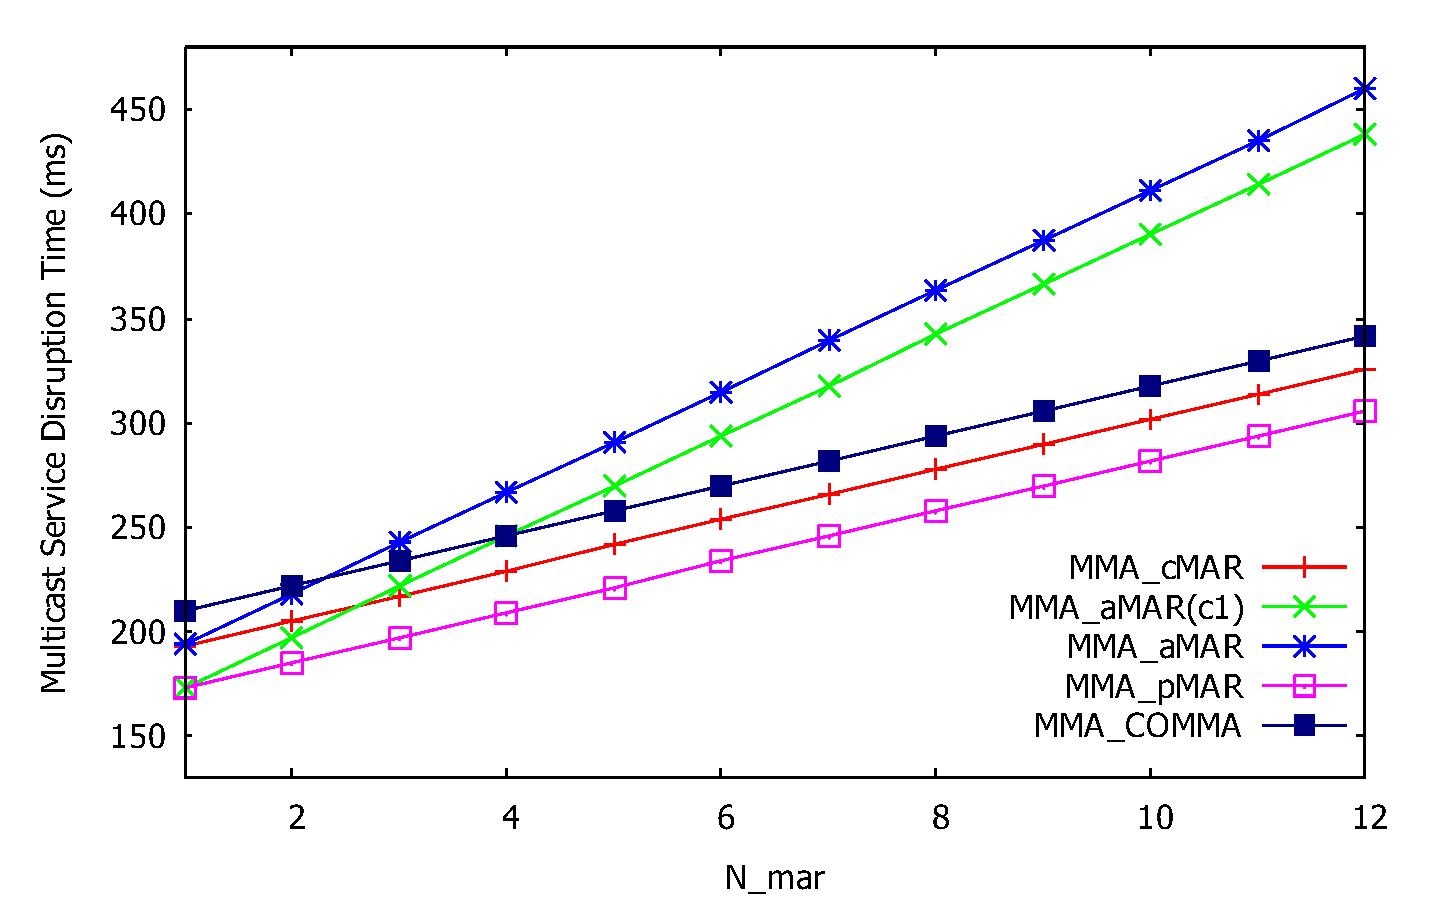
\includegraphics[scale=0.28]{./Part3/Chapter8/figures/c10_sd_n_mar.eps} \label{fig:c10_sd_n_mar}}
%\subfloat[]{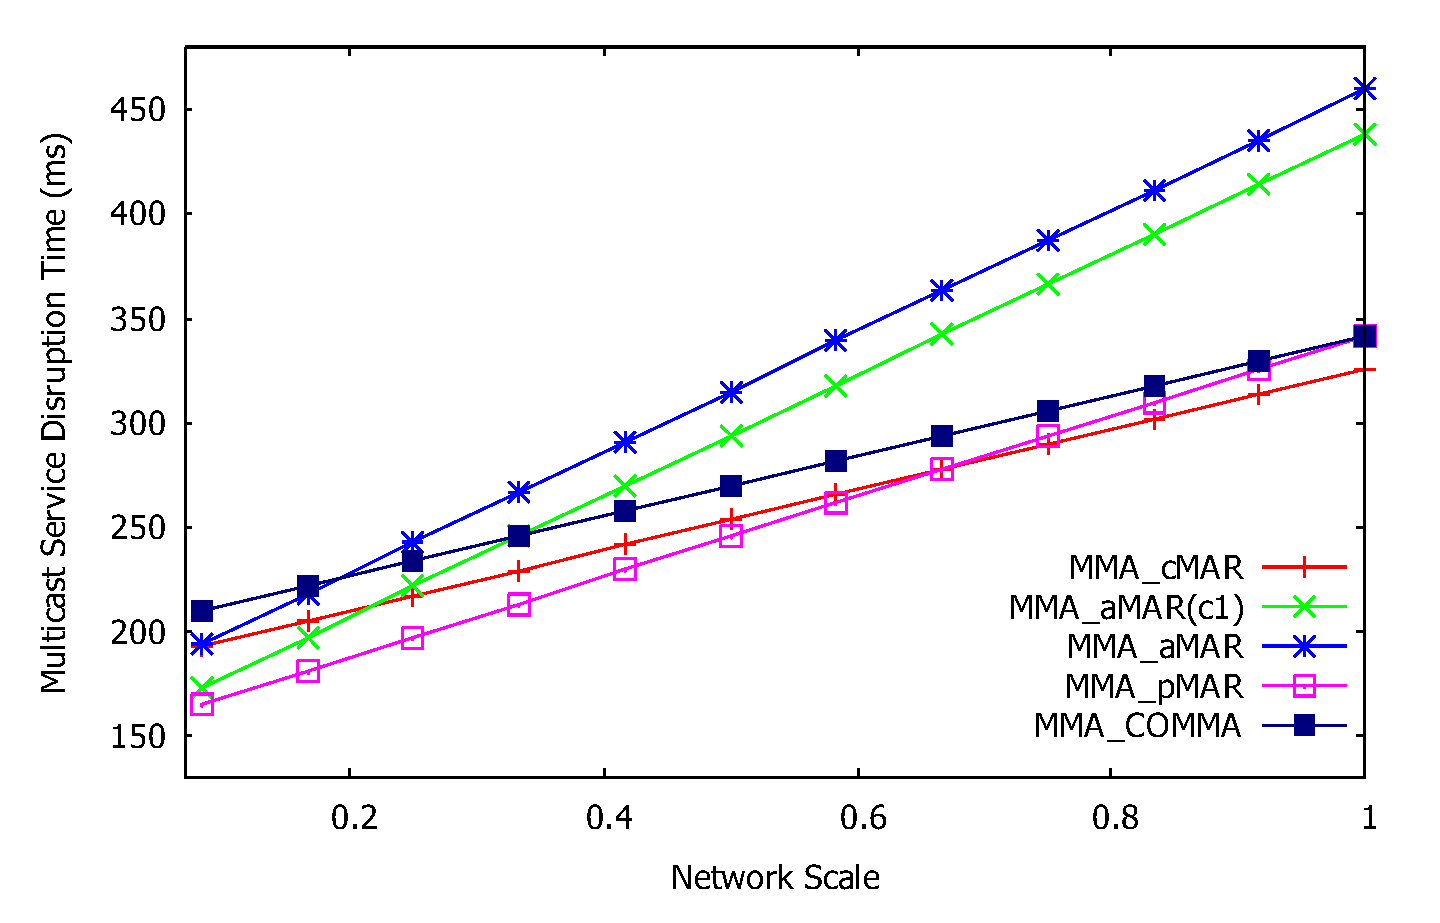
\includegraphics[scale=0.28]{./Part3/Chapter8/figures/c10_scale.eps}\label{fig:c10_scale}}\,
%\subfloat[]{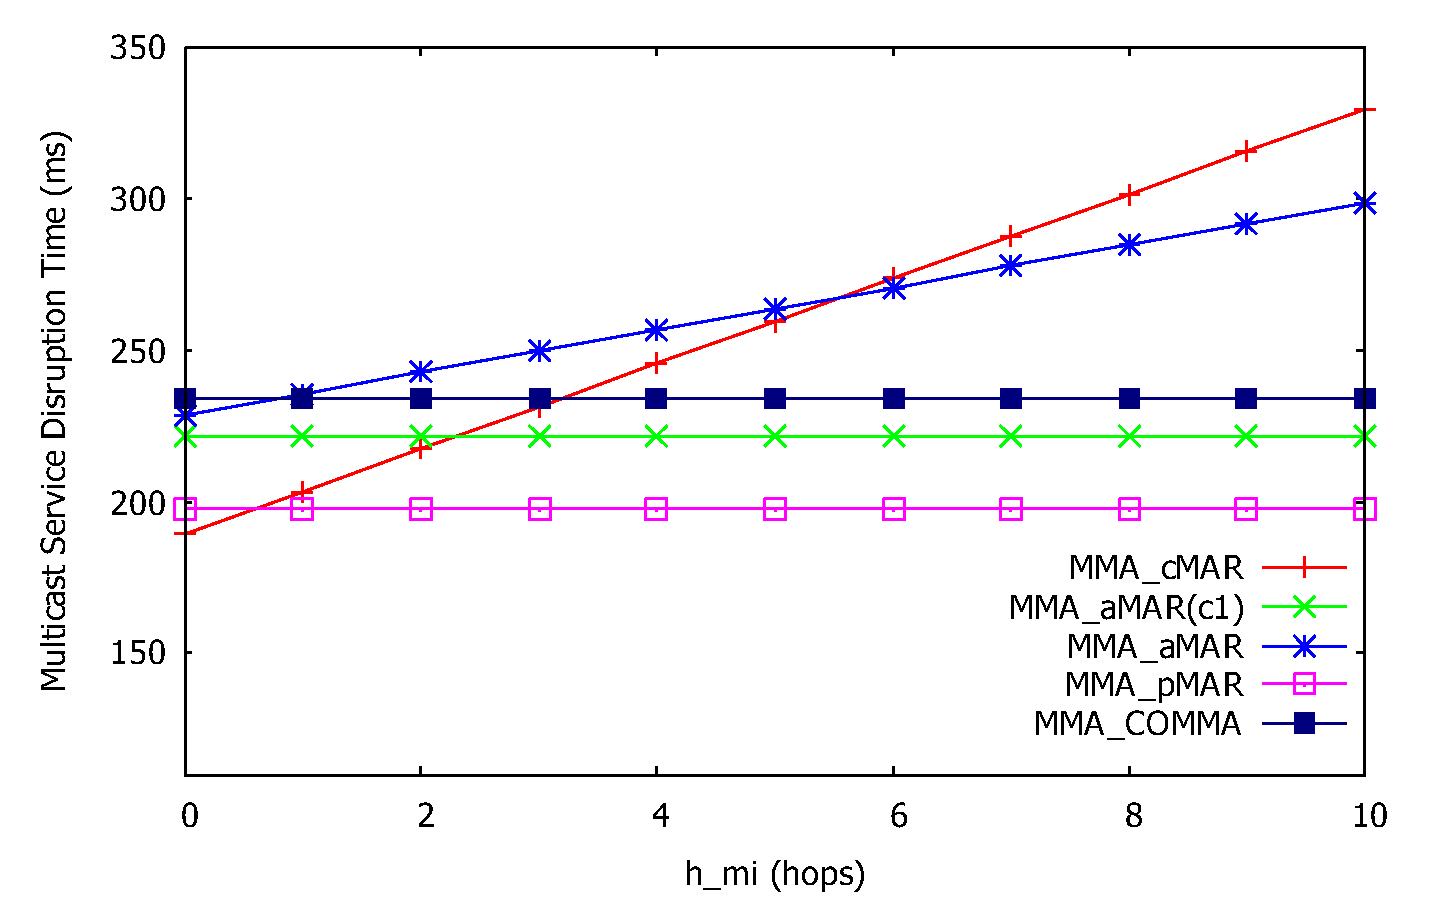
\includegraphics[scale=0.28]{./Part3/Chapter8/figures/c10_h_mi.eps}\label{fig:c10_h_mi}}
%\caption[Le temps d'interruption de service multicast.]{Le temps d'interruption comme une fonction de : (a) $N_{mar}$, (b) $\psi$, (c) $h_{mi}$.} 
%\label{fig:c10_sd}
%\end{figure}
%La figure ~\ref{fig:c10_sd_n_mar} montre le temps d'interruption de service quand $ N_{mar} $ est variée sur une intervalle de 1 à 12. Il apparaît clairement que l'approche MMA\_pMAR donne une meilleure performance que les autres. Lorsque $ N_{mar} $ est faible (moins de 5), toutes les approches satisfont à l'exigence en termes d'interruption pour les services en temps réel (inférieur à 300 ms). Lorsque $ N_{mar} $ est relativement grande, l'interruption de service en cas MMA\_aMAR est significativement augmentée. Nous étudions aussi l'impact de l'échelle du réseau ($\psi $) sur le temps d'interruption. Dans ce cas, $ N_{mar} $ est réglée à une valeur de 3. D'une manière générale, l'impact de $\psi $ est similaire à celui de $ N_{mar} $. Surtout, Fig.~\ref{fig:c10_scale} montre qu'il existe une zone où le MMA\_cMAR surpasse le MMA\_pMAR (lorsque $\psi  \geq 0.62$).\\
%La figure~\ref{fig:c10_h_mi} indique le temps d'interruption lorsque $ h_{mi} $ est variée sur une intervalle de 0 à 10 sauts. Une petite valeur de $ h_{mi} $ indique un scénario de forte densité d'auditeur et une valeur élevée de $ h_{mi} $ représente un scénario de faible densité d'auditeur. Le temps d'interruption dans le MMA\_pMAR est plus faible que dans les autres (sauf si $ h_{mi} = 0 $ indiquant le cas où le trafic multicast est déjà disponible au MR « en amont » du cMAR). Comme la valeur de $ h_ {mi} $ augmente, le temps d'interruption dans le MMA\_pMAR, MMA\_aMAR (c1) et MMA\_COMMA est maintenu constant alors que celui dans les autres cas est considérablement augmenté. Par conséquent, la différence entre les approches est augmentée. En outre, le temps d'interruption dans MMA\_cMAR dépend fortement de la valeur de $ h_{mi} $. En d'autres termes, il ne peut pas être garantie à l'approche MMA\_cMAR. En outre, dans MMA\_aMAR, il augmente de manière significative comparé à celui dans le cas MMA\_aMAR (c1) à la suite de l'utilisation du proxy avec plusieurs interfaces.\\
%\begin{figure}[h!]
%\centering
%\subfloat[]{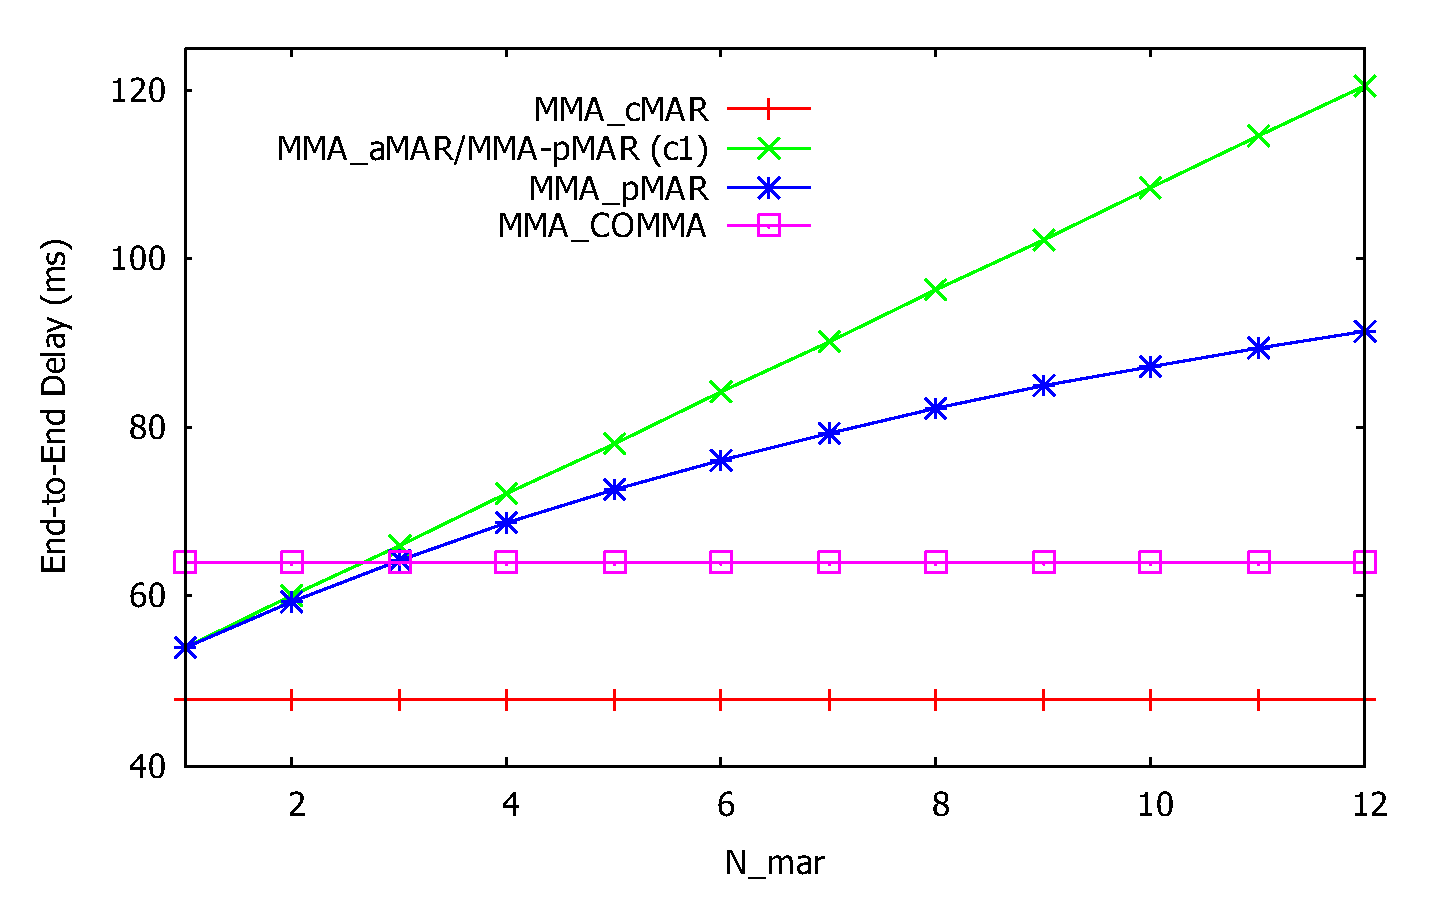
\includegraphics[width=0.50\textwidth]{./Part3/Chapter8/figures/c10_e2e_n_mar.eps} \label{fig:c10_e2e_n_mar}}
%\subfloat[]{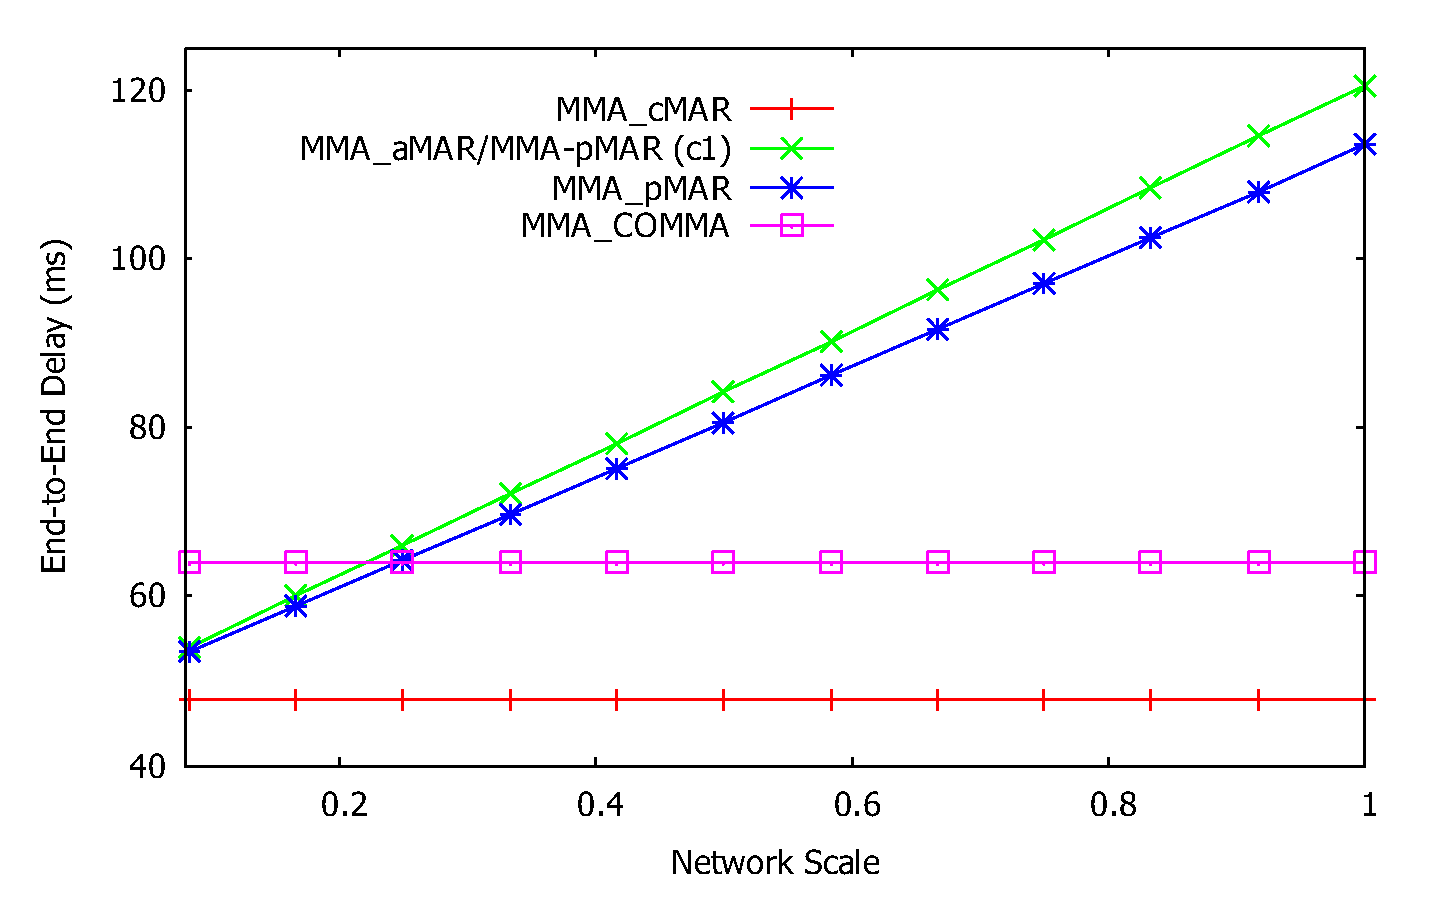
\includegraphics[width=0.50\textwidth]{./Part3/Chapter8/figures/c10_e2e_scale.eps}\label{fig:c10_e2e_scale}}\,
%\subfloat[]{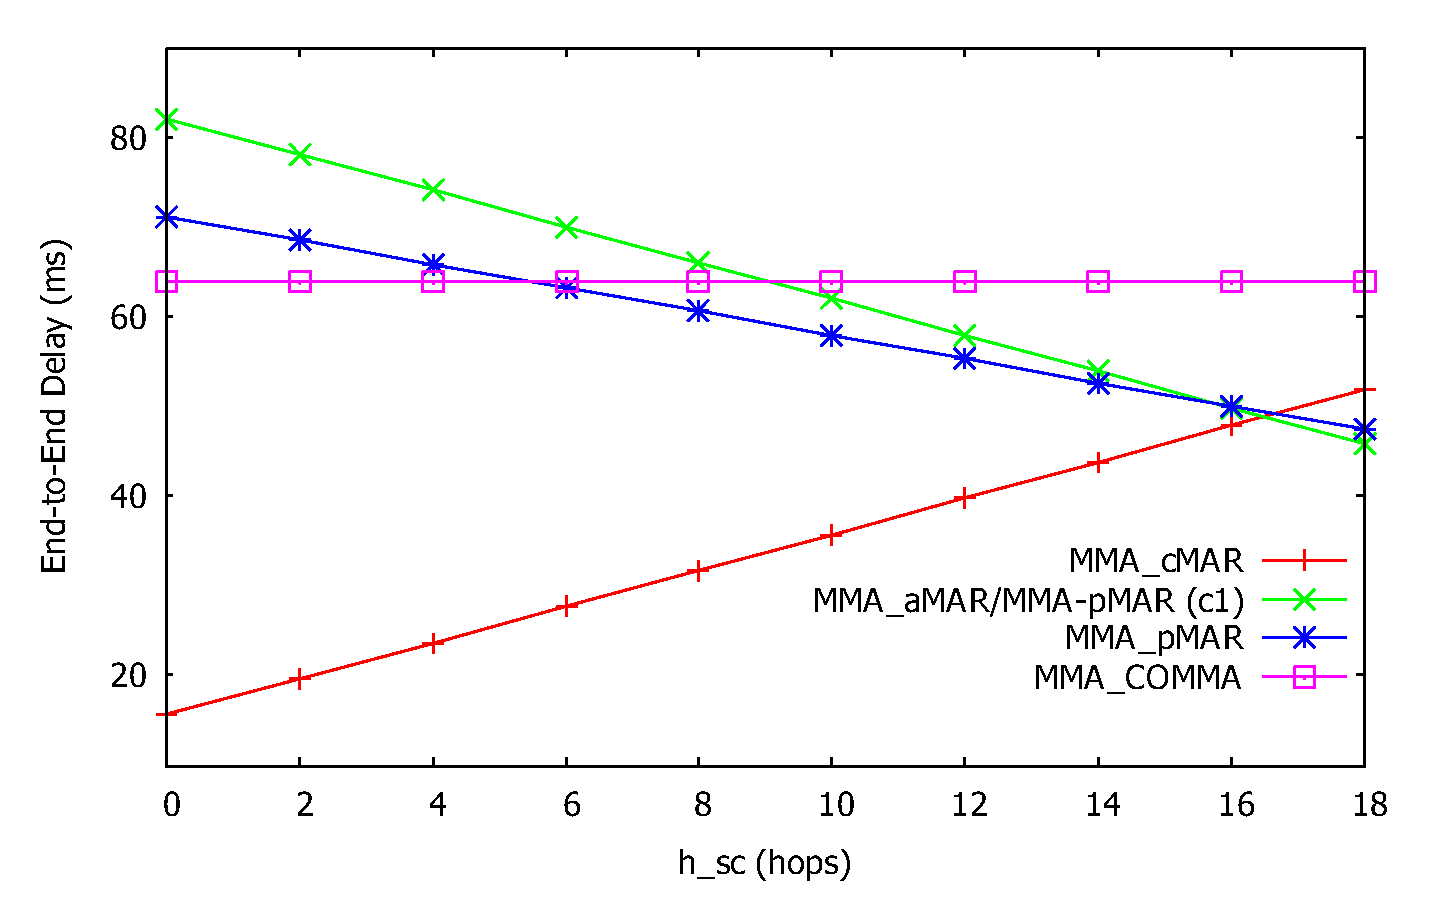
\includegraphics[width=0.50\textwidth]{./Part3/Chapter8/figures/c10_e2e_h_sc.eps}\label{fig:c10_e2e_h_sc}}
%\caption[Le délai de bout en bout.]{Le délai de bout en bout en fonction de : (a) $N_{mar}$, (b) $\psi$, (c) $h_{sc}$.}
%\label{fig:c10_e2e}
%\end{figure}
%En conclusion, l'approche MMA\_pMAR est généralement bien adaptée pour les services sensibles à l'interruption. Ainsi, l'augmentation du temps d'interruption, qui est causée par les multiples interfaces, peut être considérée comme un compromis entre le temps d'interruption et le problème de la convergence.
%\paragraph{Le délai de bout en bout}
%Maintenant, nous étudions l'impact de $ N_{mar} $ sur le délai de bout-en-bout. La figure ~\ref {fig:c10_e2e_n_mar} montre le délai par rapport au nombre de handovers $ N_{mar} $. Comme $ N_{mar} $ augmente ($h_ {ca} $ augmente) le délai en cas MMA\_aMAR et MMA\_pMAR augmente rapidement, tandis que celui dans MMA\_cMAR et MMA\_COMMA est maintenu constant. A noter que le délai dans MMA\_cMAR est maintenu en dessous de la valeur de 50 ms. Cela signifie que MMA\_cMAR satisfait à la exigence stricte en termes de délai de bout-en-bout. Le délai dans MMA\_pMAR (c1) est supérieur à celui dans le MMA\_pMAR à la suite de l'utilisation de multiples interfaces « en amont ». Comme on peut le voir sur la figure~\ref{fig:c10_e2e_scale}. En général, l'échelle du réseau a un impact similaire sur le délai de bout en bout que $ N_{mar} $. La différence majeure est que l'augmentation de la ligne MMA\_pMAR dans la figure~\ref{fig:c10_e2e_scale} est plus rapide que celle dans la figure~\ref{fig:c10_e2e_n_mar}.\\
%Ensuite, $ N_{mar} $ est réglé à une valeur de 6 (correspondant aux flux à moyen / long terme et aux nœuds à moyen / haute mobilité), tandis que la valeur de $ h_ {sc} $ est variée. A ce stade, nous supposons que $h_{sa}$ + $h_{sc} $ est une valeur fixe, par exemple, 18 sauts et $ h_{sp} $ = $ h_{sc} $. Ce scénario est utilisé pour illustrer le cas où la source est très proche de l'aMAR (côté droit de la figure~\ref {fig:c10_e2e_h_sc}) ou  très proche du cMAR (côté gauche de la figure~\ref {fig:c10_e2e_h_sc}). Comme on peut le voir sur la figure~\ref {fig:c10_e2e_h_sc}, même lorsque la source est très proche de l'aMAR, l'approche MMA\_cMAR donne une meilleure performance en termes de délai de bout en bout que les autres. Ainsi, l'impact du tunnel de la mobilité sur le délai est évident. En conclusion, le cMAR est généralement bien adapté pour les flux sensibles aux délais.
%\begin{figure}[h!]
%\centering
%\subfloat[]{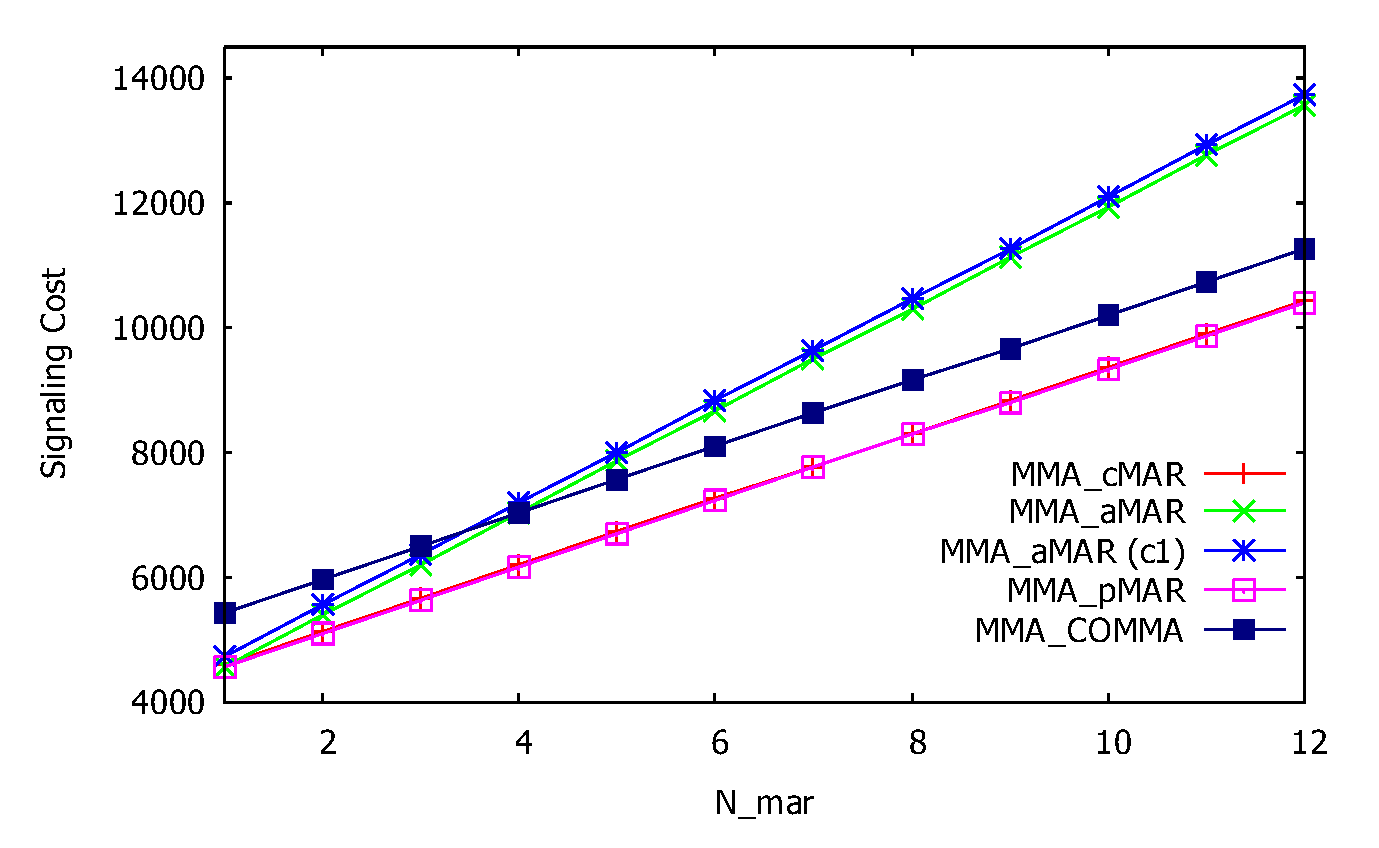
\includegraphics[width=0.50\textwidth]{./Part3/Chapter8/figures/c10_sc_n_mar.eps} \label{fig:c10_sc_n_mar}}
%\subfloat[]{\includegraphics[width=0.50\textwidth]{./Part3/Chapter8/figures/c10_sc_h_mi.eps}\label{fig:c10_sc_h_mi}}
%\caption[Le coût de signalisation.]{Le coût de signalisation comme une fonction de: (a) $N_{mar}$, (b) $h_{mi}$.}
%\label{fig:c10_sc}
%\end{figure}
%\paragraph{Le coût de signalisation}
%La figure~\ref{fig:c10_sc} montre le coût de signalisation en fonction de $ N_{mar} $ et $ h_ {mi} $. En général, le coût de signalisation augmente lorsque $ N_{mar} $ augmente. Sur la figure~\ref{fig:c10_sc_n_mar}, le coût de signalisation dans le cas MMA\_cMAR et MMA\_pMAR est inférieur à celui dans les autres cas. Quand $ N_{mar} $ est assez petite, le coût de signalisation en cas MMA\_COMMA devient plus élevé. Dans le cas contraire, le coût en cas MMA\_aMAR devient plus élevé. Comme on peut le voir sur la figure~\ref{fig:c10_sc_h_mi} (quand $ h_ {mi} $ est variée), le MMA\_pMAR surpasse les autres quand $ h_{mi} $ est supérieur à 2.
%\paragraph{Le coût de livraison de paquets}
%\begin{figure}[h!]
%\centering
%\subfloat[]{\includegraphics[width=0.50\textwidth]{./Part3/Chapter8/figures/c10_pc_n_mar.eps} \label{fig:c10_pc_n_mar}}
%\subfloat[]{\includegraphics[width=0.50\textwidth]{./Part3/Chapter8/figures/c10_pc_h_sc.eps}\label{fig:c10_pc_h_sc}}
%\caption[Le coût de livraison de paquets.]{Le coût de livraison de paquets en termes de: (a) $N_{mar}$, (b) $h_{sc}$.}
%\label{fig:c10_pc}
%\end{figure}
%Similaire au délai de bout en bout, le coût de livraison de paquets (en fonction de $ N_{mar} $) en cas MMA\_cMAR et MMA\_COMMA est maintenu constant tandis que dans le cas MMA\_aMAR et MMA\_pMAR est fortement augmenté. La figure~\ref {fig:c10_pc_h_sc} montre le coût de livraison en fonction de $ h_{sc} $ quand $ h_{sa} + h_{sc} $ est fixé (18 sauts). Il apparaît clairement que le coût dans le cas MMA\_cMAR est nettement inférieur à celui dans les autres, même lorsque la source est très proche de l'aMAR. En outre, nous pouvons observer que ce coût en cas MMA\_pMAR (c1) est supérieur à celui de MMA\_pMAR en raison de multiples interfaces.
%\begin{figure}[h!]
% 	\begin{center} 
%		\includegraphics[width=0.50\textwidth]{./Part3/Chapter8/figures/c10_tc_n_mar.eps}
%		\caption[Le coût de tunnelisation.]{Le coût de tunnelisation comme une fonction de $N_{mar}$.}
%		\label{fig:c10_tc_n_mar}
%	\end{center}
%\end{figure}
%\paragraph{Le coût de tunnelisation}
%En ce qui concerne le coût de tunnelisation, la figure~\ref {fig:c10_tc_n_mar} montre le coût de tunnelisation en fonction de $ N_{mar} $. Le MMA\_cMAR n'introduit pas des surcharges de tunnel, alors que le coût de tunnelisation dans le MMA\_COMMA est fixé. D'autre part, il est significativement augmenté quand $ N_{mar} $ augmente en cas MMA\_aMAR et MMA\_pMAR. Encore une fois, en appliquant les multiples interfaces, le coût de tunnelisation en cas MMA\_pMAR augmente légèrement.
%
%\subsubsection{Conclusion de la partie d'analyse quantitative}
%De l'analyse de la performance et des résultats numériques, nous concluons qu'aucune des approches est toujours meilleure que les autres. Par exemple, le MMA\_pMAR est généralement un bon choix lorsqu'on considère l'interruption de service. Le MMA\_cMAR, en revanche, est un choix préféré en ce qui concerne le délai de bout en bout. Les autres approches peuvent être les plus appropriées, cependant, dans une situation spécifique. L'analyse de performance donne aussi une idée de l'utilisation d'un MMA commun (COMMA) qui sert comme un point d'ancrage seule ​​pour le service multicast pour tous les nœuds dans le domaine, donc reflétant le déploiement PMIPv6. Bien que cette approche présente une performance acceptable, par exemple, quand $ N_{mar} $ et $ \psi $ sont petites, COMMA pose un goulot d'étranglement et un point de panne unique. COMMA n'est pas non plus un bon choix quand un contenu local est disponible. Par conséquent, la comparaison entre le MMA\_COMMA et le mode par défaut donne l'idée de la performance de DMM en ce qui concerne PMIPv6 concernant le service multicast.
%
%Essentiellement, la performance des méthodes dépend de différents facteurs tels que le nombre de handovers ($ N_{mar} $, qui peut être considérée comme une fonction de la vitesse et du rayon de sous-réseau), l'échelle de réseau ($ \psi $), la position de la source ($h_{sc} $, $ h_{sa} $) et la densité de l'auditeur ($ h_{mi} $). Ce sont les raisons pour lesquelles un MMA fixe n'est pas une bonne stratégie. En outre, les utilisateurs mobiles quotidiens consacrent jusqu'à 62 \% de leur temps à la maison et au travail (en général, l'emplacement typique) \cite{cisco_connected_lives}. Ainsi, dans certains cas, l'emplacement typique serait également un bon candidat. Même les ancres de mobilité sont distribuées, certaines d'entre elles sont surchargées plus que les autres \cite{anchor_selection}. En conséquence, un support par flux de multicast doit être fourni.
%
%\subsection{La sélection dynamique de l'ancre multicast} \label{c10:dmma}
%Dans ce paragraphe, un mécanisme de sélection dynamique de l'ancre de mobilité multicast sera introduit. Sur la base des contextes collectés, le MMA sera sélectionné de façon dynamique afin de répondre à un ensemble des exigences. D'un point de vue du service, il contribue à satisfaire les exigences en termes de l'interruption de service et le délai, en particulier lorsqu'on considère des services en temps réel. Il fournit également un mécanisme permettant de mieux répartir la charge entre MARs. D'autres problèmes telles que la duplication de paquets et le laisser la latence (perte de ressources) peuvent être réduits. La sélection de MMA prend en compte non seulement le contexte de service multicast, mais aussi le contexte de la mobilité du nœud et le contexte de réseau, ainsi permettant une support multicast par flux. En d'autres termes, chaque flux multicast peut être traité différemment selon ​​differents contextes. La sélection de MMA peut être fait dynamiquement quand un flux est initié ou lorsque l'auditeur effectue un handover grâce au proxy MLD supportant plusieurs interfaces en amont.
%
%Pour sélectionner dynamiquement le MMA approprié, des contextes différents doivent être pris en compte comme le contexte de service multicast, le contexte de la mobilité du MN, et le contexte de réseau. Chaque contexte peut être affecté à un numéro de priorité. Par exemple, une valeur plus faible indique que le contexte est plus important. A ce stade, similaire au mode par défaut, quand un auditeur initie un flux multicast, le cMAR servira comme le MMA pour ce flux (le trafic multicast sera reçu directement à partir de l'infrastructure multicast). Cela signifie que la sélection MMA dans la phase initiale sera laissée pour les travaux au futur. Pour un flux de handover, le trafic multicast peut être reçu de l'aMAR, le pMAR, le cMAR, ou même un MAR dans lequel le canal multicast est déjà disponible, ou un MAR moins chargé afin de répondre à un ensemble des exigences. 
%
%Notre solution n'est pas seulement pour les problèmes de l'interruption de service et de délai de bout en bout, mais aussi pour autres problèmes liées au service multicast. Ainsi, elle peut offrir des avantages tels que :
%
%\begin{itemize}
%\item \textit{Une solution complète} pour la plupart des problèmes de l'auditeur liées à la mobilité (y compris l'interruption de service, le problème de convergence, le laisser de latence, le gaspillage des ressources, le routage sous-optimal et la perte de paquets);
%\item \textit{La route optimale} : Les flux multicast seront acheminés dans un mieux chemin, car ils ne passent pas toujours par leur ancre de mobilité.
%\item \textit{Evitant du problème de convergence du tunnel} : Cette solution peut résoudre complètement le problème de la convergence;
%\item \textit{L'utilisation dynamique de tunnel de mobilité} : L'utilisation de tunnel de la mobilité pour les sessions multicast en cours est activée dans les cas appropriés, par exemple, pour un contenu à distant, ou un canal avec des exigences de délai très strict;
%\item \textit{Gestion efficace du tunnel} : Dans un environnement DMM, il est impossible d'effectuer une pré-établir tous les tunnels entre MARs puisque le nombre de MARs est censé être grand. En permettant au proxy MLD avec multiples interfaces en amont, il peut causer la gestion complexe de tunnel (par exemple, l'entretien et la vie du tunnel). Ainsi, la solution proposée, qui est basée sur le module de gestion de la mobilité multicast, peut aider à résoudre ce problème;
%\item \textit{Répartition de la charge de flux multicast} : Puisque la sélection MMA prend la charge actuelle du MAR en compte, elle permet de meilleur répartir la charge de trafic multicast entre MARs.
%\item \textit{La gestion centralisée des canaux multicast} : L'entité centrale (Multicast Control Entity, ou MCE) recueille et gère les contextes considérés (par exemple, les canaux multicast et leur portée (locale ou distante)), améliorant le contrôle des fournisseurs de réseau;
%\item \textit{Possibilité d'être appliquée à la mobilité de la source multicast};
%\item \textit{Compatibilité avec la mobilité unicast}.
%\end{itemize}
%
%\subsubsection{Les contextes considérés}
%\paragraph{Le contexte du service multicast}
%Lorsque les services sont sensibles à l'interruption ou à la perte de paquets, le temps d'interruption de service doit être minimisé. Par exemple, il devrait être inférieur à 300ms pour un service en temps réel, tandis que 500 ms pour un service normal \cite{interruption_requirements}. Pour le service sensible au délai de bout en bout, un long tunnel de mobilité ce qui peut entraîner un haut retard, doit être évité. La recommandation UIT-T G.114 \cite{itu-t} suggère que si le temps de transmission unidirectionnelle de connexion peut être maintenu en dessous de 150 ms, la plupart des applications connaîtront une interactivité transparente. En outre, les flux à longue durée peuvent effectuer de nombreuses handovers tandis que les flux à courte durée semblent être lancé et terminé au même MAR sans effectuer aucun handover.
%\paragraph{Le contexte du nœud mobile}
%Un nœud mobile à haute mobilité effectue souvent des handovers. Si le trafic multicast est toujours acheminé par aMAR, le temps de séjour plus long, le plus grave de l'impact sera. En outre, le nombre de points d'ancrage et de tunnels peut être augmenté. Au contraire, pour le nœud de faible mobilité, le MN devrait rester à un ou plusieurs MARs la plupart du temps.
%\paragraph{Le contexte du réseau}
%La sélection MMA peut également être basée sur plusieurs contextes de réseau tels que la charge actuelle de MAR, la proximité géographique du MAR au MN ainsi que la politique de canal multicast. Par exemple, lorsque la charge de MAR est élevée, il peut entraîner de retard et de perte de paquets si ce MAR est sélectionné comme un point d'ancrage multicast. Dans ce cas, le moins chargé MAR (entre MARs qu'ont l'état de transmission multicast pour ce canal) peut être un candidat potentiel. La raison est  que si le canal est déjà disponible au MAR sélectionné, le temps d'interruption peut être réduit au minimum (pas besoin de temps pour rejoindre le canal multicast). En outre, avec une augmentation négligeable de la charge, ce MAR peut transférer le trafic vers le cMAR \cite{developing_ip_multicast}.
%
%\subsubsection{La description de l'architecture de la solution proposée}
%Afin de collecter et gérer les contextes considérés, une entité de réseau, appelé MCE est introduite. Le MAR met régulièrement à jour le contexte de MN et la charge actuelle de MAR au MCE en utilisant une extension de PBU / PBA (ou une extension de messages Heartbeat \cite{heartbeat}). Le MCE gère également tous les canaux multicast dans le domaine. Le contexte de service peut être définie basé sur la classe de QoS.
%
%Résidant dans le MAR, le module de gestion de la mobilité (MUMO) prend la responsabilité de toutes les actions liées à la mobilité multicast. La structure de ce module est illustrée dans la figure~\ref{fig:multicast_module} et brièvement décrite comme suit :
%\begin{figure}[t!]
% 	\begin{center} 
%		\includegraphics[width=0.80\textwidth]{./Part3/Chapter8/figures/c10_mume.eps}
%		\caption{Le module de gestion de la mobilité multicast (MUMO) à MAR.}
%		\label{fig:multicast_module}
%	\end{center}
%\end{figure}
%
%\setlength \abovedisplayskip{-1pt}
%\vspace{-0.1in}
%\begin{itemize}
%\itemsep 0.07em
%\item La fonction de gestion de groupe multicast (MGMF) réfère aux opérations de gestion de groupe et de stockage de l'information, qui est basée sur le proxy MLD avec plusieurs interfaces en amont\footnote{Ce module peut également être invoqué la fonction de routeur multicast par exemple, MRDv6.}. Ce module prend également en charge la fonction explicite de suivi afin de maintenir un état ​​du groupe de multicast par le client \cite{explicit_tracking}. Elle se fait sur ​​la base de Multicast Mobility Database (MMD), qui stocke les entrées avec les informations suivantes : i) l'identification de MN (MN\_ID); l'adresse de MN; et les abonnements des MNs. En outre, il maintient une structure de compteur pour le nombre d'auditeurs par canal multicast, ce qui permet d'identifier si un nœud est le dernier abonné du groupe.
%\item La fonction de gestion de contexte (CMF) communique avec le MCE pour récupérer les informations de configuration de canaux, y compris l'adresse de MMA correspondant, et le type de MMA (le précédent, l'ancrage, et le MAR courant ou autre). Basé sur cette information, le proxy MLD configure ses interfaces en amont vers les MARs correspondants.
%\item La fonction de transfert de contexte multicast (MCTF) est responsable d'échanger des informations d'abonnement multicast de MN entre MARs. Alors que le nouveau MAR peut rejoindre le flux courant à l'avance pour minimiser le temps d'interruption.
%\item La fonction de gestion de mobilité (MMF) ressemble à la pile de protocole de mobilité. Elle est responsable de l'attribution et le maintien de la connectivité IP d'un MN exécutant un handover à l'intérieur du domaine DMM. En d'autres termes, il est responsable de toutes les actions liées à la gestion de mobilité.
%\end{itemize}
%\begin{figure}[tb!] 
%  \begin{center} 
%    \includegraphics[width=0.85\textwidth]{./Part3/Chapter8/figures/c10_service_disruption_CXT_MMA.eps} 
%    \caption{La signalisation liée au service multicast avec la fonction de transfert de contexte multicast.}
%    \label{fig:c10_handover_signaling}
%  \end{center} 
%\end{figure}
%
%\subsubsection{Les opérations de la solution proposée}
%Les opérations de la solution sont brièvement présentées comme suit. Une fois que le MN entre dans un domaine de DMM (attache à MAR1), un préfixe est attribué à lui (dire Pref1). Le MAR1 envoie alors un message PBU y compris l'identification du MN (MN\_ID) et le Pref1 au CMD pour enregistrer ce MN. Après avoir reçu le PBU, le CMD crée une BCE qui se compose du MN\_ID, le Pref1, et l'adresse de MAR1 (comme aMAR) pour ce MN. En réponse, le message PBA est envoyé de CMD à MAR1 pour informer que l'emplacement de MN est mis à jour. Le MAR1 envoie un message RA y compris le Pref1 au MN. Le MN, après avoir configuré son adresse IPv6, peut adhérer à un flux multicast via le MAR courant.
%
%En cas de handover (voir figure ~\ref{fig:c10_handover_signaling}), le cMAR alloue un nouveau préfixe pour ce MN (appelé Pref2). Le cMAR envoie alors un PBU au CMD pour le nouveau enregistrement de préfixe. Ce message comprend le MN\_ID, et le Pref2. En regardant le tableau BCE, le CMD met à jour l'entrée correspondante au MN\_ID à l'emplacement actuel du MN. Le CMD répond alors par un message PBA, y compris la liste des adresses des points d'ancrage, les préfixes correspondants, et l'adresse du MAR précédent. À la réception de ce message, le cMAR échange les messages PBU/PBA avec MARs d'ancrage pour mettre à jour l'emplacement actuel du MN. Ainsi, le tunnel bidirectionnel est établi entre le cMAR et l'aMAR, si nécessaire. Le cMAR envoie alors un message RA, y compris le nouveau préfixe alloué au MN. Le MN peut donc configurer son adresse IPv6 et commencer une nouvelle communication avec le CN. En parallèle, les messages de transfert de contexte multicast sont échangés entre le cMAR et le pMAR permettant le cMAR d'obtenir les flux multicast en cours. Basé sur ces informations, le cMAR contacts avec le MCE pour obtenir les configurations de canaux qui composent les informations suivantes (par canal) : S, G, l'adresse de MMA, et un champ indiquant le rôle de MMA. Les messages PBU / PBA peuvent être étendus à transmettre la configuration de canal. Le cMAR configure une interface en amont vers le MMA, et envoie un rapport MLD au MMA pour rejoindre le canal multicast en cours. Après avoir rejoint l'arbre de transmission multicast (si nécessaire), le MMA transmet les paquets multicast au cMAR, et ils ont finalement atteint le MN. Si le cMAR ne reçoit pas le trafic multicast du pMAR, il demandera le pMAR pour arrêter la transmission du flux. Merci à la fonction explicite de suivi, le pMAR s'arrête la transmission du flux si le MN est le dernier membre de ce flux. Ainsi, il réduit le temps de latence et le gaspillage des ressources.
%
%\subsubsection{L'implémentation de la solution proposée}
%Une première version du DMMA était disponible grâce au projet Medieval \cite{d4.4, d6.4, ICC_Sergio}. Dans ce mode de réalisation, le module CMF exécute de façon simple : lorsque le MN agit comme un auditeur, le cMAR joue toujours le rôle du MMA. Au contraire, l'aMARs agit comme le MMA lorsque le MN joue le rôle d'une source. Cependant, les procédures pour l'acquisition des contextes considérés sont encore en cours de développement. Le module MMF est aussi en cours de développement basé sur la mise en œuvre de l'OAI PMIPv6. Les autres modules comme le MGMF et le MCTF sont déjà disponibles. Dans la prochaine étape, la mise en œuvre complète du module CMF sera déployée. Des expériences seront ensuite effectuées basé sur un banc d'essai proche d’un réseau réel.
%
%\vspace{-0.1in}
%\section{Conclusion et Perspectives}
%Le volume de données dans les réseaux mobiles est en plein essor principalement dû au succès des smartphones et des tablettes. Basé sur le fait que le trafic de l'Internet mobile sera dominé par la vidéo, l'évolutivité et l'efficacité de la bande passante de routage multicast permettent le multicast IP jouera un rôle plus important. Cependant, quand considérant le multicast IP dans un environnement mobile sans fil, il soulève plusieurs problèmes telles que l'interruptions de service, le délai de bout-en-bout, la duplication de paquets, le routage non-optimal et le gaspillage de ressources.
%
%Pour résoudre ces problèmes, cette thèse propose des solutions dans les environnements PMIPv6 et DMM. Grâce à cette thèse, les objectifs suivants sont atteints :
%\setlength \abovedisplayskip{-1pt}
%\vspace{-0.1in}
%\begin{itemize}
%\itemsep 0.07em
%\item \textit{Identifier les enjeux et les défis de la mobilité d'un nœud multicast et des métriques pour évaluer le mécanisme pour la mobilité d'un nœud multicast}
%\item \textit{Proposer une méthode expérimentale pour atteindre les résultats réalistes à faible coût} : La méthode expérimentale est proposé comme une combinaison des techniques de la virtualisation et de la simulation. Un banc d'essai PMIPv6 a été donc mis en œuvre.
%\item \textit{Présenter une méthode efficace pour optimiser la continuité de service en PMIPv6 et déployer un banc d'essai proche d’un réseau réel pour la mobilité d'un nœud multicast} : La solution proposée est basée sur le transfert de contexte multicast et la fonction de suivi explicite permettant au nouveau MAG pour obtenir les informations d'abonnement de MN à l'avance, ce qui réduit l'interruption de service.
%\item \textit{Proposer un mécanisme d'équilibrage de charge des flux multicast dans PMIPv6} : La solution proposée permet de mieux répartir la charge entre LMAs à améliorer l'évolutivité et la fiabilité du système.
%\item \textit{Introduire une solution pour le handover d'un nœud avec multiples interfaces dans des réseaux hétérogènes} : L'interface logique est utilisé en tant que la couche abstraite pour masquer le changement de l'interface physique de la pile IP. Merci à ce mécanisme, le MN n'est pas conscient de la mobilité du point de vue du service multicast. 
%\item \textit{Présenter un support à la mobilité inter-domaine pour les réseaux PMIPv6 et un support de base pour la mobilité de l'auditeur dans un environnement inter-domaine.}
%\item \textit{Proposer un mécanisme de sélection dynamique de l'ancre de mobilité multicast (DMMA) dans l'environnement  DMM}: Le DMMA non seulement supporte les services pour satisfaire l'exigence stricte en termes d'interruption et de délai de bout en bout, mais offre également des avantages tels que l'évitement du problème de la convergence, la gestion efficace du tunnel, le routage optimal, la réduction du gaspillage de ressources et la répartition de la charge.
%\end{itemize}
%
%\paragraph{Les bénéficie des solutions proposées}
%Une partie du mécanisme DMMA a été mis en œuvre dans le projet MÉDIÉVAL. Ce projet vise à fournir une architecture pour améliorer l'Internet mobile actuel et fournir des applications vidéo mobiles de manière plus efficace. Une solution multi-couche a été développée dans laquelle deux services typiques liés au multicast sont considérés comme le Mobile TV et le PBS. En ce qui concerne le support de la mobilité de nœud multicast, une solution à la fois pour l'auditeur et la source dans DMM a été fournie. Dans le cadre de la solution globale, le module de mobilité de multicast qui gère le soutien à la mobilité IP pour les flux multicast a été mis en œuvre. En plus d'informations, le transfert de contexte de multicast et la fonction explicite de suivi sont utilisés pour accélérer le processus d'acquisition de souscription du MN à réduire le temps d'interruption. Pour l'auditeur, le paquet multicast est toujours reçu directement de l'infrastructure multicast au MAR courant. Pour la source, le paquet multicast est acheminé à partir du MAR courant à celui d'ancrage par le tunnel de mobilité. 
%
%Dans le projet VELCRI, la solution pour un handover  sur ​​des réseaux hétérogènes est une partie du système de communication (y compris la communication véhicules-au-Grid et la communication Grid-aux-véhicules) pour fournir le service de charge pour le véhicule électrique. Le système de communication permet à l'EV à toujours être relié au Smart Grid en utilisant différentes technologies dans les différentes phases telles que LTE tout en conduisant, WLAN en approchant une station de recharge, et PLC tout en étant amarré à une station de recharge.\\ 
%Dans le projet SYSTUF, le DMMA sera utilisé pour fournir le service multicast pour les utilisateurs sur les transports publics, par exemple dans le tram et le métro. Dans plus de détails, le but du projet est de définir et de mettre en œuvre de nouveaux services à haut débit et un système de communication entre le sol et les véhicules en mouvement pour améliorer la qualité des transports urbains. Le DMMA sera étudié dans un scénario de forte mobilité.
%\paragraph{Perspectives}
%Avec la volonté de soutenir les services multicast IP dans un environnement mobile sans fil, cette thèse propose des solutions pour les problèmes liés à la mobilité d'un nœud multicast. Toutefois, puisqu'il y a plusieurs sujets définis, plusieurs aspects ne peuvent pas être analysés dans les détails, ce qui peuvent potentiellement être améliorés. Par exemple, alors que l'objectif de cette thèse a été jusqu'ici sur la mobilité de l'auditeur de multicast, la même idée peut être appliquée à la mobilité de la source. 
%
%Un autre sujet, qui serait considéré, est la mobilité du nœud. Autres modèles de mobilité seraient appliqués pour étudier l'impact de modèle de mobilité sur la performance de la solution. Il peut être fait en utilisant le modèle de mobilité existant dans NS-3.
%
%Comme la solution DMMA n'a été validée que par l'analyse mathématique, un banc d'essai DMM est en cours de déploiement. En outre, la prédiction de mobilité peut être utilisé pour améliorer la performance de DMMA qui permet de sélectionner le point d'ancre de mobilité de multicast adapté non seulement lors de l'exécution d'un handover, mais aussi au moment où le flux multicast est initié.
%
%L'intérêt croissant pour la technologie LTE par les opérateurs apporte le service Multicast/Broadcast Multimedia Service (MBMS) retour à l'ordre du jour pour soutenir l'augmentation exponentielle des services de distribution multimédia sur les réseaux cellulaires dans les prochaines années. Comme nous ne considérons pas la technologie d'accès sans fil spécifique, la mobilité d'un nœud multicast serait considéré dans l'architecture 3GPP.
% 
%A l'avenir, des milliards de véhicules seront connectés aux réseaux, qui créent de nouveaux défis et opportunités pour les opérateurs de réseau. Par conséquent, le mécanisme DMMA doit être envisagé, par exemple, pour les utilisateurs dans les véhicules à grande vitesse.
%
%Enfin, nous devons mettre notre solution dans la relation avec d'autres technologies comme le Software Defined Networking (SDN), l'Internet of Thing (IoT) et le Cloud Computing. Par exemple, la technique SDN peut changer le réseau de base  en permettant un déploiement distribué optimisé des instances virtualisées de passerelles mobiles. Cela pourrait faire beaucoup plus souple le façon de traiter les paquets et les flux IP. En outre, depuis les applications de IoT y compris l'ITS attirent de grand intérêt récemment, le support de la mobilité dans l'IoT aussi gagné beaucoup de l'élan. D'autre part, les avantages du Cloud Computing continuent de prendre de l'élan significatif. Comme les applications en cours d'exécution sur le Cloud ​​sont des médias riches, ou des applications de collaboration, le multicast IP peut offrir des avantages pour les utilisateurs, ainsi que pour les opérateurs \cite{cloud_multicast}. En outre, la répartition de l'infrastructure Cloud Computing entre les différents opérateurs de réseau influence également le scénario de développement de DMM \cite{cloud_dmm}.

\chapter{List of Publications}
\label{publication}
% \markboth{List ofPublications}{ListofPublications}
The results obtained in this dissertation have been published (submitted) in:




% \clearpage
%\bibliographystyle{ThesisStyle}
%\bibliographystyle{plainnat}
\bibliographystyle{IEEEtran}
% abbrv
% ThesisStyleWithEtAl
\bibliography{ref_final}
\printindex
% \printnomenclature

\end{document}
 
